%!TEX root = 3-P_Masterdokument.tex
%!TEX encoding = UTF-8 Unicode
\chapter[Clause combining and complex clauses]{Clause combining and complex clauses}\label{sec:ComplexClauses}\is{complex sentence|(}

Complex sentences contain more than one predication. They typically consist of two (or more) clauses and are classically divided into two different main types: one type includes \isi{coordination} and the other one \isi{subordination}. Prototypically, coordinated clauses are semantically independent from each other, and this is reflected by the absence of \isi{dependency marking} of any sort. Subordinate clauses, on the other hand, are semantically dependent and marked for this dependency. Unfortunately, however, there is not always a clear correlation between semantic dependency and overt marking of this dependency. The boundaries between coordination and subordination are far from clear-cut, and there is rather a continuum which reaches from clauses that are semantically and syntactically independent on one end to semantically and syntactically dependent clauses on the other end and possibly a large number of clauses that fall inbetween these two poles  \citep[cf.][]{Lehmann1988}.\footnote{Actually the continuum goes even further in that semantically subordinate relations can also be expressed on the word-level thus reducing syntactic complexity again.} It is thus wise to think about semantic and syntactic dependency independently. 

In addition to complex sentences consisting of two (or more) clauses that may be semantically and syntactically more or less dependent on each other, there is another kind of complex clause formation in which one predication is neatly integrated into another one so that the result is a single clause with multiple verbs. An indication of this monoclausality is that only one possibility to negate\is{negation} the whole clause exists, with the negative particle having scope over both predicates (\citealp[cf.][299]{Haspelmath2016} in following \citealt[501]{Bohnemeyer2007}).

\hspace*{-1.5pt}The case being complex like this, this chapter draws on the functional-semantic approach by \citet[]{Cristofaro2003} with regard to subordination.\is{subordination|(} According to this approach a subordinate clause lacks assertiveness and subordination is defined as “a situation of functional asymmetry whereby the profile of one of two linked SoAs [= state of affairs\footnote{In this work, I use the term “event” rather than “state of affair”. The latter term arose from a specific theoretical approach, i.e. Functional Grammar. The terminological distinction is not relevant here.}] is overriden by that of the other” \citep[39]{Cristofaro2003}. Clause combinations in which one clause lacks assertiveness are thus considered cases of subordination. Clause combinations in which both events are asserted are taken as cases of \isi{coordination}. This is illustrated by (\ref{ex:new23-subord}) and (\ref{ex:new23-coord}). The first one is a conditional clause, thus the realisation of the consequence clause is marked as dependent on the realisation of the antecedent – or rather non-realisation in this case because the predicate is negated. In any case, the consequent clause is non-asserted due to its dependence on the antecedent.

The example comes from Juan Ch. speaking about the \textit{patrón}, who was expected to arrive the next day in order to distribute some goods.

\ea\label{ex:new23-subord}
\begingl
\glpreamble kue kuina kapunuina repente sabado kapunuinakena\\
\gla kue kuina kapunu-ina repente sabado kapunu-ina-kena\\
\glb if \textsc{neg} come-\textsc{irr.nv} maybe Saturday come-\textsc{irr.nv}-\textsc{uncert} \\
\glft ‘if he doesn’t come (tomorrow), maybe he comes on Saturday’
\endgl
\trailingcitation{[nxx-p630101g-1.066]}
\xe

\is{subordination|)} 

In (\ref{ex:new23-coord}), however, Juana presents both propositions as asserted as indicated by the use of the connective \textit{i} ‘and’. This is also verified by how she presents the issue in Spanish (switching back and forth between Paunaka and Spanish while talking with me). She speaks about her daughter here who had promised to visit her in Bolivia and then take her to Spain for a visit.

\ea\label{ex:new23-coord}
\begingl
\glpreamble kapupunuina i tumanÿ\\
\gla kapupunu-ina i ti-uma-nÿ\\
\glb come.back-\textsc{irr.nv} and 3i-take.\textsc{irr}-1\textsc{sg}\\
\glft ‘she will come back and take me (to Spain)’
\endgl
\trailingcitation{[jxx-p110923l-1.258]}
\xe

It is further possible to distinguish between different types of subordinate\is{subordination} relations in Paunaka: adverbial relations\is{adverbial relation|(} (as in (\ref{ex:new23-subord})), complement relations,\is{complement relation} and relative relations.\is{relative relation} The clauses expressing an adverbial relation are therefore called adverbial clauses, complement relations are expressed by complement clauses and relative relations by relative clauses. Adverbial clauses modify a verb or clause, complement clauses are required as arguments\is{argument} by some verbs, relative clauses modify an argument or, in the case of headless relative clauses, become an argument themselves. This does not imply that there is a 1:1 correspondence between function and form, at least not in Paunaka, and differently formed clauses may fulfil one and the same function.\is{adverbial relation|)}

The morphosyntactic repertoire to combine clauses and to form complex single clauses includes asyndetic juxtaposition, syndetic juxtaposition (with independent words functioning as linkers as in (\ref{ex:new23-subord}) and (\ref{ex:new23-coord})), dependency marking on the verb and deranking. All of them will be explained in more detail below (see \sectref{sec:TypesClauseCombining}).

Predicates in coordinate\is{coordination} clauses are never marked for dependency in any way, but there may be a \isi{connective} word that specifies the kind of relation between the clauses, in (\ref{ex:new23-coord}) this is \textit{i} ‘and’. Among coordinate relations are temporal sequence, conjunction,\is{conjunctive} disjunction,\is{disjunctive} \isi{adversative} and onsequence.\is{consecutive} Alternatively, the clauses can be juxtaposed asyndetically,\is{juxtaposition} i.e. without any morphosyntactic linking device.\is{syndesis/asyndesis}

As regards coding of \isi{subordination},\is{verb|(} three strategies prevalent in Amazonian languages\is{Amazonian language} have been identified by \citet[10]{Gijnetal2011}. They build on nominalisation,\is{grammatical nominalisation} combination of verbs or close integration of different verbs into one clause or even into one verb as given in \REF{exfig:SubordinationSouthAmerica}.


% \begin{figure}[!ht]
\ea
\label{exfig:SubordinationSouthAmerica}
\upshape
Subordination strategies in South America \citep[10]{Gijnetal2011}\\
\begin{enumerate}
\item Nominal strategies: the subordinate verb is nominalized, possibly with the retention of (some) verbal categories.
\item Verbal strategies: clause combination of two more or less finite structures, often with a (bound) dependency marker
\item Integrating strategies: the two predicative elements are grammatically integrated, resulting in multi-verb constructions, verb compounds, and affixing.
\end{enumerate}
\z
% \end{figure}


In Paunaka’s subordinate clause formation, we can observe all of these strategies to a certain degree.\is{subordination|(}  

As for verbal strategies, the verb in the subordinate clause is totally finite,\is{finite verb|(} in the sense that all categories obligatorily expressed on a main clause predicate, i.e. person\is{person marking} and RS,\is{reality status|(} are expressed in the same way on the subordinate predicate and there is no dependency marker. This does not preclude that the RS of the subordinate predicate is in some cases determined by the main clause predicate\is{reality status|)} or that certain TAME markers on the subordinate predicate provide clues for the interpretation about the specific semantic connection to the main clause. A subordinate clause with a finite verb not marked for dependency, i.e. a verb that is “balanced” to use the terminology of \citet[]{Cristofaro2003}, can be juxtaposed to a main clause without any specific linking device. This is regarded as asyndetic \isi{juxtaposition}.\is{syndesis/asyndesis} (\ref{ex:new23-rel24}) provides an example of an asyndetically juxtaposed relative clause. The verb of the main clause is \textit{tikijaneyu} ‘they are many’ and its subject is \textit{chipeunube baka} ‘their cows’. This subject is modified by \textit{tipabenteikunube} ‘they sell (them)’. That the second verb is connected to the preceding clause is signalled by the intonation, but the exact relationship to it has to be deduced from the context. It is not shown on the verb nor anywhere else in the clause, i.e. an independent clause with the meaning ‘they sell (them)’ would have exactly the same structure. The sentence comes from Juana speaking about her grandparent’s journey to Moxos to buy cows.

\ea\label{ex:new23-rel24}
\begingl
\glpreamble tikijaneyu chipeunube baka tipabenteikunube\\
\gla ti-kijane-yu chi-peu-nube baka ti-pabenteiku-nube\\
\glb 3i-be.many-\textsc{ints} 3-animal-\textsc{pl} cow 3i-sell-\textsc{pl}\\
\glft ‘there are a whole lot of cows that they sell’
\endgl
\trailingcitation{[jxx-e150925l-1.211]}
\xe


If there is a linker but no sign of dependency on the subordinate verb itself, I take it as a case of syndetic \isi{juxtaposition}, as in (\ref{ex:new23-subord}) above, where \textit{kue} ‘if, when’ signals that we are dealing with a conditional sentence or one including temporal overlap. Linkers are usually independent words that introduce the subordinate clause. In adverbial clauses,\is{adverbial relation} we find connectives,\is{connective} in relative clauses,\is{relative relation} there are nominal demonstratives,\is{nominal demonstrative} and in complement clauses\is{complement relation} we marginally find demonstratives,\is{nominal demonstrative}\is{complementiser} too. 

Regarding integrating strategies, these are found in complementation,\is{complement relation} such as in (\ref{ex:new23-compl}), and also for verbal expressions of goals of motion predicates,\is{motion predicate} i.e. constructions expressing \isi{purpose} of motion. The subordinate verbs in complementation are usually completely unmarked for dependency, in the expression of purpose of motion, we find two different construction types, one in which there is no sign of dependency either (\isi{serial verb construction}) and one in which dependency is marked\is{dependency marking} on the purpose verb (\isi{motion-cum-purpose construction}). 

(\ref{ex:new23-compl}) comes from Clara asking María C. about her knowledge in Napeka.\footnote{María C.’s father was a speaker of Napeka, but he died when she was still very young.}

\ea\label{ex:new23-compl}
\begingl
\glpreamble ¿pichuna pichujiku napeka?\\
\gla pi-chuna pi-chujiku napeka\\
\glb 2\textsc{sg}-be.capable 2\textsc{sg}-speak Napeka\\
\glft ‘do you speak Napeka?’ (lit.: ‘are you capable to speak Napeka?’)
\endgl
\trailingcitation{[cux-c120414ls-2.272]}
\xe
\is{finite verb|)}

%kuina naichuna nisuika, jxx-e110923l-2.149
%pichuna pichujiku eka paunaka, jxx-p120515l-1.160

Distinctly nominal strategies are rare in Paunaka, but see \sectref{sec:SyntaxNominalisation} for some examples including nominalised verbs that have shown up in the corpus. More importantly, there is one form of the verb that I call “deranked”\is{deranked verb|(} throughout this grammar, using the terminology by \citet[]{Cristofaro2003}, which has partly verbal and partly nominal characteristics. It seems that at least in some constructions such a deranked verb is chosen because a (more) nominal word is demanded. Regarding the partly nominal behaviour of deranked verbs, this is bound to these verbs not expressing the category of person in exactly the same way as main clause predicates do, but rather like (internal) possessors\is{possessor} of inalienable nouns. This fact should not be overemphasised, though, because subject markers on verbs and possessor markers on nouns are identical except for one third person marker that is only found with verbs.\is{person marking} The use of such a deranked verb is the strongest sign for \isi{embedding} in Paunaka, i.e. the clause containing the deranked verb is dependent, it cannot usually occur on its own \citep[cf.][]{Lehmann1988}.\footnote{See, however, \sectref{sec:AdverbialModification} for clauses in which the deranked verb is the only verb.}\is{deranked verb|)}\is{subordination|)}

The remainder of this chapter is organised around the functional-semantic subclasses of complex sentences and clauses that are traditionally distinguished, coordination (\sectref{sec:Coordination}), adverbial relations (\sectref{sec:AdverbialClauses}), complement relations (\sectref{sec:ComplementClauses}) and relative relations (\sectref{sec:RelativeClauses}). In addition, a focus construction containing a deranked verb is discussed in \sectref{sec:AdverbialModification}. Before giving details about these different sub-classes of clause combinations and complex clauses, the different construction types found throughout this chapter are presented in greater detail in \sectref{sec:TypesClauseCombining}. This has the advantage that the same construction types do not have to be explained over and over again, when occurring in different contexts.

\section[Construction types in clause combining and complex clause formation]{Construction types in clause combining and\newline complex clause formation}\label{sec:TypesClauseCombining}

When considering the combination of clauses and predicates, five general features turn out to be important in Paunaka: integration, syndesis,\is{syndesis/asyndesis} \isi{dependency marking}, deranking,\is{deranked verb} and predetermination of the RS.\is{reality status} These features correspond to five general questions given in \figref{fig:SubordinationQuestions}.

\begin{figure}[!ht]
\centering
\begin{center}
\begin{itemize}
\item Integration: Are both predicates individually negatable?
\item Syndesis: Is the kind of relation marked on one of the clauses?
\item Dependency marking: Is one of the verbs marked for dependency?
\item Deranking: Has one of the verbs acquired some nominal properties?
\item Reality status: Is the RS of one of the verbs predetermined by its relation to the other verb?
\end{itemize}
\caption{Questions to determine the relation between two clauses or predicates}
\label{fig:SubordinationQuestions}
\end{center}
\end{figure}


Considering the overt encoding of relations only, i.e. the features syndesis, dependency marking and deranking, it turns out that there are three different general construction types and one minor one in clause combining and complex clause formation. I call them asyndetic \isi{juxtaposition}, syndetic \isi{juxtaposition}, \isi{dependency marking} and deranking.\is{deranked verb}\is{syndesis/asyndesis} These four types cross-cut the different functional categories of complex sentences in Paunaka, which are \isi{coordination}, adverbial relations,\is{adverbial relation} complement relations,\is{complement relation} and relative relations.\is{relative relation} This means that there is usually no one-to-one correspondence between construction type and functional type of the complex sentence, but it also not the case that that each of the functional types is found with all construction types. In \tabref{table:ClauseCombiningConstructions}, the construction types are ordered from least overt marking of dependency to most overt marking of dependency (first column). Thus the construction type that includes no overt morphosyntactic marking of \isi{coordination} or \isi{subordination}, i.e. asyndetic juxtaposition, is positioned on top of the table. Syndetic juxtaposition occupies a middle position. In this construction type, a \isi{connective} specifies the kind of relation between the two clauses.\is{syndesis/asyndesis} This is followed by \isi{dependency marking}, which applies to only one specific construction. The dependent verb is non-controversially verbal. This is different in deranking. The \isi{deranked verb} is partly verbal and partly nominal, which eases its \isi{embedding} into the clause. Since deranking predominantly occurs in \isi{subordination} contexts, we can consider it a sign of dependency marking. It is thus found at the bottom of the table. 

All three main construction types are found in clause combining as well as in complex monoclausal constructions, and the fourth one (\isi{dependency marking}) is only found in one complex monoclausal construction. I provide more detailed descriptions for each construction type below. Having identified the different construction types, it is still necessary to check for degree of integration and predetermination of RS of each construction. This will be done in the individual sections on coordinate and subordinate relations, whenever possible. 


\begin{sidewaystable}
\caption{Construction types in clause combining}

\begin{tabularx}{\textwidth}{QlQQl}
\lsptoprule
Construction type & Independent negation & Type of relation & Comment & Sections\cr
\midrule
asyndetic juxtaposition & yes & coordination & & \sectref{sec:AsyndeticCoordination}  \cr
& & adverbial relations\is{adverbial relation} & & \sectref{sec:AsyndeticSubordination}\cr
& & relativisation & typically headed & \sectref{sec:UnmarkedRC}\cr
& no & complementation & & \sectref{sec:Unmarked_CCs} \cr
& & adverbial relations\is{adverbial relation} & only purpose of motion & \sectref{sec:SerialVerbs}\cr
syndetic juxtaposition & yes & coordination & & \sectref{sec:SequentialCoordination}--\ref{sec:ConsecutiveCoordination}\cr
 & & adverbial relations\is{adverbial relation} & & \sectref{sec:AC-kue}--\ref{sec:AprenhensionalClauses}\cr
 & & complementation & marginal type & \sectref{sec:CC_CMPL} \cr
 & & relativisation & typically headless & \sectref{sec:HeadlessRC}\cr
 dependency marking & no & adverbial relations\is{adverbial relation} & only purpose of motion & \sectref{sec:MotionCumPurpose} \cr
 deranking & yes & adverbial relations\is{adverbial relation} & & \sectref{sec:SubordinateACs} \cr
& & relativisation & mainly of obliques & \sectref{sec:RC-Subord} \cr
& no & complementation & atypical relations & \sectref{sec:CCs_deranked}\cr
& & focus construction  &  subtype of equative clause & \sectref{sec:AdverbialModification} \cr
\lspbottomrule
\end{tabularx}
\label{table:ClauseCombiningConstructions}
\end{sidewaystable}


\subsection{Asyndetic juxtaposition}\label{sec:AsyndeticJuxtaposition}
\is{syndesis/asyndesis|(}
\is{juxtaposition|(}

The linking of two clauses can be totally unmarked, i.e. there is neither a connective word of any kind nor does one of the predicates have a special form or carry a marker with a peculiar linking function. This is not to say that there is absolutely no means to express the relation between the clauses, on the contrary, TAME markers\is{tense}\is{aspect}\is{modality}\is{evidentiality} on the predicates often provide the clue as to how to analyse the relation between the clauses. It is just that these markers are not specified for clause linking, they can also occur when no linking is involved.

Asyndetic juxtaposition is frequently found in \isi{coordination} of semantically independent clauses, called “parataxis” by \citet[]{Lehmann1988}, but also in \isi{subordination}, where we recognise that one clause is pragmatically subordinate to the other one without this being marked overtly \citep[cf.][355]{Mithun1988}. This is the case with most complement\is{complement relation} and headed\is{head} relative clauses\is{relative relation} as well as some adverbial clauses.\is{adverbial relation}

As for integration of the two predications into a single clause, this is different for each relation and construction as shown by \figref{fig:IntegrationScaleAsyndeticJuxtaposition} inspired from the diagram given by \citet[307]{Payne1997}. 

\begin{figure}
\fittable{
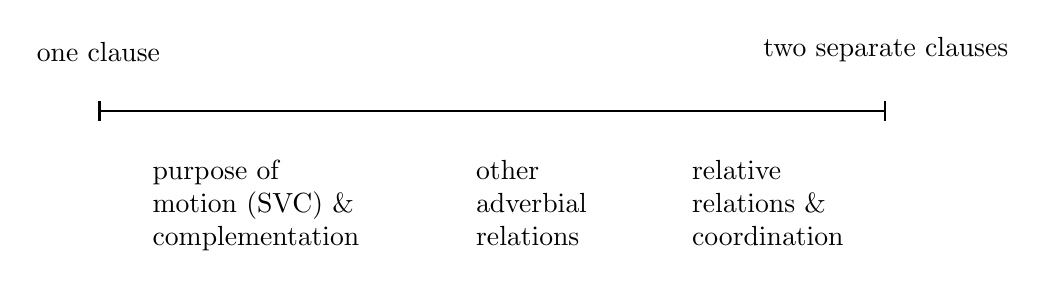
\begin{tikzpicture}
\draw [thick] [|-|]  (0,0) -- (10,0);
\node[align=left, above] at (0.0, .5){one clause};%
\node[align=right, above] at (10.0, .5){two separate clauses};%

\node[align=left, below] at (2.0,-.5)%
    {purpose of\\motion (SVC) \&\\complementation};
\node[align=left, below] at (5.5,-.5)%
    {other\\adverbial\\relations};
\node[align=left, below] at (8.5,-.5)%
    {relative\\relations \&\\coordination};
\end{tikzpicture}
}
\caption{Integration of asyndetically juxtaposed clauses}
\label{fig:IntegrationScaleAsyndeticJuxtaposition}
\end{figure}

It can be claimed that all coordinated\is{coordination} clauses and all headed\is{head} relative clauses\is{relative relation} that are asyndetically juxtaposed to another clause have a relatively high degree of independence. Nonetheless, these clauses are not totally independent or separate, because they occur in a single \isi{intonation} unit together with the clause they are combined with. On the other hand, in complementation\is{complement relation} as well as in expressions of \isi{purpose} of motion the subordinate clause lacks independent negatability,\is{negation} a sign that it is neatly integrated into the main clause (and thus perhaps not a “clause” at all). Other types of asyndetically juxtaposed adverbial clauses\is{adverbial relation} are closer to the biclausal end of the continuum than to the monoclausal one, but they are not as independent as coordinated\is{coordination} and headed relative clauses.\is{relative relation} This is bound to the fact that the RS\is{reality status} of the subordinate predicate\is{subordination} is sometimes determined in some way by the main clause predicate. Irrealis RS\is{irrealis} is necessarily found in adverbial clauses\is{adverbial relation} of the \isi{purpose} (except for purpose of motion), \isi{apprehensional} and counterfactual\is{counterfactuality} conditional types. Irrealis RS is also found in complement clauses\is{complement relation} of desiderative and manipulative predicates.\is{manipulative verb}\is{desiderative verb} The RS\is{reality status|(} of the subordinate predicate must match the one of the matrix predicate in complement clauses of knowledge and perception predicates. In purpose-of-motion expressions, RS of the \isi{purpose} predicate has to be either irrealis or identical to the motion verb.\is{reality status|)}\is{motion predicate}

(\ref{ex:Asycoor-2}) provides an example of two clauses that are coordinated by asyndetic juxtaposition. There is no sign of connection between the clauses, but the reportive marker\is{evidentiality} \textit{-ji} that occurs twice gives a hint in this case that we are probably dealing with two clauses, since it usually occurs only once per clause (but may also occur twice in one clause, so that this is indeed only a hint and no reliable evidence). 

The example comes from Juana’s account about her criminal in-law. He hid away in the forest, but came home at night to eat and sleep until he was arrested one night.

\ea\label{ex:Asycoor-2}
\begingl
\glpreamble bueno, tibÿkuputuji tinikuji\\
\gla bueno ti-bÿkupu-tu-ji ti-niku-ji\\
\glb well 3i-enter-\textsc{iam}-\textsc{rprt} 3i-eat-\textsc{rprt}\\
\glft ‘well, he came in and ate, it is said’
\endgl
\trailingcitation{[jxx-p120430l-2.147-148]}
\xe

%\ea\label{ex:Asycoor-222}
%\begingl
%\glpreamble upujaine echÿu kupeitu tiyunuji tiniku mantarina naukuji\\
%\gla upu-jai-ne echÿu kupei-tu ti-yunu-ji ti-niku mantarina nauku-ji\\
%\glb other-day-\textsc{possd} \textsc{dem}b afternoon-\textsc{iam} 3i-go-\textsc{rprt} 3i-eat tangerine there-\textsc{rprt}\\
%\glft ‘the other day in the afternoon he went, it is said, and ate a tangerine there, it is said’\\
%\endgl
%\trailingcitation{[jxx-p120430l-2.420-421]}
%\xe
%not so sure whether this is not a SVC in the end... 


For contrast with the coordinated clauses in (\ref{ex:Asycoor-2}) above, consider (\ref{ex:Asysub-1}) below, which encodes a subordinate relation, a complement clause whose predicate \textit{tinika} is also completely unmarked for linkage to the matrix predicate, but has to occur with \isi{irrealis} RS. The example was elicited from María S. and refers to her coati, which was chasing a butterfly.

 \ea\label{ex:Asysub-1}
\begingl
\glpreamble tisachu tinika churupepe\\
\gla ti-sachu ti-nika churupepe\\
\glb 3i-want 3i-eat.\textsc{irr} butterfly\\
\glft ‘it wants to eat the butterfly’
\endgl
\trailingcitation{[rxx-e150220s-1.20]}
\xe

There is little ambiguity about how to analyse the relations in the constructions that show a high degree of integration like complement clauses\is{complement relation} and serial verb constructions.\is{serial verb construction} In \isi{coordination} and in most expressions of adverbial relations,\is{adverbial relation} however, one clause is attached to another one at a higher level, the sentence. If the kind of relation between both clauses is not overtly marked by a connective, it is sometimes hard to determine whether a speaker wants to present both events as being asserted, i.e. coordinated, or one of the events as non-asserted and pre-supposed, i.e. in an \isi{adverbial relation} to the other one. It may sometimes even be the case that a clause could alternatively be analysed as a coordinated, adverbial or relative clause.

This is the case in (\ref{ex:CoC-AC-RC}). Both clauses can either be understood to represent two equally asserted facts that contribute to the realisation of the two old ladies that Juana is a speaker of Paunaka or alternatively the second clause (about understanding Paunaka) may offer the basis for the deduction expressed in the first clause or it can be analysed as a relative clause to modify a participant of the main clause. If we favour the first analysis, this is an example of \isi{coordination}, the second analysis yields an adverbial clause\is{adverbial relation} and according to the third one, we deal with relativisation here.

The sentence was produced by Juana, when she told me of an encounter with two old ladies in Candelaria who first did not recognise that she was a speaker of Paunaka.


\ea\label{ex:CoC-AC-RC}
\begingl
\glpreamble “kumade, biparienteneyenu eka pimiya chisamuyenu paunaka”\\
\gla kumade bi-pariente-ne-yenu eka apimiya chi-samu-yenu paunaka\\ 
\glb fellow 1\textsc{pl}-relative-\textsc{possd}-\textsc{ded} \textsc{dem}a girl 3-hear-\textsc{ded} Paunaka\\ 
\glft ‘“fellow, this girl must be our relative (and) she must understand Paunaka!”’ \\ or: ‘“fellow, this girl must be our relative, since apparently she understands Paunaka”’ \\or: ‘“fellow, this girl who apparently understands Paunaka must be our relative”’
\endgl
\trailingcitation{[jxx-p120515l-1.108]}
\xe

Even if we decide to analyse a clause as encoding an \isi{adverbial relation}, it is still not always clear which kind of adverbial relation is encoded as in (\ref{ex:temp-cause}), which may express a temporal (“when”) or a causal (“because”) relation. This ambiguity is also reflected in the English translation with a gerund, which leaves the specific kind of semantic connection unexpressed, just like the Paunaka predicate does. However, while the predicate in the English translation is deranked, there is no sign of dependency in the original Paunaka clause.\footnote{The translation fails to capture another peculiarity: the verb in the adverbial clause of the Paunaka example, besides not involving passivisation like the English translation, has no object marker and is thus best analysed as encoding the event in such a way that children went around and invited other children to come to school, i.e. it was not only Miguel who was invited.} The sentence stems from Miguel’s account about how he learned to read, write and calculate.

\ea\label{ex:temp-cause}
\begingl
\glpreamble komensau niyunu xhikuerayae tikupirauchunube eka punachÿ sesejinube\\
\gla komensau ni-yunu xhikuera-yae ti-kupirauchu-nube eka punachÿ sesejinube\\
\glb begin 1\textsc{sg}-go school-\textsc{loc} 3i-invite-\textsc{pl} \textsc{dem}a other children\\
\glft ‘I started to go to school being invited by other children’
\endgl
\trailingcitation{[mxx-p181027l-1.003]}
\xe

%- not clear whether coordinate or adverbial clause: jxx-p120430l-2.236, 

The question of which type of clause connection we are dealing with is of concern for translation into English, where the kind of relation between the events often needs to be expressed overtly, and it is of concern when trying to attach some labels to the examples in this grammar and sort them into different categories. It is, of course, not of concern for the speakers of Paunaka, who do not demand this kind of analysis, when speaking their language. They simply link by \isi{intonation} what belongs together.

\subsection{Syndetic juxtaposition}\label{sec:SyndeticJuxtaposition}\is{connective|(}

In syndetic juxtaposition, the predicates of both clauses are balanced,\is{finite verb} just like in asyndetic juxtaposition, but there is a linking element that specifies the kind of relation between the clauses. %These clauses have also been called adjoined clause \citep[185]{Lehmann1988}.
In Paunaka, we find syndetic juxtaposition in \isi{coordination} and in adverbial linking.\is{adverbial relation} A connective is placed between the two clauses in these cases. There is always only one connective word per connection, so we can speak of a monosyndetic pattern \citep[cf.][4]{Haspelmath2004}. We can also speak of syndetic juxtaposition in defining the construction type of most headless and a few headed\is{head} relative clauses\is{relative relation} and of a marginal type of complement clauses.\is{complement relation}\is{complementiser} However, in these cases, it is not a connective but a nominal demonstrative that serves as linker.

On the integration scale given in \figref{fig:IntegrationScaleSyndeticJuxtaposition}, syndetic complementation is possibly found far on the left-hand side, and I use the word “possibly” here, because this is really a marginal type of complementation, so that I cannot provide much information about it. Headless relative clauses share with complement clauses that they are integrated into the main clause as an argument.\is{argument} However, in contrast to complement clauses, headless relative clauses can be negated separately.\is{negation} Relative relations\is{relative relation} are thus placed right of complementation. Adverbial relations\is{adverbial relation} and \isi{coordination} are found at the right side of the scale. However, since adverbial clauses lack assertiveness, they are less independent than coordinated clauses. Since in syndetic juxtaposition both of them are overtly linked to another piece of discourse, they are both less independent than the asyndetically juxtaposed ones.

\begin{figure}
\centering
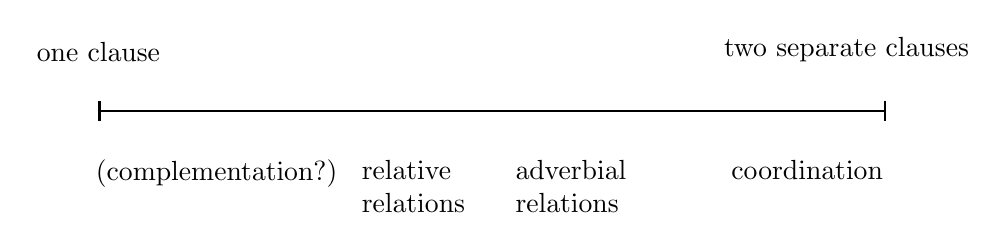
\begin{tikzpicture}
\draw [thick] [|-|]  (0,0) -- (10,0);
\node[align=left, above] at (0.0, .5){one clause};%
\node[align=right, above] at (9.5, .5){two separate clauses};%

\node[align=left, below] at (1.5,-.5)%
    {(complementation?)};
\node[align=left, below] at (4,-.5)%
    {relative\\relations};
\node[align=left, below] at (6,-.5)%
    {adverbial\\relations};
\node[align=left, below] at (9,-.5)%
    {coordination};
\end{tikzpicture}
\caption{Integration of syndetically juxtaposed clauses}
\label{fig:IntegrationScaleSyndeticJuxtaposition}
\end{figure}


As for \isi{coordination} and adverbial relations,\is{adverbial relation} there is no ambiguity as to which kind of semantic relation between the clauses is expressed, since there are several different connectives (see \sectref{sec:Conjunctions} for an overview of connective words). (\ref{ex:Syn-te-1}) involves coordination with the sequential connective \textit{te}. Like (\ref{ex:Asycoor-2}) above, it is about the last things Juana’s brother did before he suddenly died. 

\ea\label{ex:Syn-te-1}
\begingl
\glpreamble titupunubu terminalyae te tiyunu mikroyae\\
\gla ti-tupunubu terminal-yae te ti-yunu mikro-yae\\
\glb 3i-arrive bus.station-\textsc{loc} \textsc{seq} 3i-go microbus-\textsc{loc}\\
\glft ‘he arrived at the bus station and then went by microbus’
\endgl
\trailingcitation{[jxx-p120430l-2.402]}
\xe

In (\ref{ex:Syn-kue-2}) on the other hand, we have a subordinate clause, which is introduced by the connective \textit{kue} ‘if, when’. This connective marks the clause as an antecedent in a conditional sentence. The verb in the antecedent clause is not marked for subordination, but it necessarily takes \isi{irrealis} RS, since it refers to a non-factual event. The sentence was produced by Miguel, when inviting María C. to come to the workshop on Paunaka we had organised in 2011. Her husband was very ill, so she doubted that she would be able to come. Miguel was also sure that María C.’s husband could not stay at home alone.

\ea\label{ex:Syn-kue-2}
\begingl
\glpreamble kue piyuna tiyunauku echÿu\\
\gla kue pi-yuna ti-yuna-uku echÿu\\
\glb if 2\textsc{sg}-go.\textsc{irr} 3i-go.\textsc{irr}-\textsc{add} \textsc{dem}b\\
\glft ‘if you go, he has to go, too’
\endgl
\trailingcitation{[mux-c110810l.042]}
\xe

In some relative clauses,\is{relative relation} typically the headless ones, the linking element is a \isi{nominal demonstrative}, thus it is not specialised as a connective per se. The demonstrative precedes the otherwise completely unmarked clause just like it would precede a noun. This can be considered as a sign of the verb having gained some nominal characteristics. (\ref{ex:Syn-REL}) offers one example.

María C. asks Miguel here about a sheet of paper with some information about our project that Federico had given her a few days earlier.

\ea\label{ex:Syn-REL}
\begingl
\glpreamble ¿i kena echÿu chinejiku ukuinebu?\\
\gla i kena echÿu chi-nejiku ukuinebu\\
\glb and \textsc{uncert} \textsc{dem}b 3-leave some.time.ago\\
\glft ‘and what about the one he left some days ago?’
\endgl
\trailingcitation{[mux-c110810l.131]}
\xe
\is{connective|)}
\is{juxtaposition|)}
\is{syndesis/asyndesis|)}

\subsection{Dependency marking}\label{sec:ConstructionTypePA}

\is{subordination|(}
\is{dependency marking|(}
There is only one specific construction in which a \isi{finite verb} carries a dependency marker: the motion-cum-purpose construction,\is{motion-cum-purpose construction|(} in which the purpose verb is marked by the dislocative marker\is{dislocative|(} (see \sectref{sec:PA}). Although it mostly occurs within this construction, the marker is also found in other contexts that have nothing to do with dependency. It may have had primarily functions not related to subordination in older times, but this is relatively restricted today. In the motion-cum-purpose construction, the verb expressing purpose is dependent on the one expressing motion by having the same subject and the same RS. Thus, the dislocative marker can be considered a marker of this dependency. The dislocative marker occurs directly after the verb stem, but does not cause deletion of the thematic suffixes. It inflects for RS.\is{dislocative|)} 

\sloppy
Since the purpose verb in a motion-cum-purpose construction cannot be  individually negated,\is{negation} the construction belongs to the integrating monoclausal type, see \figref{fig:IntegrationScaleMCPC}.
\fussy

\begin{figure}
\centering
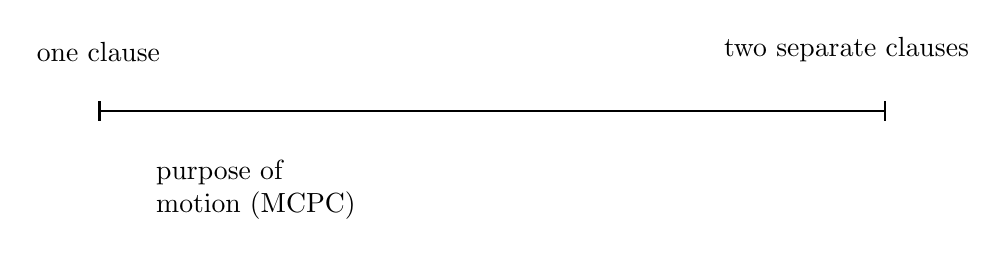
\begin{tikzpicture}
\draw [thick] [|-|]  (0,0) -- (10,0);
\node[align=left, above] at (0.0, .5){one clause};%
\node[align=right, above] at (9.5, .5){two separate clauses};%
\node[align=left, below] at (2.0,-.5)%
    {purpose of\\motion (MCPC)};
\end{tikzpicture}
\caption{Integration of verbs marked for dependency}
\label{fig:IntegrationScaleMCPC}
\end{figure}

A motion predicate,\is{motion predicate} most typically the verb \textit{-yunu} ‘go’, is combined with another verb that encodes the purpose of the motion. The purpose verb carries the \isi{dislocative} marker and is thus marked as dependent, but does not have any nominal properties in contrast to the deranked subordinate verb (see \sectref{sec:Subordination-i} below). One example of a motion-cum-purpose construction is (\ref{ex:MOC-1}). It was elicited from Miguel.

\ea\label{ex:MOC-1}
\begingl
\glpreamble niyuna ninikupa\\
\gla ni-yuna ni-niku-pa\\
\glb 1\textsc{sg}-go.\textsc{irr} 1\textsc{sg}-eat-\textsc{dloc.irr}\\
\glft ‘I will go to eat’
\endgl
\trailingcitation{[mxx-e160811sd.174]}
\xe
\is{motion-cum-purpose construction|)}

If we exchange the verb containing the dislocative marker by one with the subordinate suffix \textit{-i}, the meaning of the sentence changes. Compare to (\ref{ex:noMOC}), which was also elicited from Miguel.

\ea\label{ex:noMOC}
\begingl
\glpreamble niyuna ninikia\\
\gla ni-yuna ni-nik-i-a\\
\glb 1\textsc{sg}-go.\textsc{irr} 1\textsc{sg}-eat-\textsc{subord}-\textsc{irr}\\
\glft ‘I will go in order to eat’
\endgl
\trailingcitation{[mxx-e160811sd.176-177]}
\xe

In (\ref{ex:MOC-1}) motion is directed towards the place where the food is, and this is not necessarily the case in (\ref{ex:noMOC}), which only specifies that the speaker moves from or to a place and that the purpose for this motion is eating, but the exact relation between going and eating is not specified. Actually, though grammatically correct, speakers would normally not use a sentence like (\ref{ex:noMOC}), exactly because the relation between both predicates is too vague. The use of deranked verbs with the subordinate suffix \textit{-i} is the topic of the next section.
\is{dependency marking|)}

\subsection{Deranking}\label{sec:Subordination-i}
\is{deranked verb|(}

Active verbs can be marked as subordinate by a suffix \textit{-i}.\is{active verb}\footnote{Stative verbs do usually not take this suffix, but there are a few exceptions in the corpus, as well as a few cases in which a non-verbal predicate\is{non-verbal predication} takes the subordinate marker, e.g. the non-verbal predicate\is{motion predicate} \textit{kapunu} ‘come’ sometimes has a subordinate form \textit{kapuniu}. This shows shows how pervasive the pattern has become.} Verbs that take \textit{-i} partly lose their verbal properties. They are deranked. Deranked verbs occur in different kinds of adverbial clauses,\is{adverbial relation} in a few atypical complement clauses,\is{complement relation} in the relativisation of obliques\is{oblique} and in a specific focusing construction\is{focus} (including some questions).\is{interrogative clause} They sometimes also simply pop up for no apparent reason -- or at least no reason obvious to me. The suffix \textit{-i} can thus be considered a multi-purpose subordinator. The different constructions with a deranked verb occupy different positions on the integration scale as is illustrated in \figref{fig:IntegrationScaleDeranking}. In \isi{focus} constructions and complementation,\is{complement relation} the deranked verb constitutes an \isi{argument} and is thus completely integrated. In relative\is{relative relation} and adverbial clauses\is{adverbial relation} it acts as a modifier and as such it is also individually negatable.\is{negation} Since the clause with the deranked verb could not occur independently in this way, they occupy a middle position on the scale.

A clause with a deranked verb usually contains no other means to establish the link to another clause. Occasionally, however, we find it being combined with a \isi{preposition} in adverbial clauses\is{adverbial relation} or with a demonstrative\is{nominal demonstrative} in relative clauses.\is{relative relation} 

\begin{figure}
\centering
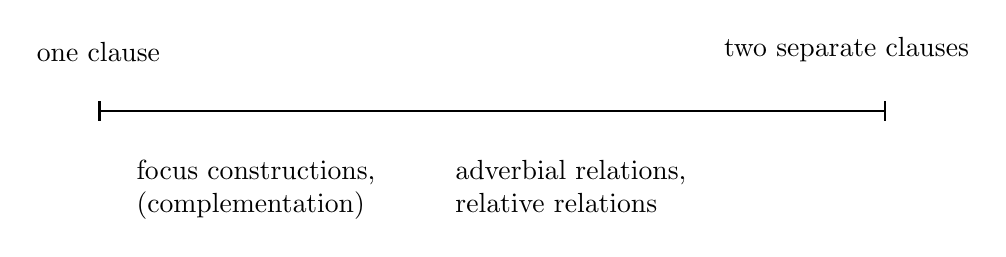
\begin{tikzpicture}
\draw [thick] [|-|]  (0,0) -- (10,0);
\node[align=left, above] at (0.0, .5){one clause};%
\node[align=right, above] at (9.5, .5){two separate clauses};%
\node[align=left, below] at (2.0,-.5)%
    {focus constructions,\\(complementation)};
\node[align=left, below] at (6.0,-.5)%
    {adverbial relations,\\ relative relations};
\end{tikzpicture}
\caption{Integration of deranked clauses}
\label{fig:IntegrationScaleDeranking}
\end{figure}

The subordinate suffix directly follows the last consonant or vowel of the stem\is{verbal stem} of an active verb, thus it directly precedes the RS\is{reality status|(} marker. This  can be seen in (\ref{ex:i-ex-1}) and (\ref{ex:i-ex-2}), which both contrast an active finite verb with its deranked form. The finite verbs are given in a) and the deranked forms in b). In (\getfullref{ex:i-ex-1.1}), we have the verb \textit{-yunu} ‘go’, which is a verb that does not take a thematic suffix. Its RS is realis by absence of any irrealis marking. In (\getfullref{ex:i-ex-1.2}), the deranked form of the verb is given, with the subordinate marker interrupting the sequence of the last stem consonant /n/ and the default vowel/realis marker \textit{-u}. It is quite unusual that a well-formed CV \isi{syllable} is broken up to insert some grammatical material in Paunaka, but exactly this happens when the subordinate marker is attached to a verb stem.\is{verbal stem} The default vowel/realis marker follows the subordinate marker and is glossed as ‘realis’ in this case.\footnote{Regarding the question why the /u/ is glossed as realis in the subordinate form \textit{-yuniu} but not in the non-subordinate verb stem \textit{-yunu}, this is discussed in \sectref{sec:VerbalRS}.} In (\getfullref{ex:i-ex-2.1}), we have a verb whose stem ends in a thematic suffix \is{thematic suffix|(} \textit{-ka} with irrealis RS in this case. The subordinate form of the verb in (\getfullref{ex:i-ex-2.2}) is built the same way as the one in (\getfullref{ex:i-ex-1.2}): the subordinate marker breaks up the sequence of the last consonant of the stem, which is thematic /k/ in this case, and the irrealis marker \textit{-a}.\is{thematic suffix|)} The deranked verbs are translated with English gerunds, which I believe most closely reflects the status of Paunaka deranked verbs.


\ea\label{ex:i-ex-1}
  \ea\label{ex:i-ex-1.1}
\begingl
\glpreamble niyunu\\
\gla ni-yunu\\
\glb 1\textsc{sg}-go\\
\glft ‘I go’
\endgl
  \ex\label{ex:i-ex-1.2}
\begingl
\glpreamble niyuniu\\
\gla ni-yun-i-u\\
\glb 1\textsc{sg}-go-\textsc{subord}-\textsc{real}\\
\glft ‘my going’
\endgl
\z
\xe


\ea\label{ex:i-ex-2}
  \ea\label{ex:i-ex-2.1}
\begingl
\glpreamble pinika\\
\gla pi-nika\\
\glb 2\textsc{sg}-eat.\textsc{irr}\\
\glft ‘you will/can/must eat’
\endgl
  \ex\label{ex:i-ex-2.2}
\begingl
\glpreamble pinikia\\
\gla pi-nik-i-a\\
\glb 2\textsc{sg}-eat-\textsc{subord}-\textsc{irr}\\
\glft ‘your (future/possible/forced) eating’
\endgl
\z
\xe


Regarding their part of speech behaviour, deranked verbs are partly verbal and partly nominal. Their verbal behaviour is bound to the way they mark RS. As we have just seen in (\ref{ex:i-ex-1}) and (\ref{ex:i-ex-2}) above, there is a suffix \textit{-u} for realis and a suffix \textit{-a} for irrealis RS. This kind of RS marking is identical to that of finite verbs, and it is exclusively found on verbs (see \sectref{sec:RealityStatus}). Paunaka also has a non-verbal irrealis marker, but it has a different form, \textit{-ina} (see \sectref{NominalRS} and \sectref{sec:NonVerbalPredication}).\is{reality status|)} 

Subordinate verbs behave like nouns\is{noun} regarding person marking.\is{person marking|(} Person markers are identical for both nouns and verbs with one exception, the third person marker \textit{ti-}, which is only found on intransitive verbs and transitive verbs with SAP objects or non-emphasised third person objects (see \sectref{sec:3Marking}). The marker \textit{chÿ-} is used to encode third person possessors on nouns,\ and on verbs it encodes 3>3 relationships. Deranked verbs always take \textit{chÿ-} for third person indexing. The marker \textit{ti-} does not occur, not even with intransitive verbs. This means that person marking on these subordinate verbs is achieved in the same way as possessor marking on nouns (see \sectref{sec:Possession}).
Consider (\ref{ex:i-ex-3}), which contrasts an intransitive finite verb taking a third person subject indexed by \textit{ti-}, with the same verb in deranked form that takes the marker \textit{chi-} (an allomorph of \textit{chÿ-}).

\ea\label{ex:i-ex-3}
  \ea\label{ex:i-ex-3.1}
\begingl
\glpreamble tiyunu\\
\gla ti-yunu\\
\glb 3i-go\\
\glft ‘he/she/it goes’
\endgl
  \ex\label{ex:i-ex-3.2}
\begingl
\glpreamble chiyuniu\\
\gla chi-yun-i-u\\
\glb 3-go-\textsc{subord}-\textsc{real}\\
\glft ‘his/her/its going’
\endgl
\z
\xe


According to \citet[69]{Cristofaro2003}, “[s]ome languages express person agreement distinctions in the dependent clause by means of possessive affixes”, and by doing so, they “reflect a conceptualization of the dependent SoA as a thing rather than a process” \citep[285]{Cristofaro2003}, i.e. the subordinate predicate is integrated into the main clause as a “unitary whole” rather than a process that involves a sequence of different states that have to be cognitively processed in succession \citep[262]{Cristofaro2003}.
However, the fact that Paunaka marks subjects\is{subject} of deranked verbs like possessors should not be overemphasised, since the effect of using possessor markers instead of subject markers is considerably small. It is only visible with a small number of verbs after all: intransitives with a third person subject and transitives with a third person subject and an SAP object. 
\is{person marking|)}

Apart from the person marker, there is usually nothing else on the deranked verb that could indicate its nominal status. There are cases in which speakers translate deranked verbs to Spanish with a \isi{finite verb} and other cases in which they find a noun more appropriate. It is typically action nominalisations\is{nominalisation} %of the event type, sometimes also of the result type
 \citep[cf.][335]{ComrieThompson2007} they use in the latter cases. While translation to another language certainly does not prove the status of the word in the source language, it can be taken as proof that Paunaka uses deranked verbs in situations that are cross-linguistically apt to be encoded by finite verbs as well as situations that can cross-linguistically be associated with \isi{nominalisation}.

There are even a few cases in which a deranked verb takes a locative marker (see \sectref{sec:Locative}). This is regularly done with the word \textit{-ubiu} ‘house’, as in (\ref{ex:sub-loc}). The word must have arisen as a subordinate verb, but is now best considered a noun with the meaning ‘house’ (due to a former lexicalisation process). In addition to frequently taking the locative marker, it also takes the non-verbal irrealis marker. (\ref{ex:sub-loc}) and (\ref{ex:sub-irrnv}) provide two examples of the word \textit{-ubiu} ‘house’ with nominal morphology, the locative marker \textit{-yae} and the non-verbal irrealis marker \textit{-ina} respectively. (\ref{ex:sub-loc}) provides an analysis in which the noun is split into its separate morphemes to show its origin as a deranked verb, and in (\ref{ex:sub-irrnv}) the full form \textit{-ubiu} is glossed as a noun ‘house’, which is the way I usually analyse this word in the grammar.\footnote{In addition to the inalienably possessed noun \textit{-ubiu} ‘house’, there is also a free form \textit{ubiae} ‘house’, which most probably goes back to a deranked verb as well, but with irrealis marking: \textit{ub-i-a} be-\textsc{subord}-\textsc{irr}. The /e/ attached to the end of this word could go back to a nominalising suffix\is{nominalisation} that is not productive anymore. Compare Mojeño\is{Mojeño languages} \textit{-re} (\citealt[630]{OlzaZubiri2004}; \citealt[85]{Rose2014a}) and remember that Paunaka lost /ɾ/ (see \sectref{phonology_r}). A few cases of a nominalising \textit{-e} in Paunaka are described in \sectref{sec:MorphologyNominalisation}.}


\ea\label{ex:sub-loc}
\begingl
\glpreamble pitupunubutu nubiuyae\\
\gla pi-tupunubu-tu nÿ-ub-i-u-yae\\
\glb 2\textsc{sg}-arrive-\textsc{iam} 1\textsc{sg}-be-\textsc{subord}-\textsc{real}-\textsc{loc}\\
\glft ‘you have arrived at my house’
\endgl
\trailingcitation{[rxx-e181017l]}
\xe

\ea\label{ex:sub-irrnv}
\begingl
\glpreamble kuina nubiuna\\
\gla kuina nÿ-ubiu-ina\\
\glb \textsc{neg} 1\textsc{sg}-house-\textsc{irr}\\
\glft ‘I don’t have a house (in Santa Cruz)’
\endgl
\trailingcitation{[rxx-e120511l.233]}
\xe

Locative marking\is{locative marker} is rarely found with other deranked verbs, but consider (\ref{ex:sub-nom}), which was also translated to Spanish by María S. with a noun, \textit{carta} ‘letter’. There are no other cases to my knowledge in which a deranked verb takes the \isi{non-verbal irrealis marker}.

\ea\label{ex:sub-nom}
\begingl 
\glpreamble chisuikiuye\\
\gla chi-suik-i-u-yae\\ 
\glb 3-write-\textsc{subord}-\textsc{real}-\textsc{loc}\\ 
\glft ‘in her letter’
\trailingcitation{[rxx-e121128s-1.026]}
\xe

%chibitakiane with possessed suffix -> conversion to noun completed, but only this one in corpus? or conversion to noun completed, when they are modified by a demonstrative?

Deranked verbs have been found in combination with prepositions\is{preposition} in some subclasses of adverbial clauses,\is{adverbial relation} another indication for their partly nominal status. Consider (\ref{ex:paper-go}), which has a purpose clause with a deranked verb preceded by the preposition \textit{tÿpi} ‘\textsc{obl}’.\is{general oblique}

The sentence was produced by Miguel to explain to María C. the content of a leaflet with information about the workshop on Paunaka held in 2011.

\ea\label{ex:paper-go}
\begingl
\glpreamble eka ajumerku tÿpi piyunia nauku unekuyae reunion\\
\gla eka ajumerku tÿpi pi-yun-i-a nauku uneku-yae reunion\\
\glb \textsc{dem}a paper \textsc{obl} 2\textsc{sg}-go-\textsc{subord}-\textsc{irr} there town-\textsc{loc} meeting\\
\glft ‘this paper is for you to go to the meeting in town’
\endgl
\trailingcitation{[mux-c110810l.012]}
\xe


TAME marking\is{tense}\is{aspect}\is{modality}\is{evidentiality} on deranked verbs is very restricted. A few cases of \isi{iamitive} and \isi{uncertainty} marking occur, but they are so rare that they should be considered exceptional. Thus, we can state that in general TAME marking is lacking on deranked verbs, which is cross-linguistically quite frequent in subordination \citep[cf.][66]{Cristofaro2003}.  
%Subordinate verbs can take the following markeres: -nube, -mÿnÿ, -chÿ, -tu (very few examples), -kena, -jane, -pi (2sg) (?).

Sometimes the third person marker\is{person marking|(} \textit{-chÿ} occurs with deranked verbs, which is remarkable because it is unusual that non-subordinate verbs take this marker (see \sectref{sec:3Marking}). Nouns do not take it at all. Its presence on deranked verb may be motivated by the neutralisation of the distinction usually encoded by the two third person markers \textit{ti-} and \textit{chÿ-}, with the latter one overtly encoding that there is a third person \isi{object}. Object marking by \textit{-chÿ} often occurs when the subordinate verb has a different \isi{subject} than the main clause predicate and additionally its object is not identical with an \isi{argument} of the main clause. This is not restricted to verbs with third person subjects though, as can be seen in (\ref{ex:sub-3suf}), which comes from elicitation with Miguel. For more examples see \sectref{sec:3_suffixes}. 
It is not totally clear to me why deranked \isi{transitive} verbs are in general more prone to take third person markers that follow the stem than finite ones, even in constellations like (\ref{ex:sub-3suf}), in which a corresponding finite verb would not index a third person object. It does not seem to depend on presence or absence of a conominal object.

\ea\label{ex:sub-3suf}
\begingl
\glpreamble nibÿchekubi pupuniachÿ nijinepÿi\\
\gla ni-bÿcheku-bi pi-upun-i-a-chÿ ni-jinepÿi\\
\glb 1\textsc{sg}-order-2\textsc{sg} 2\textsc{sg}-bring-\textsc{subord}-\textsc{irr}-3 1\textsc{sg}-daughter\\
\glft ‘I sent you to pick up my daughter’
\endgl
\trailingcitation{[mxx-e160811sd.301]}
\xe
\is{person marking|)}

I have not found a descriptive term that would well fit Paunaka’s deranked verbs. The closest related, but not totally matching concept is that of a converb. According to the definition given by \citet[3]{Haspelmath1995}, a converb is “a nonfinite verb form whose main function is to mark adverbial subordination”. I have shown above that deranked verbs are arguably less finite than non-subordinate verbs, considering that they index subjects like possessors and in general do not mark TAME distinctions, but I would not define them as completely nonfinite, since they inflect for RS in just the same way that non-subordinate verbs do, with RS beside person being the only category that is obligatorily expressed on verbs. In addition, deranked verbs are indeed used in adverbial clauses,\is{adverbial relation} but also found in relativisation,\is{relative relation} marginally in complementation\is{complement relation} and in \isi{focus} constructions. I am not sure whether adverbial subordination\is{adverbial relation} can be considered their “main function”. Comparison with other Amazonian languages\is{Amazonian language} does not help solve the terminological issue: In Hup, a Nadahup language spoken in the Vaupés region on both sides of the Brazilian and Columbian border, \citet[]{Epps2009} found a multi-purpose dependency marker that occurs on relative as well as adverbial clauses; she uses the term “converb” only if a verb that is marked for dependency in this way occurs in an adverbial clause. When it occurs in relative clauses, she uses the term “relative” instead. Since I am more interested in finding a term that describes the verb form rather than its function in different clauses, I refrain from the use of “converb” in this grammar, but rather speak of “deranked verb”, subordinate verb marked by \textit{-i} or the like whenever I refer to a verb that is marked as subordinate in this way.\footnote{It should be noted at this place that Rose (2021, p.c.) analyses a cognate form of the subordinate marker \textit{-i} as an \isi{applicative} suffix in Trinitario.\is{Mojeño Trinitario} However, it seems that the Trinitario verbs containing this suffix do not occur in all of the contexts found with the Paunaka marker. In Trinitario, verbs with the suffix mainly show up in main clauses with an unmarked and preposed oblique (i.e. the applied object). Although this is also found in Paunaka (see \sectref{sec:AdverbialModification}), an analysis as \isi{applicative} fails to explain other contexts. As for \isi{Baure}, \citet{Danielsen2007,Danielsen2011a} relates the cognate form to locative subordination. Some of the examples she gives could also qualify as proof of the \isi{applicative} hypothesis, but not all of them. A thorough comparison between all three languages, possibly also taking into account \isi{Terena}, is certainly desirable.}

Considering the many different environments in which these deranked verbs occur, what is the common function of the subordinator \textit{-i} in Paunaka? All of the cases in which deranked verbs are found have in common that a dependency of the subordinate verb to another clause is \textit{overtly} expressed. Sometimes it just seems necessary to be explicit about a dependent relation. In adverbial clauses,\is{adverbial relation} deranked verbs mark that the clause has to be interpreted in relation to another clause, that the connection is not coincidental, but involves reason, \isi{purpose} or non-incidental temporal overlap.\is{temporal overlap/condition} As regards complement clauses,\is{complement relation} deranked verbs are used whenever an unusual relation is involved, e.g. because the matrix verb does not normally take clausal complements. In relative clauses,\is{relative relation} deranked verbs occur in the relativisation of obliques,\is{oblique} which are found on the right side of the relativisation hierarchy, i.e. are cross-linguistically found more rarely in relative clauses and are thus possibly more difficult to access. Last, deranked verbs can also be used to indicate that the preposed constituent has a special discourse status. In all of these cases, the actual process encoded by the verb is downplayed in order to emphasise that another relation, be that another process or a stative relation, is more prominent, more important for the development of discourse (see also \sectref{sec:AdverbialModification}, where this issue is discussed in more detail.)

The use of deranked verbs is the most overt means in Paunaka to mark subordinate status of a predicate. In using a deranked verb a Paunaka clause comes as close as possible to what constitutes a typical embedded clause:\is{embedding} a subordinate clause including a less finite verb filling the role of an \isi{argument} or modifier in its main clause \citep[cf.][184]{Lehmann1988}. In \isi{focus} constructions and complementation,\is{complement relation} the deranked verb acts like an \isi{argument}, in relative clauses\is{relative relation} and adverbial clauses\is{adverbial relation} as a modifier.\is{modification} Deranked verbs are in general independently negatable,\is{negation} though this may be rare in actual discourse.
\is{deranked verb|)}

A few cases of full nominalisation in subordination have also been found in the corpus. This is the topic of the next section.

\subsection{Nominalisation}\label{sec:SyntaxNominalisation}
\is{grammatical nominalisation|(}

It has been noted over and over again that nominalisation is a widespread strategy in subordination marking throughout South American languages (e.g. \citealt[19]{DerbyshirePullum1986}; \citealt[10--13]{Gijnetal2011}; \citealt[332--334]{Aikhenvald2012}). Nominalised verbs are also found in subordinate clauses of closely related \isi{Baure} \citep[]{Danielsen2011a},\footnote{Actually, the \isi{Baure} participles with the suffix \textit{-cho} come relatively close in function to Paunaka’s deranked verbs, but the latter are found in more contexts. Different kinds of relative clauses build on different kinds of nominalisers in \isi{Baure} \citep[cf.][]{Danielsen2011a}.} so why does Paunaka use a different strategy?

The nominaliser \textit{-kene} is only rarely used in current Paunaka in general, including in lexical nominalisations, see \sectref{sec:MorphologyNominalisation}. New nouns do not seem to be derived with it at all. Instead of this, finite verbs can take a demonstrative and be used like a noun, this is analysed as a case of (headless) relativisation (see \sectref{sec:HeadlessRC}).

In the recordings by Riester from the 1950s, however, we find more nominalised verbs than in the recordings made by the PDP and colleagues between 2008 and 2018. A few of them can be analysed as being used for subordination purposes. 

In (\ref{ex:NMLZ-a1}), the nominalised verb seems to express the \isi{purpose} of the main verb, i.e. an \isi{adverbial relation}. Juan Ch. is speaking about his \textit{patrón} who is supposed to support his workers.\footnote{The exact context of this utterance is not clear, unfortunately. Shortly before, Juan Ch. had been complaining about the \textit{patrón}, what follows is unintelligible, and then he speaks about all the meat the workers get, which is the passage the example is taken from. Shortly after, he goes on and speaks about how bad nutrition is, but this, apparently, was in times before. While Juana and Miguel did not agree on the exact wording here, time setting in former times was recognised by both.}

\ea\label{ex:NMLZ-a1}
\begingl
\glpreamble tikupaiku ÿba binikeneina\\
\gla ti-kupaiku ÿba bi-ni-kene-ina\\
\glb 3i-slaughter pig 1\textsc{pl}-eat-\textsc{nmlz}-\textsc{irr}\\
\glft ‘he slaughters a pig for us to eat’
\endgl
\trailingcitation{[nxx-p630101g-2.45]}
\xe


In (\ref{ex:NMLZ-q1}), we have a nominalised verb following \textit{juchubu} ‘where’, which is used as an \isi{indefinite pronoun} here. The nominalised verb thus functions as a relative clause that specifies the indefinite pronoun.\footnote{The analysis as a nominalised verb depends on the presence of the non-verbal irrealis marker \textit{-ina} here. Consider (\ref{ex:RCchija2}) in \sectref{sec:IndefinitePronouns}, which is from the same context and structurally similar. The form \textit{-kine} is analysed as emphatic marker there, since the verb carries a verbal irrealis prefix (see also \sectref{sec:EmphMarker}).} In current Paunaka, it is rather a balanced verb\is{finite verb} that is used in such constructions (see \sectref{sec:IndefinitePronouns}). In this sentence, Juan Ch. states that even if he wanted to leave Retiro, the place where he was living and working for his \textit{patrón}, there was no place that he could go to.

\ea\label{ex:NMLZ-q1}
\begingl
\glpreamble kuina juchubu biyunukeneina\\
\gla kuina juchubu bi-yunu-kene-ina\\
\glb \textsc{neg} where 1\textsc{pl}-go-\textsc{nmlz}-\textsc{irr.nv}\\
\glft ‘there is nowhere we could go’
\endgl
\trailingcitation{[nxx-p630101g-1.177]}
\xe

It is, of course, impossible to draw conclusions from two examples, but given the higher frequency of nominalised verbs in Juan Ch.’s speech in general, it seems possible that nominalised verbs were once used a lot more than today and possibly with a wider array of functions including subordination. 
\is{grammatical nominalisation|)}
\is{subordination|)}
\is{verb|)}

To sum up, this section has shown different possibilities of combining clauses and construing complex clauses: asyndetic juxtaposition, syndetic juxtaposition, dependency marking, and deranking. Full nominalisation does not play a major role and is thus neglected in everything that follows. The following sections describe the different semantic-functional subtypes in clause combining and complex clause formation. 


%!TEX root = 3-P_Masterdokument.tex
%!TEX encoding = UTF-8 Unicode

\section{Coordinated clauses}\label{sec:Coordination}\is{coordination|(}
\largerpage[-2]
Coordination has been defined by \citet[34]{Haspelmath2004} as follows: “The term \textit{coordination} refers to syntactic constructions in which two or more units of the same type are combined into a larger unit and still have the same semantic relations with other surrounding elements”. As for the term “syntactic construction”, I consider only those clauses as coordinated that occur within the same intonation unit \citep[332]{Mithun1988}. Since I have not undertaken a full-fledged analysis of intonation patterns, one \isi{intonation} unit is defined mainly on the basis of pauses, i.e. in one intonation unit there is no pause between the two clauses. In addition, if intonation is not falling at the end of a clause, this is considered a further sign of connectedness to a second one. In contrast to subordination, all clauses in coordination are asserted.

Coordination of clauses is signalled by either asyndetic \isi{juxtaposition} or syndetic \isi{juxtaposition} with a \isi{connective} (see \sectref{sec:AsyndeticJuxtaposition} and \sectref{sec:SyndeticJuxtaposition} for a general discussion of the construction types). The structure of asyndetically and syndetically coordinated clauses is given in \figref{fig:CoordinationStructure}.\is{syndesis/asyndesis}

\begin{figure}


[[MC] [MC]]

[[MC] co [MC]]
\caption{Sentence structure of juxtaposed coordinated clauses}
\label{fig:CoordinationStructure}

\end{figure}

As for asyndetic \isi{juxtaposition}, this is found mostly for \isi{conjunctive} and \isi{sequential} coordination. In syndetic \isi{juxtaposition}, connectives\is{connective|(} specify the kind of connection between the two clauses.\is{syndesis/asyndesis} The connectives used in coordination are given in \tabref{table:ConnectivesCoordination}. Apart from \textit{te} ‘then’ and \textit{nechikue} ‘therefore’, all of them have been borrowed\is{borrowing} from Spanish, which is not surprising considering the high degree of borrowability of connectives in general \citep[cf.][194]{Matras2009}.  All coordinating connectives not only combine clauses uttered within one intonation unit,\is{intonation|(} but also occur at the beginning of clauses that form their own intonation unit. The latter is analysed as discourse connection, not clause combining, i.e. the connective is used to link a piece of information to an entire episode, a feature which may just be typical for spoken mediality \citep[cf.][]{Chafe1988}.\is{connective|)} I will confine the discussion to coordination of clauses here, i.e. those uttered within one intonation unit, although the distinction between clause connection and discourse connection is certainly a gradual one.\is{intonation|)}\footnote{For a preliminary analysis of discourse connection see \citet[138--142]{DanielsenTerhart2015}.} Verbs in coordinated clauses are never deranked or marked for dependency -- at least not for the sake of signalling linking. RS\is{reality status|(} of both clauses is usually independent from each other with one exception: if the first clause encodes \isi{future reference} by having irrealis RS, a coordinated clause that expresses consequence\is{consecutive} or temporal succession\is{sequential} cannot have realis RS. This does not exclude the combination of irrealis and realis clauses for other reasons.\is{reality status|)}

\begin{table}
\caption{Connectives in coordinated clauses}

\begin{tabular}{lll}
\lsptoprule
Connective & Translation & Clause type \cr
\midrule
\textit{entonses} & thus & consecutive coordination\cr
\textit{i} & and & conjunction\cr
\textit{nechikue} & therefore & consecutive coordination\cr
\textit{o} & or & disjunction\cr
\textit{pero} & but & adversative coordination\cr
\textit{te} & ‘\textsc{seq}’ (‘then’) & sequential coordination\cr
\lspbottomrule
\end{tabular}

\label{table:ConnectivesCoordination}
\end{table}

\largerpage[-2]
The remainder of this section is organised as follows. \sectref{sec:AsyndeticCoordination} deals with asyndetic coordination, and the other sections deal with coordinated clauses that are linked by a connective: \sectref{sec:SequentialCoordination} is about sequential coordination including the connective \textit{te} ‘then’, \sectref{sec:ConjunctiveCoordination} deals with conjunctive coordination with the connective \textit{i} ‘and’, in \sectref{sec:DisjunctiveCoordination} disjunctive coordination with the connective \textit{o} ‘or’ is described, \sectref{sec:AdversativeCoordination} is about adversative coordination with \textit{pero} ‘but’ and finally, \sectref{sec:ConsecutiveCoordination} deals with consecutive coordination, a minor type of clause combining, with the connectives \textit{nechikue} ‘therefore’ and \textit{entonses} ‘thus’.

\subsection{Asyndetic coordination}\label{sec:AsyndeticCoordination}
\is{juxtaposition|(}

%tiberiukupunu tiyunupunu = she turned around and went home, mox-n110920l.077
%parikiyu chamayuchÿ aa año año trabakuyunubechi kuina kuina chisiupuchanube, mxx-p110825l.047

%nejujumi kuina nimuka yuti, jxx-p120515l-1.188
%tibÿkupunube kuina takÿraina = entraron y no había gallina, jmx-n120429ls-x5.326
%kuina nenaina echÿu gansojane tirÿrÿ chisikuji, jrx-c151001lsf-11.040


%kuina nÿnapÿka nÿbanenepuna = no vengo primero, vengo atrás, rxx-e141230s.167
%kuina tipajÿka naka kapunuina tukiu pasauna = no se queda aquí, va a venir de paseo (Federico, who lives in Conce), jxx-p110923l-1.122
%"aa nÿchÿnumi aa pensaikune kuina nitupa echÿu bakajane tijekupupuikutu", tikechu, mxx-n151017l-1.32

%nikutiutu nisuiu, kuina auantauneinabu nisua, cux-c120414ls-2.035-036

%niyunu nÿsupu kuina abansaunÿina tupirujiyu tipÿneji, rxx-e181022le
%nechikue kuina tikechunubebu kuina bichujijikabu kuina beteumichabu chimutu = y ya no decimos nada ya no le hablamos ya no le avisamos porque ya lo ha visto, nxx-p630101g-1.080
%bepaka tanÿma kuina taechunanube bijinepuinube ... bichechajinube? = nosotros nos murimos y ya no aprenden nuestro shijos y hijas, jxx-x110916.08
%kui nepakatu kuina taichunanube nimijÿnajinube niyÿsebÿkeunube kuina tisacha, jxx-x110916.48


Clauses can be coordinated by simply juxtaposing them. They occur within one \isi{intonation} unit, but there is no morphosyntactic signal of connection. These clauses are asyndetically coordinated,\footnote{Asyndetic juxtaposition is also found in coordination of NPs,\is{noun phrase} consider (\ref{ex:motherfather}):

\ea\label{ex:motherfather}
\begingl
\glpreamble nÿenu nÿa tebuku amuke\\
\gla nÿ-enu nÿ-a ti-ebuku amuke\\
\glb 1\textsc{sg}-mother 1\textsc{sg}-father 3i-sow corn\\
\glft ‘my mother and my father sowed corn’
\endgl
\trailingcitation{[rxx-p181101l-2.200]}
\xe}
as (\ref{ex:new23-asycor}), in which Juana tells me why her brother died.

\ea\label{ex:new23-asycor}
\begingl
\glpreamble ... kuina puero tinika kuina puero tea\\
\gla kuina puero ti-nika kuina puero ti-ea\\
\glb \textsc{neg} can 3i-eat.\textsc{irr} \textsc{neg} can 3i-drink.\textsc{irr}\\
\glft ‘he couldn’t eat and drink’
\endgl
\trailingcitation{[jxx-p120430l-2.370]}
\xe

According to \citet[335]{Mithun1988}, in asyndetic coordination clauses “conjoined with no intonation break typically describe subparts of what is conceived of as a single event. One clause typically sets the stage for the other by positioning a major participant. [...] By contrast, clauses separated by comma intonation typically represent conceptually distinct aspects of an action, event, or scene. The conjoined clauses most often describe sequential actions”. Alternatively, the latter can also “describe simultaneous aspects of a scene or state” \citep[336]{Mithun1988}. As for the notion of “single event”, this is hard to prove, because whether something is perceived as a single event or as multiple connected events is connected to cognitive processes, which I do not have access to.\footnote{\citet[]{Defina2016} describes an interesting approach, considering gestures co-occurring with serial verbs as indication of whether a sequence of verbs is considered as one or several events. This approach requires excellent video recordings, something that could be worth collecting in the future as long as there are still speakers available.} Or, as \citet[306]{Haspelmath2016} states, “there is no objective way of identifying a single event and distinguishing it from a set of several events”. For the time being, I do not make any distinctions between single and multiple events.

What we do find in coordination of clauses in Paunaka is that one clause sets the stage for another one by mentioning a participant. Both of these clauses typically have the same RS.\is{reality status}\footnote{I do not follow \citet[]{Mithun1988} in making a distinction between coordination of predicates and clauses, since a single predicate can be a full clause in Paunaka, see \sectref{sec:WordOrder}.} They usually share at least one participant and often but not always describe \isi{sequential} actions.

Consider (\ref{ex:lift-take}), where subject and object of both clauses are identical. A participant, \textit{echÿu jente} ‘the man’, is introduced as an object by a conominal NP in the first clause. The man is already well-established in the story, but not accessible as a possible object of the verb. This very same participant also acts as an object of the second clause, this time without being conominated. The subject of both clauses is topical and thus not conominated. The sentence stems from the tale told by María S. about the two men who meet the devil. The devil demands food and one man gives it to him. When the food is finished, the devil is still hungry, so he grabs the man and takes him with him in order to eat him.

\ea\label{ex:lift-take}
\begingl
\glpreamble chakachutuji echÿu jente chumu\\
\gla chÿ-akachu-tu-ji echÿu jente chÿ-umu\\
\glb 3-lift-\textsc{iam}-\textsc{rprt} \textsc{dem}b man 3-take\\
\glft ‘he picked up the man, it is said, and took him (with him)’
\endgl
\trailingcitation{[rxx-n120511l-2.57]}
\xe

In (\ref{ex:jump-fall}), the conominated object participant of the first verb, \textit{aitubuchepÿimÿnÿ} ‘little boy’, is a raised possessor\is{possessor raising} belonging to the incorporated\is{incorporation} body part \textit{-bÿke} ‘face’. It acts as the subject of the second, intransitive verb without being conominated again. The example stems from Miguel’s description of the \isi{frog story}, more precisely the picture in which the owl flies out of its hole in the tree and boy falls from the tree.

\ea\label{ex:jump-fall}
\begingl
\glpreamble i chijipubÿkejukukena eka aitubuchepÿimÿnÿ tibÿtupaikubu tukiu anÿke\\
\gla i chi-jipu-bÿke-ju-ku-kena eka aitubuchepÿi-mÿnÿ ti-bÿtupaikubu tukiu anÿke\\
\glb and 3-jump-face-?-\textsc{th}1-\textsc{uncert} \textsc{dem}a boy-\textsc{dim} 3i-fall from up\\
\glft ‘and it seems that it jumps into the face of the little boy and he falls down from above’
\endgl
\trailingcitation{[mox-a110920l-2.102]}
\xe

In (\ref{ex:lift-fish}), the subject of both verbs is identical. However, the participant \textit{chÿkuaji} ‘her fishing net’, which is introduced in the first clause, is not in a grammatical relation to the predicates of the second clause, two verbs in a motion-cum-purpose construction (see \sectref{sec:MotionCumPurpose}). However, the fishing net sets the ground semantically for the second clause, which is about fishing. Even more so, the verb \mbox{\textit{-epuiku}} ‘fish’ is only used for fishing with a net; when the Paunaka speak about fishing with a hook, they use a different verb. This example was produced by María C. to illustrate that her mother did not care for her, when she had a difficult birth and was weak by loss of blood.


\ea\label{ex:lift-fish}
\begingl
\glpreamble chakapaiku chÿkuaji tiyunu tepuikupu\\
\gla chÿ-akapaiku chÿ-kuaji ti-yunu ti-epuiku-pu\\
\glb 3-lift 3-net 3i-go 3i-fish-\textsc{dloc}\\
\glft ‘she picked up her net and went fishing’
\endgl
\trailingcitation{[ump-p110815sf.433]}
\xe

We also find asyndetic juxtaposition in coordination of clauses with SAP participants. This is the case in (\ref{ex:go-come}), in which both clauses have first person plural subjects. With this sentence, Miguel states that they went away from \isi{Altavista} and came to Santa Rita.

\ea\label{ex:go-come}
\begingl
\glpreamble biyunu bibÿsÿupunutu naka\\
\gla bi-yunu bi-bÿsÿupunu-tu naka\\
\glb 1\textsc{pl}-go 1\textsc{pl}-come-\textsc{iam} here\\
\glft ‘we went and then came here’
\endgl
\trailingcitation{[mqx-p110826l.380]}
\xe


Except for (\ref{ex:jump-fall}), in all examples presented up to here, the subjects of both coordinated clauses were identical. Another example of coordinated clauses with non-identical subjects is (\ref{ex:inscribe-stay}). The first person participant is introduced as the object of the first clause by being indexed on the verb with the marker \textit{-nÿ}, and then it acts as the subject of the intransitive verb in the second clause, being indexed by the marker \textit{ni-}. The sentence comes from Miguel’s account about how he acquired literacy and learned to calculate and it refers to the school.

\ea\label{ex:inscribe-stay}
\begingl
\glpreamble bueno, tisuichunÿtu echÿu profesor nipajÿkutu\\
\gla bueno ti-suichu-nÿ-tu echÿu profesor ni-pajÿku-tu\\
\glb well 3i-inscribe-1\textsc{sg}-\textsc{iam} \textsc{dem}b teacher 1\textsc{sg}-stay-\textsc{iam}\\
\glft ‘well, the teacher inscribed me and I stayed’
\endgl
\trailingcitation{[mxx-p181027l-1.019]}
\xe

The examples I have given up to this point resemble the ones cited by \citet{Mithun1988} to exemplify her category of “coordination by intonation”, i.e. asyndetic coordination.\is{intonation} However, many of them equally resemble the ones given by \citet{Aikhenvald2006,Aikhenvald2018} and \citet{Haspelmath2016} as  proof for another syntactic construction, namely the serial verb construction.\is{serial verb construction|(} This is because in all examples so far, at least one participant is shared, the verbs are often adjacent and they share the same RS.\is{reality status} I prefer the term asyndetic coordination over serial verb construction nonetheless. 

First of all, in an attempt to distinguish serial verbs from coordinated verbs, \citet[3,24,125-127]{Aikhenvald2018} proposes that the meaning changes if one inserts a connective\is{connective|(} between the verbs, i.e. serial verbs cannot be rephrased with a sequence of syndetically coordinated clauses. I have not tried this with the examples in this section, but my hypothesis is that nothing would change substantially if connectives were used. There are similar examples that do contain connectives (especially \isi{sequential} \textit{te} and \isi{conjunctive} \textit{i}, see \sectref{sec:SequentialCoordination} and \sectref{sec:ConjunctiveCoordination}).\is{serial verb construction|)} One factor in the choice between asyndetic and syndetic\is{syndesis/asyndesis} coordination I could identify is that the former is preferred if the time lapse between the events described by the two verbs is minimal as in (\ref{ex:lift-take}) above or also in (\ref{ex:snake-pull}) below. The situation described here is dangerous and thus requires quick and immediate action. The sentence comes from Juana, who was telling me how her sister María S. once met a snake (or water spirit), when she was bathing in the reservoir. Her husband saved her from being attacked.

\ea\label{ex:snake-pull}
\begingl
\glpreamble kapunu chima chijatÿku\\
\gla kapunu chÿ-ima chi-jatÿku\\
\glb come 3-husband 3-pull\\
\glft ‘her husband came and pulled her (out of the water)’
\endgl
\trailingcitation{[jxx-p120515l-2.168]}
\xe

In contrast, consider (\ref{ex:father-come}), which has the same predicates as (\ref{ex:lift-take}), but takes a \isi{sequential} connective \textit{te} (see \sectref{sec:SequentialCoordination}). It stems from Juana’s account about her grandparents, who lost the cows they had bought, because a \textit{karay} took them away. Apparently, Juana’s father found two of them in the pampa and brought them to \isi{Altavista}, where he lived at that time. The action of taking cows probably requires some preparation, and we can thus assume a bigger time lapse to the first action of coming.

\ea\label{ex:father-come}
\begingl
\glpreamble kapunu nÿabane te chumu nauku Turuxhiyaebane\\
\gla kapunu nÿ-a-bane te chÿ-umu nauku Turuxhi-yae-bane\\
\glb come 1\textsc{sg}-father-\textsc{rem} \textsc{seq} 3-take there Altavista-\textsc{loc}-\textsc{rem}\\
\glft ‘my late father came and took them to old Altavista’
\endgl
\trailingcitation{[jxx-e150925l-1.238]}
\xe

%kapunu punachÿ kayaraunu te chupunu chipeu baka, jxx-e150925l-1.250

This does, however, neither imply that a connective is impossible in expressing \isi{sequential} events with minimal time lapse nor that it is required when time lapse between two events is bigger.\is{connective|)}

The second reason why I prefer to analyse the examples in this section as cases of asyndetic coordination rather than as serial verbs\is{serial verb construction|(} is connected to grammatical integration: a crucial feature of serial verb constructions according to the definitions by \citet[296]{Haspelmath2016} and by \citet[1]{Aikhenvald2006} is that they are monoclausal.\is{negation|(} Consequently, they can only be negated in one way with negation having scope over both predicates \citep[299]{Haspelmath2016}. There are some construction types in Paunaka that fulfil this criterion, i.e. a serial verb construction with the motion verb \textit{-yunu} ‘go’ in which the second verb specifies the purpose of motion (see \sectref{sec:SerialVerbs}) and cases of complementation (see \sectref{sec:ComplementClauses}), but it is not clear whether the examples presented here could be defined as monoclausal by the criterion of (possible) negation having scope over both predicates. In general, clauses with negated predicates are seldom coordinated to other clauses in Paunaka, and if so, they usually have a \isi{connective} word.\is{serial verb construction|)}\footnote{\label{fn:negation-coordination}What we do find regularly is that first a negative clause is uttered and then the negator \textit{kuina} is repeated at the beginning of the next sentence. It is pronounced with a slightly falling \isi{intonation} and followed by a short pause. Juxtaposed to this negator, we find a positive clause, see (\ref{ex:neg-fn-1}). We can thus speak of one clause containing only the negator, which is coordinated to a positive clause. Word order would be identical if this was a single negative clause, but it would have a different intonation contour and no pause would occur between the negator and the following predicate. The example comes from Juana and is about the way chicha is served in Cotoca: in \textit{tutumas}, drinking vessels made from tree calebasses. 
\ea\label{ex:neg-fn-1}
\begingl
\glpreamble kuina tekikanube basoyae, kuina, japuyae \\
\gla kuina ti-ekika-nube basoyae kuina japu-yae\\
\glb \textsc{neg} 3i-serve.\textsc{irr}-\textsc{pl} glass-\textsc{loc} \textsc{neg} tutuma-\textsc{loc}\\
\glft ‘they don’t offer it in glasses, no, in \textit{tutumas}’
\endgl
\trailingcitation{[jxx-p120430l-2.571-574]}
\xe
%kuina tinikekÿkÿa chÿeche eka pat- musunube, kuina, trabajadorenube tinikujikanube eka ebijie, = he didn’t go providing the mozos with meat, no, the workers could only eat pututu, jxx-p120430l-2.026
This and some other patterns related to repetition of predicates can be considered bridging constructions,\is{bridging construction} though they do certainly not count as full-fledged tail-head linkage \citep[cf.][]{GuerinAiton2019}. Analysis of discourse structure remains a topic for future research.} Since negation often includes contrast, this calls for a less ambiguous strategy of clause combining. Nonetheless, there are a few examples of asyndetic coordination of one positive and one negative clause showing that negation only has scope over one predicate, i.e. the one that follows the negator directly.

If the negative clause comes first, both clauses often express the same circumstance with different wording. Consider (\ref{ex:neg-pos-1}) where it is very clear that negation only has scope over the first predicate. First of all, both predicates have different RS: the negative one is irrealis, the positive one realis. With this sentence María C. paraphrases that she was still very young when her father died and both clauses depict her age at the respective time. The first verb denoting speaking is negated, since the ability to speak is associated with older children. The second verb denoting crawling is associated with small children and thus it is not negated. \footnote{I do not know what the last sequence \textit{-kuyu} on \textit{nÿmajikukuyu} is, I suppose this was a slip and the speaker either wanted to use an incompletive marker \textit{-kuÿ} or derive a continuous verb with \textit{-CViku}. A third, more improbable option is that she reduplicated the last syllable of the stem for an unknown reason and added the intensifier \textit{-yu}. Incompletive marking is most probable, and this is what I propose in the analysis of the word.}

\newpage
\ea\label{ex:neg-pos-1}
\begingl
\glpreamble kuina nichujikakuÿmÿnÿ nÿmajikukuyu\\
\gla kuina ni-chujika-kuÿ-mÿnÿ nÿ-majiku-kuÿ?\\
\glb \textsc{neg} 1\textsc{sg}-speak.\textsc{irr}-\textsc{incmp}-\textsc{dim} 1\textsc{sg}-crawl-\textsc{incmp}?\\
\glft ‘I did not speak yet, I was still crawling’
\endgl
\trailingcitation{[cux-c120414ls-2.278]}
\xe

%- with -uku = additive? I was also crawling a lot??

A similar example is (\ref{ex:neg-pos-2}), a comment by María S. about me coming to Bolivia without my daughters. She uses the two antonyms \textit{-upunu} ‘bring’ and \textit{-eneiku} ‘leave’ to express this fact, the first one being negated, the second one not. Thus, as in (\ref{ex:neg-pos-1}) above, negation has scope over the first predicate, but not over the second.

\ea\label{ex:neg-pos-2}
\begingl
\glpreamble kuina pupunanube peneikunubetu\\
\gla kuina pi-upuna-nube pi-eneiku-nube-tu\\
\glb \textsc{neg} 2\textsc{sg}-bring.\textsc{irr}-\textsc{pl} 2\textsc{sg}-leave-\textsc{pl}-\textsc{iam}\\
\glft ‘you didn’t bring them, you have left them’
\endgl
\trailingcitation{[rmx-e150922l.079]}
\xe

%así que kuina pichupa - pejekukubitu? mdx-c120416ls.107

It is also possible that the second clause is negated. This is the case in the following examples, which have in common that the first predicate has realis RS and the second one irrealis. While in (\ref{ex:asy-neg-1}), the negative clause provides a consequence\is{consecutive} of the first clause, in (\ref{ex:asy-neg-2}) and (\ref{ex:house-not-finish}) we find adversative coordination. This is rather unusual. Given that the cognitive demand of processing adversative clauses is supposedly higher \citep[cf.][304--305]{Matras1998}, speakers tend to use a \isi{connective} to overtly signal the relation. 

In (\ref{ex:asy-neg-1}), Miguel speculates why he does not hear the singing of frogs at night. Only the second verb is negated and additionally, the uncertainty marker attached to the first verb does not have scope over the second verb.

\ea\label{ex:asy-neg-1}
\begingl
\glpreamble nÿti nimukukena kuina nisama\\
\gla nÿti ni-muku-kena kuina ni-sama\\
\glb 1\textsc{sg.prn} 1\textsc{sg}-sleep-\textsc{uncert} \textsc{neg} 1\textsc{sg}-hear.\textsc{irr}\\
\glft ‘maybe I sleep, thus I don’t hear them (the frogs at night)’
\endgl
\trailingcitation{[mqx-p110826l.622]}
\xe

(\ref{ex:asy-neg-2}) was provided by Juana in an elicitation session.

\ea\label{ex:asy-neg-2}
\begingl
\glpreamble niniku kuina nikupunÿkapu\\
\gla ni-niku kuina ni-kupunÿkapu\\
\glb 1\textsc{sg}-eat \textsc{neg} 1\textsc{sg}-be.full.\textsc{irr}\\
\glft ‘I ate, but I am not full’
\endgl
\trailingcitation{[jxx-e150925l-1.015]}
\xe

(\ref{ex:house-not-finish}) comes from María S. and is about her sister Juana who had been to Concepción to work on her house.

\ea\label{ex:house-not-finish}
\begingl
\glpreamble tanaubu echÿu chubiu kuina tateane keuchi faltau plata\\
\gla ti-anau-bu echÿu chÿ-ubiu kuina ti-a-teane keuchi faltau plata\\
\glb 3i-make-\textsc{mid} \textsc{dem}a 3-house \textsc{neg} 3i-\textsc{irr}-finish \textsc{ins} lack money\\
\glft ‘she made her house, but didn’t finish because of lack of money’
\endgl
\trailingcitation{[rxx-e120511l.115]}
\xe

\is{negation|)}


I want to conclude this section with (\ref{ex:stay-stay}), an example that does not have a connective, but the second verb carries the additive marker\is{additive|(} \textit{-uku}, thus providing a strong sign of connectedness of these clauses. In this case, the clauses have different third person subjects but the same verb. The additive marker is not restricted to coordination contexts (see \sectref{sec:Additive}), thus this may still be considered as asyndetic rather than syndetic coordination. There are not many similar sentences in the corpus, so use of the additive marker cannot be considered a major coordination strategy.\is{additive|)}  The sentence was produced by María S. in telling me how all of her siblings dispersed to live in different places except for Miguel and her.

\ea\label{ex:stay-stay}
\begingl
\glpreamble jaja repue nÿtitu nÿpajÿku naka Miyel tipajÿkuku naka\\
\gla jaja repue nÿti-tu nÿ-pajÿku naka Miyel ti-pajÿku-uku naka\\
\glb \textsc{afm} afterwards 1\textsc{sg.prn}-\textsc{iam} 1\textsc{sg}-stay here Miguel 3i-stay-\textsc{add} here\\
\glft ‘yes, then I stayed here and Miguel also stayed here’
\endgl
\trailingcitation{[rxx-p181101l-2.267]}
\xe

The following sections deal with cases of coordination in which a connective overtly shows the kind of connection between the two clauses.

%(\ref{ex:cry-sad}) was uttered by Juana in telling me about her sister’s death.\footnote{The first part \textit{tukiu nechÿu} ‘from there’ is the attempt to get back to the storyline after some disruption in Spanish to scold her grandson.}
%
%\ea\label{ex:cry-sad}
%\begingl
%\glpreamble i tukiu nechÿu niyunu nauku nisachu niyua nichÿnumi\\
%\gla i tukiu nechÿu ni-yunu nauku ni-sachu ni-iyua ni-chÿnumi\\
%\glb and from \textsc{dem}c 1\textsc{sg}-go there 1\textsc{sg}-want 1\textsc{sg}-cry.\textsc{irr} 1\textsc{sg}-be.sad\\
%\glft ‘and to continue, I went there, I wanted to cry, I was sad’\\
%\endgl
%\trailingcitation{[jxx-p120430l-2.236]}
%\xe
%
%pero bichupakena timesuveikabitu = but we will know it, they teach us, we know, jmx-e090727s.031 -> cause clause?


\subsection{Sequential coordination}\label{sec:SequentialCoordination}\is{connective|(}
\is{sequential|(}

The connective \textit{te} is inserted between two clauses to express that the events happen in temporal succession, in a sequence. The events of both clauses are always semantically related. They belong to an overarching discourse topic. This means that \textit{te} is usually not chosen when the topic changes. Juana makes extensive use of this connective, while Miguel uses it only rarely. 

In (\ref{ex:SUCC-te-1}) the general discourse topic is the rest of Juana’s grandparents on their journey back from Moxos, where they had bought cows. The sentence describes two things the grandparents did when they rested. The choice of the connective \textit{te} not only signals that both actions belong together, but also that they happened in a certain sequence: first the cows were brought to the enclosure and locked in and only then the grandparents cooked. Irrealis RS in this sentence is due to this utterance reflecting a non-specific repeated (“habitual”) event, since the journey took several days, so several rests were necessary. All other clauses surrounding this example in the original text also have irrealis RS. 

\ea\label{ex:SUCC-te-1}
\begingl
\glpreamble chiratanÿkanube te tiyÿtikapunube\\
\gla chi-ratanÿka-nube te ti-yÿtikapu-nube\\
\glb 3-lock.in.\textsc{irr}-\textsc{pl} \textsc{seq} 3i-cook.\textsc{irr}-\textsc{pl}\\
\glft ‘they would lock them (i.e. their cows) in and then they would cook’
\endgl
\trailingcitation{[jxx-p151016l-2.058]}
\xe


(\ref{ex:SUCC-te-2}) was produced by María S. in an elicitation session. In this case \textit{te} connects two actions by chicken: eating and going. The first verb has realis RS, which together with the iamitive marker marks this action as completed (perfective reading). The second verb has irrealis RS, which signals that the action is not completed yet, but the iamitive marker tells us that the chicken are about to go (imperfective reading).\is{perfective/imperfective} The connection of the two events in temporal succession is additionally expressed by the connective \textit{te}. 

\ea\label{ex:SUCC-te-2}
\begingl
\glpreamble tinijaneutu takÿrajane te tiyunujaneatu\\
\gla ti-ni-jane-u-tu takÿra-jane te ti-yunu-jane-a-tu\\
\glb 3i-eat-\textsc{distr}-\textsc{real}-\textsc{iam} chicken-\textsc{distr} \textsc{seq} 3i-go-\textsc{distr}-\textsc{irr}-\textsc{iam}\\
\glft ‘the chicken have eaten and now they go’
\endgl
\trailingcitation{[rxx-e181022le]}
\xe

The next example, (\ref{ex:pot-select}) by Juana, stems from a description of how to make a clay pot. The first step after collecting the loam is grinding, then the pebbles turn up that have to be picked out in order to make a nice and smooth pot.

\ea\label{ex:pot-select}
\begingl
\glpreamble bibikÿkeka maichubaji te banatu nÿkÿikina\\
\gla bi-bikÿkeka maichuba-ji te bi-ana-tu nÿkÿiki-ina\\
\glb 1\textsc{pl}-select.\textsc{irr} pebble-\textsc{col} \textsc{seq} 1\textsc{pl}-make.\textsc{irr}-\textsc{iam} pot-\textsc{irr.nv}\\
\glft ‘we have to select the pebbles (from the ground loam) then we can make the pot’
\endgl
\trailingcitation{[jmx-d110918ls-1.005]}
\xe


In (\ref{ex:SUCC-te-1}) to (\ref{ex:pot-select}) the subjects of both coordinate clauses are the same. This is often the case given that both events belong to one discourse topic, but not necessarily so. The events may be connected in other ways than having the same subject, which can be seen in examples (\ref{ex:cooked-eat}) to (\ref{ex:no-chicha}).

In (\ref{ex:cooked-eat}) the patient\is{patient/theme} is shared, which is the subject of the first, stative intransitive verb and the object of the second, transitive verb. It is not conominated. The second sentence has a first person plural subject. %Using first person plural indexes is one way Paunaka speakers form impersonal reference. 
 The example comes from one of the descriptions about making the clay pot by Juana. Here she speaks about cooking food in the pot. The sentence is best translated to English by using a subordinate clause including ‘when’, but it is not subordinate in Paunaka.

\ea\label{ex:cooked-eat}
\begingl
\glpreamble taima te binikatu\\
\gla ti-a-ima te bi-nika-tu\\
\glb 3i-\textsc{irr}-be.cooked \textsc{seq} 1\textsc{pl}-eat.\textsc{irr}-\textsc{iam}\\
\glft ‘when it was done, we would eat it’
\endgl
\trailingcitation{[jxx-d110923l-2.25]}
\xe


In (\ref{ex:sunset}), the two clauses do not share any participant. The first clause has an environment verb whose subject is the sun, while the subject of the second verb is the lazybones, who also acts as a subject of all other surrounding sentences and can thus be said to be topical (in terms of both information structure and larger discourse organisation). RS marking is the opposite of (\ref{ex:SUCC-te-2}), the combination of irrealis and iamitive on the first verb shows that it has an imperfective reading, while the second verb with realis RS and iamitive has a perfective reading.\is{perfective/imperfective} The sentence was produced by Miguel in telling the story about the lazybones, who did not do anything else than swinging in his liana hammock the whole day, before going home.

\ea\label{ex:sunset}
\begingl
\glpreamble tibÿkupatuji sache te tiyunupunukutuji timukupuji\\
\gla ti-bÿkupa-tu-ji sache te ti-yunu-punuku-tu-ji ti-muku-pu-ji\\
\glb 3i-enter.\textsc{irr}-\textsc{iam}-\textsc{rprt} sun \textsc{seq} 3i-go-\textsc{reg}-\textsc{iam}-\textsc{rprt} 3i-sleep-\textsc{dloc}-\textsc{rprt}\\
\glft ‘at sunset (lit.: the sun was entering) he went home to sleep, it is said’
\endgl
\trailingcitation{[mox-n110920l.043]}
\xe


(\ref{ex:no-chicha}) from María C. includes three clauses which are coordinated by \textit{te}. The first and the second have the same subject, the corn, which is introduced by an NP in the first clause and conominated by a demonstrative in the second one. The third clause has a different subject, the speaker herself who is affected by the imminent shortage of corn, being already worried that soon she could not drink chicha anymore. The third clause does not share any participant with the other two, but is nonetheless semantically connected by the relation between corn and chicha, because chicha is made of corn.

\largerpage
\ea\label{ex:no-chicha}
\begingl
\glpreamble kakumÿnÿ amukemÿnÿ te tibukapu echÿu te kuinabu nea aumue\\
\gla kaku-mÿnÿ amuke-mÿnÿ te ti-buka-pu echÿu te kuina-bu nÿ-ea aumue\\
\glb exist-\textsc{dim} corn-\textsc{dim} \textsc{seq} 3i-finish.\textsc{irr}-\textsc{mid} \textsc{dem}b \textsc{seq} \textsc{neg}-\textsc{dsc} 1\textsc{sg}-drink.\textsc{irr} chicha\\
\glft ‘there is little corn and when it will be finished, then I cannot drink chicha anymore’
\endgl
\trailingcitation{[ump-p110815sf.693]}
\xe

As for the question to which of the clauses the connective \textit{te} belongs, there is no definite answer. There may be a short pause after \textit{te} and a drop in pitch, which suggests it belongs to the first clause. However, it also occurs after a short pause and then rather seems to be attached to the second one or there may be no pause at all and no other hint in \isi{intonation} that would point into one or the other direction. \textit{Te} occasionally combines with \textit{i} ‘and’, and we find both, \textit{te} preceding \textit{i} as in (\ref{ex:te-i}) and \textit{te} following \textit{i} as in (\ref{ex:i-te}).

In (\ref{ex:te-i}) there is a short pause after \textit{te}, and the next clause starts with \textit{i}.\footnote{For the combination of the adverb \textit{metu} ‘already’ with a deranked subordinate verb see \sectref{sec:AdverbialModification} where I explain this special construction. In short, although the first clause has a deranked verb, it is by no means subordinate to the clause that starts with the connective \textit{i}.} The example comes from Juana’s account about how her sister María S. was once attacked by a snake or water spirit.


\ea\label{ex:te-i}
\begingl
\glpreamble metu chikubiu te i chima nauku chimuji echÿu chikuye chichÿti ÿneyae\\
\gla metu chi-kub-i-u te i chi-ima nauku chi-imu-ji echÿu chi-kuye chi-chÿti ÿne-yae\\
\glb already 3-bathe-\textsc{subord}-\textsc{real} \textsc{seq} and 3-husband there 3-see-\textsc{rprt} \textsc{dem}b 3-be.like.this 3-head water-\textsc{loc}\\
\glft ‘she finished bathing and then her husband there saw something like a head in the water, it is said’
\endgl
\trailingcitation{[jxx-p120515l-2.154-155]}
\xe

In (\ref{ex:i-te}) from Miguel, the connectives \textit{i} and \textit{te} introduce the second clause after a burst of laughter. The example comes from the story about the fox and the jaguar and at this point in the story, the vulture has let the fox escape. The jaguar is angry with the vulture and wants to eat him. The vulture can convince the jaguar to pluck him except for the wings and throw him up with the promise to return from up there and fall right into his mouth. Instead of this, the vulture defecates into the jaguar’s mouth and escapes.

\ea\label{ex:i-te}
\begingl
\glpreamble tisukuejikuji chinabakÿyae i te tibÿbÿkutuji echÿu sÿmÿ tiyunu\\
\gla ti-suku-e-jiku-ji chi-naba-kÿ-yae i te ti-bÿbÿku-tu-ji echÿu sÿmÿ ti-yunu\\
\glb 3i-defecate-?-\textsc{lim}1-\textsc{rprt} 3-mouth.inside-\textsc{clf:}bounded-\textsc{loc} and \textsc{seq} 3i-fly-\textsc{iam}-\textsc{rprt} \textsc{dem}b vulture 3i-go\\
\glft ‘he shat into his open mouth, it is said, and then the vulture flew off, it is said, and went (i.e. escaped), it is said’
\endgl
\trailingcitation{[jmx-n120429ls-x5.209-211]}
\xe

If there is a whole sequence of more than two clauses, \textit{te} can occur on the last one only, as in (\ref{ex:tortoise-egg}), in which María S. describes how the tortoise lays its eggs. I am not sure why she changes from realis to irrealis RS here.

\ea\label{ex:tortoise-egg}
\begingl
\glpreamble tisuku kipÿ, tisekumÿnÿ epenue tisuka nechÿu, cheneikachÿ, chetunÿka echÿpune, depue tisuka nechÿu, te tiyunu\\
\gla ti-suku kipÿ ti-seku-mÿnÿ epenue ti-suka nechÿu chÿ-eneika-chÿ chÿ-etunÿka echÿpune depue ti-suka nechÿu te ti-yunu\\
\glb 3i-lay.egg tortoise 3i-dig.hole-\textsc{dim} hole 3i-lay.egg.\textsc{irr} \textsc{dem}c 3-leave.\textsc{irr}-3 3-put.around.\textsc{irr} leaf afterwards 3i-lay.egg.\textsc{irr} \textsc{dem}c \textsc{seq} 3i-go\\
\glft ‘the tortoise lays eggs, it digs a little hole to lay an egg there, it will leave it, it will put leaves around it, after that it will lay an egg there, then it goes’
\endgl
\trailingcitation{[rxx-e121128s-1.088]}
\xe

However, the sequential connective can also occur several times if more than two clauses are conjoined as in (\ref{ex:no-chicha}) above, or in (\ref{ex:flower-eat}), also produced by María S. in a correction session with Swintha, repeating what she had said on another occasion, but using slightly different wording.

\ea\label{ex:flower-eat}
\begingl
\glpreamble takujibÿ eka te kanainatu chÿi te puero binika\\
\gla ti-a-kujibÿ eka te kana-ina-tu chÿi te puero bi-nika\\
\glb 3i-\textsc{irr}-have.flower \textsc{dem}a \textsc{seq} this.size-\textsc{irr}-\textsc{iam} fruit \textsc{seq} can 1\textsc{pl}-eat.\textsc{irr}\\
\glft ‘it blossoms and once its fruits have this size (showing with hands), we can eat them’
\endgl
\trailingcitation{[rxx-e121126s-3.16]}
\xe

I want to conclude this section with an example produced by Juana, which, besides having a clause introduced by \textit{te}, shows how nicely Spanish material is integrated into Paunaka speech.\footnote{In this example \textit{sinko minutos} (from \textit{cinco minutos)} includes the Spanish plural marker \textit{-s} on the noun, but it takes the incompletive marker form Paunaka. \textit{Labion} can be considered a loan from \textit{el avión} ‘the plane’, possibly \textit{la avión}, with feminine gender in local Spanish.} It stems from the account about her daughter who went to Spain, but was deported, despite her sister, who already lived in Spain at that time, trying to avoid that. In Juana’s opinion, she just arrived at the airport too late.

\ea
\begingl
\glpreamble sinko minutoskuÿ te tibÿbÿkatu labion\\
\gla sinko minutos-kuÿ te ti-bÿbÿka-tu labion\\
\glb five minutes-\textsc{incmp} \textsc{seq} 3i-fly.\textsc{irr}-\textsc{iam} plane\\
\glft ‘it was still five minutes until the plane would take off’
\endgl
\trailingcitation{[jxx-p110923l-1.330]}
\xe
\is{sequential|)}

The next section is about the clauses conjoined by \textit{i} ‘and’.
 
\subsection{Conjunctive coordination}\label{sec:ConjunctiveCoordination}\is{conjunctive|(}

The conjunctive connective \textit{i} ‘and’ has been borrowed\is{borrowing} from Spanish \textit{y}. It hardly ever conjoins NPs,\is{noun phrase} although a few examples of NP connection with \textit{i} do occur in the corpus. The connective can conjoin clauses, and I got the impression that it is also often used to introduce a clause after change of discourse topic or turn-taking, but as I have mentioned before, information structure and the general organisation of discourse and conversation is beyond the scope of this work, so here I confine my analysis to connection of clauses.
% NP conjoining:
%hm i kakuku eka kabemÿne i eka peÿ, mtx-a110906l.004-006
%pÿsisikubutu Miyel, Kose i nÿti - i Krara - María, jxx-p120515l-2.234-236

As for the latter, \textit{i} does little more than connect. It can occur at the end of one \isi{intonation} unit or at the beginning of the second one or without any hint in intonation as to which clause it belongs to. The connected clauses can have the same subject or different ones. The predicates of both clauses are fully inflected. A few examples follow. In (\ref{ex:oven-fish}) and (\ref{ex:liana}), the subjects of both clauses are identical, and in (\ref{ex:and-1}) the subjects of the two coordinated clauses are different.

(\ref{ex:oven-fish}) was produced by Clara to tell us how she prepared a fish.

\ea\label{ex:oven-fish}
\begingl
\glpreamble betuku jurunuyae i biyÿbapaku\\
\gla bi-etuku jurunu-yae i bi-yÿbapaku\\
\glb 1\textsc{pl}-put oven-\textsc{loc} and 1\textsc{pl}-grind\\
\glft ‘we put it (the fish) into the oven and grind it’
\endgl
\trailingcitation{[cux-c120414ls-2.158]}
\xe


(\ref{ex:liana}) is from the story about the lazybones and describes what the lazybones does in the woods instead of making his field, the work he is supposed to do.

\ea\label{ex:liana}
\begingl
\glpreamble tebibikujiku kujipiyae i tikusabenunuiku chisabenu\\
\gla ti-ebibiku-jiku kujipi-yae i ti-kusabenu-nuiku chi-sabenu\\
\glb 3i-swing-\textsc{lim}1 liana.sp-\textsc{loc} and 3i-play.flute-\textsc{cont} 3-flute\\
\glft ‘he only swung on the liana and was playing his flute’
\endgl
\trailingcitation{[mox-n110920l.048-049]}
\xe

In (\ref{ex:and-1}), Miguel speaks about the past. The passage in his account from which the example is taken is about the time when debt bondage was forbidden and indigenous people were finally free. The sentence is about the unfair treatment of indigenous people prior to this. Note that the non-verbal predicate of the first clause irregularly takes a third person marker \textit{-chÿ} here.\is{person marking}

\newpage
\ea\label{ex:and-1}
\begingl
\glpreamble chamayÿchi trabakuyunubechÿ i kuina chisiupuchanube eka patron\\
\gla chama-yÿchi trabaku-yu-nube-chÿ i kuina chi-siupucha-nube eka patrun\\
\glb much-\textsc{lim}2 work-\textsc{ints}-\textsc{pl}-3 and \textsc{neg} 3-pay.\textsc{irr}-\textsc{pl} \textsc{dem}a patrón\\
\glft ‘they worked a lot and the \textit{patrón} didn’t pay them’
\endgl
\trailingcitation{[mxx-p110825l.042]}
\xe


There is hardly ever any ellipsis (or gapping) of predicates in the second of the conjoined clauses, which may be due to the fact that speakers seldom use the same predicate in two conjoined clauses. But even if this is the case, the predicate is rather repeated than omitted. Two sentences follow to exemplify this. While in (\ref{ex:workwork}) both clauses have the same predicate but different subjects, in (\ref{ex:makemake}) the predicates and the subjects of both clauses are identical.

(\ref{ex:workwork}) is about Juana’s daughter in Spain and her husband who both worked and thus had trouble looking after their child.

\ea\label{ex:workwork}
\begingl
\glpreamble chima trabaku i nijinepÿi trabaku\\
\gla chÿ-ima trabaku i ni-jinepÿi trabaku\\
\glb 3-husband work and 1\textsc{sg}-daughter work\\
\glft ‘her husband worked and my daughter worked’
\endgl
\trailingcitation{[jxx-p110923l-1.359]}
\xe

(\ref{ex:makemake}) is from Miguel’s account about how Santa Rita was founded and grew and finally also got a chapel and a rectory.

\ea\label{ex:makemake}
\begingl
\glpreamble entonses tanaunube echÿu kapiya i repue tanaunube echÿu punachÿ, parokia\\
\gla entonses ti-anau-nube echÿu kapiya i repue ti-anau-nube echÿu punachÿ parokia\\
\glb thus 3i-make-\textsc{pl} \textsc{dem}b chapel and afterwards 3i-make-\textsc{pl} \textsc{dem}b other rectory\\
\glft ‘thus they made the chapel and afterwards they made the other one, the rectory’
\endgl
\trailingcitation{[mxx-p110825l.131]}
\xe

A few cases of gapping are found in Miguel’s telling of the \isi{frog story}. One of them is given below. It refers to the picture towards the end of the book, in which the boy leans over the log and the dog is standing on it. 

\newpage
\ea\label{ex:ellipsis}
\begingl
\glpreamble tijipuikutuji chÿneyae echÿu yÿkÿke i echÿuku\\
\gla ti-jipuiku-tu-ji chÿ-ine-yae echÿu yÿkÿke i echÿu-uku\\
\glb 3i-jump-\textsc{iam}-\textsc{rprt} 3-on.top-\textsc{loc} \textsc{dem}b tree and \textsc{dem}b-\textsc{add}\\
\glft ‘it (the dog) has jumped on top of the log, it is said, and he (the boy), too’
\endgl
\trailingcitation{[mtx-a110906l.207-210]}
\xe 

Finally, the last example I want to present here has several conjoined clauses, most of them connected to each other with \textit{i}, but we also find the sequential connective \textit{te} in combination with \textit{i}, where \textit{te} occurs at the end of one intonation unit and \textit{i} introduces the next one. The last two predicates form a serial verb construction (see \sectref{sec:SerialVerbs}), although strictly speaking, the last predicate \textit{pretau} ‘borrow, lend’ is not a verb. It is borrowed from Spanish and integrated into Paunaka as a non-verbal predicate (see \sectref{sec:borrowed_verbs}). The sentence is about Juana’s grandson. She raised him, because his parents had to work.

\ea
\begingl
\glpreamble tijÿku i netuku xhikuera i tichunatu te i tiyunu kuarterayae pretau chiserbisione premilitar\\
\gla ti-jÿku i nÿ-etuku xhikuera i ti-ichuna-tu te i ti-yunu kuartera-yae pretau chi-serbisio-ne premilitar\\
\glb 3i-grow and 1\textsc{sg}-put school and 3i-be.capable-\textsc{iam} \textsc{seq} and 3i-go military.base-\textsc{loc} lend 3-service-\textsc{possd} pre-military\\
\glft ‘he grew and I put him into school and once he had acquired knowledge, then he went to the military base to do pre-military service’
\endgl
\trailingcitation{[jxx-p110923l-1.173-178]}
\xe


%punuku mane tinikutuji mane i tiyunupunukuji = the other morning he ate i the morning and he went again, mox-n110920l.045

%Ellipsis can only refer to ellipsis of predicates, since NPs do not have to co-occur with predicates, the arguments being indexed on the predicate
%with ellipsis: i nakauku kakuku peÿ naka i kabemÿne naka i echÿu aitubuchepÿimÿne timuku, mtx-a110906l.017-018 (another one in the same recording, also with kaku)
\is{conjunctive|)}

In the following section, the use of the much rarer connective \textit{o} ‘or’ is described.

\subsection{Disjunctive coordination}\label{sec:DisjunctiveCoordination}\is{disjunctive|(}

The disjunctive connective \textit{o} ‘or’ has been borrowed\is{borrowing} from Spanish, which has an identical disjunctive conjunction. In Paunaka, however, it is sometimes also pronounced \textit{a}. In contrast to clauses conjoined by \textit{i} ‘and’ (see \sectref{sec:ConjunctiveCoordination}), there is usually ellipsis of constituents in the second of the clauses connected by \textit{o} ‘or’. Some examples follow.

The context of (\ref{ex:or-1}) was Juan C. communicating his wish for educational material for Paunaka, containing drawings of different animals of the region together with their names in Paunaka.

\ea\label{ex:or-1}
\begingl
\glpreamble entonses kakuina chija naka anÿke o naka chÿupekÿye\\
\gla entonses kaku-ina chi-ija naka anÿke o naka chÿ-upekÿ-yae\\
\glb thus exist-\textsc{irr.nv} 3-name here up or here 3-place.under-\textsc{loc}\\
\glft ‘thus its name (of the animal) may be up here (on the page) or here under it (i.e. under the drawing)’
\endgl
\trailingcitation{[mqx-p110826l.663]}
\xe

(\ref{ex:farornear}) comes from an elicitation session on expression of spatial relations. I asked Miguel and Alejo to play a game with two identical sets of wooden toys. Miguel had to arrange his set of toys in the way Alejo arranged it without looking at it, just by asking him questions.

\ea\label{ex:farornear}
\begingl
\glpreamble ¿juchubu kaku echÿu ubiae, tÿbaneyu eka yÿkÿke o mÿbanejiku?\\
\gla juchubu kaku echÿu ubiae ti-ÿbane-yu eka yÿkÿke o mÿbane-jiku\\
\glb where exist \textsc{dem}b house 3i-be.far-\textsc{ints} \textsc{dem}a tree or close-\textsc{lim}\\
\glft ‘where is the house, far from the tree or close to it?’
\endgl
\trailingcitation{[mtx-e110915ls.57]}
\xe


(\ref{ex:or-1}) and (\ref{ex:farornear}) both have a non-verbal predicate, the copula \textit{kaku}. The following examples have verbal predicates.

Prior to the sentence in (\ref{ex:or-3}), Juana had expressed that she wanted Miguel to visit her again (he had been there the day before), because she could not remember the name of a bird, thus she hoped that either he would know it or she would remember it in his presence.

\ea\label{ex:or-3}
\begingl
\glpreamble echÿu chichupa o nÿtikena\\
\gla echÿu chi-chupa o nÿti-kena\\
\glb \textsc{dem}b 3-know.\textsc{irr} or 1\textsc{sg.prn}-\textsc{uncert}\\
\glft ‘either he would know it or maybe I would’
\endgl
\trailingcitation{[jxx-p120430l-1.094]}
\xe

(\ref{ex:or-2}) is a question that Clara directed to Swintha and me, when we visited her and María C. We were a bit tired, because we had already been to Santa Rita that day.

\ea\label{ex:or-2}
\begingl
\glpreamble ¿tose etupupunubu o kupeitu?\\
\gla tose e-tupupunubu o kupei-tu\\
\glb noon 2\textsc{pl}-arrive.back or afternoon-\textsc{iam}\\
\glft ‘did you arrive back (from Santa Rita) at noon or in the afternoon?’
\endgl
\trailingcitation{[cux-c120414ls-2.332]}
\xe

 The connective \textit{o} is also often used in self-correction after a false start, to correct the use of a word etc. This is the case in (\ref{ex:or-cor-1}) and (\ref{ex:or-cor-2}).
 
(\ref{ex:or-cor-1}) is the answer Clara gave Swintha who asked how to translate ‘have a head\-ache’ to Paunaka. Swintha used an infinitive in Spanish (\textit{doler la cabeza}). There is no infinitive in Paunaka, and the phrase is first translated by Clara with a sentence containing a third person subject. However, she then found it more appropriate to use a translation with first person reference and thus corrected herself, signalling this correction by the use of \textit{o}.

\ea\label{ex:or-cor-1}
\begingl
\glpreamble tikuti chichÿti, o tikuti nÿchÿti \\
\gla ti-kuti chi-chÿti o ti-kuti nÿ-chÿti \\
\glb 3i-hurt 3-head or 3i-hurt 1\textsc{sg}-head\\
\glft ‘his head aches or my head aches’
\endgl
\trailingcitation{[cux-c120414ls-1.007-008]}
\xe

In (\ref{ex:or-cor-2}), Miguel corrects a false start. Apparently, he first wanted to say something that applied to all pupils in his former class, back in the old days, when he went to school. Thus he used the first person plural marker \textit{bi-}, but corrected himself with a hesitation mark and \textit{o} to tell me something about a single third person referent (though an indefinite one). He reports that his teacher used to whip the child who did not know what they were supposed to have learned, and if several did not know, all children were punished.

\ea\label{ex:or-cor-2}
\begingl
\glpreamble kue bi- ee o punachÿ echÿu sesejinube uu tumuyubunube testaikechunubetu\\
\gla kue bi- ee o punachÿ echÿu sesejinube uu tumuyubu-nube ti-estaikechu-nube-tu\\
\glb if 1\textsc{pl}- er or other \textsc{dem}b children \textsc{intj} all-\textsc{pl} 3i-whip.all-\textsc{pl}-\textsc{iam}\\
\glft ‘if we – er – or another one of the children [didn’t know] uh he whipped them all’
\endgl
\trailingcitation{[mxx-p181027l-1.077]}
\xe 

Disjunction is not very frequent in the corpus\is{disjunctive|)} unlike adversative coordination with the connective \textit{pero} ‘but’, which is the topic of the next section.

\subsection{Adversative coordination}\label{sec:AdversativeCoordination}\is{adversative|(}

In adversative coordination, Paunaka speakers use the connective \textit{pero} ‘but’,  borrowed\is{borrowing} from Spanish. It encodes contrast and/or the fact that something is contrary to the expectation of speaker or hearer. \textit{Pero} often occurs at the beginning of an \isi{intonation} unit in order to connect it to the previous discourse, and is in those cases probably best reflected by the English word ‘however’, but \textit{pero} is also found in clause combining in its narrower sense. Some examples follow.

In (\ref{ex:pero-2}), Juana tells me that she would like to travel to Europe sometime, but does not dare to. The adversative meaning is not only conveyed by use of the connective, but also by the frustrative marker on the predicate in the first clause.

\ea\label{ex:pero-2}
\begingl
\glpreamble nisachuini niyuna pero nipiku\\
\gla ni-sachu-ini ni-yuna pero ni-piku\\
\glb 1\textsc{sg}-want-\textsc{frust} 1\textsc{sg}-go.\textsc{irr} but 1\textsc{sg}-be.afraid\\
\glft ‘I would like to go, but I am afraid’
\endgl
\trailingcitation{[jxx-p110923l-1.403]}
\xe

The context of the following example is María S. telling me that when she still lived more remote from the village, her chicken got lost, because other people stole them. In contrast, in Santa Rita, chicken do not get lost, or better said they do, but the reason being herself killing them.

\ea\label{ex:pero-chicken}
\begingl
\glpreamble tijekupubu pero nÿti nikupaka, ninika\\
\gla ti-jekupu-bu pero nÿti ni-kupaka ni-nika\\
\glb 3i-lose-\textsc{mid} but 1\textsc{sg.prn} 1\textsc{sg}-kill.\textsc{irr} 1\textsc{sg}-eat.\textsc{irr}\\
\glft ‘they do get lost, but (since) I may kill them and eat them’
\endgl
\trailingcitation{[rxx-e120511l.184-185]}
\xe

%chikuye aa michachaikunÿ pero tanÿma tikuti nÿsÿikuke = aa I am doing well, but my knee hurts now, rxx-e181017l.008

Prior to (\ref{ex:pero-1}), María C. and Clara had claimed that they did not have anybody to talk with in Paunaka. According to María C., Clara’s daughters are not capable of learning it.

\ea\label{ex:pero-1}
\begingl
\glpreamble kaku pijinejinube pero kuina puero chitanube \\
\gla kaku pi-jine-ji-nube pero kuina puero chi-ita-nube \\
\glb exist 2\textsc{sg}-daughter-\textsc{col}-\textsc{pl} but \textsc{neg} can 3-master.\textsc{irr}-\textsc{pl}\\
\glft ‘you have daughters, but they can’t figure it out (to speak Paunaka)’
\endgl
\trailingcitation{[cux-c120414ls-2.265]}
\xe

(\ref{ex:howeverbut}) was produced by Miguel when telling the story of the fox and the jagua\-run\-di. The fox has just met the jaguarundi and wants to go and steal some chicken with him. They find strong chicha instead of chicken and decide to get drunk.

\ea\label{ex:howeverbut}
\begingl
\glpreamble pero tibÿkupunube kuina takÿraina pero chimukunubeji echÿu barerekiji tijapÿkubu isipau\\
\gla pero ti-bÿkupu-nube kuina takÿra-ina pero chi-imu-uku-nube-ji echÿu barereki-ji ti-japÿku-bu isipau\\
\glb but 3i-enter-\textsc{pl} \textsc{neg} chicken-\textsc{irr.nv} but 3-see-\textsc{add}-\textsc{pl}-\textsc{rprt} \textsc{dem}b pot-\textsc{rprt} 3i-fill-\textsc{mid} strong.chicha\\
\glft ‘however, when they went in(to the house), there were no chicken, but they also saw a pot filled with strong chicha’
\endgl
\trailingcitation{[jmx-n120429ls-x5.325-328]}
\xe

In the older recordings by Riester, there is not a single occurrence of \textit{pero}. Instead of that, the connective \textit{masa} ‘lest’ seems to be used in adversative coordination. \textit{Masa} is also used nowadays by the speakers I worked with, but exclusively in apprehensional clauses (see \sectref{sec:AprenhensionalClauses}) and warnings (see \sectref{sec:Prohibitives}).\footnote{In Riester’s recordings \textit{masa} also occurs once in an apprehensional clause.} One example of \textit{masa} in adversative coordination follows. It was probably elicited by Riester.


\ea\label{ex:masa-but}
\begingl
\glpreamble ukuine niyunu kimenukÿyae nisemaikaini mukiankaini tÿpi nikineina nubiuyae masa kuina nitupa\\
\gla ukuine ni-yunu kimenu-kÿ-yae ni-semaika-ini mukianka-ini tÿpi ni-kene-ina nÿ-ubiu-yae masa kuina ni-tupa\\
\glb yesterday 1\textsc{sg}-go woods-\textsc{clf:}bounded-\textsc{loc} 1\textsc{sg}-search.\textsc{irr}-\textsc{frust} animal-\textsc{frust} \textsc{obl} eat-\textsc{nmlz}-\textsc{irr.nv} 1\textsc{sg}-house-\textsc{loc} but \textsc{neg} 1\textsc{sg}-find.\textsc{irr}\\
\glft ‘yesterday I went to the woods and looked for animals (in vain) to eat at home, but I didn’t find any’
\endgl
\trailingcitation{[nxx-a630101g-1.62]}
\xe
\is{adversative|)}

There is only one minor type of coordination left, consecutive coordination, which is described in the following section.

\subsection{Consecutive coordination}\label{sec:ConsecutiveCoordination}\is{consecutive|(}

Consecutive clauses are similar to causal clauses (see \sectref{sec:CauseConsequence}) in that both encode a cause and a consequence. Nonetheless, while causal clauses are considered to be a subclass of adverbial, i.e. subordinate clauses, consecutive clauses are asserted and should thus be considered a case of coordination \citep[cf.][38]{Cristofaro2003}.

Consecutive clauses often include the connectives \textit{nechikue} ‘therefore’ or \textit{entonses} ‘thus’; however, these are mostly used to connect an utterance to the previous discourse rather than to connect two clauses. The connectives often present the consequence of what has been expressed by a text unit larger than one clause, as a kind of summary and signal that this discourse unit comes to an end. They usually introduce a new \isi{intonation} unit, sometimes preceded by a pause, and this would then be a hint that the clause with the connective is independent from a previous one. 

Nonetheless, in the examples presented in this section, both clauses show a relatively high degree of connection by belonging to one intonation unit, so that we can assume that the connectives are used for clause combining here. 

(\ref{ex:nechikue-sad}) is from a little tale told by Miguel about the ants. According to this tale, the ants are happy when a boy is born, because he goes on trips, and when he eats his travel supplies, little crumbs fall down and can be eaten by the ants. On the other hand, the trees are sad when a boy is born, because once he has grown up, he will fell trees to make his field.

\ea\label{ex:nechikue-sad}
\begingl
\glpreamble tipakajane echÿu yÿkÿkejane nechikueji tichÿnumi\\
\gla ti-paka-jane echÿu yÿkÿke-jane nechikue-ji ti-chÿnumi\\
\glb 3i-die.\textsc{irr}-\textsc{distr} \textsc{dem}b tree-\textsc{distr} therefore-\textsc{rprt} 3i-be.sad\\
\glft ‘the trees will die, therefore they are sad, it is said’
\endgl
\trailingcitation{[mxx-n120423lsf-X.30]}
\xe

In (\ref{ex:nechikue-ue}) Juana cites her grandmother explaining to her husband that he sees is a spirit and not a real woman and this is the reason for her behaviour.

\ea\label{ex:nechikue-ue}
\begingl
\glpreamble “es ke seunube echÿu ue nechikue tisachu tumapi”\\
\gla{es ke} seunube echÿu ue nechikue ti-sachu ti-uma-pi\\
\glb {it is the case that} woman \textsc{dem}b water.spirit therefore 3i-want 3i-take.\textsc{irr}-2\textsc{sg}\\
\glft ‘“it’s because the woman is the water spirit, that’s why she wants to take you”’
\endgl
\trailingcitation{[jxx-p151016l-2.203]}
\xe

In (\ref{ex:entonses-girl}), Miguel deduces that a little wooden toy that I had brought to do some elicitation on locative expressions must be female, since it wears a dress. The main clause and the consequence clause are uttered in one intonation unit.

\ea\label{ex:entonses-girl}
\begingl
\glpreamble chimÿu tÿnai entonses apimiyapÿimÿnÿ\\
\gla chi-mÿu ti-ÿnai entonses apimiyapÿi-mÿnÿ\\
\glb 3-clothes 3i-be.long thus girl-\textsc{dim}\\
\glft ‘its garment is long, so it is a girl’
\endgl
\trailingcitation{[mox-e110914l-1.049]}
\xe

(\ref{ex:entonses-tree}) is from the same little tale as (\ref{ex:nechikue-sad}) above and directly precedes it. Here, Miguel explains what happens when the boy has grown up.

\ea\label{ex:entonses-tree}
\begingl
\glpreamble chejepuine echÿu aitubuchepÿi tijÿkatu, tiyunaji tebitaka chisaneina entonses chikeuchi echÿu yubuti chisatÿku yÿkÿkejane\\
\gla chejepuine echÿu aitubuchepÿi ti-jÿka-tu ti-yuna-ji ti-ebitaka chi-sane-ina entonses chi-keuchi echÿu yubuti chi-satÿku yÿkÿke-jane\\
\glb because \textsc{dem}b boy 3i-grow.\textsc{irr}-\textsc{iam} 3i-go.\textsc{irr}-\textsc{rprt} 3i-clear.\textsc{irr} 3-field-\textsc{irr.nv} thus 3-\textsc{ins} \textsc{dem}b axe 3-cut tree-\textsc{distr}\\
\glft ‘because once the boy has grown up, he will go and clear his future field, it is said, thus with an axe he fells the trees’
\endgl
\trailingcitation{[mxx-n120423lsf-X.27-29]}
\xe

\is{consecutive|)}
\is{connective|)}
\is{juxtaposition|)}

With this example, I complete the discussion of coordination.\is{coordination|)} In the following sections, cases of subordination in clause combining and complex clause formation are presented.

%!TEX root = 3-P_Masterdokument.tex
%!TEX encoding = UTF-8 Unicode

\section{Adverbial relations}\label{sec:AdverbialClauses}
\is{subordination|(}
\is{adverbial relation|(}

According to \citet[155]{Cristofaro2003}, one event is in an adverbial relation to another one if it describes the circumstances of the latter. Consider (\ref{ex:new23cause}) in which the second clause is introduced by \textit{porke} ‘because’ and provides the reason or cause for the first one. It was elicited from Clara.

\ea\label{ex:new23cause}
\begingl
\glpreamble kuina puero trabakuneina \textup{[}porke nikubÿu\textup{]}\\
\gla kuina puero trabaku-ne-ina porke ni-kubÿu\\
\glb \textsc{neg} can work-1\textsc{sg}-\textsc{irr.nv} because 1\textsc{sg}-be.drunk\\
\glft ‘I cannot work because I am drunk’
\endgl
\trailingcitation{[cux-c120414ls-1.062-063]}
\xe

The circumstances (such as cause in the example above) for an event are often expressed by a clause, which may be embedded\is{embedding} into the main clause or show greater or lesser independency. They may, however, also be encoded by derivational affixes \citep[192]{Lehmann1988}. Since this chapter is about complex \textit{clauses}, adverbial relations encoded by verbal morphology are not within its scope. 

Three general patterns\is{syndesis/asyndesis|(} can be observed in Paunaka,\is{verb|(} each of them showing a different degree of integration of the predicate encoding the adverbial relation into the main clause. First, the adverbial predicate can be part of a separate clause which is asyndetically or syndetically juxtaposed to the main clause and takes a balanced predicate.\is{finite verb} There is no doubt that we are dealing with two clauses in this case, a main clause and an adverbial clause (AC). I call these constructions asyndetic and syndetic subordination, respectively. Asyndetic subordination is the most covert means of expressing a subordinate relation; structurally, there is no difference to asyndetic \isi{coordination} (see \sectref{sec:AsyndeticCoordination}). Syndetic subordination offers the most elaborate means to encode which semantic type of adverbial relation is expressed by the AC by making use of different \isi{connective} words, e.g. \textit{porke} ‘because’ as in (\ref{ex:new23cause}) above.\is{syndesis/asyndesis|)} 

The second possibility to encode an adverbial relation is by a deranked predicate\is{deranked verb} that loses some of its verbal properties. It is more closely integrated into the main clause in this case, i.e. it is embedded. The highest degree of \isi{embedding} is accomplished when a \isi{preposition} is placed before the deranked verb thus showing its integration into the main clause as an oblique constituent.

A different kind of integration is found with purpose-of-motion predicates,\is{purpose|(} both marked (\isi{motion-cum-purpose construction}) and unmarked (\isi{serial verb construction}). The purpose verb can be argued to be a verbal goal \isi{argument} of the motion verb,\is{motion predicate} thus the whole construction is multi-verbal but monoclausal. Consequently, the question arises whether we can still speak of the purpose predicate and its arguments belonging to an adverbial \textit{clause}.\is{purpose|)} I leave this issue to be solved by others. In any case, this is the highest degree of integration we find in Paunaka, although unlike in deranking, the predicates maintain their verbal properties.\is{verb|)}

Of the semantic types of adverbial relations listed by \citet[156]{Cristofaro2003}, the following are expressed in complex adverbial clauses in Paunaka: temporal overlap, condition,\is{temporal overlap/condition} \isi{cause}, \isi{purpose}. Temporal anteriority and posteriority (i.e. before- and after-relations) are not commonly expressed by ACs. Instead of this, clauses marked for temporal sequence are used, which is analysed as a case of coordination (see \sectref{sec:SequentialCoordination}).\footnote{There are a few cases in the corpus of clauses expressing temporal anteriority and posteriority. They all make use of Spanish connectives,\is{connective}\is{borrowing} but since they occur very infrequently, I assume their use is not conventionalised (yet).} The different semantic types have different encoding possibilities, which are given in \tabref{table:AC-Types}. 

\begin{table}
\caption{Semantic types of adverbial clauses}

\begin{tabularx}{\textwidth}{lQQ}
\lsptoprule
Type of relation & Construction type & Comment \\
\midrule
Temporal overlap & asyndetic subordination & \\
& syndetic subordination & \\
& deranking & \\
Condition & asyndetic subordination & counterfactuals with \\
& syndetic subordination & frustrative marker\\
Cause & asyndetic subordination & \\
& syndetic subordination & \\
& deranking & with or without preposition\\
Purpose (non-motion) & asyndetic subordination & \\
 & syndetic subordination & \\
& deranking & with or without preposition \\
Apprehensional & syndetic subordination & \\
Purpose of motion & serial verb construction &\\
& motion-cum-purpose construction & \\
\lspbottomrule
\end{tabularx}

\label{table:AC-Types}
\end{table}


The remainder of this section is roughly organised by the degree of integration of the AC, evolving on a continuum from most independent to most dependent: all constructions in \sectref{sec:AdverbialJuxtaposition} have balanced verbs, the ones with deranked verbs are presented in \sectref{sec:SubordinateACs} and monoclausal multi-verb constructions are described in \sectref{sec:SVC_and_MCPC}. ACs are given in square brackets throughout this section. 

\subsection{Adverbial clauses with balanced verbs}\label{sec:AdverbialJuxtaposition}
\is{finite verb|(}
\is{juxtaposition|(}

The adverbial clauses (ACs) described in this section are connected to their main clauses at clause level. They are thus the ones that show least dependency on another clause. This is even truer for those clauses that are asyndetically juxtaposed: they could also appear completely independently. In clauses that are syndetically juxtaposed, there is a \isi{connective} to overtly show the kind of relationship towards the other clause, but apart from the connective itself, there is no dependency marking.\is{syndesis/asyndesis} ACs with balanced verbs thus have exactly the same syntactic structure as coordinate clauses.\is{coordination} Both clauses can only be distinguished by functional or pragmatic factors. The structure of a complex sentence consisting of a main clause and a juxtaposed adverbial clause is illustrated in \figref{fig:JuxtaposedACStructure}. 

\begin{figure}[!ht]


[[MC] [AC]]

[[MC] [co AC]]
\caption{Sentence structure of juxtaposed adverbial clauses}
\label{fig:JuxtaposedACStructure}

\end{figure}

%Adverbial clauses (ACs) express the circumstances under which the event of the main clause is realised \citep[155]{Cristofaro2003}. Different types of ACs can be distinguished by the kind of circumstances they express. 

The connectives\is{connective|(} that are used in syndetically juxtaposed ACs are summarised in \tabref{table:Connectives_AC}. In addition to the ones listed there, speakers sometimes also use other connectives from Spanish; however, given their low frequency, they are neglected here. ACs with a connective usually follow the main clause, with an exception being those introduced with \textit{kue} ‘if, when’, which can either precede or follow it. Purpose\is{purpose} clauses stick out, since the connective word used is a \isi{preposition}. Since this preposition can be combined with balanced verbs, we can assume that it is developing a parallel function as a connective in clause combining.

\begin{table}
\caption{Connectives in adverbial clauses}

\begin{tabularx}{\textwidth}{QQl}
\lsptoprule
Connective & Translation & Clause type \\
\midrule
\textit{che(je)puine} & because & cause\\
\textit{kue} & if & condition\\
& when & temporal overlap\\
\textit{masa} & lest & apprehension\\
\textit{porke} & because & cause\\
\textit{tÿpi} & \textsc{obl} (preposition ‘for’) & purpose \\
\lspbottomrule
\end{tabularx}

\label{table:Connectives_AC}
\end{table}
\is{connective|)}


The remainder of this section is structured as follows: in \sectref{sec:AsyndeticSubordination} some clauses encoding adverbial relations without the use of a connective are presented. \sectref{sec:AC-kue} is about temporal and conditional clauses with the connective \textit{kue}, causal clauses with \textit{che(je)puine} and \textit{porke} are described in \sectref{sec:CauseConsequence}, purpose clauses with \textit{tÿpi} in \sectref{sec:PurposeClauses}, and finally apprehensional clauses with \textit{masa} are found in \sectref{sec:AprenhensionalClauses}. 

\subsubsection{Asyndetic subordination}\label{sec:AsyndeticSubordination}

In \sectref{sec:AsyndeticCoordination}, I have shown that clauses can be coordinated by simply juxtaposing them. The same holds for adverbial, i.e. semantically subordinate, relations. A clause that represents a \isi{cause}, \isi{purpose} or temporal precondition\is{temporal overlap/condition} for another, main clause can be juxtaposed to it, without any specific linking device. In some cases, TAME markers on the predicates of both clauses suggest a certain interpretation, but this is not always the case. We often find asyndetic juxtaposition if the events overlap in time or are separated by a short time interval, i.e. in “when-relations” \citep[159]{Cristofaro2003}. The AC provides the temporal setting for the main clause in this case \citep[cf.][155]{Cristofaro2003}. A few examples of temporal-overlap clauses follow.

(\ref{ex:cooked-down}) is from a description by Juana of how to use a clay pot for cooking. Irrealis RS is due to the explaining/habitual character of the text.

\ea\label{ex:cooked-down}
\begingl
\glpreamble \textup{[}taima\textup{]} petupaika apuke\\
\gla ti-a-ima pi-etupaika apuke\\
\glb 3i-\textsc{irr}-be.cooked 2\textsc{sg}-put.down.\textsc{irr} ground\\
\glft ‘when it (the food) is done, we can put it down (from the fire)’
\endgl
\trailingcitation{[jxx-d110923l-3.5]}
\xe

Another sentence that expresses a when-relation without any overt marking is (\ref{ex:chicken-steal}), in which Juana talks about her brother José and the problems he has because of living remote from the village of Santa Rita. 

\ea\label{ex:chicken-steal}
\begingl
\glpreamble \textup{[}pasaupu uneku\textup{]} tiyununube chumeikunube chipeu eka takÿra\\
\gla pasau-pu uneku ti-yunu-nube chÿ-umeiku-nube chi-peu eka takÿra\\
\glb pass-\textsc{dloc} town 3i-go-\textsc{pl} 3-steal-\textsc{pl} 3-animal \textsc{dem}a chicken\\
\glft ‘when he goes to the town, they (people from Santa Rita) go and steal his chicken’
\endgl
\trailingcitation{[jxx-p120515l-2.254]}
\xe

(\ref{ex:TempAdv-kue-2}) was offered by María S. as an answer to the question whether she smoked. Like in the examples above, no connective is involved and the relation between the clauses is only understood from the context.


\ea\label{ex:TempAdv-kue-2}
\begingl
\glpreamble nijibÿku \textup{[}niyunu asaneti\textup{]}\\
\gla ni-jibÿku ni-yunu asaneti\\
\glb 1\textsc{sg}-smoke 1\textsc{sg}-go field\\
\glft ‘I smoke when I go to the field’
\endgl
\trailingcitation{[rxx-e120511l.390]}%non-el.
\xe

The \isi{incompletive} marker is often used if the events expressed by the clauses have \isi{past reference}. In that case \textit{-kuÿ} indicates that a certain state held at that time but does not hold anymore, and thus it sets the ground for the clause that follows. The clauses are otherwise completely unmarked for their relation to each other and \textit{-kuÿ} can also occur in contexts that do not involve subordination. In (\ref{ex:drank-before}), María C. makes a statement about her consumption of alcohol in former times (she was known for enjoying life, when she was younger): the state of being a girl or young woman holds in relation to the predicate of the main clause.

\ea\label{ex:drank-before}
\begingl
\glpreamble \textup{[}bane pimiyakuÿne\textup{]} neu\\
\gla bane pimiya-kuÿ-ne nÿ-eu\\
\glb \textsc{rem} girl-\textsc{incmp}-1\textsc{sg} 1\textsc{sg}-drink\\
\glft ‘long ago, when I was still a young woman, I drank’
\endgl
\trailingcitation{[cux-c120414ls-1.031]}
\xe

A similar possibility is offered by \isi{continuous} marking on one of the verbs. In this case, one event is marked as ongoing at the time another event, which has to be telic\is{telicity} and punctual, occurs. There are not many examples in the corpus of the use of the \isi{continuous} marker in such a way, but one is given in (\ref{ex:CONT-OV}), where in Juana’s story the fugitive criminal has just arrived at his wife’s house to eat and is then arrested by the police (or soldiers).

\ea\label{ex:CONT-OV}
\begingl
\glpreamble tinikukuikuji \textup{[}kapunukunube suntabunube\textup{]}\\
\gla ti-niku-kuiku-ji kapunu-uku-nube suntabu-nube\\
\glb 3i-eat-\textsc{cont}-\textsc{rprt} come-\textsc{add}-\textsc{pl} soldier-\textsc{pl}\\
\glft ‘he was eating, it is said, when the soldiers came, too’ (or: ‘while he was eating, the soldiers came, too’)
\endgl
\trailingcitation{[jxx-p120430l-2.151]}
\xe

Not only temporal relations can be expressed without overt linking. The following examples show causal\is{cause} (\ref{ex:cry-fear}) and purposive\is{purpose} (\ref{ex:coord-purp}) clauses that are asyndetically juxtaposed to their main clauses.

In (\ref{ex:cry-fear}), the second clause provides the reason for the statement made in the main clause, the boy crying. This sentence was produced by Miguel, when looking at the pictures of the \isi{frog story} and it refers to the picture on which the dog jumps against the tree and the boy holds his nose being bitten by a small rodent.

\ea\label{ex:cry-fear}
\begingl
\glpreamble entonses tiyuiyukubutu eka aitubuchepÿimÿnÿ \textup{[}tipiku\textup{]}\\
\gla entonses ti-iyuyuiku-bu-tu eka aitubuchepÿi-mÿnÿ ti-piku\\
\glb thus 3i-cry-\textsc{mid}-\textsc{iam} \textsc{dem}a boy-\textsc{dim} 3i-be.afraid\\
\glft ‘so the boy is crying, (because) he is afraid’
\endgl
\trailingcitation{[mox-a110920l-2.083]}
\xe


The following example, (\ref{ex:coord-purp}), consists of several clauses. The part that I want to discuss here is underlined. These are the two clauses that express “look for wood” and “make a small board” (which are both in a complement relation to an utterance predicate, but this is of no concern at the moment). The second of these clauses encodes the \isi{purpose} for the first one without being overtly marked for this relation. The example comes from Miguel’s description of how he learned to read, write and calculate and it cites his teacher who gave Miguel instructions how to obtain a board to write on.

\ea\label{ex:coord-purp}
\begingl
\glpreamble “pikechuchÿji echÿu pia \underline{tisemaika echÿu yÿkÿke \textup{[}tana taurapachumÿnÿ\textup{]}} i nebu pisuikia”, tikechu\\
\gla pi-kechu-chÿ-ji echÿu pi-a ti-semaika echÿu yÿkÿke ti-ana taurapachu-mÿnÿ i nebu pi-suik-i-a ti-kechu\\
\glb 2\textsc{sg}-say-3-\textsc{imp} \textsc{dem}b 2\textsc{sg}-father 3i-search.\textsc{irr} \textsc{dem}b wood 3i-make.\textsc{irr} board-\textsc{dim} and 3\textsc{obl.top.prn} 2\textsc{sg}-write-\textsc{subord}-\textsc{irr} 3i-say\\
\glft ‘“tell your father to look for wood to make a small board and on that one you can write”, he said’
\endgl
\trailingcitation{[mxx-p181027l-1.022]}
\xe

I want to emphasise again that the adverbial nature of linking between the clauses in the examples of this section is based on purely pragmatic factors and thus the translations into English with a connective may be a bit misleading. It would certainly be possible to translate most of the examples into English by using coordinated clauses, too. In the following sections, I will present examples in which the subordinate relationship of one event towards another is expressed overtly by using a connective that tells us about the exact nature of the relationship. %or by embedding of the subordinate predicate.

%aa, binuku echÿu merÿpune naka kuina tapitachÿ, ponemos la hoja de plátano para que no prenda, mxx-e120415ls.067


%nitupunubu nauku metu chima- chimakunubetu = when I arrived there, they had already buried him, jxx-p120430l-2.461
%nÿbÿsÿumÿnÿ naka nitibupu naka nichechapÿiyae, cux-c120410ls.015, vine aquí me siento aquí ande mi hijo
%tibururuka ÿne pijÿuka nÿkÿiki jxx-d110923l-3.2-3
%tibururukatu ÿne i pijuka, jxx-d110923l-3.4

\is{connective|(}
\subsubsection{Temporal overlap and conditional clauses}\label{sec:AC-kue}
\is{temporal overlap/condition|(}


Like many other languages \citep[cf.][161]{Cristofaro2003}, Paunaka encodes conditional and temporal-overlap relations by using the same connective, \textit{kue} ‘if, when’. A certain possibility to distinguish between temporal and conditional is offered by RS\is{reality status} marking of both clauses. According to \citet[160]{Cristofaro2003}, in conditional linking, both events are presented as non-factual. Thus we can deduce that conversely, if both clauses have \isi{realis} predicates, we are dealing with a temporal relation. However, this is rare in Paunaka, and there are only a few examples of all-realis temporal sentences. All of them express non-singular events, i.e. repeated or repeatable. Three examples with realis predicates in both clauses shall be given here, (\ref{ex:TempAdv-kue-1})–(\ref{ex:pot-cook}). 

(\ref{ex:TempAdv-kue-1}) encodes a \isi{habitual} event with present time reference. It is an answer to the question whether María S. smoked. Actually, it was a repetition of (\ref{ex:TempAdv-kue-2}) above, where the two predicates were asyndetically juxtaposed, and was produced to confirm what she had been saying before.

\ea\label{ex:TempAdv-kue-1}
\begingl
\glpreamble nijibÿku \textup{[}kue niyunu asaneti\textup{]}\\
\gla ni-jibÿku kue ni-yunu asaneti\\
\glb 1\textsc{sg}-smoke if 1\textsc{sg}-go field\\
\glft ‘I smoke when I go to the field’
\endgl
\trailingcitation{[rxx-e120511l.391]}%non-el.
\xe

The next example also encodes repeated events. It was produced by María S. when we were sitting in her yard and suddenly some piglets turned up grunting and wanted to suckle.

\ea\label{ex:real-kue-1}
\begingl
\glpreamble \textup{[}kue tisabaikÿupunujane\textup{]} tibiyujaneutu\\
\gla kue ti-sabai-kÿupunu-jane ti-biyu-jane-u-tu\\
\glb if 3i-shout-\textsc{am.conc.cis}-\textsc{distr} 3i-be.thirsty-\textsc{distr}-\textsc{real}-\textsc{iam}\\
\glft ‘when they come grunting, they are thirsty’
\endgl
\trailingcitation{[rmx-e150922l.157]}
\xe

Finally, (\ref{ex:pot-cook}) comes from Juana telling me about the production of a pot in former times. Actually, it is rather exceptional that she uses realis predicates here, because past habitual\is{habitual|(} events are often encoded by use of irrealis. However, there are some inconsistencies in the relation of past habitual events and irrealis encoding anyway (see \sectref{sec:RS_TemporalReference}) and in this specific case, the surrounding sentences also have realis RS.\is{habitual|)} Note that in addition to having \textit{kue} in the antecedent clause, the consequent clause takes the coordinating \isi{sequential} connective \textit{te} (see \sectref{sec:SequentialCoordination}).

\newpage
\ea\label{ex:pot-cook}
\begingl
\glpreamble \textup{[}kue timÿrakimÿnÿtu\textup{]} te beimachu\\
\gla kue ti-mÿra-ki-mÿnÿ-tu te bi-eimachu\\
\glb if 3i-dry-\textsc{clf:}spherical-\textsc{dim}-\textsc{iam} \textsc{seq} 1\textsc{pl}-cook.until.done\\
\glft ‘when it had dried, then we fired it’
\endgl
\trailingcitation{[jxx-d110923l-2.21]}
\xe

It is more common to find combinations of clauses, in which the main clause predicate has \isi{realis} RS and the predicate of the clause introduced by \textit{kue} has \isi{irrealis} RS, thus only the conditional clause is presented as non-factual, see (\ref{ex:kuekue})–(\ref{ex:money-rice}) below. This goes against the generalisation by \citet[160--161]{Cristofaro2003}. Consequently, if  both clauses have \isi{irrealis} predicates, this is due to reasons that have nothing to do with the conditional relation, e.g. future reference or negation. The following three examples, (\ref{ex:cond-1})–(\ref{ex:irr-kue-1}), have irrealis predicates in both clauses, the antecedent and the consequent.

The conditional clause in (\ref{ex:cond-1}) describes what Juana’s daughter would do in the improbable but possible case that her mother visited her in Spain. The event in the consequent clause has a (possible) singular occurrence – contrary to the examples presented above that represent repeated actions – and it has future reference. All predicates thus have irrealis RS in this case.

\ea\label{ex:cond-1}
\begingl
\glpreamble \textup{[}kue pibÿsÿa, mimi,\textup{]} nipabentecha nubiu, te biyunupunatu nauku\\
\gla kue pi-bÿsÿa mimi ni-pabentecha nÿ-ubiu te bi-yunupuna-tu nauku\\
\glb if 2\textsc{sg}-come.\textsc{irr} mum 1\textsc{sg}-sell.\textsc{irr} 1\textsc{sg}-house \textsc{seq} 1\textsc{pl}-go.back.\textsc{irr}-\textsc{iam} there\\
\glft ‘if you come, mum, I will sell my house, and then we go back there’
\endgl
\trailingcitation{[jxx-p110923l-1.432]}
\xe

(\ref{ex:cond-2}) is from the account by Miguel about how he learned to read and to calculate. He did not like the maths lessons in school, thus he was told that this could have negative consequences. (He finally learned to calculate, but only later, when he was a young man already.) Irrealis is due to negation here.

\ea\label{ex:cond-2}
\begingl
\glpreamble \textup{[}kue kuina pichupa echÿu matematika\textup{]}, kuina pueroina pana echÿu kuenta\\
\gla kue kuina pi-chupa echÿu matematika kuina puero-ina pi-ana echÿu kuenta\\
\glb if \textsc{neg} 2\textsc{sg}-know.\textsc{irr} \textsc{dem}b mathematics \textsc{neg} can-\textsc{irr} 2\textsc{sg}-make.\textsc{irr} \textsc{dem}b bill\\
\glft ‘if you don’t know mathematics, you cannot make bills’
\endgl
\trailingcitation{[mxx-p181027l-1.106]}
\xe

The next example was produced by María S. with the specific purpose to be presented to other people in this work. This is why she uses third person markers in reference to herself.  A singular future event is expressed here, the finishing of one specific hammock María S. was weaving at that time. Interpretation must be temporal here. It cannot be conditional, since there is no doubt that she would actually finish her hammock.

\ea\label{ex:irr-kue-1}
\begingl
\glpreamble \textup{[}kue cheanekatu yumaji\textup{]} chipabentecha\\
\gla kue chÿ-eaneka-tu yumaji chi-pabentecha\\
\glb if 3-finish.\textsc{irr}-\textsc{iam} hammock 3-sell.\textsc{irr}\\
\glft ‘when she has finished the hammock, she will sell it’
\endgl
\trailingcitation{[rxx-e181022le]}
\xe

The following examples all have irrealis in the antecedent clause and realis in the consequent clause. Like (\ref{ex:TempAdv-kue-1})–(\ref{ex:pot-cook}) above, the events encoded in the sentence are non-singular, repeated/repeatable. I am not entirely sure what sets these examples apart from the ones with all-realis predicates.\is{reality status} Possibly, the realisation of the event in the antecedent is less certain than in the examples above.

(\ref{ex:kuekue}) was produced by Juana telling me about a spirit that takes away the washed clothes by blowing them away. With the sentence, Juana sets the scene, describing the place where they wash, a hollow in a rock, which can only be used for this specific purpose after rainfalls.

\ea\label{ex:kuekue}
\begingl
\glpreamble i tejapÿku ÿne \textup{[}kue tikeba\textup{]} tejapÿku ÿne\\
\gla i ti-japÿku ÿne kue ti-keba ti-japÿku ÿne\\
\glb and 3i-fill water if 3i-rain.\textsc{irr} 3i-fill water\\
\glft ‘the water fills it there, when/if it rains, the water fills it’
\endgl
\trailingcitation{[jxx-p151020l-2]}
\xe

In (\ref{ex:south-hurt}), Juana speaks about pain in her breast. 

\ea\label{ex:south-hurt}
\begingl
\glpreamble \textup{[}kue kapunuina tisÿeipu\textup{]} max tikuti\\
\gla kue kapunu-ina tisÿeipu max ti-kuti\\
\glb if come-\textsc{irr.nv} south.wind more 3i-hurt\\
\glft ‘when/if south wind comes, it hurts more’
\endgl
\trailingcitation{[jxx-p120430l-1.326]}
\xe

The following example comes from a little tale by Miguel that explains why ants are happy and trees are sad when a boy is born.

\newpage
\ea\label{ex:happy-born}
\begingl
\glpreamble eka kusiyÿ tiyayaumiji \textup{[}kue kakuina apuke eka aitubuchepÿimÿnÿ\textup{]}\\
\gla eka kusiyÿ ti-yayaumi-ji kue kaku-ina apuke eka aitubuchepÿi-mÿnÿ\\
\glb \textsc{dem}a ant 3i-be.happy-\textsc{rprt} if exist-\textsc{irr.nv} ground \textsc{dem}a boy-\textsc{dim}\\
\glft ‘the ant is happy, it is said, when/if a boy is born’
\endgl
\trailingcitation{[mxx-n120423lsf-X.12]}
\xe

(\ref{ex:money-rice}) was produced by María S. in a correction session.

\ea\label{ex:money-rice}
\begingl
\glpreamble \textup{[}kue kakuina nÿtÿmuane\textup{]} niyÿseikumÿnÿ arusu-muke\\
\gla kue kaku-ina nÿ-tÿmua-ne ni-yÿseiku-mÿnÿ arusu-muke\\
\glb if exist-\textsc{irr.nv} 1\textsc{sg}-money-\textsc{possd} 1\textsc{sg}-buy-\textsc{dim} rice-seed\\
\glft ‘when/if I have money, I buy peeled rice’
\endgl
\trailingcitation{[rxx-e121128s-3.28]}
\xe

Finally, there are also counterfactual conditional clauses.\is{counterfactuality|(} All predicates have \isi{irrealis} RS due to the non-factuality of these clauses. In addition, the frustrative\is{frustrative|(} or a related marker is attached to at least one of the predicates, i.e. it can show up in the antecedent clause, in the consequent clause or in both clauses. There are only a few counterfactual conditional sentences in the corpus.\footnote{There are more counterfactual clauses, but they are not necessarily linked to another clause in the specific way conditional sentences are formed, i.e. with an antecedent and a consequent clause.} 

In (\ref{ex:counter-1}), the predicate in the consequent clause has the frustrative marker. The sentence comes from María S. telling the story about the two men who meet the devil in order to explain me why one of the man did not want to follow the devil in the end of the story, when the devil has taken his friend with him.

\ea\label{ex:counter-1}
\begingl
\glpreamble aa tenikukaini \textup{[}kue cheibanea\textup{]}\\
\gla aa ti-niku-uka-ini kue chÿ-eibanea\\
\glb \textsc{intj} 3i-eat-\textsc{add.irr}-\textsc{frust} if 3-pursue.\textsc{irr}\\
\glft ‘ah, he would eat him as well if he pursued him’
\endgl
\trailingcitation{[rxx-n120511l-2.63-64]}
\xe

In (\ref{ex:chicha-invite}), the antecedent bears the \isi{optative} marker (which is composed of the intensifier \textit{-yu} and the frustrative \textit{-ini}, see \sectref{sec:FRUST-Optative}). This sentence was elicited from Miguel.

\newpage
\ea\label{ex:chicha-invite}
\begingl
\glpreamble \textup{[}kue nanayuini pario aumue ukuine\textup{]} tanÿmakena nekichapi \\
\gla kue nÿ-ana-yuini pario aumue ukuine tanÿma-kena nÿ-ekicha-pi \\
\glb if 1\textsc{sg}-make.\textsc{irr}-\textsc{opt}1 some chicha yesterday now-\textsc{uncert} 1\textsc{sg}-invite.\textsc{irr}-2\textsc{sg}\\
\glft ‘if I had only made some chicha yesterday, I could invite you now’
\endgl
\trailingcitation{[mxx-e160811sd.438]}
\xe
%optative -yuini? If I had only made...


Finally in (\ref{ex:buy-here}), we find the frustrative marker on the predicates of both clauses. I requested this sentence from María S. as a translation of a corresponding Spanish one. I wanted to tell her that I would buy her hammock (instead of a hammock made by another woman in Santa Rita) if I stayed long enough for her to be able to finish it. Since she had only begun weaving, it was clear that I would travel back to Germany before she could finish it.

\ea\label{ex:buy-here}
\begingl
\glpreamble niyÿseikaini \textup{[}kue nÿtiukukuineini\textup{]}\\
\gla ni-yÿseika-ini kue nÿti-uku-kuÿ-ina-ini\\
\glb 1\textsc{sg}-buy.\textsc{irr}-\textsc{frust} if 1\textsc{sg.prn}-\textsc{prn.loc}-\textsc{incmp}-\textsc{irr.nv}-\textsc{frust}\\
\glft ‘I would buy it if I were still here’
\endgl
\trailingcitation{[rxx-e181022le]}
\xe
\is{frustrative|)}
\is{counterfactuality|)}
\is{temporal overlap/condition|)}

\subsubsection{Causal clauses}\label{sec:CauseConsequence}\is{cause|(}

Sometimes two events are in a relation of cause and consequence, thus one event is a prerequisite to the other. This can be expressed either by marking one event as a cause of another one (in a causal clause) or by marking one event as a consequence of the other (in a consecutive clause). Following \citet[38]{Cristofaro2003}, the latter is defined as a case of coordination and described in \sectref{sec:ConsecutiveCoordination}. This section is about causal clauses only.

The causal clause can be introduced by the connective \textit{che(je)puine} ‘because’. This connective is used by Miguel and María S. and it also appears in the recordings by Riester. The verb of a causal clause introduced by \textit{che(je)puine} is always balanced and its RS is not restricted.\is{reality status} The causal clause always follows the main clause; however, it can also introduce a separate \isi{intonation} unit, in which case the cause may be less tightly connected to the previous clause, but rather to the larger context.


(\ref{ex:because-1}) is an excerpt from the description of the \isi{frog story} told by Miguel. He describes the picture on which the dog and the boy lean in the window, with the dog’s head being stuck in the glass of the frog.

\ea\label{ex:because-1}
\begingl
\glpreamble tipikutu eka aitubuchepÿimÿnÿ \textup{[}chejepuinekena tubÿu chichÿti eka chipeu kabe naka\textup{]}\\
\gla ti-piku-tu eka aitubuchepÿi-mÿnÿ chejepuine-kena ti-ubÿu chi-chÿti eka chi-peu kabe naka\\
\glb 3i-be.afraid-\textsc{iam} \textsc{dem}a boy-\textsc{dim} because-\textsc{uncert} 3i-get.stuck 3-head \textsc{dem}a 3-animal dog here\\
\glft ‘the boy is afraid, maybe because the head of his dog is stuck here’
\endgl
\trailingcitation{[mox-a110920l-2.056-057]}
\xe

In (\ref{ex:because-2}), María S. answers my question whether she had a friend when she was a child. She negates and offers the reason: she could not have a friend, because her family lived remote, quite far away from other people, so there was little contact to other people.

\ea\label{ex:because-2}
\begingl
\glpreamble kuina niamigane \textup{[}chepuine tÿbane bubiu, nauku chukuyae Kose\textup{]}\\
\gla kuina ni-amiga-ne chepuine ti-ÿbane bi-ubiu nauku chi-chuku-yae Kose\\
\glb \textsc{neg} 1\textsc{sg}-friend-\textsc{possd} because 3i-be.far 1\textsc{pl}-house there 3-side-\textsc{loc} José\\
\glft ‘I didn’t have a friend, because our house was remote, there close to José(’s house)’
\endgl
\trailingcitation{[rxx-p181101l-2.115]}
\xe

(\ref{ex:because-3}) is from the same context as (\ref{ex:coord-purp}) above. Miguel had told me that when he was a child, people in Concepción would not sell paper to indigenous people, so in order to be able to write things down in school, pupils in \isi{Altavista} used wooden boards. Miguel evaluates this as a good thing, because in contrast to paper, a wooden board is easily re-usable.

\ea\label{ex:because-3}
\begingl
\glpreamble bueno pero michaubiyu nÿtÿpi echÿu taurapechumÿnÿ \textup{[}chejepuine eka kuina tibukapu\textup{]}\\
\gla bueno pero micha-u-bi-yu nÿ-tÿpi echÿu taurapechu-mÿnÿ chejepuine eka kuina ti-buka-pu\\
\glb well but good-?-1\textsc{pl}-\textsc{ints} 1\textsc{sg}-\textsc{obl} \textsc{dem}b board-\textsc{dim} because \textsc{dem}a \textsc{neg} 3i-finish.\textsc{irr}-\textsc{mid}\\
\glft ‘well, but for me the small board was good, because that one doesn’t finish’
\endgl
\trailingcitation{[mxx-p181027l-1.032-033]}
\xe

(\ref{ex:because-4}) seems to be an almost tautological statement by María S. and refers to the lack of knowledge about the dates of feast days in former times, when the families used to live more dispersed. The reason for this was the incapability of her family, i.e. they could not know which day was a feast day, because they did not have the means to recognise it, which could be a calendar or simply social interaction with other people if they had lived in a village.

\ea\label{ex:because-4}
\begingl
\glpreamble kuina bichupa \textup{[}chepuine kuina baichunabane\textup{]}\\
\gla kuina bi-chupa chepuine kuina bi-a-ichuna-bane\\
\glb \textsc{neg} 1\textsc{pl}-know.\textsc{irr} because \textsc{neg} 1\textsc{pl}-\textsc{irr}-be.capable-\textsc{rem}\\
\glft ‘we didn’t know it (which day was a feast day), because we were not capable in the old times’
\endgl
\trailingcitation{[rxx-p181101l-2.016]}
\xe

Finally, (\ref{ex:because-5}) was elicited from María S. in the same context as (\ref{ex:buy-here}) above and it refers to me not being able to buy a hammock from her, because I would leave Bolivia before she could finish it.
 
 \ea\label{ex:because-5}
\begingl
\glpreamble kuina puero niyÿseika \textup{[}chepuine niyunupunupuna nepukie\textup{]}\\
\gla kuina puero ni-yÿseika chepuine ni-yunupunu-puna nÿ-epukie\\
\glb \textsc{neg} can 1\textsc{sg}-buy.\textsc{irr} because 1\textsc{sg}-go.back-\textsc{am.prior.irr} 1\textsc{sg}-homeland\\
\glft ‘I can’t buy it, because I will go back to my country’
\endgl
\trailingcitation{[rxx-e181022le]}
\xe

Juana, Clara and María C. do not seem to use \textit{che(je)puine}. Instead, they resort to the Spanish causal conjunction \textit{porke} (Spanish: \textit{porque} ‘because’). The latter is also used by Miguel occasionally. (\ref{ex:porque-1:0903}) was produced by Juana, when I asked her which of the frogs on the picture in the end of \isi{frog story} she liked best. She chose one and gave an explanation why she did not prefer the other:

\ea\label{ex:porque-1:0903}
\begingl
\glpreamble eka punachÿ kuina pueroina micha \textup{[}porke mutemenayu i max chepitÿjiku chijabu\textup{]}\\
\gla eka punachÿ kuina puero-ina micha porke mutemena-yu i max chepitÿjiku chi-jabu\\
\glb \textsc{dem}a other \textsc{neg} can-\textsc{irr.nv} good because big-\textsc{ints} and more small 3-leg\\
\glft ‘the other one cannot (jump) well, because it is very big and its legs are shorter’
\endgl
\trailingcitation{[jxx-a120516l-a.529-531]}
\xe

(\ref{ex:porque-2}) comes from Miguel who stated that he was happy that the taxi driver who had brought us to San Miguelito was sitting with us and joining the talk.

\ea\label{ex:porque-2}
\begingl
\glpreamble chikuye pero nÿtiuku niyayaumi \textup{[}porke kaku eka bipiji naka\textup{]}\\
\gla chi-kuye pero nÿti-uku ni-yayaumi porke kaku eka bi-piji naka\\
\glb 3-be.like.this but 1\textsc{sg.prn}-\textsc{add} 1\textsc{sg}-be.happy because exist \textsc{dem}a 1\textsc{pl}-sibling here\\
\glft ‘it is like this, but I am also happy, because our brother is here’
\endgl
\trailingcitation{[mty-p110906l.208-209]}
\xe

%chejepuine eka echÿu aitubuchepÿi tijÿkatu tiyunaji tebitaka chisaneina entonses, mxx-n120423lsf-X.27-28

Finally, the last example in this section comes from Clara, who was chatting with María C. and told her about her plans to teach her daughters some Paunaka, because they were interested in learning it.

\ea\label{ex:porque-3}
\begingl
\glpreamble nisachu nimeisumeikanube nijinepÿinube \textup{[}porke tisachu tichujikanube\textup{]}\\
\gla ni-sachu ni-meisumeika-nube ni-jinepÿi-nube porke ti-sachu ti-chujika-nube\\
\glb 1\textsc{sg}-want 1\textsc{sg}-teach.\textsc{irr}-\textsc{pl} 1\textsc{sg}-daughter-\textsc{pl} because 3i-want 3i-speak.\textsc{irr}-\textsc{pl}\\
\glft ‘I want to teach it to my daughters, because they want to speak it’
\endgl
\trailingcitation{[cux-c120414ls-2.323-324]}
\xe
\is{cause|)}

\subsubsection{Purpose clauses}\label{sec:PurposeClauses}\is{purpose|(}
\is{general oblique|(}

In purpose clause linking, one event “(the main one) is performed with the goal of obtaining the realization of another one (the dependent one)” \citep[157]{Cristofaro2003}. Purpose clauses always follow the main clause. They can be introduced by \textit{tÿpi}, which is not strictly speaking a connective, but a \isi{preposition} that is used with obliques (see \sectref{sec:adp-tÿpi}). However, the predicate following \textit{tÿpi} in purpose clauses can be balanced, and thus should be described in this section. Purpose clauses with \textit{tÿpi} and balanced predicates are typical for Juana, but occasionally also found with other speakers. We can thus state that the preposition is developing a parallel function as connective. This parallels what we find with Spanish \textit{para} ‘for’, although in Spanish purpose clauses, the verb has to be an infinitive. In Paunaka, purpose clauses formed with a deranked verb can also additionally be marked by \textit{tÿpi}. Those clauses are described in \sectref{sec:EmbeddedAC_adp}.

The predicate of a purpose clause usually has \isi{irrealis} RS. It is not necessary that both clauses have the same subject, but there needs to be some involvement “at least in that there is an element of will on [the main clause performer’s] part towards such realization” \citep[157]{Cristofaro2003}. The subjects of the main and the purpose verb may thus be the same or different. Actually, in most examples I found, they are different, see (\ref{ex:purpose-1})–(\ref{ex:Purp-5}).

(\ref{ex:purpose-1}) comes from Juana’s account about how they made the reservoir in Santa Rita. The men prepared the ground by felling trees, and the women cooked for them.

\ea\label{ex:purpose-1}
\begingl
\glpreamble i biti metu biyÿtikatu nÿkÿiki \textup{[}tÿpi chinikanube\textup{]}\\
\gla i biti metu bi-yÿtika-tu nÿkÿiki tÿpi chi-nika-nube\\
\glb and 1\textsc{pl.prn} already 1\textsc{pl}-set.on.fire-\textsc{iam} pot \textsc{obl} 3-eat.\textsc{irr}-\textsc{pl}\\
\glft ‘and we already set the pots onto fire for them to eat it’
\endgl
\trailingcitation{[jxx-p120515l-2.185-186]}
\xe

From the same passage is (\ref{ex:purpose-2}), in which Juana describes that the men were supplied with chicha.

\ea\label{ex:purpose-2}
\begingl
\glpreamble i eka kaku chijinepÿinube chiyenu te, tumunube aumue \textup{[}tÿpi teanube nauku\textup{]}\\
\gla i eka kaku chi-jinepÿi-nube chi-yenu te ti-umu-nube aumue tÿpi ti-ea-nube nauku\\
\glb and \textsc{dem}a exist 3-daughter-\textsc{pl} 3-wife \textsc{seq} 3i-take-\textsc{pl} chicha \textsc{seq} 3i-drink.\textsc{irr}-\textsc{pl} there\\
\glft ‘and the ones who had daughters or a wife, they brought them chicha to drink there’
\endgl
\trailingcitation{[jxx-p120515l-2.182-184]}
\xe

In (\ref{ex:Purp-5}), Juana explains that she will give her daughter a post-pregnancy treatment: tie her belly to shrink it.

\ea\label{ex:Purp-5}
\begingl
\glpreamble nÿrÿtÿkabÿti chikÿ nijinepÿi \textup{[}tÿpi chirataka micha\textup{]}\\
\gla nÿ-rÿtÿka-bÿti chi-kÿ ni-jinepÿi tÿpi chi-rataka micha\\
\glb 1\textsc{sg}-tie-\textsc{prsp} 3-\textsc{clf:}bounded 1\textsc{sg}-daughter \textsc{obl} 3-press.\textsc{irr} good\\
\glft ‘I’m just going to tie my daughter’s belly so that it presses her well’
\endgl
\trailingcitation{[jxx-e120430l-2.1-2]}
\xe

In (\ref{ex:purpose-3}) the subjects are identical. The jar is the subject of the copula \textit{kaku} as well as of the middle verb \textit{tetukapu} ‘it is filled’. The example also comes from Juana, when she told me about the beautiful pottery they have in Cotoca, a city close to Santa Cruz and a popular destination for excursions.

\newpage
\ea\label{ex:purpose-3}
\begingl
\glpreamble kaku yÿpijanemÿnÿ michananaji \textup{[}tÿpi tetukapu ÿne\textup{]}, tisÿeimumÿnÿ\\
\gla kaku yÿpi-jane-mÿnÿ michana-na-ji tÿpi ti-etuka-pu ÿne ti-sÿei-umu-mÿnÿ\\
\glb exist jar-\textsc{distr}-\textsc{dim} nice-\textsc{rep}-\textsc{col} \textsc{obl} 3i-put.\textsc{irr}-\textsc{mid} water 3i-be.cold-\textsc{clf:}liquid-\textsc{dim}\\
\glft ‘there are beautiful jars for being filled with water, the water stays cold’
\endgl
\trailingcitation{[jxx-p120430l-2.594-596]}
\xe


(\ref{ex:Purp-4}) is a negative purpose clause with \textit{tÿpi} produced by Juana describing the preparation of a medicine against cough to my colleague Lena.

\ea\label{ex:Purp-4}
\begingl
\glpreamble bea \textup{[}tÿpi kuina bijÿchikapu yutina\textup{]}\\
\gla bi-ea tÿpi kuina bi-jÿchikapu yuti-ina\\
\glb 1\textsc{sg}-drink.\textsc{irr} \textsc{obl} \textsc{neg} 1\textsc{pl}-cough.\textsc{irr} night-\textsc{irr.nv}\\
\glft ‘we drink it so that we won’t cough at night’
\endgl
\trailingcitation{[jxx-e191021e-2]}
\xe


Combination of \textit{tÿpi} with a negative clause like in the previous example is exceptional. Usually, \isi{apprehensional} clauses take a different connective, \textit{masa} ‘lest’. Apprehensional clauses are much rarer than purpose clauses. They are described in the following section. In addition, motion predicates\is{motion predicate} are never combined with purpose clauses introduced by \textit{tÿpi}. Speakers either use a serial verb or a motion-cum-purpose construction to encode these notions (see \sectref{sec:SVC_and_MCPC}). 


%
%Remarkable, in this regard, is the following example, in which all types of purpose marking show up
%
%\ea\label{ex:}
%\begingl
%\glpreamble biyunupuna nauku chubiunubeye echÿu piparentenenube [kapupunubeina sinkonubechina jentenube] [ayaraunubeina bitÿpi] [eka bumia eka bakajane] [tÿpi chinikanube nauku]\\
%\gla \\
%\glb \\
%\glft \\
%\endgl
%\trailingcitation{[]}
%\xe
\is{general oblique|)}
\is{purpose|)}

\subsubsection{Apprehensional clauses}\label{sec:AprenhensionalClauses}\is{apprehensional|(}

Like purpose clauses, apprehensional clauses also encode a kind of purpose, but negatively,\is{negation} i.e. the event expressed in the main clause is carried out to prevent the one in the adverbial clause. This\is{avertive|(} type of clauses has also been called “avertive clauses” \citep[e.g.][]{SchmidtkeBode2009}, but in following \citet[]{Kuteva2019} I reserve the term “avertive” for a modality marker with the meaning ‘almost’ (see \sectref{sec:FRUST-Avertive}) and use the term “apprehensional” for those clauses describing “an undesirable verb situation which is to be avoided” \citep[863]{Kuteva2019}.\is{avertive|)} Apprehensional clauses are introduced by \textit{masa} ‘lest’ and their predicates always have \isi{irrealis} RS. Apprehensional clauses are rare in the corpus, but three examples shall be given here nonetheless.

The context of (\ref{ex:masaApp-1}) is as follows: together with Juana, we had just found María S., who was making adobe bricks at a place in the woods. This place is a bit remote from the village, and we had been walking through the shrubbery before we met her there (when walking back to the village, María S. showed us a better way). María S. is making a joke about herself deliberately hiding from us in this place.\footnote{Remarkable in this example is that \textit{naka} ‘here’ apparently does not refer to the place of her current position, but to the village, where she lives. In closely related \isi{Baure}, the word \textit{ne’} ‘here’ can also refer to places quite far away from the current position of the speaker as long as she feels familiar with this place \citep[252--254]{Admiraal2016}. This possibly also holds for Paunaka. Alternatively, \textit{tukiu} refers to another source which is not expressed and \textit{naka} to the momentary location of the speaker.}

\ea\label{ex:masaApp-1}
\begingl
\glpreamble nÿjechika tukiu naka \textup{[}masa etupanÿ\textup{]}\\
\gla nÿ-jechika tukiu naka masa e-tupa-nÿ\\
\glb 1\textsc{sg}-hide.\textsc{irr} from here lest 2\textsc{pl}-find.\textsc{irr}-1\textsc{sg}\\
\glft ‘I wanted to hide from here lest you find me’
\endgl
\trailingcitation{[jrx-c151001fls-8.12]}
\xe

In (\ref{ex:masaApp-2}), Juana describes what her grandmother did to prevent her grandfather being enchanted by the female spirit of the water, at night, when they had physically already escaped her. 

\ea\label{ex:masaApp-2}
\begingl
\glpreamble chakiyeku chibuÿye \textup{[}masa chabikÿka\textup{]}\\
\gla chÿ-akiyeku chi-buÿ-yae masa chÿ-abikÿka\\
\glb 3-rub 3-hand-\textsc{loc} lest 3-grab.\textsc{irr}\\
\glft ‘she rubbed it (the tobacco) on his hand lest she could grab him’
\endgl
\trailingcitation{[jxx-p151016l-2.207-208]}
\xe

Finally, (\ref{ex:masaApp-3}) also comes from Juana. It was produced to exemplify the use of an expression that I had requested from her, ‘water a plant’.

\ea\label{ex:masaApp-3}
\begingl
\glpreamble puchuneka ÿne \textup{[}masa tepaka\textup{]}\\
\gla pi-uchu-ne-ka ÿne masa ti-paka\\
\glb 2\textsc{sg}-pour.liquid-top-\textsc{th}1.\textsc{irr} water lest 3i-die\\
\glft ‘water them (lit.: pour water on top) lest they die’
\endgl
\trailingcitation{[jxx-e151020l-1]}
\xe\is{apprehensional|)}

All ACs presented so far have balanced verbs.\is{finite verb|)} That a clause is in an adverbial relation to another one can also be signalled by deranking. This is the topic of the following section.


%mxx-e160811sd.404 -> apprehensional with nebutu!
\is{connective|)}
\is{juxtaposition|)}

\subsection{Adverbial relations expressed by deranking}\label{sec:SubordinateACs}
\is{deranked verb|(}

ACs can be built on deranked verbs (see \sectref{sec:Subordination-i}). An AC with a deranked verb cannot occur on its own.\footnote{But see \sectref{sec:AdverbialModification} for monoclausal constructions with deranked verbs.} It is thus more closely integrated into the main clause, i.e. embedded\is{embedding} in it, without being an \isi{argument} of the main clause. This is illustrated in \figref{fig:DerankedACStructure}.

\begin{figure}[!ht]


[MC [AC]]
\caption{Clause structure of adverbial clauses with a deranked verb}
\label{fig:DerankedACStructure}

\end{figure}

Integration into the main clause becomes most apparent if a \isi{preposition} is placed in front of the deranked verb, thus marking it as an \isi{oblique} constituent of the main clause. However, this is only occasionally found with verbs encoding \isi{purpose} and even less frequent with those encoding causal\is{cause} relations. If no preposition is placed before the deranked verb, the semantic type of relation towards the main clause is as unmarked as in asyndetically juxtaposed ACs (see \sectref{sec:AsyndeticSubordination}) and can only be deduced from the context.

ACs with deranked verbs usually follow the main clause with a few exceptions. Deranked verbs always index the \isi{subject}, they can also index an \isi{object} and this object can be conominated. Conomination\is{conomination} of subjects is exceptional though a few examples of this are found.


I will proceed as in the previous section and first illustrate the use of embedded clauses unmarked for their semantic connection to the main clause in \sectref{sec:EmbeddedAC_bare} and then describe the ones that combine with a preposition in \sectref{sec:EmbeddedAC_adp}, thus explicitly encoding the type of relation.

\subsubsection{Adverbial clauses with bare deranked verbs}\label{sec:EmbeddedAC_bare}

In ACs with “bare” deranked verbs, the deranked verb tells us that we are dealing with a subordinate relation. However, there is no information about the semantics of this relation, i.e. the exact nature of this relation has to be deduced from the context. We can then identify \isi{purpose}, causal\is{cause} and temporal relations, but there is sometimes a certain ambiguity involved.
The deranked verb can have realis or irrealis RS\is{reality status} for reasons that lie outside of the construction type and it can have the same or a different \isi{subject} than the main clause predicate. 
I will first consider some examples in which both predicates have the same subject and then discuss the ones with different subjects. Towards the end of the section, a few cases in which the deranked verb precedes the main clause predicate are presented, and finally, some cases in which the information provided by the subordinate verb doubles what is expressed on the main clause verb.

%tikechunÿtu bueno, kuina echÿu ajumerkuina pisuikia pero, mxx-p181027l-1.021

In (\ref{ex:walking-cane}), the main clause tells us about the existence of an entity, the walking cane, and the subordinate clause provides information about the \isi{purpose} of this walking cane. The sentence comes from Juana telling me about her encounter with two old ladies in Candelaria. It is a description of one of the ladies.

\ea\label{ex:walking-cane}
\begingl
\glpreamble  kaku chibastunemÿnetu, mhm, \textup{[}chiyuikiumÿnÿ\textup{]}\\
\gla  kaku chi-bastun-ne-mÿnÿ-tu mhm chi-yuik-i-u-mÿnÿ\\
\glb exist 3-walking.cane-\textsc{possd}-\textsc{dim}-\textsc{iam} \textsc{intj} 3-walk-\textsc{subord}-\textsc{real}-\textsc{dim}\\
\glft ‘she already had a cane, mhm, for walking’
\endgl
\trailingcitation{[jxx-p120515l-1.220-221]}
\xe

(\ref{ex:sub-i-3}) has a similar structure as (\ref{ex:walking-cane}) above. The main clause tells about an action of a participant, and the AC describes the reason of this action. It is from Miguel’s description of the \isi{frog story} to José. More precisely, it provides a description of the picture in which the boy has climbed the rock. 


\ea\label{ex:sub-i-3}
\begingl 
\glpreamble ja tipuna naka eka aitubuchepÿi \textup{[}chipikiuchi eka chumurkuku\textup{]}\\
\gla ja ti-puna naka eka aitubuchepÿi chi-pik-i-u-chi eka chumurkuku\\ 
\glb \textsc{intj} 3i-go.up.\textsc{irr} here \textsc{dem}a boy 3-be.afraid-\textsc{subord}-\textsc{real}-3 \textsc{dem}a tropical.screech.owl\\ 
\glft ‘ah, he is going to climb up here being afraid of the owl’
\trailingcitation{[mox-a110920l-2.120-122]}
\xe

In (\ref{ex:scratch-bark-1}), Juana quite amusedly comments about her dog, which made a howling-barking sound when it scratched itself. In this example, the main clause verb is marked as continuous, but when Juana repeated the sentence for me just a moment later, she used a non-continuous verb form, the rest of the sentence being identical. %, see (\ref{ex:scratch-bark-2}).
The deranked verb either encodes the reason for barking or it simply expresses a temporal relation.

\ea\label{ex:scratch-bark-1}
\begingl
\glpreamble timajaikukuiku \textup{[}chibujakiubu\textup{]}\\
\gla ti-majaiku-kuiku chi-bujak-i-u-bu\\
\glb 3i-bark-\textsc{cont} 3-scratch-\textsc{subord}-\textsc{real}-\textsc{mid}\\
\glft ‘it barks scratching itself’
\endgl
\trailingcitation{[jxx-p120430l-1.479]}
\xe

%\ea\label{ex:scratch-bark-2}
%\begingl
%\glpreamble timajaiku \textup{[}chibujakiubu\textup{]}\\
%\gla ti-majaiku chi-bujak-i-u-bu\\
%\glb 3i-bark 3-scratch-\textsc{subord}-\textsc{real}-\textsc{mid}\\
%\glft ‘it barks scratching itself’\\
%\endgl
%\trailingcitation{[jxx-p120430l-1.480]}
%\xe

In (\ref{ex:sub-i-4}) and (\ref{ex:temcause}), the subjects differ; however, the singular agent of the main clause is also understood to be part of the plural subject of the deranked verb.

(\ref{ex:sub-i-4}) is another example from Miguel telling the \isi{frog story}, but on an occasion other than (\ref{ex:sub-i-3}) above.\footnote{Miguel told the story once to Alejo and once to José. In general, I use more examples from the second time he told the story in this work, because, already knowing what would happen, he told it more fluently and self-confidently.} He describes the picture in which the beehive lies on the ground after the dog has jumped against the tree. The deranked verb describes the \isi{purpose} of the main clause verb in this case.

\ea\label{ex:sub-i-4}
\begingl 
\glpreamble chibÿtupaiku echÿukena \textup{[}chinikianube ipitiumu\textup{]}\\
\gla chi-bÿtupaiku echÿu-kena chi-nik-i-a-nube ipiti-umu\\ 
\glb 3-make.fall \textsc{dem}b-\textsc{uncert} 3-eat-\textsc{subord}-\textsc{irr}-\textsc{pl} bee-\textsc{clf}:liquid\\ 
\glft ‘it seems that it makes it fall so that they can eat honey’
\trailingcitation{[mtx-a110906l.093]}
\xe

(\ref{ex:temcause}) was produced by Juana who was telling about the old times before there was the reservoir in Santa Rita and they had to walk far to get water.

\ea\label{ex:temcause}
\begingl
\glpreamble tÿbaneyu ÿne tikuti nimupeki \textup{[}bejikiumÿnÿ ÿne\textup{]}\\
\gla ti-ÿbane-yu ÿne ti-kuti ni-mupeki bi-ejik-i-u-mÿnÿ ÿne\\
\glb 3i-be.far-\textsc{ints} water 3i-hurt 1\textsc{sg}-knee 1\textsc{pl}-take.away-\textsc{subord}-\textsc{real}-\textsc{dim} water\\
\glft ‘the water was very far away, my knee hurt when we fetched water’
\endgl
\trailingcitation{[jxx-p120515l-2.005]}
\xe

(\ref{ex:sow}) and (\ref{ex:fall-fly}) have different subjects in main and subordinate clauses. However, the subject of the deranked verb is always affected by the event expressed by the main clause verb. Note that in (\ref{ex:fall-fly}), the subordinate clause precedes the main clause. A few more examples of that will follow below.


In (\ref{ex:sow}), there is a weather verb with a third person subject, and the deranked verb has a first person subject, i.e. Miguel, who gives the reason for him waiting for rain here.
%(\ref{ex:sow}) is another example with different subjects in main and purpose clause. Contrary to the statement by \citet[157]{Cristofaro2003} (see above), it is not the perfomer of the main clause that favours realisation of the purpose event. The subject of the weather verb in the main clause is non-volitional, but the subject of the purpose clause, Miguel who was speaking, has an interest in rain. This sentence could also be analysed as a consecutive one, but since it contains a deranked verb, I take it as an example of extended purpose clause.

\ea\label{ex:sow}
\begingl
\glpreamble repentekena tikeba pario \textup{[}nebukia\textup{]}\\
\gla repente-kena ti-keba pario ni-ebuk-i-a\\
\glb maybe-\textsc{uncert} 3i-rain.\textsc{irr} some 1\textsc{sg}-sow-\textsc{subord}-\textsc{irr} \\
\glft ‘maybe it rains a bit for me to sow’
\endgl
\trailingcitation{[mqx-p110826l.616]}
\xe

(\ref{ex:fall-fly}) has two third person subjects; however, one is singular and the other plural, and they refer to completely different participants. The subject of the deranked verb is the dog, and the subject of the main clause verb is the wasps. This is one of the few examples in which the clause with the deranked verb precedes the main clause. The sentence describes the same situation as (\ref{ex:sub-i-4}) above, but comes from the second occasion when Miguel told the \isi{frog story}.

\ea\label{ex:fall-fly}
\begingl
\glpreamble \textup{[}chibÿbÿtupaikiuchÿtu eka chubiu jane\textup{]} tibÿbÿkujanetu\\
\gla chi-bÿbÿtupaik-i-u-chÿ-tu eka chÿ-ubiu jane ti-bÿbÿku-jane-tu\\
\glb 3-make.fall-\textsc{subord}-\textsc{real}-3-\textsc{iam} \textsc{dem}a 3-house bee 3i-fly-\textsc{distr}-\textsc{iam}\\
\glft ‘it (the dog) having made the wasps’ nest fall, they (the wasps) fly’
\endgl
\trailingcitation{[mox-a110920l-2.080]}
\xe

Like (\ref{ex:fall-fly}), (\ref{ex:feast-town}) also has its subordinate clause preposed to the main clause. The subject of the deranked verb, \textit{piesta} ‘feast day’ is conominated here, which is very rare. The sentence stems from María S. telling me about her childhood and the lack of knowledge they had in the old days. I am not sure why María S. uses a reportive marker on the main clause verb here, either it is \isi{quotative} here – this is what I propose by the translation given – or it is used as a hearsay marker, the latter would suggest that María S. does not remember their sudden departure to town on a feast day herself and was only told by somebody else (maybe one of her older siblings).

\ea\label{ex:feast-town}
\begingl
\glpreamble \textup{[}kuyena chitupuniubu piesta\textup{]} repenteyÿchi biyunupatuji uneku\\
\gla kuyena chi-tupun-i-u-bu piesta repente-yÿchi bi-yunupa-tu-ji uneku\\
\glb like.this 3-reach-\textsc{subord}-\textsc{real}-\textsc{mid} feast.day suddenly-\textsc{lim}2 1\textsc{pl}-go.to-\textsc{iam}-\textsc{rprt} town\\
\glft ‘so when a feast day came, only that same day we said we would go to town’
\endgl
\trailingcitation{[rxx-p181101l-2.017]}
\xe


(\ref{ex:dig-dig}) is another example in which the deranked verb precedes the main clause. Actually, in this case the deranked verb is repeated as the start of a new utterance. In the previous utterance, this same subordinate verb was produced as a complement of a non-verbal predicate borrowed from Spanish. The sentence was produced by Miguel in telling the story about the fox and the jaguar and is about ongoing digging of the jaguar looking for the fox who has long escaped. The repeated verb of the main clause \textit{-teku} is atelic\is{telicity} and encodes digging, while the verb of the adverbial clause \textit{-seku} is telic with the meaning ‘dig a hole’.

\ea\label{ex:dig-dig}
\begingl
\glpreamble \textup{[}chisekiuchituji\textup{]} chitekuji chitekuji\\
\gla chi-sek-i-u-chi-tu-ji chi-teku-ji chi-teku-ji\\
\glb 3-dig.hole-\textsc{subord}-3-\textsc{iam}-\textsc{rprt} 3-dig-\textsc{rprt} 3-dig-\textsc{rprt}\\
\glft ‘digging the hole, it is said, he dug and dug, it is said’
\endgl
\trailingcitation{[jmx-n120429ls-x5.163]}
\xe

%i depue chikujikiunube, tiyunupunu chubiuyae
%and when they chased her off, she went back to her house, jxx-p120430l-2.107-108
%entonses chikujikiunube nipiji tiyunupunumÿne chubiuyae, same but 111 -> telic predicate -> after interpretation

The last two examples I want to present here were produced by Juana and in both cases, the main clause predicate is a stative verb with a concurrent associated motion\is{associated motion|(} marker. The deranked verb also expresses motion and thus seems to be unnecessary from a semantic point of view. Nonetheless, it is not uncommon in languages with the grammatical category of associated motion to combine motion predicates\is{motion predicate} with verbs including an associated motion marker \citep[128]{Rose2015}. This does not explain, however, why Juana decided to use a deranked verb in those cases, and it also seems to be possible to combine a balanced motion verb\is{finite verb} with a verb carrying an AM marker.

In (\ref{ex:stat-i-1}) Juana first uses a verb with the concurrent associated motion marker, combines it with a deranked verb encoding motion, and then uses a third verb, balanced again, which also takes the associated motion marker. With this sentence, she tells me how she arrived at her brother’s funeral, sad and all by herself. Actually, she produced a very similar sentence again a moment later, but then used a balanced verb juxtaposed to the one with the associated motion marker. The latter sentence is given in (\ref{ex:stat-noi-1}) for comparison. Thus, both options, i.e. combination of an AM verb with a deranked and a balanced verb, are possible.

\ea\label{ex:stat-i-1}
\begingl
\glpreamble nipÿsisikÿumÿnÿ \textup{[}niyuniu\textup{]} nimumukukukÿu\\
\gla ni-pÿsisi-kÿu-mÿnÿ ni-yun-i-u ni-imumuku-kukÿu\\
\glb 1\textsc{sg}-be.alone-\textsc{am.conc.tr}-\textsc{dim} 1\textsc{sg}-go-\textsc{subord}-\textsc{real} 1\textsc{sg}-look-\textsc{am.conc.tr}\\
\glft ‘I went alone, me going, I went looking around’
\endgl
\trailingcitation{[jxx-p120430l-2.248]}
\xe

\ea\label{ex:stat-noi-1}
\begingl
\glpreamble nipÿsisikÿu niyunu\\
\gla ni-pÿsisi-kÿu ni-yunu\\
\glb 1\textsc{sg}-be.alone-\textsc{am.conc.tr} 1\textsc{sg}-go\\
\glft ‘I went all by myself’
\endgl
\trailingcitation{[jxx-p120430l-2.250]}
\xe

(\ref{ex:hungry-go}) is very similar to (\ref{ex:stat-i-1}) in that there is a stative verb with the concurrent motion marker followed by a subordinate verb encoding motion. This example stems from the story about the fox and the jaguar. The jaguar did not succeed in eating the vulture. Thus he has to move on, still being hungry.

\ea\label{ex:hungry-go}
\begingl
\glpreamble tikunipapakÿu \textup{[}chiyuniu\textup{]}\\
\gla ti-kunipa-pakÿu chi-yun-i-u\\
\glb 3i-be.hungry-\textsc{am.conc.tr} 3-go-\textsc{subord}-\textsc{real}\\
\glft ‘hungry he went’
\endgl
\trailingcitation{[jmx-n120429ls-x5.222]}
\xe

\is{associated motion|)}
I will come back to these examples in \sectref{sec:AdverbialModification}.

%In (\ref{ex:cause-1}), Juana is telling me about the cows her grandparents had bought, and how they finally lost them, because some \textit{karay} came and took them away. This example is remarkable insofar as there is a stative verb \textit{-chÿnumi} ‘be sad’ that seems to take the subordinate marker. This is not entirely clear, because the verb stem ends in /i/, which then, I suppose, fuses with the subordinate marker. The last string is undoubtly the intensive marker \textit{-yu}, not a realis suffix \textit{-u}, since the /j/ is clearly audible.\footnote{Stative verbs are usually completely unmarked for realis RS, but one could assume that a realis suffix could show up here due to analogy with subordinate marking on active verbs.} %and stress is on the syllable \textit{mi}. 
%Evidence for subordinate marking is the person marker \textit{chÿ-} that does not usually appear on stative (and other intransitive) verbs. The subordinate stative verb is followed by a subordinate active verb, which offers either a second explanation for her grandmother’s illness or for her sadness. 
%
%\ea\label{ex:cause-1}
%\begingl
%\glpreamble eka yeye tikutiutu \textup{[}chÿchÿnumiyu\textup{]} \textup{[}chibejiukiunubechÿ chipeu baka\textup{]}\\
%\gla eka yeye ti-kutiu-tu chÿ-chÿnumi-i?-yu chi-bejiuk-i-u-nube-chÿ chi-peu baka\\
%\glb \textsc{dem}a granny 3i-be.ill-\textsc{iam} 3-be.sad-\textsc{subord}?-\textsc{ints} 3-take.away-\textsc{subord}-\textsc{real}-\textsc{pl}-3 3-animal cow \\
%\glft ‘my granny got ill, because of being sad, because they had taken away their cows’\\
%\endgl
%\trailingcitation{[jxx-e150925l-1.232-234]}
%\xe


\subsubsection{Deranked verbs combined with prepositions}\label{sec:EmbeddedAC_adp}
\is{preposition|(}
\is{general oblique|(}
\is{cause|(}
\is{instrument/cause|(}

Deranked verbs can be combined with the prepositions \textit{tÿpi} ‘\textsc{obl}’ and \textit{-keuchi} ‘\textsc{ins}’. This is the most overt signal of loss of verbal properties of the deranked verb and its \isi{embedding} into the main clause as an \isi{oblique}. However, the use of a preposition together with a deranked verb is rather rare in general and as for \textit{-keuchi}, this is only found in the speech of María S. It is possible that the use of prepositions together with the deranked verbs is influenced by Spanish, where the prepositions \textit{para} (\isi{purpose}) and \textit{por} (reason) are used together with a non-finite or subjunctive verb in order to express purpose and causal relations. However, in the case of \textit{tÿpi} the use as an overt marker for purpose clauses now extends to balanced verbs,\is{finite verb} too, see \sectref{sec:PurposeClauses} \citep[and also][142--143]{DanielsenTerhart2015}.
\is{instrument/cause|)}
\is{cause|)}

I will start with a few purpose clauses\is{purpose|(} that contain both \textit{tÿpi} and a deranked verb and then turn to causal clauses with \textit{-keuchi}.

(\ref{ex:Purp-3}), like (\ref{ex:feast-town}) in the previous section, is one of the few examples in which the subject of a deranked verb is conominated. The context of this sentence is Miguel speaking about a job he did in the past. Apparently, he wanted to explain the function of the railway sleepers he made by using a subordinate clause.

\ea\label{ex:Purp-3}
\begingl
\glpreamble banau echÿu durmientejane \textup{[}tÿpi chiyuikiu echÿu tren\textup{]}\\
\gla bi-anau echÿu durmiente-jane tÿpi chi-yuik-i-u echÿu tren\\
\glb 1\textsc{pl}-make \textsc{dem}b sleeper-\textsc{distr} \textsc{obl} 3-walk-\textsc{subord}-\textsc{real} \textsc{dem}b train\\
\glft ‘we made sleepers for the train to move’
\endgl
\trailingcitation{[mxx-p181027l-1.129]}
\xe


In (\ref{ex:sowing-tool}), Juana first uses the preposition together with the noun \textit{makina} ‘machine, tool’ and then with a clause that explains what the tool is good for, i.e. sowing rice and corn. The tool she speaks about eases sowing by making little holes in the ground and inserting the kernels. It was brought to Concepción and sold there by a lady from Germany and her husband.

\ea\label{ex:sowing-tool}
\begingl
\glpreamble i tÿpi echÿu makina kapunu \textup{[}tÿpi bebukia arusu bebukia amuke\textup{]}\\
\gla i tÿpi echÿu makina kapunu tÿpi bi-ebuk-i-a arusu bi-ebuk-i-a amuke\\
\glb and \textsc{obl} \textsc{dem}b machine come \textsc{obl} 1\textsc{pl}-sow-\textsc{subord}-\textsc{irr} rice 1\textsc{pl}-sow-\textsc{subord}-\textsc{irr} corn\\
\glft ‘and for this tool, she came, (the tool) for us to sow rice and sow corn’
\endgl
\trailingcitation{[jxx-p120515l-2.040]}
\xe

(\ref{ex:spindle-weave}) is also about the function of a tool, with the function being expressed by a clause with a deranked verb introduced by \textit{tÿpi}. It was produced by Clara as an answer to Swintha’s question about how a spindle is called in Paunaka.

\ea\label{ex:spindle-weave}
\begingl
\glpreamble echÿu turnu \textup{[}tÿpi bijÿkia\textup{]}\\
\gla echÿu turnu tÿpi bi-ijÿk-i-a\\
\glb \textsc{dem}b spindle \textsc{obl} 1\textsc{pl}-weave-\textsc{subord}-\textsc{irr}\\
\glft ‘it is (called) \textit{turnu}, (used) for weaving’
\endgl
\trailingcitation{[cux-120410ls.189-190]}
\xe

\is{purpose|)}
\is{general oblique|)}



\is{cause|(}
\is{instrument/cause|(}
The two examples found in the corpus in which the instrumental and causal preposition \textit{-keuchi} is used together with a deranked verb are given below. In both of them, the preposition takes a third person marker,\is{person marking} thus it does not agree\is{agreement} with the subject of the deranked verb, which is a first person plural in (\ref{ex:smoke-ill}) and a first person singular in (\ref{ex:hammock-buy}). Instead this third person marker seems to index the clause.

In (\ref{ex:smoke-ill}), the preposition is clearly used to encode a cause: we all know that we can get ill by smoking. The whole clause itself acts as a causal clause as signalled by the use of the connective \textit{ch(je)puine} ‘because’ (see \sectref{sec:CauseConsequence}) and represents an afterthought to the previous one, in which María evaluated the fact that I had stopped smoking as good.

\ea\label{ex:smoke-ill}
\begingl
\glpreamble chepuine bikutiu \textup{[}chikeuchi bijibÿkia\textup{]}\\
\gla chepuine bi-kutiu chi-keuchi bi-jibÿk-i-a\\
\glb because 1\textsc{pl}-be.ill 3-\textsc{ins} 1\textsc{pl}-smoke-\textsc{subord}-\textsc{irr}\\
\glft ‘because we get ill by smoking’
\endgl
\trailingcitation{[rxx-e120511l.384]}
\xe

In (\ref{ex:hammock-buy}), it seems that \textit{-keuchi} rather introduces a \isi{purpose} clause like \textit{tÿpi} does, but possibly María S. wanted to encode the reason for making and selling her hammock as a cause rather than a purpose, and this is what I try to convey with the translation given. More data is needed here in order to analyse and evaluate the use of \textit{-keuchi} together with a deranked verb. The sentence was produced when I wanted to elicit a question, but got the answer to the question instead.

\ea\label{ex:hammock-buy}
\begingl
\glpreamble micha, nana yumaji depue nipabentecha \textup{[}chikeuchi niyÿseikia amuke arusu\textup{]}\\
\gla micha nÿ-ana yumaji depue ni-pabentecha chi-keuchi ni-yÿseik-i-a amuke arusu\\
\glb good 1\textsc{sg}-make.\textsc{irr} hammock afterwards 1\textsc{sg}-sell.\textsc{irr} 3-\textsc{ins}  1\textsc{sg}-buy-\textsc{subord}-\textsc{irr} corn rice\\
\glft ‘I am fine, I will make my hammock and afterwards I will sell it, because I want to buy corn and rice’
\endgl
\trailingcitation{[rxx-e181022le]}
\xe

\is{instrument/cause|)}
\is{cause|)}


The use of a deranked verb together with a preposition is the most explicit sign of integration of the subordinate clause into the main clause.\is{preposition|)} The next section is also about integrating strategies on another level. In the cases discussed below, one verb is combined with another verb, both form a close nexus and the result is a single clause with the subordinate verb expressing a goal argument.
\is{deranked verb|)}

\subsection{Adverbial relations encoded by integrating strategies}\label{sec:SVC_and_MCPC}
\is{motion predicate|(}
\is{serial verb construction|(}
\is{motion-cum-purpose construction|(}

Paunaka has two multi-verb constructions that encode purpose relations: the serial verb construction (SVC) and a construction I call the motion-cum-purpose construction in this grammar (MCPC). Both are used to set an event (i.e. the one encoding purpose) in relation to a motion event. The difference between the two constructions is that the non-motion verb in a MCPC is marked for this relation, while it is unmarked in a SVC.

Consider (\ref{ex:SVC-MCP}) and (\ref{ex:SVC-1}). In (\ref{ex:SVC-MCP}) we have a MCPC: the \isi{dislocative} marker \textit{-pu} on the second predicate shows that it is related to the motion predicate. In (\ref{ex:SVC-1}) a similar event is expressed, but in this case, the second verb is completely unmarked. %The second verb in these constructions in put in square brackets, since it encodes the adverbial relation... -> oben
(\ref{ex:SVC-MCP}) was produced by María S. when telling me what she did that day. (\ref{ex:SVC-1}) was elicited from Juana. 


\ea\label{ex:SVC-MCP}
\begingl
\glpreamble niyunu nisane \textup{[}nisupu\textup{]}\\
\gla ni-yunu ni-sane ni-isu-pu\\
\glb 1\textsc{sg}-go 1\textsc{sg}-field 1\textsc{sg}-weed-\textsc{dloc}\\
\glft ‘I went to my field to weed’
\endgl
\trailingcitation{[rxx-e120511l.033]}
\xe

\ea\label{ex:SVC-1}
\begingl
\glpreamble piyuna nauku \textup{[}pisua\textup{]}\\
\gla pi-yuna nauku pi-isua\\
\glb 2\textsc{sg}-go.\textsc{irr} there 2\textsc{sg}-weed.\textsc{irr}\\
\glft ‘you go there to weed’
\endgl
\trailingcitation{[jxx-e191021e-2]}
\xe


The motion verbs in both of these constructions show a high degree of integration with another verb. They cannot be negated separately,\is{negation} and it can thus be claimed that the constructions consist of a single clause, not two separate ones. I will come back to this later in this section.

The serial verb construction is marginally used to encode simultaneous events, but the main function of both constructions is to express motion and purpose of this motion. Purpose of motion shows a certain analogy to nominal or adverbial expression of a goal. This is because by metonymical extension an action can come to stand for the location where it is carried out \citep[98]{SchmidtkeBode2009}.
% In one case, motion is the means to reach a location, in the other one motion is the means to make realisation of another event possible, i.e. to “reach” another event.

Compare (\ref{ex:go-field}) and (\ref{ex:go-dance}). In the first example, the goal is expressed by a noun, which takes the locative marker \textit{-yae}; in the second, the goal is a verb marked with the \isi{dislocative} suffix \textit{-pa} (with irrealis RS).\footnote{The noun expressing the goal can also be unmarked as in (\ref{ex:SVC-MCP}) above.} An NP or adverb expressing the goal can also co-occur with a verb expressing the purpose as has been shown in (\ref{ex:SVC-MCP}) and (\ref{ex:SVC-1}) above.

\ea\label{ex:go-field}
\begingl
\glpreamble niyuna nisaneyae\\
\gla ni-yuna ni-sane-yae\\
\glb 1\textsc{sg}-go.\textsc{irr} 1\textsc{sg}-field-\textsc{loc}\\
\glft ‘I will go to my field’
\endgl
\trailingcitation{[jxx-n101013s-1.652]}
\xe

\ea\label{ex:go-dance}
\begingl
\glpreamble niyuna \textup{[}nimuikupa\textup{]}\\
\gla ni-yuna ni-muiku-pa\\
\glb 1\textsc{sg}-go.\textsc{irr} 1\textsc{sg}-dance-\textsc{dloc.irr}\\
\glft ‘I will go to dance’
\endgl
\trailingcitation{[rxx-e181022le]}
\xe

%(jxx-e081025s-1.434): niyuna asaneti

As for the expression of simultaneous events in the SVC, there is only one specific verb series which is used at least by several, possibly by all speakers. In that case, the verb \textit{-yunu} ‘go’ combines with \textit{-eiku} ‘follow’ to indicate that the subject accompanies somebody else (‘go along with’). As is the case with those serial verbs encoding purpose of motion, this case of simultaneous event expression can be argued to encode a kind of goal, though not at a fixed location: the goal is the other person who is also moving.

We can thus argue that just like complement clauses\is{complement relation|(} are clausal expressions of an object of a verb,\footnote{This, at least, is a common definition of a complement clause. It is not sure, though, whether complement clauses can be analysed as arguments\is{argument} at all in Paunaka, see \sectref{sec:ComplementClauses}.} in the SVC and MCPC, a clause expresses the oblique (goal) argument of a motion verb. Since purpose has been traditionally defined as an \textit{adverbial} relation, purpose-of-motion constructions shall be discussed in this section, not as a special form of complement clause.\is{complement relation|)}

%This may ultimately the reason, why purpose of motion expressions are cross-linguistically frequently different from purpose expressions that do not involve motion.

\largerpage
Let us have a look at the characteristics of both constructions. As for the term “serial verb construction”, it has been applied to a wide array of multi-verb clauses, which has led to a certain ambiguity about which constructions constitute SVCs and which ones should be classified differently. In the spirit of \citet[]{Aikhenvald2006a, Aikhenvald2011,Aikhenvald2018}, the term is used to describe a technique to combine predicates that share at least one argument without morphosyntactically marking the relation between those predicates. According to this author, the construction encodes a single event and is monoclausal. As I have already stated in \sectref{sec:Coordination}, I do not have the means to check whether something is conceived as a single event or as multiple events, so I will not further pursue this issue here. As for monoclausality, this also holds for complement clauses\is{complement relation} in Paunaka, and indeed, we find complement clauses among the ones that are defined as SVCs in the aforementioned publications.

A relatively narrow definition of SVC that deliberately excludes complement clauses and some other constructions has been proposed by \citet[296]{Haspelmath2016}: “A serial verb construction is a monoclausal construction consisting of multiple independent verbs with no element linking them and with no predicate–argument relation between the verbs”. Since I have just stated that the purpose clause can be defined as a clausal \isi{argument} of the motion verb expressing the goal, the definition would possibly also exclude what I am just trying to define as a SVC here. However, if we replace “argument” by “core argument”, the definition works well for the purpose of this work.\footnote{The predicate-argument point of this definition is tricky in this case, because the complement clause\is{complement relation} cannot be defined as a proper \isi{argument} of the complement-taking verb either. Thus the definition does not rule out that complement clauses are SVCs in Paunaka. There are, however, some other features in which Paunaka’s complement clauses deviate from what has been proposed to constitute complementation SVCs, see \sectref{sec:ComplementClauses}.}  It should be mentioned though that the examples given by both \citet[]{Aikhenvald2006a,Aikhenvald2018} as well as \citet[]{Haspelmath2016} to illustrate SVCs often closely resemble the ones I have analysed as including asyndetic \isi{coordination} or asyndetic subordination (see \sectref{sec:AsyndeticCoordination} and \sectref{sec:AsyndeticSubordination} respectively), because I propose that they consist of two clauses.

A crucial point of the definition of the SVC is its being monoclausal – and this also holds for the MCPC of Paunaka. A test for monoclausality that is cross-linguistically applicable is scope of negation\is{negation|(} and place of the negator, i.e. “there is only one way to form the negation, usually with scope over all the verbs” \citep[299]{Haspelmath2016}. 

An example to illustrate the scope of negation over both predicates in a SVC is given in (\ref{ex:SVC-neg-1}). The negative particle \textit{kuina} precedes the motion verb \textit{-yunu}, and since this verb is negated, the verb encoding the purpose of the motion is negated, too. The sentence cannot be understood as ‘she did not go to the airport, (but) she took her’. In order to express such a meaning, two clauses would be necessary, clearly separated from each other by having at least different intonation contours, by the use of a connective or by repetition of \textit{kuina} uttered with falling \isi{intonation} and preceding the second predicate.\footnote{We have three clauses in this latter case; the first one is a negated independent one, the second one consists of the negator only and the third one is the positive clause that expresses some sort of contrast with the latter two being combined into a complex clause by asyndetic subordination, i.e. the the structure of such negative assertion corresponding to (\ref{ex:SVC-neg-1}) would be [\textit{kuina tiyuna la pistayae}] [[\textit{kuina}] [\textit{chibea}]] ‘she did not go to the airport. No, she will/can get her out’, where irrealis of the last predicate may be due to \isi{future reference} or possibility, but not due to negation. See Footnote \ref{fn:negation-coordination} in \sectref{sec:AsyndeticCoordination} for a real example of this linking strategy.}

The example comes from Juana in telling me how her daughter was deported from Spain for not having a valid visa. In Juana’s eyes, her other daughter could have prevented this.

\ea\label{ex:SVC-neg-1}
\begingl
\glpreamble kuina tiyuna la pistayae \textup{[}chibea\textup{]}\\
\gla kuina ti-yuna {la pista}-yae chi-bea\\
\glb \textsc{neg} 3i-go.\textsc{irr} {airport}-\textsc{loc} 3-take.away.\textsc{irr}\\
\glft ‘she didn’t go to the airport to get her out’
\endgl
\trailingcitation{[jxx-p110923l-1.296]}
\xe

In (\ref{ex:MCPC-neg-1}) a negative MCPC is shown. As in (\ref{ex:SVC-neg-1}) above, scope of the negator is over both predicates, thus the sentence cannot be read as ‘we don’t go on to the reservoir anymore, but we fetch water’. A different construction would be used in that case. Actually, Juana did express a similar kind of contrast in two sentences that immediately followed in her report. They are given in (\ref{ex:MCPC-follow}). This, although making use of material from Spanish (\textit{pa} is an abbreviation of \textit{para} ‘for’, \textit{si} comes from \textit{sí} ‘yes’), is a normal way to form a contrast.\footnote{For the use of a deranked verb following an adverb see \sectref{sec:AdverbialModification}.}


\ea\label{ex:MCPC-neg-1}
\begingl
\glpreamble teje kuina biyunukabu atajauyae \textup{[}bepa ÿne\textup{]}\\
\gla te-ja? kuina bi-yunu-uka-bu atajau-yae bi-be-pa ÿne\\
\glb \textsc{seq}-\textsc{emph}1? \textsc{neg} 1\textsc{pl}-go-\textsc{add.irr}-\textsc{dsc} reservoir-\textsc{loc} 1\textsc{pl}-take.away-\textsc{dloc.irr} water\\
\glft ‘thus we don’t go to the reservoir anymore either to fetch water’
\endgl
\trailingcitation{[jxx-p120515l-2.218]}
\xe

\ea\label{ex:MCPC-follow}
\begingl
\glpreamble \textup{[}pa bemusuika\textup{]} si nauku bemusuikia i \textup{[}tÿpi eka bea\textup{]} eka nechÿujikutu \\
\gla pa bi-emusuika si nauku bi-emusuik-i-a i tÿpi eka bi-ea eka nechÿu-jiku-tu\\
\glb for 1\textsc{pl}-wash.\textsc{irr} yes there 1\textsc{pl}-wash-\textsc{subord}-\textsc{irr} and \textsc{obl} \textsc{dem}a 1\textsc{pl}-drink.\textsc{irr} \textsc{dem}a \textsc{dem}c-\textsc{lim}1-\textsc{iam}\\
\glft ‘in order to wash, yes, there we wash and for drinking, this is just there (i.e. a water tank close to the rectory) now’
\endgl
\trailingcitation{[jxx-p120515l-2.219-220]}
\xe
\is{negation|)}


Both the SVC and the MCPC are exclusively used with motion verbs as first verbs, predominantly \textit{-yunu} ‘go’, marginally also with others. If the purpose of a non-motion event is to be expressed, a different construction has to be chosen. 

Consider (\ref{ex:Purp-2}) which has two purpose expressions: one is a MCPC and the other one a purpose clause that relates to the second (i.e. non-motion) verb of the MCPC. The purpose verb of the motion verb is marked by the irrealis \isi{dislocative} marker \textit{-pa}, while the other purpose verbs are deranked. The first part of the sentence, i.e. the motion and purpose-of-motion part, was elicited, but the non-motion purposive part was added to the sentence by María S. herself.

\ea\label{ex:Purp-2}
\begingl
\glpreamble niyunu asaneti \textup{[}nibÿkepaikupa\textup{]} \textup{[}nebukia amuke nebukia arusu\textup{]}\\
\gla ni-yunu asaneti ni-bÿkepaiku-pa nÿ-ebuk-i-a amuke nÿ-ebuk-i-a arusu \\
\glb 1\textsc{sg}-go field 1\textsc{sg}-clean.up.field-\textsc{dloc} 1\textsc{sg}-sow-\textsc{subord}-\textsc{irr} corn 1\textsc{sg}-sow-\textsc{subord}-\textsc{irr} rice\\
\glft ‘I went to my field to clean up the residues after fire clearing in order to sow corn and sow rice’
\endgl
\trailingcitation{[rxx-e181020le]}%el. or semi-el.
\xe

In both constructions, the motion verb and the purpose verb necessarily have the same subject. If the purpose verb has a different subject, a different construction has to be used. I have actually only found one example of this, which was elicited from Miguel and is given in (\ref{ex:Purp-DS}). He chose a \isi{deranked verb} to encode the purpose part.

\ea\label{ex:Purp-DS}
\begingl
\glpreamble nÿti niyuna \textup{[}chimukiachÿ\textup{]}\\
\gla nÿti ni-yuna chi-muk-i-a-chÿ\\
\glb 1\textsc{sg.prn} 1\textsc{sg}-go.\textsc{irr} 3-sleep-\textsc{subord}-\textsc{irr}-3\\
\glft ‘I go so that he can sleep’
\endgl
\trailingcitation{[mxx-e160811sd.311-312]}
\xe


Other features shared by the constructions are that both verbs are fully inflected, i.e. they take person\is{person marking} and RS marking.\is{reality status|(} In the case of SVC, the second verb looks exactly like an independent verb, while in a MCPC the \isi{dislocative} marker inflects for RS. If the motion verb has realis RS, the second verb may have realis or irrealis RS.\footnote{This is actually against the prediction by \citet[3]{Aikhenvald2018}, who claims that RS usually has scope over both verbs of a SVC.} If the motion verb has irrealis RS, the purpose verb necessarily also has irrealis RS.\is{reality status|)} The motion verb always precedes the purpose verb. In most cases, the motion verb and the purpose verb are contiguous \citep[cf.][37]{Aikhenvald2006}, but a noun or adverb expressing the goal can be placed between the two verbs. Only in MCPCs, a conominated subject can also interrupt the sequence of the two verbs. As has been mentioned above, only the SVC can marginally also be used to express simultaneous motion.

SVCs and MCPCs are largely interchangeable; they offer distinct means to express the same thing. They may also be combined. This is the case in (\ref{ex:SVC-MCPC}) and (\ref{ex:MCPC-SVC}). 

In (\ref{ex:SVC-MCPC}), there are two independent sentences that were uttered in a sequence (with a pause and laughter between them indicated by the use of the semicolon). First, María S. makes use of a SVC; the second sentence has a MCPC. Both refer to her pig that had been in her yard before, but at some point had suddenly disappeared. It is the answer about my question where the pig had gone. 

\ea\label{ex:SVC-MCPC}
\begingl
\glpreamble tiyunu \textup{[}tisemaiku yÿtie atajauyae\textup{]}; tiyunu \textup{[}tiyumachuikupu\textup{]}\\
\gla ti-yunu ti-semaiku yÿtie atajau-yae ti-yunu ti-yumachuiku-pu\\
\glb 3i-go 3i-search food reservoir-\textsc{loc} 3i-go 3i-root-\textsc{dloc}\\
\glft ‘it went to look for food at the reservoir; it went to root’
\endgl
\trailingcitation{[rxx-e181024l]}
\xe

In (\ref{ex:MCPC-SVC}) two purpose verbs of a motion predicate are coordinated; however, the first one, \textit{tinikupajane} ‘they eat’, has a \isi{dislocative} marker, and the second one, \textit{teajane} ‘they drink’, is unmarked.\is{coordination} For lack of data, I cannot say whether this is a general pattern in coordination of purpose verbs in this kind of construction. The sentence refers to Juana’s ducklings.

\ea\label{ex:MCPC-SVC}
\begingl
\glpreamble tiyunujane kosinayae \textup{[}tinikupajane teajane ÿne\textup{]}\\
\gla ti-yunu-jane kosina-yae ti-niku-pa-jane ti-ea-jane ÿne\\
\glb 3i-go-\textsc{distr} kitchen-\textsc{loc} 3i-eat-\textsc{dloc.irr}-\textsc{distr} 3i-drink.\textsc{irr}-\textsc{distr} water\\
\glft ‘they go into the kitchen to eat and drink water’
\endgl
\trailingcitation{[jxx-e150925l-1.116]}
\xe 




The characteristics of both constructions are summarised and contrasted in \tabref{table:AC-IntegratingConstructions}.

\begin{table}
\caption{Characteristics of serial verb construction and motion-cum-purpose construction in comparison}

\begin{tabular}{lll}
\lsptoprule
Feature & SVC & MCPC\\
\midrule
monoclausal & \ding{51} & \ding{51}\\
dependency marking & & \ding{51}\\
V1 = motion verb & \ding{51} & \ding{51}\\
V2 encodes purpose & \ding{51} & \ding{51} \\
V2 may encode simultaneous action/accompaniment & \ding{51} & \\
same subject & \ding{51} & \ding{51}\\
RS of V2 same as V1 or \textsc{irr} & \ding{51} & \ding{51}\\
goal between V1 and V2 & \ding{51} & \ding{51}\\
subject between V1 and V2 & & \ding{51}\\
\lspbottomrule
\end{tabular}

\label{table:AC-IntegratingConstructions}
\end{table}



There is a tendency that the action encoded by the purpose predicate in a MCPC is carried out in a specific place. The connection between action and place is non-accidental. The place does not need to be expressed overtly: it may be understood from the context or it may be conventionalised that a specific action is carried out in a specific place. The MCPC is thus often used with actions that are done habitually,\is{habitual} that belong to everyday-life of the speakers. There is no such tendency in serial verb constructions. 

\largerpage
For an illustration of the difference between the serial verb construction and the motion-cum-purpose construction, consider (\ref{ex:look-cows-1}) and (\ref{ex:look-cows-2}). Both examples are taken from the story about the cowherd whose cows are taken away by the \textit{pÿsi}, the spirit of the hill. In the SVC of (\ref{ex:look-cows-1}), the spirit asks the cowherd whether he wants to go and see his cows; the place, although it has been expressed in the previous sentence, is unimportant at first. However, when the cowherd has accepted the offer, in the invitation to actually go and see the cows, motion is necessarily directed towards a specific place, although this place is not overtly expressed in the MCPC of (\ref{ex:look-cows-2}).

\ea\label{ex:look-cows-1}
\begingl
\glpreamble ¿pisachu piyuna \textup{[}pimuajane\textup{]}?\\
\gla pi-sachu pi-yuna pi-imua-jane\\ 
\glb 2\textsc{sg}-want 2\textsc{sg}-go.\textsc{irr} 2\textsc{sg}-see.\textsc{irr}-\textsc{distr}\\ 
\glft ‘do you want to go and see them?’
\trailingcitation{[mxx-n151017l-1.35]}
\xe


\ea\label{ex:look-cows-2}
\begingl
\glpreamble “¡jaje biyuna \textup{[}bimupajane echÿu bakajane\textup{]}!” tikechuji\\
\gla jaje bi-yuna bi-imu-pa-jane echÿu baka-jane ti-kechu-ji\\ 
\glb \textsc{hort} 1\textsc{pl}-go.\textsc{irr} 1\textsc{pl}-see-\textsc{dloc.irr}-\textsc{distr} \textsc{dem}b cow-\textsc{distr} 3i-say-\textsc{rprt}\\ 
\glft ‘“let’s go and see the cows!” he said, it is said’
\trailingcitation{[mxx-n151017l-1.38]}
\xe

\largerpage
A similar contrast becomes apparent in the following two examples where (\ref{ex:fox-search-1}) is a SVC and (\ref{ex:fox-search-2}) a MCPC. The first of them was produced by Juana, when she and Miguel were telling the story about the fox and the jaguarundi. It is the beginning of this story after Miguel has completed another episode in which the fox and the jaguar interact. Juana sets the scene by stating that the fox went on from one place and was in search for chicken. This search is not carried out in a specific place, thus a serial verb construction is most appropriate.

\ea\label{ex:fox-search-1}
\begingl
\glpreamble tiyunukutu \textup{[}tisemaika takÿra\textup{]} kupisaÿrÿ\\
\gla ti-yunuku-tu ti-semaika takÿra kupisaÿrÿ\\
\glb 3i-go.on-\textsc{iam} 3i-search chicken fox\\
\glft ‘the fox went on in order to look for chicken’
\endgl
\trailingcitation{[jmx-n120429ls-x5.300]}
\xe

(\ref{ex:fox-search-2}) was produced by Miguel after he had taken the turn from Juana, since she did not remember how the story went on. This example represents direct speech of the fox who addresses the jaguarundi. In this case, the fox has made out a specific place to look for chicken, which is first encoded rather vaguely by \textit{nauku} ‘there’, but then expressed more specifically in the following juxtaposed clause which can be analysed as being coordinated to the first one expressing the purpose (thus both clauses together express the purpose of the motion predicate and the whole motion-cum-purpose construction is a complement of the verb \textit{-sachu} ‘want’).\footnote{The whole sentence is thus composed as follows:\\ \textit{\textup{[}nisachu \textup{[}biyuna \textup{[}\textup{[}bisemaikupa takÿra nauku\textup{]} \textup{[}bibÿkupa chubiaeyae\textup{]}\textup{]}\textup{]}\textup{]}}} Since there is a specific place where the search is carried out, a motion-cum-purpose construction is used.\footnote{Note that although the second predicate of the purpose clause, \textit{bibÿkupa} ‘we enter’, also ends in \textit{-pa}, this cannot be claimed to overtly indicate the connection to the motion predicate, because the dislocative marker is lexicalised on this verb, see \sectref{sec:PA}.}


\ea\label{ex:fox-search-2}
\begingl
\glpreamble “nisachu biyuna \textup{[}bisemaikupa takÿra nauku bibÿkupa chubiaeyae\textup{]}”\\
\gla ni-sachu bi-yuna bi-semaiku-pa takÿra nauku bi-bÿkupa chÿ-ubiae-yae\\
\glb 1\textsc{sg}-want 1\textsc{pl}-go.\textsc{irr} 1\textsc{pl}-search-\textsc{dloc.irr} chicken there 1\textsc{pl}-enter.\textsc{irr} 3-house-\textsc{loc}\\
\glft ‘“I want us to go to look for chicken there and go into the house”’
\endgl
\trailingcitation{[jmx-n120429ls-x5.321]}
\xe


The choice of one or the other construction may also partly depend on the purpose predicate. I have noticed that the verb \textit{-musuiku} ‘wash’ is more often used in a SVC, while the verb \textit{-isu} ‘weed’ is usually construed as purpose verb in a MCPC, although we can assume that both describe an action that is done habitually\is{habitual} in a specific place. This does not mean that the other construction is not possible or never used.

Backed by this definition and description of general characteristics of the two constructions, the following sections will provide a few more examples of both. I will proceed here as in the previous sections, from less to more overt marking of the adverbial relation between the two verbs. In \sectref{sec:SerialVerbs}, some examples including serial verbs will be given. Among them are the ones that encode purpose as well as the ones that encode simultaneous action. \sectref{sec:MotionCumPurpose}  shows some more examples of the MCPC. 

% tiyunu nÿuchiku tiyÿseikupu baka Monkoxÿyae, rxx-e181020le
\is{motion-cum-purpose construction|)}

\subsubsection{The serial verb construction}\label{sec:SerialVerbs}

The characteristics of the serial verb construction have been described in detail in \sectref{sec:SVC_and_MCPC} above. \REF{exfig:SVC} provides a short summary.

\ea
\label{exfig:SVC}
\upshape
{Characteristics of the SVC}\\
A serial verb construction (SVC)... 
\begin{itemize}
\item is a monoclausal construction
\item in which a motion verb, usually \textit{-yunu} ‘go’, is combined with a second verb that either encodes purpose of motion or marginally a simultaneous action
\item both verbs are fully inflected and unmarked for dependency
\item they necessarily have the same subject
\item the RS of the second verb is either irrealis or equal to the RS of the motion verb
\item only an adverb or a noun referring to the goal of a motion verb can interrupt the sequence of motion verb and second verb
\end{itemize}
%
\z

I will first give some examples of SVCs used to express purpose of motion. In the end of this section, I provide information about a second type of SVC, which encodes simultaneous motion. For most speakers, this is restricted to one verb in second position, i.e. \textit{-eiku} ‘follow’. Only Juana uses SVCs to encode simultaneous motion at least with a second verb \textit{-umu} ‘take’. Finally, I will discuss a few cases of possible SVCs with motion verbs other than \textit{-yunu} ‘go’ in first position.

In most cases that a SVC is used, the subject is topical\is{topic} or at least accessible, so that it needs not to be conominated,\is{conomination} but there are a few cases with conominated subjects, too. In this case, the subject either precedes the motion verb as in (\ref{ex:SVC-3}) or it follows the whole SVC with its objects, as has been shown in (\ref{ex:fox-search-1}).\is{word order} In (\ref{ex:SVC-3}) both verbs have realis RS. It is taken from the creation story as told by Juana.

\ea\label{ex:SVC-3}
\begingl
\glpreamble Maria Eva tiyunu \textup{[}tiyejiku ucheti\textup{]}\\
\gla {Maria Eva} ti-yunu ti-yejiku ucheti\\
\glb {María Eva} 3i-go 3i-tear.out chili\\
\glft ‘María Eva went to harvest chili’
\endgl
\trailingcitation{[jxx-n101013s-1.383]}
\xe

In contrast, in (\ref{ex:roast-leaf}) the second verb of the SVC has irrealis RS. There is a third verb juxtaposed, \textit{bipÿrupune} ‘we roasted leaves’, which again has realis RS and can be considered a separate clause asyndetically juxtaposed to the SVC. This sentence was produced by María S. in telling me about her past. It is about leaves of a wild plant that they collected and ate. 

\ea\label{ex:roast-leaf}
\begingl
\glpreamble biyunu \textup{[}biyejikamÿnÿ\textup{]} bipÿrupune\\
\gla bi-yunu bi-yejika-mÿnÿ bi-pÿru-pune\\
\glb 1\textsc{pl}-go 1\textsc{pl}-tear.out.\textsc{irr}-\textsc{dim} 1\textsc{pl}-burn-leaf\\
\glft ‘we went to harvest and roasted the leaves’
\endgl
\trailingcitation{[rxx-p181101l-2.223]}
\xe

(\ref{ex:SVC-4}) is a sentence elicited from Juana, which has future reference, thus both predicates of the SVC have irrealis RS. Like in (\ref{ex:roast-leaf}) above, there is a second clause, this time preceding the SVC. 

\ea\label{ex:SVC-4}
\begingl
\glpreamble nÿbÿsÿupupunuka naka te niyunatu \textup{[}nemusuika\textup{]}\\
\gla nÿ-bÿsÿu-pupunuka naka te ni-yuna-tu nÿ-emusuika\\
\glb 1\textsc{sg}-come-\textsc{reg.irr} here \textsc{seq} 1\textsc{sg}-go.\textsc{irr}-\textsc{iam} 1\textsc{sg}-wash.\textsc{irr}\\
\glft ‘when I come back here, then I go to wash’
\endgl
\trailingcitation{[jxx-e190210s-01]}
\xe

(\ref{ex:SVC-5}) is an example with negation. The negative particle precedes the verbs and has scope over both of them. This sentence was elicited from Juana and is highly complex. Besides the first clause including the SVC, the second one has a (double) complement construction. As can be seen, the complement verbs are also completely unmarked and thus the two constructions, SVC and complementation, look very similar (see \sectref{sec:Unmarked_CCs} for more information about complement clauses).


\ea\label{ex:SVC-5}
\begingl
\glpreamble kuina niyuna \textup{[}nichujijikabu\textup{]}, kuina nisacha nisamanube chichujijikabunube\\
\gla kuina ni-yuna ni-chujijika-bu kuina ni-sacha ni-sama-nube chi-chujijika-bu-nube\\
\glb \textsc{neg} 1\textsc{sg}-go.\textsc{irr} 1\textsc{sg}-talk.\textsc{irr}-\textsc{dsc} \textsc{neg} 1\textsc{sg}-want.\textsc{irr} 1\textsc{sg}-hear.\textsc{irr}-\textsc{pl} 3-talk.\textsc{irr}-\textsc{dsc}-\textsc{pl}\\
\glft ‘I don’t go to have a conversation anymore, I don’t want to hear them talking anymore’
\endgl
\trailingcitation{[jxx-e190210s-01]}
\xe

A request or command can also contain a SVC, as in (\ref{ex:SVC-2}), in which Miguel reports what his daughter told him that day, when he came to Santa Rita.

\ea\label{ex:SVC-2}
\begingl
\glpreamble “¡piyuna \textup{[}piririka echÿu kampana\textup{]}!”\\
\gla pi-yuna pi-ririka echÿu kampana\\
\glb 2\textsc{sg}-go.\textsc{irr} 2\textsc{sg}-knock.\textsc{irr} \textsc{dem}b bell\\
\glft ‘“go ring the bell!”’
\endgl
\trailingcitation{[mxx-n101017s-2.075-076]}
\xe

Up to here, all examples in this section had contiguous verbs, i.e. the verbs were adjacent with no constituents between them. An example with non-contiguous serial verb is given in (\ref{ex:SVC-nc}). The adverb \textit{nauku} ‘there’ is placed between the two verbs in this case. This sentence was elicited from María S.

\ea\label{ex:SVC-nc}
\begingl
\glpreamble niyuna nauku \textup{[}niyÿseichanube\textup{]}\\
\gla ni-yuna nauku ni-yÿseicha-nube\\
\glb 1\textsc{sg}-go.\textsc{irr} there 1\textsc{sg}-greet.\textsc{irr}-\textsc{pl}\\
\glft ‘I will go there to greet them’
\endgl
\trailingcitation{[rxx-e181022le]}
\xe

In all examples presented above, the non-motion verb encodes purpose of motion. In addition to this, there is one specific SVC in which the actions are realised simultaneously. In this case \textit{-yunu} is combined with \textit{-eiku} ‘follow, go behind’. The two verbs often, but not always, form one phonological word, with only one primary \isi{stress} (on the first syllable of the second grammatical word) and no pause in-between. They have a comitative reading in most cases, which is derived from the combination of the verbs’ semantics: ‘go somewhere following someone’ can be interpreted as ‘go somewhere with someone’. A \isi{comitative} reading of \textit{-eiku} is not possible, when no motion is implied, instead the preposition \textit{-ajechubu} is used in those cases (see \sectref{sec:adp-ajechubu}).\footnote{\label{fn:along}As for the requirement of independent usage of the verbs in a SVC, \textit{-eiku} alone is very rare, and it seems to begin to grammaticalise\is{grammaticalisation} into a \isi{preposition} with the meaning ‘along’. 
Consider (\ref{ex:tras}), where \textit{-eiku} does not agree\is{agreement} in person with the verb, but with the noun. This sentence was produced by Juana, when describing the search for water in former times.

\ea\label{ex:tras}
\begingl
\glpreamble cheiku chÿkÿ biseku epenue\\
\gla chÿ-eiku chÿkÿ bi-seku epenue\\
\glb 3-along? arroyo 1\textsc{pl}-dig.hole hole\\
\glft ‘along the arroyo we dug a hole’
\endgl
\trailingcitation{[jxx-p120515l-2.011]}
\xe

The related continuous verb \textit{-eikukuiku} ‘chase, follow’ is much more frequent though. A second related verb, \textit{-eibaneu} ‘pursue, follow, track’, is equally rare.\label{fn:eiku-adposition}}

(\ref{ex:eiku-1}) was elicited from María S. The verbs have a first person singular subject. The second person object of \textit{-eiku} is indexed on this verb. As in the case of purpose-of-motion SVCs, there is no sign of dependency on either of the two verbs.

\ea\label{ex:eiku-1}
\begingl
\glpreamble ukuine niyunu \textup{[}neikubi\textup{]}\\
\gla ukuine ni-yunu nÿ-eiku-bi\\
\glb yesterday 1\textsc{sg}-go 1\textsc{sg}-follow-2\textsc{sg}\\
\glft ‘yesterday I went with you’
\endgl
\trailingcitation{[rxx-e181031l-1]}
\xe

 All non-elicited examples have third person subjects and objects. One of them is (\ref{ex:eiku-2}), which was produced by Juana when telling me the story about her sister’s life. 

\ea\label{ex:eiku-2}
\begingl
\glpreamble i nipiji tiyunumÿnÿ \textup{[}cheiku chima\textup{]}\\
\gla i ni-piji ti-yunu-mÿnÿ chÿ-eiku chi-ima\\
\glb and 1\textsc{sg}-sibling 3i-go-\textsc{dim} 3-follow 3-husband\\
\glft ‘and my poor sister went with her husband’
\endgl
\trailingcitation{[jxx-p120430l-2.063]}
\xe

As is the case with all serial verbs, in \isi{negation}, the negative particle only occurs once, has scope over both verbs and precedes the motion verb. This can be seen in (\ref{ex:eiku-5}), which comes from the story told by María S. about the two men who meet the devil in the woods. While one man speaks with the devil and is finally taken away to be eaten, the other one hides in a tree, does not go with the devil and can escape in the end.

\ea\label{ex:eiku-5}
\begingl
\glpreamble nechikue kuina tiyuna \textup{[}cheika\textup{]}, tikupuiku tikutijikupunu chubiuyae\\
\gla nechikue kuina ti-yuna chÿ-eika ti-kupuiku ti-kutijikupunu chÿ-ubiu-yae\\
\glb therefore \textsc{neg} 3i-go.\textsc{irr} 3-follow.\textsc{irr} 3i-go.down 3i-flee.back 3-house-\textsc{loc}\\
\glft ‘that’s why he didn’t go with him, he climbed down (the tree) and fled back to his home’
\endgl
\trailingcitation{[rxx-n120511l-2.67]}
\xe

There are few examples of this type of SVC in the corpus, but they are found with various speakers. A construction which I have only found with Juana is the occasional combination of the verb \textit{-umu} ‘take’ with \textit{-yunu} to encode the simultaneous actions of somebody moving to a place taking along an item or another person. As is the case with the SVCs including \textit{-eiku}, use of \textit{-umu} also expresses accompaniment, but in a rather passive way. Two examples are given below.

(\ref{ex:go-take-1}) comes from Juana’s account about her sister’s life. It is her sister who is brought to the hospital by one of her sons.

\ea\label{ex:go-take-1}
\begingl
\glpreamble chakachu chÿenu tiyunu \textup{[}chumu hospitalyae\textup{]}\\
\gla chÿ-akachu chÿ-enu ti-yunu chÿ-umu hospital-yae\\
\glb 3-lift 3-mother 3i-go 3-take hospital-\textsc{loc}\\
\glft ‘he lifted his mother and went taking her to the hospital’
\endgl
\trailingcitation{[jxx-p110923l-1.460]}
\xe

(\ref{ex:go-take-2}) was produced by Juana, when telling us what to do with the loam she collected close to Santa Rita in order to make a clay pot.

\ea\label{ex:go-take-2}
\begingl
\glpreamble biyuna \textup{[}buma bubiuyae\textup{]}\\
\gla bi-yuna bi-uma bi-ubiu-yae\\
\glb 1\textsc{pl}-go.\textsc{irr} 1\textsc{pl}-take.\textsc{irr} 1\textsc{pl}-house-\textsc{loc}\\
\glft ‘we go taking it home’
\endgl
\trailingcitation{[jmx-d110918ls-2.04]}
\xe

Approaching the end of this section, I want to have a look at SVCs with motion predicates other than \textit{-yunu}. In general, other motion verbs do not usually enter into a SVC, but a few examples were found that look very similar to the ones presented up to here.

First of all,\is{suppletive imperative} if the imperative motion particle \textit{nabi} ‘go!’ is combined with another verb, this is usually unmarked. However, since \textit{nabi} is not a verb, this does by definition not count as a serial verb construction. One example shall be given nonetheless. It was elicited from Juana.

\ea\label{ex:SVC-nabi}
\begingl
\glpreamble ¡nabi pemusuika!\\
\gla nabi pi-emusuika\\
\glb go.\textsc{imp} 2\textsc{sg}-wash.\textsc{irr}\\
\glft ‘go and wash!’
\endgl
\trailingcitation{[jxx-e190210s-01]}
\xe

In (\ref{ex:come-look}), the verb \textit{-bÿsÿu} is used in combination with another verbal predicate, and in (\ref{ex:arrive-inaugurate}), the verb \textit{-tupunubu} ‘arrive’ combines with a non-verbal predicate\is{non-verbal predication} borrowed from Spanish, so this latter example does not strictly count as a serial \textit{verb} construction either. In both cases, there is no morphosyntactic marking of dependency.

(\ref{ex:come-look}) was produced by María C. when I first met her and tried to explain why I came to Santa Rita.

\ea\label{ex:come-look}
\begingl
\glpreamble pibÿsÿu naka \textup{[}pisamaiku paunaka\textup{]}\\
\gla pi-bÿsÿu naka pi-semaiku paunaka\\
\glb 2\textsc{sg}-come here 2\textsc{sg}-search Paunaka\\
\glft ‘you came here in search for Paunaka’
\endgl
\trailingcitation{[uxx-p110825l.028]}
\xe

(\ref{ex:arrive-inaugurate}) comes from Juana, when she told me that Evo Morales would come to visit Concepción.

\newpage
\ea\label{ex:arrive-inaugurate}
\begingl
\glpreamble jaa titupunapu tajaitu \textup{[}nauburauna koliseo nauku\textup{]}\\
\gla jaa ti-tupunapu tajaitu nauburau-ina koliseo nauku\\
\glb \textsc{afm} 3i-arrive.\textsc{irr} tomorrow inaugurate-\textsc{irr.nv} multi-purpose.hall there\\
\glft ‘yes, he will come tomorrow to inaugurate the multi-purpose hall’
\endgl
\trailingcitation{[jxx-p150920l.013]}
\xe

Finally, in (\ref{ex:eiku-4}) we have the verb \textit{-muku} ‘sleep’ with the (possible) subsequent motion marker \textit{-nÿmu} in combination with \textit{-eiku} ‘follow’ as a second verb. It was produced by Juana, when I asked her about the verb form \textit{-mukunÿmu} ‘sleep and go(?)’ that she had used in a recording some days before. The subsequent motion marker is not productive in current Paunaka (see \sectref{sec:SubsequentMotion}). If the motion part of the verb with the AM marker\is{associated motion} becomes obscure, it does not make much sense to interpret \textit{-eiku} as encoding an activity anymore (‘they slept following the way’), and what is left is a locative or path interpretation. Sentences like that may have initiated the ongoing development of \textit{-eiku} into a \isi{preposition} (see Footnote \ref{fn:eiku-adposition} above).

\ea\label{ex:eiku-4}
\begingl
\glpreamble timukunÿmunube \textup{[}cheiku chenekÿ\textup{]}\\
\gla ti-muku-nÿmu-nube chÿ-eiku chenekÿ\\
\glb 3i-sleep-\textsc{am.subs}?-\textsc{pl} 3-follow way\\
\glft ‘they slept along the way’ (i.e ‘they slept and went following the way’)
\endgl
\trailingcitation{[jxx-p151016l-2.007]}
\xe

\is{serial verb construction|)}

 In the following section, a few more examples of the motion-cum-purpose construction shall be given.


\subsubsection{The motion-cum-purpose construction}\label{sec:MotionCumPurpose}
\is{motion-cum-purpose construction|(}
\is{dependency marking|(}

Since the motion-cum-purpose construction has already been described in detail in \sectref{sec:SVC_and_MCPC} above, \REF{exfig:MCPC} only provides a short summary of its characteristics. The \isi{dislocative} suffix, which is used as a dependency marker in this construction, is described in \sectref{sec:PA}.

\ea
\label{exfig:MCPC}
\upshape
{Characteristics of the MCPC}\\
A motion-cum-purpose construction (MCPC)... \\
\begin{itemize}
\item is a monoclausal construction
\item in which a motion predicate, usually \textit{-yunu} ‘go’, is combined with a verb that encodes purpose of motion
\item the dislocative marker is suffixed on the purpose verb as an overt dependency marker
\item both verbs are fully inflected for person and they necessarily have the same subject
\item both verbs are fully inflected for RS; however, the place of RS marking on the dependent verb is the dislocative marker
\item the RS of the second verb is either irrealis or equal to the RS of the motion verb
\item an adverb or a noun referring to the goal of a motion verb or a noun or pronoun conominating the subject can interrupt the sequence of motion predicate and purpose verb
\end{itemize}
%
\z

\is{dependency marking|)}

%i depue tiyunutu jus- pus- suntabu chitekuputu kÿ- kapunutu kamion, jxx-p120430l-2.205

A few examples follow. First of all, consider (\ref{ex:pa-yunu}): the motion verb \textit{-yunu} ‘go’ comes first and the verb encoding the purpose follows. It takes the \isi{dislocative} marker, which is attached to the complete verb stem. RS is encoded on the \isi{dislocative} marker. It is necessarily irrealis in this case, since the motion verb also has irrealis RS. The example stems from one of the first recordings Swintha made with Juana, who produced this sentence to teach Swintha some words.

\ea\label{ex:pa-yunu}
\begingl 
\glpreamble biyuna \textup{[}bepuikupa\textup{]}\\
\gla bi-yuna bi-epuiku-pa\\ 
\glb 1\textsc{pl}-go.\textsc{irr} 1\textsc{pl}-fish-\textsc{dloc.irr}\\ 
\glft ‘we are going to fish’
\trailingcitation{[jxx-e081025s-1.158]}
\xe


In the following example, we also have two verbs with irrealis RS. It comes from the story about the lazy man told by Miguel. Since the lazybones does not make a field to nurture his family, in the end he cuts off his limbs to give them food, pretending they were \textit{cusi} palm fruits. With (\ref{ex:mocc-2}) the lazy man invites his son to go to the woods to look for the presumed \textit{cusi} fruits.

\ea\label{ex:mocc-2}
\begingl
\glpreamble “biyuna \textup{[}bisemaikupa eka kÿsi\textup{]}”\\
\gla bi-yuna bi-semaiku-pa eka kÿsi\\
\glb 1\textsc{pl}-go.\textsc{irr} 1\textsc{pl}-search-\textsc{dloc.irr} \textsc{dem}a cusi\\
\glft ‘“we go to look for \textit{cusi} palm fruit”’
\endgl
\trailingcitation{[mox-n110920l.085]}
\xe


Like in other purposive constructions, the predicate expressing the purpose usually takes irrealis RS, but may take realis sometimes if the whole event has been realised, which is the case in (\ref{ex:mocc-3}).

In (\ref{ex:mocc-3}), we have two realis predicates and a subject that is placed between the motion and the purpose verb. This sentence was elicited from María S.

\ea\label{ex:mocc-3}
\begingl
\glpreamble tiyunu nÿuchiku \textup{[}tiyÿseikupu baka Monkoxÿyae\textup{]}\\
\gla ti-yunu nÿ-uchiku ti-yÿseiku-pu baka Monkoxÿ-yae\\
\glb 3i-go 1\textsc{sg}-grandfather 3i-buy-\textsc{dloc} cow Moxos-\textsc{loc}\\
\glft ‘my grandfather went to buy cows in Moxos’
\endgl
\trailingcitation{[rxx-e181020le]}
\xe

The subject can also follow the whole construction. This is the case in (\ref{ex:wash-sister}), which was also elicited from María S.

\ea\label{ex:wash-sister}
\begingl
\glpreamble tiyunu \textup{[}temusuikupu\textup{]} netine\\
\gla ti-yunu ti-emusuiku-pu nÿ-etine\\
\glb 3i-go 3i-wash-\textsc{dloc} 1\textsc{sg}-sister\\
\glft ‘my sister went to wash’
\endgl
\trailingcitation{[rxx-e181018le-a]}
\xe

An example, in which the RS of the motion verb is realis, but the purpose verb takes irrealis RS was elicited from Miguel:

\ea\label{ex:go-search-field}
\begingl
\glpreamble ukuine niyunu \textup{[}nisemaikupa juchubu nanaia nisaneina\textup{]}\\
\gla ukuine ni-yunu ni-semaiku-pa juchubu nÿ-ana-i-a ni-sane-ina\\
\glb yesterday 1\textsc{sg}-go 1\textsc{sg}-search-\textsc{dloc.irr} where 1\textsc{sg}-make-\textsc{subord}-\textsc{irr} 1\textsc{sg}-field-\textsc{irr.nv}\\
\glft ‘yesterday I went to look for somewhere to make my future field’
\endgl
\trailingcitation{[mxx-e160811sd.152]}
\xe


As is the case with the SVC (see \sectref{sec:SerialVerbs} above), the MCPC also sometimes builds on motion predicates other than \textit{-yunu}. It is sometimes found with the imperative\is{suppletive imperative} particle \textit{nabi} ‘go!’, marginally also with the \isi{manipulative verb} \textit{-bÿcheiku} ‘send so., make so. do’, but never with cislocative predicates.

One example with \textit{nabi} entering into a MCPC is given below. It was elicited from Juana. A few more examples with the MCPC can be found in \sectref{sec:PA}.

\ea\label{ex:nabi-MCPC}
\begingl
\glpreamble ¡nabi \textup{[}piyÿseikupa kanela\textup{]}! kuina kakuina\\
\gla nabi pi-yÿseiku-pa kanela kuina kaku-ina\\
\glb go.\textsc{imp} 2\textsc{sg}-buy-\textsc{dloc.irr} cinnamon \textsc{neg} exist-\textsc{irr.nv}\\
\glft ‘go and buy cinnamon! There is none’
\endgl
\trailingcitation{[jxx-e191021e-2]}
\xe
\is{motion-cum-purpose construction|)}

\subsubsection{Associated motion verbs combined with motion verbs}\label{sec:AM_MCPC}\is{associated motion|(}

As has been described in \sectref{sec:AssociatedMotion}, Paunaka has a number of associated motion (AM) markers that are attached to a verb to state that the event happens before, after or simultaneous with motion. This would be a prime example of an even more integrating strategy: encoding adverbial relations by verbal \isi{derivation}, thus decreasing syntactic and increasing morphological complexity.\footnote{The AM markers are actually analysed as an inflectional device in this grammar, yet relatively close to derivation, see \sectref{sec:AssociatedMotion}.}

A verb with an AM marker alone does already express an event including motion, but there are cases in which the verb with the AM marker is nonetheless combined with a motion verb. Two examples in which the speaker chose a deranked form for this motion verb have already been given as  (\ref{ex:stat-i-1}) and (\ref{ex:hungry-go}) in \sectref{sec:EmbeddedAC_bare}. The first was contrasted with (\ref{ex:stat-noi-1}), which has a verb marked for concurrent motion juxtaposed to a motion verb. There are a few more examples in the corpus, where verbs marked for AM combine with motion predicates, resulting in (almost?) tautological statements.

In (\ref{ex:come-fly-come}), the verb with the concurrent cislocative AM marker is surrounded by the non-verbal predicate \textit{kapunu}. This sentence was elicited from María S.

\ea\label{ex:come-fly-come}
\begingl
\glpreamble kapunu tibÿbÿkukukÿupunu kapunu\\
\gla kapunu ti-bÿbÿku-kukÿupunu kapunu\\
\glb come 3i-fly-\textsc{am.conc.cis} come\\
\glft ‘it comes, flying it comes, it comes’
\endgl
\trailingcitation{[rmx-e150922l.062]}
\xe

A similar example is (\ref{ex:go-field-talk}), which can be analysed as including a temporal clause juxtaposed to a main clause. This main clause has a verb with a translocative concurrent AM marker combined with the motion verb \textit{-yunu}. The information conveyed doubles. The sentence was produced by Juana when telling me about the past.

\ea\label{ex:go-field-talk}
\begingl
\glpreamble biyuna asaneti bichujikukukÿu biyunu asaneti\\
\gla bi-yuna asaneti bi-chujiku-kukÿu bi-yunu asaneti\\
\glb 1\textsc{pl}-go.\textsc{irr} field 1\textsc{pl}-speak-\textsc{am.conc.tr} 1\textsc{pl}-go field\\
\glft ‘when we went to the field, going talking we went to the field’
\endgl
\trailingcitation{[jxx-p120515l-1.168]}
\xe

I want to emphasise that not every verb with an AM marker is combined with a motion predicate. In many cases, the AM marker alone conveys the motion part of the meaning. However, it seems to be frequent cross-linguistically that motion verbs combine with verbs taking an AM marker \citep[128]{Rose2015}. It is well possible that the two possibilities, i.e. motion verbs combined with verbs taking AM markers and verbs taking AM markers alone, have different functions in discourse. This remains a topic for further studies.\is{associated motion|)}\is{motion predicate|)}\is{adverbial relation|)}

The following section is about complement relations.

%!TEX root = 3-P_Masterdokument.tex
%!TEX encoding = UTF-8 Unicode


\section{Complement relations}\label{sec:ComplementClauses}\is{complement relation|(}

From a semantic-functional view, in a complement relation one event entails that there is reference to another one \citep[95]{Cristofaro2003}. If complementation is defined as a syntactic relation, it is the “syntactic situation that arises when a notional sentence or predication is an argument of a predicate” \citep[52]{Noonan2007}.

The question arises whether the complement clause (CC) can be analysed as an argument \is{argument|(} of a predicate in Paunaka. The most typical instances of CCs are not marked for dependency. They cannot be indexed on the matrix verb nor be substituted by a pronoun. 

One example is given in (\ref{ex:CC-1}). Both the complement-taking verb and the complement verb are fully inflected for person and RS; they could occur independently in exactly this way.

In this sentence from the story about the two men and the devil, Miguel quotes what the devil says.

\ea\label{ex:CC-1}
\begingl
\glpreamble “nisachu \textup{[}nÿnika\textup{]}”\\
\gla ni-sachu nÿ-nika\\
\glb 1\textsc{sg}-want 1\textsc{sg}-eat.\textsc{irr}\\
\glft ‘“I want to eat”’
\endgl
\trailingcitation{[mxx-n101017s-1.035]}
\xe

If the clause is not an argument of the matrix verb, there is no complement clause at all according to the definition by \citet{Dixon2006}. Instead of this, he speaks of “complementation strategies”. For reasons of convenience, I will nonetheless continue to speak of complement clauses and use the abbreviation CC in reference to the complement predicate and its arguments and modifiers.\is{argument|)}

One complementation strategy described by \citet[34--35]{Dixon2006} and \citet[87--92]{Noonan2007} is the serial verb construction\is{serial verb construction|(} (SVC). As has been stated in \sectref{sec:SVC_and_MCPC}, a crucial feature in the definition of SVCs is that they are monoclausal. A test for monoclausality is negation\is{negation|(} and, indeed, a CC cannot be treated as a syntactically independent clause, because it lacks independent negatability. The matrix clause and the CC can only be negated together. The negative particle is placed before the complement-taking verb and has scope over both predicates, which can be seen in (\ref{ex:want-eat}). There is no way to negate the CC alone. Complementation is thus achieved by an asyndetic integrating\is{syndesis/asyndesis} strategy in Paunaka (see \sectref{sec:AsyndeticJuxtaposition}).

In (\ref{ex:want-eat}), Juana reports what she said to her daughter. She did not want to eat for being sad about the death of her sister.

\ea\label{ex:want-eat}
\begingl
\glpreamble kuina nisacha \textup{[}ninika\textup{]}\\
\gla kuina ni-sacha ni-nika\\
\glb \textsc{neg} 1\textsc{sg}-want.\textsc{irr} 1\textsc{sg}-eat.\textsc{irr}\\
\glft ‘I don’t want to eat’
\endgl
\trailingcitation{[jxx-p120430l-2.239]}
\xe
\is{negation|)}

However, two other features claimed to be decisive for SVCs in complementation contexts do not hold for Paunaka. First of all, it is not necessary in all types of complementation that the two verbs involved have the same \isi{subject} unlike what has been suggested by \citet[34]{Dixon2006}. Consider (\ref{ex:new-want-take}), in which Juana speaks about her daughter who lived in Argentina by that time.

\ea\label{ex:new-want-take}
\begingl
\glpreamble nisachu tumane Buenos Aires\\
\gla ni-sachu ti-uma-ne {Buenos Aires}\\
\glb 1\textsc{sg}-want 3i-take.\textsc{irr}-1\textsc{sg} {Buenos Aires}\\
\glft ‘I want her to take me to Buenos Aires’
\endgl
\trailingcitation{[jxx-e120516l-1.023]}
\xe

Second, in contrast to what has been proposed by \citet[3]{Aikhenvald2018} for SVCs in general, the CC can be left unexpressed if the reference is sufficiently clear, e.g. in an answer to a question\is{answer to question|(} as in the question-answer pair in (\ref{ex:want-photo}). This is an example where Swintha had a question to Miguel that was translated to Paunaka by Juana on her request. It is about a photo she had taken of him.

\ea\label{ex:want-photo}
  \ea
\begingl
\glpreamble ¿pisachu tipunakapi echÿu chÿbutune?\\
\gla pi-sachu ti-punaka-pi echÿu chÿ-butu-ne\\
\glb 2\textsc{sg}-want 3i-give.\textsc{irr}-2\textsc{sg} \textsc{dem}b 3-photo-\textsc{possd}\\
\glft ‘do you want her to give you her photo?’
\endgl
  \ex
\begingl
\glpreamble ja, nÿsachu\\
\gla ja nÿ-sachu\\
\glb \textsc{afm} 1\textsc{sg}-want\\
\glft ‘yes, I want’
\endgl
\trailingcitation{[jmx-e090727s.039-040]}
\z
\xe
\is{answer to question|)}
\is{serial verb construction|)}


%also: nanau chepuine timesumeikunebane nÿenu nechikue nichuna, rxx-181022le

Besides serialisation, \citet[87]{Noonan2007} mentions another possible construction type for CCs that are not arguments, i.e. the paratactic construction, in which the CC is syntactically independent from the MC. However, this construction is ruled out, because, as has been shown above, the predicates are not independently negatable. Thus the question how to syntactically classify the CC in Paunaka remains open for the time being.

Up to this point, only sentences with the most frequent complement-taking verb \textit{-sachu} ‘want’ have been considered. Paunaka has a small number of verbs that take unmarked clausal complements like the ones shown in (\ref{ex:CC-1}–\ref{ex:new-want-take}). Among those verbs are some secondary verbs, i.e. verbs that only take clausal complements, and some primary verbs, those that can also take objects\is{object} expressed by a person index on the verb and/or an NP \citep[cf.][9]{Dixon2006}. Some complement-taking verbs with different subject CCs index the shared argument as an object, while others do not. Although dependency is not overtly marked, the fact that the \isi{complement verb} is dependent on the matrix verb can be deduced from its restrictions on RS marking:\is{reality status|(} Some complement-taking verbs only take same-RS complements, others only irrealis complements. Only reported speech CCs stick out here, since their RS is not predetermined.\is{reality status|)}

In some special cases, verbs that usually take unmarked CCs can also take CCs with a \isi{deranked verb}. This is probably bound to some extraordinary circumstances that are not inherent in the relation between the complement-taking verb and its CC. For some verbs, there seems to be a certain variability though. They can take both balanced\is{finite verb} and deranked verbs in their CCs. This may be bound to the generally sparse occurrence in discourse of these verbs. There are also some verbs that, if they occur with a clausal complement at all, only allow a CC with a deranked verb. Finally, I have also found a few cases in which a CC with a balanced verb is introduced by a demonstrative.

The remainder of this section is organised as follows. I first show some more examples of unmarked CCs in \sectref{sec:Unmarked_CCs}. \sectref{sec:CCs_deranked} is dedicated to the discussion of cases in which CCs with deranked verbs show up. Finally, \sectref{sec:CC_CMPL} takes a look at CCs that include the demonstrative \textit{eka} as a complementiser.

Throughout this section, CCs are given in square brackets. If an argument that is shared by the complement-taking predicate and the complement predicate is conominated, it occurs outside the square brackets, i.e. as if belonging primarily to the main clause. This is motivated by a similar analysis of English CCs in which the subject of the CC is encoded as an object of the complement-taking verb (e.g. \textit{I hear \underline{him} \textup{[}singing\textup{]}.}) For Paunaka, however, this is an arbitrary decision, since there is nothing on the NP that would point towards it belonging to either of the two clauses.


\subsection{Unmarked complement clauses}\label{sec:Unmarked_CCs}
\is{finite verb|(}

The predicates that generally take unmarked CCs are summarised in \tabref{table:ComplementPredicates-1}. It is probably not an exhaustive listing: there may be more which simply do not occur very often. All predicates in this table have been found with unmarked CCs at least three times in the corpus. They belong to different semantic classes and have different properties of how they combine with a CC.  

\begin{table}[htbp]
\caption{Predicates that take unmarked CCs}
\small
\begin{tabularx}{\textwidth}{QlQQQQ}
\lsptoprule
Category & Predicate & Translation & \textsc{subj} & CC arg. & Restriction \\
& & & of CC & index on MC & on RS of CC\\

\midrule
desiderative & \textit{-sachu} & want &  SS \& DS & no & \textsc{irr} \\
& \textit{-sumachu} & want, like & SS \& DS & no & \textsc{irr} \\
knowledge \& ability & \textit{-(i)chuna} & know, be capable & SS & no  & as in MC \\
 & \textit{puero} & can, be able & SS & no & as in MC\\
manipulative & \textit{-bÿche(i)ku}  & send, order & DS & S/A & \textsc{irr}\\
perception & \textit{-samu} & hear & DS & S/A &  \textsc{irr}\\
utterance & \textit{-kechu} & say, tell & SS \& DS & S/A & no \\
\lspbottomrule
\end{tabularx}

\label{table:ComplementPredicates-1}
\end{table}

Only \textit{-sachu} ‘want’, \textit{-bÿche(i)ku} ‘send, order’ and the non-verbal \textit{puero}\is{knowledge/ability predicate}\is{non-verbal predication} ‘can’ can be considered secondary predicates. The others are able to take nominal objects, too. 

Both\is{knowledge/ability predicate} \textit{-(i)chuna} ‘know, be capable’ and \textit{puero} ‘can’ only take CCs with same subjects,\is{subject|(} while \textit{-bÿche(i)ku} ‘send, order’ and \textit{-samu} ‘hear’ always have CCs with different subjects. These latter ones also index an argument of the CC as their \isi{object}, namely the S or A of the CC. The CCs of the desiderative verbs \textit{-sachu} ‘want’ and \textit{-sumachu} ‘want, like’ predominantly have coreferential subjects, but can also have a different subject. As for \textit{-kechu} ‘say’, it can take CCs with both coreferential and different subjects, and in the latter case, the subject of the CC can be indexed on the verb as its object.\is{subject|)}

Most complement-taking predicates restrict the RS\is{reality status|(} of the predicate in the CC, but in a different way. The verbs \textit{-sachu} ‘want’, \textit{-sumachu} ‘want, like’, \textit{-bÿche(i)ku} ‘send, order’ and also \textit{puero} ‘can’ necessarily take irrealis CCs, while \textit{-(i)chuna}\is{knowledge/ability predicate} ‘know, be capable’ and \textit{-samu} ‘hear’ demand the CC to have equal RS. The verb \textit{-kechu} ‘say’ sticks out here, since it does not place any restriction on the RS of the CC.\is{reality status|)}

The following sections illustrate the use of CCs. I proceed by semantic category of the complement-taking predicates, because the predicates belonging to one category share several of their features in complementation as can be seen in \tabref{table:ComplementPredicates-1}. Most frequently, we find CCs of desideratives. They are explained in \sectref{sec:CC_Desideratives}. CCs of all other categories are much rarer, but some generalisations on CCs of knowledge and ability predicates are drawn in \sectref{sec:CC_KnowledgeAbility} nonetheless. CCs of the manipulative verb \textit{-bÿche(i)ku} are illustrated in \sectref{sec:CC_Manipulative}, \sectref{sec:CC_Perception} shows the use of the perception verb \textit{-samu} ‘hear’ with CCs, and finally, \sectref{sec:CC_Utterance} is about CCs of the utterance verb \textit{-kechu} ‘say’.


\subsubsection{Desiderative verbs}\label{sec:CC_Desideratives}\is{desiderative verb|(}

There are two desiderative verbs that take CCs, \textit{-sachu} ‘want’ and \textit{-sumachu} or \textit{-sumechu} ‘want, like’. The first of them, \textit{-sachu}, only takes clausal complements and is more frequent. The other one can also take nominal objects. When taking CCs, the verbs can be used largely interchangeably; \textit{-sumachu} also expresses liking, but more so, when there is a nominal object. On the other hand, \textit{-sachu} occasionally also states that something is imminent. This use is also found with the corresponding desiderative verb \textit{querer} in local Spanish.\footnote{\citet[860]{Kuteva2019} call this kind of use of a desiderative verb “proximative”.} (\ref{ex:want-rain}) is one example of the use of \textit{-sachu} to express imminence. I will then proceed with examples that show the desiderative use of \textit{-sachu} and \textit{-sumachu}.

(\ref{ex:want-rain}) was produced by Clara when the sky got grey and it got windy.

\ea\label{ex:want-rain}
\begingl
\glpreamble tisachutu \textup{[}tikeba\textup{]}\\
\gla ti-sachu-tu ti-keba\\
\glb 3i-want-\textsc{iam} 3i-rain.\textsc{irr}\\
\glft ‘it wants to rain now’, i.e. ‘it is about to rain’
\endgl
\trailingcitation{[cux-120410ls.253]}
\xe

As can be seen in (\ref{ex:want-rain}) above and also in the following two examples, (\ref{ex:want-sleep}) and (\ref{ex:want-write}), as well as in the rest of the examples in this section, the RS of the complement clause is always \isi{irrealis}, even if the complement-taking verb has realis RS.\is{reality status}

 In (\ref{ex:want-sleep}), Isidro describes a picture of a puzzle with a boy and a squirrel.

\ea\label{ex:want-sleep}
\begingl
\glpreamble tisachutu \textup{[}timuka\textup{]}\\
\gla ti-sachu-tu ti-muka\\
\glb 3i-want-\textsc{iam} 3i-sleep.\textsc{irr}\\
\glft ‘he wants to sleep now’
\endgl
\trailingcitation{[dxx-d120416s.086]}
\xe

In (\ref{ex:want-write}), Miguel explains to Juan C. what the plans and aims of the PDP team are in working with the Paunaka people. The CC is part of a \isi{cleft} construction in this case, see \sectref{sec:Clefts} for further information.

\ea\label{ex:want-write}
\begingl
\glpreamble chibu echÿu tisumachunube \textup{[}tisuikanube\textup{]}\\
\gla chibu echÿu ti-sumachu-nube ti-suika-nube\\
\glb 3\textsc{top.prn} \textsc{dem}b 3i-want-\textsc{pl} 3i-write.\textsc{irr}-\textsc{pl} \\
\glft ‘this is what they want to write’
\endgl
\trailingcitation{[mqx-p110826l.688]}
\xe

The previous three examples had CCs and main clauses with shared subjects. The following two examples illustrate the use of \textit{-sachu} with CCs with different subjects.

The main clause in (\ref{ex:wantDS2}) has a third person singular subject marked on the verb by the prefix \textit{ti-}, and the CC has a second person singular subject expressed by \textit{pi-} on the complement verb.\is{complement verb|(} The subject of the complement verb is not indexed on the desiderative verb as an object (the index would be \textit{-bi} in that case). The sentence was produced by Juana when I visited her at her house in Santa Cruz and received a call from my husband, who had accompanied me to Bolivia in 2011.

\ea\label{ex:wantDS2}
\begingl
\glpreamble tisachutu \textup{[}piyunupuna\textup{]}\\
\gla ti-sachu-tu pi-yunupuna\\
\glb 3i-want-\textsc{iam} 2\textsc{sg}-go.back.\textsc{irr}\\
\glft ‘now he wants you to go back’
\endgl
\trailingcitation{[jxx-e110923l-2.032]}
\xe


In (\ref{ex:wantDS1}), the desiderative verb has a first person singular subject, while the CC has a weather verb that takes a third person subject. There is another subordinate clause with a deranked verb that provides the reason for the wish expressed in the CC, see \sectref{sec:EmbeddedAC_bare} for this kind of adverbial clause. With (\ref{ex:wantDS1}), José explains why he is happy to hear thundering.

\ea\label{ex:wantDS1}
\begingl
\glpreamble nÿsachutu \textup{[}tikeba\textup{]} nebukia kÿjÿpimÿnÿ\\
\gla nÿ-sachu-tu ti-keba nÿ-ebuk-i-a kÿjÿpi-mÿnÿ\\
\glb 1\textsc{sg}-want-\textsc{iam} 3i-rain.\textsc{irr} 1\textsc{sg}-sow-\textsc{subord}-\textsc{irr} manioc-\textsc{dim}\\
\glft ‘I want it to rain now, so that I can plant my manioc seedlings’
\endgl
\trailingcitation{[mox-c110926s-1.208]}
\xe


Objects\is{object} are indexed on complement verbs, just like they are indexed on independent verbs (see \sectref{sec:NumberPersonVerbs}). In (\ref{ex:want-take}), the complement verb has a first person object as indexed with \textit{-ne}. The example stems from Juana reporting what her grandfather said when he was hassled by a spirit at night on his journey home from Moxos.

\ea\label{ex:want-take}
\begingl
\glpreamble “tisachu \textup{[}tumane\textup{]}”\\
\gla ti-sachu ti-uma-ne\\
\glb3i-want 3i-take.\textsc{irr}-1\textsc{sg} \\
\glft ‘“she wants to take me”’
\endgl
\trailingcitation{[jxx-p151016l-2.217]}
\xe


In (\ref{ex:wantDS3}), the complement verb takes the marker \textit{chÿ-} to signal that there is a third person object, which is non-human in this case, referring to a Juana’s own death which she had mentioned before. She expresses her anger about her daughter not visiting her.

\ea\label{ex:wantDS3}
\begingl
\glpreamble kuina nisacha \textup{[}chichupa\textup{]}\\
\gla kuina ni-sacha chi-chupa\\
\glb \textsc{neg} 1\textsc{sg}-want.\textsc{irr} 3-know.\textsc{irr}\\
\glft ‘I don’t want her to know it (i.e. if I die)’
\endgl
\trailingcitation{[jxx-p120430l-1.319]}
\xe

If the \isi{object} is conominated, it always follows the complement verb.\is{complement verb|)} One case of this is (\ref{ex:want-take-her}). The transitive verb of the CC takes the third person marker \textit{chÿ-} to indicate that there is a third person object and this object is additionally expressed by an NP which follows the verb.

The sentence is the conclusion of Juana’s telling how problematic it was for her daughter in Spain to work and care for her child during working hours. The desiderative verb has a frustrative marker, because the whole attempt of her daughter to bring her sister to Spain as a nanny failed.

\ea\label{ex:want-take-her}
\begingl
\glpreamble nechukue tisachuini \textup{[}chuma chipiji\textup{]}\\
\gla nechukue ti-sachu-ini chÿ-uma chi-piji\\
\glb therefore 3i-want-\textsc{frust} 3-take.\textsc{irr} 3-sibling\\
\glft ‘that’s why she would have liked to take her sister’
\endgl
\trailingcitation{[jxx-p110923l-1.374]}
\xe

An example with a conominated object in a CC taken by \textit{-sumachu} is (\ref{ex:eat-mill}). In this case, the CC is part of an antecedent in an unmarked conditional construction (see \sectref{sec:AsyndeticSubordination}). The object NP \textit{bijie semiya} ‘pututu with grain’ follows the verb \textit{binika}. Actually, it may seem that the second noun \textit{semiya} rather belongs to the consequent clause for semantic reasons, but intonation suggested that it was part of the object NP of the CC. This sentence was produced by María C. to explain to us what a grinding bowl is used for. \textit{Pututu} is a soup with corn.

\ea\label{ex:eat-mill}
\begingl
\glpreamble bisumachamÿnÿ \textup{[}binika bijie semiya\textup{]} ayÿbaka nechÿu\\
\gla bi-sumacha-mÿnÿ bi-nika bijie semiya a-yÿbaka nechÿu\\
\glb 1\textsc{pl}-want.\textsc{irr}-\textsc{dim} 1\textsc{pl}-eat.\textsc{irr} pututu grain 2\textsc{pl}-grind.\textsc{irr} \textsc{dem}c\\
\glft ‘if we want to eat \textit{pututu} with grain, you can grind it there’
\endgl
\trailingcitation{[cux-c120414ls-2.217]}
\xe


In (\ref{ex:want-teach}), the verb \textit{-mesumeiku} ‘teach’ is used ditransitively.\is{ditransitive} The teacher and the one who is taught are indexed on the verb, which is what we normally find with this verb, but the theme\is{patient/theme} that is taught is usually understood from the context or expressed in another clause. In this case, a sentence elicited form Miguel, the theme is expressed by an NP and placed after the \isi{complement verb}.

\ea\label{ex:want-teach}
\begingl
\glpreamble nÿsumachuyu \textup{[}pimesumeikanÿ echÿu petea\textup{]} \\
\gla nÿ-sumachu-yu pi-mesumeika-nÿ echÿu pi-etea \\
\glb 1\textsc{sg}-want-\textsc{ints} 2\textsc{sg}-teach-1\textsc{sg} \textsc{dem}b 2\textsc{sg}-language\\
\glft ‘I really want you to teach me your language’
\endgl
\trailingcitation{[mxx-e090728s-3.055]}
\xe

Oblique NPs and adverbs also follow the \isi{complement verb}, like the locative-marked noun \textit{yÿkÿyae} ‘on(to) fire’ in (\ref{ex:pot-cook-222}), in which Juana tells me what she wants to do with her clay pot, when it is ready.

\ea\label{ex:pot-cook-222}
\begingl
\glpreamble i despues nisumecha \textup{[}netuka yÿkÿyae\textup{]} niyÿtikapu\\
\gla i despues ni-sumacha nÿ-etuka yÿkÿ-yae ni-yÿtikapu\\
\glb and afterwards 1\textsc{sg}-want.\textsc{irr} 1\textsc{sg}-put.\textsc{irr} fire-\textsc{loc} 1\textsc{sg}-cook.\textsc{irr}\\
\glft ‘and after that I want to put it on fire in order to cook’
\endgl
\trailingcitation{[jxx-d110923l-4.14]}
\xe


The next example has an adverb following the complement verb. It is from a story about the clever fox tricking the naive jaguar. The sentence in (\ref{ex:tiger-died}) is what the fox spitefully says to the jaguar who drowns in a pond at the end, as reported by Juana. Frustrative is due to failure of the jaguar’s attempt to eat the fox.

\ea\label{ex:tiger-died}
\begingl
\glpreamble “pimua, pisachuini \textup{[}pinikanÿ uchuineini\textup{]}, tanÿma te pipakatu tanÿma”, tikechu\\
\gla pi-imua pi-sachu-ini pi-nika-nÿ uchuine-ini tanÿma te pi-paka-tu tanÿma ti-kechu\\
\glb 2\textsc{sg}-see.\textsc{irr} 2\textsc{sg}-want-\textsc{frust} 2\textsc{sg}-eat.\textsc{irr}-1\textsc{sg} just.now-\textsc{frust} now \textsc{seq} 2\textsc{sg}-die.\textsc{irr}-\textsc{iam} now 3i-say\\
\glft ‘“you see, you just wanted to eat me, and now, you will die now”, he said’
\endgl
\trailingcitation{[jmx-n120429ls-x5.279]}
\xe


Subjects\is{subject} are only seldom conominated in CCs,\is{conomination} because speakers usually construe their talk in a way that the subject of a CC is topical\is{topic} so that a subject index is sufficient. A few cases of conominated subjects are found nonetheless and in this case, the subject NP usually follows\is{word order} the \isi{complement verb} but may also precede it. In (\ref{ex:want-jump}) and (\ref{ex:want-bite}) the subject NP follows the complement verb. In (\ref{ex:Nacha}) and (\ref{ex:eka-eka}), the conominal subject precedes the desiderative verb for emphasis.

(\ref{ex:want-jump}) comes from Miguel describing the \isi{frog story} and refers to the picture on which the dog jumps against the tree with the beehive.

\ea\label{ex:want-jump}
\begingl
\glpreamble i naka tisachutu \textup{[}tjipuka\textup{]} echÿu kabe\\
\gla i naka ti-sachu-tu ti-jipuka echÿu kabe\\
\glb and here 3i-want-\textsc{iam} 3i-jump.\textsc{irr} \textsc{dem}b dog\\
\glft ‘and here the dog wants to (i.e. is about to) jump’
\endgl
\trailingcitation{[mtx-a110906l.091]}
\xe

(\ref{ex:want-bite}) was produced by Juana in telling me how her sister once had an encounter with a snake or water spirit in the reservoir of Santa Rita.

\ea\label{ex:want-bite}
\begingl
\glpreamble mÿbanejikuji tÿpi Maria tisachutÿini \textup{[}chinijabaka\textup{]} kechue\\
\gla mÿbanejiku-ji tÿpi Maria ti-sachu-tÿini chi-nijabaka kechue\\
\glb close-\textsc{rprt} \textsc{obl} María 3i-want-\textsc{avert} 3-bite.\textsc{irr} snake\\
\glft ‘being close to María, the snake almost wanted to bite her, it is said’
\endgl
\trailingcitation{[jxx-p120515l-2.161]}
\xe

In (\ref{ex:Nacha}), the subject introduces into the discourse a new participant whom I do not know so that quite a long expression is necessary, which is placed prominently in the first position of the sentence to make sure I do not miss whom Juana is talking about. She states that a relative of hers does not want to travel to Europe.

\ea\label{ex:Nacha}
\begingl
\glpreamble echÿu nikumadrene nauku Concecion, komadre Nacha, kuina tisacha \textup{[}tiyuna\textup{]} tÿbaneyu\\
\gla echÿu ni-kumadre-ne nauku Concecion komadre Nacha kuina ti-sacha ti-yuna ti-ÿbane-yu\\
\glb \textsc{dem}b 1\textsc{sg}-fellow-\textsc{possd} there Concepción fellow Nacha \textsc{neg} 3i-want.\textsc{irr} 3i-go.\textsc{irr} 3i-be.far-\textsc{ints}\\
\glft ‘my fellow there in Concepción, fellow Nacha, doesn’t want to go, because it is very far’
\endgl
\trailingcitation{[jxx-p120430l-1.175]}
\xe

In (\ref{ex:eka-eka}) placement of the demonstrative before the desiderative verb is for contrastive focus. The sentence refers to two frogs Juana points at on one of the last pictures in the \isi{frog story}.


\newpage %long distance
\ea\label{ex:eka-eka}
\begingl
\glpreamble eka titibubuikubu i eka tisachu \textup{[}tijipuka\textup{]}\\
\gla eka ti-tibubuiku-bu i eka ti-sachu ti-jipuka\\
\glb \textsc{dem}a 3i-sit-\textsc{mid} and \textsc{dem}a 3i-want 3i-jump.\textsc{irr}\\
\glft ‘this one is sitting and this one wants to (i.e. is about to) jump’
\endgl
\trailingcitation{[jxx-a120516l-a.521-522]}
\xe


I have found but two examples in the corpus in which the subject of the desiderative verb is placed between the complement-taking and the \isi{complement verb}. In both examples, complement-taking and complement verbs have different subjects.\is{word order}

(\ref{ex:dog-cat}) was elicited from Juana. It is the only example in the corpus in which the desiderative and the \isi{complement verb} have two different third person subjects. Both subjects are conominated and the NPs follow their respective verb. The context of this sentence is that we were sitting in Juana’s yard and making a recording, when her cat and her dog began fighting about a bone.

\ea\label{ex:dog-cat}
\begingl
\glpreamble kuina tisacha eka kabe \textup{[}tinika eka michi\textup{]}\\
\gla kuina ti-sacha eka kabe ti-nika eka michi\\
\glb \textsc{neg} 3i-want.\textsc{irr} \textsc{dem}a dog 3i-eat.\textsc{irr} \textsc{dem}a cat\\
\glft ‘the dog doesn’t want the cat to eat it’
\endgl
\trailingcitation{[jxx-e120430l-4.18]}
\xe

(\ref{ex:Lena-wants}) comes from Miguel. The whole sentence was produced with relatively long pauses between the desiderative verb, the subject and the rest of the sentence, which is possibly due to its strange, non-preferred structure. It was directed to Juan C. with the aim to introduce me to him and explain what I wanted. \textit{Donya}  (Span. \textit{doña}) is a respectful form of address in Spanish, which is used a lot in the region.

\ea\label{ex:Lena-wants}
\begingl
\glpreamble tisachu donya Lena \textup{[}pichujika pario chikuyenakena pubupaikiu naka\textup{]}, ...\\
\gla ti-sachu donya Lena pi-chujika pario chikuyena-kena pi-ubupaik-i-u naka\\
\glb 3i-want \textsc{hon} Lena 2\textsc{sg}-speak.\textsc{irr} some how-\textsc{uncert} 2\textsc{sg}-be.born-\textsc{subord}-\textsc{real} here\\
\glft ‘doña Lena wants you to speak a bit about how you were born here, ...’
\endgl
\trailingcitation{[mqx-p110826l.004-007]}
\xe
\is{desiderative verb|)}

\subsubsection{Knowledge and ability predicates}\label{sec:CC_KnowledgeAbility}\is{knowledge/ability predicate|(}

The complement-taking predicates presented in this section are \textit{-(i)chuna} ‘know, be capable, be able’ and \textit{puero} ‘can, be able’.\footnote{There are two more knowledge verbs that are probably related to \textit{-(i)chuna}, \textit{-chupu} ‘know (a fact)’ and \textit{-chupuiku} ‘know or get to know (a person)’. The first of them \textit{-chupu} was found taking a CC a few times, but mostly occurred in elicitation after a researcher had started a sentence with this verb herself. Regarding \textit{-chupuiku}, there is one non-elicited example in the corpus with a CC. It is given in (\ref{ex:know-town}). María S. states here that going to town was not part of her daily life when she was a child. Today, it is fairly normal that people from Santa Rita regularly visit Concepción because of better possibilities of transportation. 

\ea\label{ex:know-town}
\begingl
\glpreamble kuina bichupuika \textup{[}biyuna uneku\textup{]}\\
\gla kuina bi-chupuika bi-yuna uneku\\
\glb \textsc{neg} 1\textsc{pl}-know.\textsc{irr} 1\textsc{pl}-go.\textsc{irr} town\\
\glft ‘going to town was unknown to us’
\endgl
\trailingcitation{[rxx-p181101l-2.164]}
\xe

In the remainder of this section, both verbs will be ignored due to lack of (further) convincing examples to prove their ability of taking clausal complements.}
 Both occur more often in negative clauses\is{negation} than in positive ones and both have certain peculiarities when combining with a CC as will become apparent in the following discussion. They have in common that they can only take a CC if the \isi{subject} is coreferential. That they are combined with a CC at all may be ultimately due to Spanish influence. This is quite obvious for \textit{puero}, which is borrowed\is{borrowing} from the Spanish modal verb\is{modality} \textit{poder} ‘can’.
  
The verb \textit{-(i)chuna} means ‘know, be capable, be able’ in the sense of having acquired a capacity by doing something regularly or having done something before. Being morphologically intransitive and stative,\is{transitive stative verb}  this verb should not be able to take neither nominal objects\is{object} nor clausal complements, but we find both in addition to it being used intransitively. I thus suspect that it underwent semantic shift, possibly due to an analogy to a Spanish or Bésiro verb. It still inflects like a stative verb though, with the irrealis marker being prefixed to the verb stem. Like the desiderative verbs (see \sectref{sec:CC_Desideratives} above), it always takes the third person marker \textit{ti-} if the subject is a third person,\is{person marking} and never \textit{chÿ-}. The RS of the CC always has to match the one of \textit{-(i)chuna}.\is{reality status}

One example of a negative clause with \textit{-(i)chuna} is (\ref{ex:know-1-1}). The knowledge verb takes a prefix to mark irrealis and the \isi{complement verb} also has irrealis RS.
The sentence comes from María S. who helped me formulate what I wanted to say. Talking about some tobacco leaves she was drying, I wanted to tell her that I do not smoke, but did not know the word for ‘smoke’. The sentence in (\ref{ex:know-1-1}) was the second one that came to her mind. She first used \textit{puero} ‘can’ as a complement-taking predicate (see (\ref{ex:can-1}) below), but found \textit{-(i)chuna} more appropriate and thus corrected herself.

\ea\label{ex:know-1-1}
\begingl
\glpreamble kuina paichuna \textup{[}pijibÿka\textup{]}\\
\gla kuina pi-a-ichuna pi-jibÿka\\
\glb \textsc{neg} 2\textsc{sg}-\textsc{irr}-be.capable 2\textsc{sg}-smoke.\textsc{irr}\\
\glft ‘you are not capable of smoking’ (in the sense of: ‘you have never tried smoking’ or ‘you don’t have the habit of smoking’)
\endgl
\trailingcitation{[rxx-e120511l.381]}
\xe

If the CC has a conominated object, it follows the \isi{complement verb}, as in (\ref{ex:know-1-3}), in which María C. expresses what she believes to be the reason for me buying bread made by a German lady who lived in Concepción at that time.

\ea\label{ex:know-1-3}
\begingl
\glpreamble kuina achuna \textup{[}enika eka pan de aroj\textup{]}\\
\gla kuina e-a-chuna e-nika eka {pan de aroj}\\
\glb \textsc{neg} 2\textsc{pl}-\textsc{irr}-be.capable 2\textsc{pl}-eat.\textsc{irr} \textsc{dem}a {rice bread}\\
\glft ‘you are not capable of eating rice bread’ (in the sense of: ‘you don’t have the habit of eating it, you don’t know how good it is’)
\endgl
\trailingcitation{[uxx-e120427l.128]}
\xe

Another example with an object following the \isi{complement verb} is (\ref{ex:know-pot}), in which two CCs are coordinated. This sentence is a statement by Juana, when she described how to make a clay pot and contrasted her knowledge to that of the young women today.

\ea\label{ex:know-pot}
\begingl
\glpreamble kuina taichunanube \textup{[}tananube nÿkÿiki tananube yÿpi\textup{]}\\
\gla kuina ti-a-ichuna-nube ti-ana-nube nÿkÿiki ti-ana-nube yÿpi\\
\glb \textsc{neg} 3i-\textsc{irr}-be.capable-\textsc{pl} 3i-make.\textsc{irr}-\textsc{pl} pot 3i-make.\textsc{irr}-\textsc{pl} jar\\
\glft ‘they don’t know how to make pots and how to make jars’
\endgl
\trailingcitation{[jxx-p120430l-2.549]}
\xe


The object of the complement-taking verb can also be a relative clause as in (\ref{ex:know-write}) (see \sectref{sec:HeadlessRC} for this kind of relative clause). This is a positive sentence with \textit{-(i)chuna}, the verb thus has realis RS and the \isi{complement verb} consequently has realis RS, too. The sentence comes from Juana and refers to Tiburcio, a deceased relative of hers who was a very good story-teller never forgetting any stories.

\ea\label{ex:know-write}
\begingl
\glpreamble nenayu tichuna \textup{[}tisuiku eka tumuyubu chikuetea\textup{]}\\
\gla nena-yu ti-ichuna ti-suiku eka tumuyubu chi-kuetea\\
\glb like-\textsc{ints} 3i-be.capable 3i-write \textsc{dem}a all 3-tell\\
\glft ‘it seemed as if he could write down everything he narrated’
\endgl
\trailingcitation{[jmx-n120429ls-x5.042]}
\xe


In all examples I found that have a conominated subject, the subject precedes the knowledge verb.\is{word order}

%In (\ref{ex:know-burn}), another example for a positive sentence, the subject is conominated by the first person singular pronoun \textit{nÿti}, which precedes \textit{-(i)chuna}. The sentence comes from María C. and followed her statement in (\ref{ex:know-1-3}), contrasting her knowledge of making rice bread with my lack of habit eating it.
%
%\ea\label{ex:know-burn}
%\begingl
%\glpreamble nÿti nichuna \textup{[}nejÿkine pan de aroj\textup{]}\\
%\gla nÿti ni-chuna nÿ-jÿkine {pan de aroj}\\
%\glb 1\textsc{sg.prn} 1\textsc{sg}-be.capable 1\textsc{sg}-bake {rice bread}\\
%\glft ‘I know how to bake rice bread’\\
%\endgl
%\trailingcitation{[uxx-e120427l.131]}
%\xe
%%%THIS ACTUALLY SEEMS TO BE A NOMINALISED VERB, WOW!!!!

(\ref{ex:know-1-2}) has a first person singular pronoun preceding the negated knowledge verb. This sentence was triggered by me asking Juana for the word for ‘swim’. She told me the word and gave several examples how to use it, then she stated that she cannot swim in (\ref{ex:know-1-2}).

\ea\label{ex:know-1-2}
\begingl
\glpreamble nÿti kuina naichuna \textup{[}nabueji\textup{]}\\
\gla nÿti kuina nÿ-a-ichuna nÿ-a-ubueji\\
\glb 1\textsc{sg.prn} \textsc{neg} 1\textsc{sg}-\textsc{irr}-be.capable 1\textsc{sg}-\textsc{irr}-swim \\
\glft ‘I can’t swim’
\endgl
\trailingcitation{[jxx-a120516l-a.561]}
\xe

In (\ref{ex:know-1-4}) the third person subject is conominated by the demonstrative \textit{eka}. It was a translation by Juana of what she and Miguel had just discussed in Spanish that it would be good if somebody came to write down their language, because the speakers cannot do that themselves.

\ea\label{ex:know-1-4}
\begingl
\glpreamble michayu, jimu eka tichuna \textup{[}tisuiku\textup{]}\\
\gla micha-yu jimu eka ti-ichuna ti-suiku\\
\glb good-\textsc{ints} \textsc{mir} \textsc{dem}a 3i-be.capable 3-write\\
\glft ‘this is very good, you know, that one knows to write’
\endgl
\trailingcitation{[jmx-e090727s.028]}
\xe

I have only found two examples in which a conominated subject is a noun, and in both cases this noun precedes the knowledge verb.

(\ref{ex:know-write-2}) was elicited from Juana.

\ea\label{ex:know-write-2}
\begingl
\glpreamble nijinepÿi taichunatu \textup{[}tisuika\textup{]}, profesuruina uchu\\
\gla ni-jinepÿi ti-a-ichuna-tu ti-suika profesuru-ina uchu\\
\glb 1\textsc{sg}-daughter 3i-\textsc{irr}-be.capable 3i-write.\textsc{irr} teacher-\textsc{irr.nv} \textsc{uncert.fut}\\
\glft ‘when my daughter will know how to write, some day she will be a teacher’
\endgl
\trailingcitation{[jxx-p150920l.068]}
\xe

(\ref{ex:know-speak}) was produced by Juana in the speech she gave at the workshop on Paunaka in 2011. The CC is part of another CC of the desiderative verb \textit{-sachu} ‘want’, but a non-canonical one, compare to the examples given in \sectref{sec:CC_Desideratives} above. It is probably influenced by the way she would have phrased it in Spanish (\textit{más bien quisiera que sea así que...}).

\ea\label{ex:know-speak}
\begingl
\glpreamble mas bien nisachumÿnÿini \textup{[}eka chakuyena eka nÿuchikupÿimÿnÿ taichuna \textup{[}tichujika eka betea\textup{]}\textup{]}\\
\gla {mas bien} ni-sachu-mÿnÿ-ini eka chÿ-a-kuye-na eka nÿ-uchikupÿi-mÿnÿ ti-a-ichuna ti-chujika eka bi-etea\\
\glb {rather} 1\textsc{sg}-want-\textsc{dim}-\textsc{frust} \textsc{dem}a 3-\textsc{irr}-be.like.this-? \textsc{dem}a 1\textsc{sg}-grandchild-\textsc{dim} 3i-\textsc{irr}-be.capable 3i-speak.\textsc{irr} \textsc{dem}a 1\textsc{pl}-language\\
\glft ‘I would rather like it to be that way that my grandson knows to speak our language’
\endgl
\trailingcitation{[jxx-x110916.24-25]}
\xe


Besides \textit{-(i)chuna}, there is also \textit{puero}\is{modality|(} ‘can’, from the Spanish modal verb \textit{poder} borrowed\is{borrowing|(} into Paunaka as a non-verbal predicate\is{non-verbal predication|(} possibly via \isi{Bésiro}, which has a noun \textit{puerux} ‘ability’. Since Paunaka does not have modal verbs like Spanish, I opt for an analysis as a complement-taking predicate. \textit{Puero} itself is remarkable, because unlike other non-verbal predicates borrowed from Spanish, it does not inflect for person\is{person marking} and it does not obligatorily take an \isi{irrealis} marker if it is combined with a CC and irrealis is already marked on the complement predicate (see \sectref{sec:borrowed_verbs}).\is{non-verbal predication|)} There is, however, nothing special about the CC: it is a clause with a balanced predicate that is juxtaposed to the matrix clause.

 \textit{Puero} is mostly found in negative clauses.\is{negation|(} This is probably bound to the semantic parameters encoded by \isi{irrealis} RS in Paunaka (see \sectref{sec:RealityStatus}): ability is among the things encoded by irrealis as well as negation. If an ability is negated, there are two parameters that trigger irrealis marking. Other languages may use a \isi{doubly irrealis construction} in this case, while Paunaka makes use of a borrowed predicate that encodes ability. Both parameters – negation and ability – are thus overtly expressed. There are also a few cases where we find \textit{puero} being used in positive sentences, an indication that this word is beginning to take over the function of marking ability from irrealis RS, at least in part. The verb in the CC is still \isi{irrealis} in a positive sentence. I will start with a few negative sentences and show the positive ones afterwards.\is{negation|)}

In both (\ref{ex:cannot-walk}) and (\ref{ex:can-1}), \textit{puero} is not inflected for irrealis despite being negated. The complement verbs\is{complement verb} are irrealis though.

In (\ref{ex:cannot-walk}), Juana makes a statement about her ill son-in-law.

\ea\label{ex:cannot-walk}
\begingl
\glpreamble kuina puero \textup{[}tiyuika\textup{]}\\
\gla kuina puero ti-yuika\\
\glb \textsc{neg} can 3i-walk.\textsc{irr}\\
\glft ‘he cannot walk’
\endgl
\trailingcitation{[jxx-p110923l-1.048]}
\xe
\is{borrowing|)}

(\ref{ex:can-1}) is what María S. first said in helping me to express that I do not smoke, before she decided to use the verb \textit{-(i)chuna} instead, see  (\ref{ex:know-1-1}) above.

\ea\label{ex:can-1}
\begingl
\glpreamble kuina puero \textup{[}pijibÿka\textup{]}\\
\gla kuina puero pi-jibÿka\\
\glb \textsc{neg} can 2\textsc{sg}-smoke.\textsc{irr}\\
\glft ‘you can’t smoke’
\endgl
\trailingcitation{[rxx-e120511l.379]}
\xe

In the following two examples, irrealis is also marked on \textit{puero}. (\ref{ex:cannot-field}) was produced by María S. in an elicitation session.

\ea\label{ex:cannot-field}
\begingl
\glpreamble kuina tiyuna, kuina pueroina \textup{[}tiyuna asaneti\textup{]}\\
\gla kuina ti-yuna kuina puero-ina ti-yuna asaneti\\
\glb \textsc{neg} 3i-go.\textsc{irr} \textsc{neg} can-\textsc{irr.nv} 3i-go.\textsc{irr} field\\
\glft ‘he (an old man) doesn’t go (there), he cannot go to his field’
\endgl
\trailingcitation{[rxx-e181022le]}
\xe

In (\ref{ex:cannot-walk-2}), Miguel completed a sentence I started to make about my 15-month-old daughter, whom we were watching.\footnote{Actually, I am not totally sure about the placement of the right square bracket here. It depends on whether one analyses the verb \textit{tipÿsisikapu} ‘she is alone’ or ‘she does it alone’ to modify the complement verb or the whole sentence. I decided for an analysis in which it modifies the whole sentence, but the other option would work as well, I believe.}

\ea\label{ex:cannot-walk-2}
\begingl
\glpreamble kuina pueroina \textup{[}tiyuika\textup{]} tipÿsisikapu\\
\gla kuina puero-ina ti-yuika ti-pÿsisikapu\\
\glb \textsc{neg} can-\textsc{irr.nv} 3i-walk.\textsc{irr} 3i-be.alone.\textsc{irr}\\
\glft ‘she cannot walk on her own’
\endgl
\trailingcitation{[mxx-e110820ls.008]}
\xe

Among the positive sentences with \textit{puero} is (\ref{ex:can-walk-grab}), which is from the same situation as (\ref{ex:cannot-walk-2}) above. Although the sentence is not negated, the \isi{complement verb} has irrealis RS.

\ea\label{ex:can-walk-grab}
\begingl
\glpreamble puero \textup{[}tiyuika\textup{]} chÿjatÿtÿika eka punachÿ\\
\gla puero ti-yuika chÿ-jatÿtÿika eka punachÿ\\
\glb can 3i-walk.\textsc{irr} 3-pull.\textsc{irr} \textsc{dem}a other\\
\glft ‘she can walk if another person pulls her (i.e. holds her hand)’
\endgl
\trailingcitation{[mxx-e110820ls.012]}
\xe

Another positive sentence with an irrealis \isi{complement verb} is (\ref{ex:sell-little}). In this example, the object of the complement verb is preposed to \textit{puero}, which is highly unusual. Paunaka allows OV structures if the O shall be emphasised (see \sectref{sec:WordOrder}), but we do not normally find this in complementation (i.e. O[VV]).\is{word order}

The sentence comes from Juana, who earns her money by selling food. However, since she has never learnt to calculate, she sometimes does not know how much change she has to give. Only small amounts of money are easy to handle for her.

\ea\label{ex:sell-little}
\begingl
\glpreamble \textup{[}echÿu chepitÿjikumÿnÿyÿchi\textup{]} puero \textup{[}nipabenteika\textup{]}\\
\gla echÿu chepitÿ-jiku-mÿnÿ-yÿchi puero ni-pabenteika\\
\glb \textsc{dem}b small-\textsc{lim}1-\textsc{dim}-\textsc{lim}2 can 1\textsc{sg}-sell.\textsc{irr}\\
\glft ‘only small things, I can sell’
\endgl
\trailingcitation{[jxx-e110923l-2.150]}
\xe

I want to conclude with (\ref{ex:cannot-sit}), which also shows the use of \textit{puero} in a positive sentence. It comes from María S. and the context is that I wanted to elicit some spatial expressions, so I asked to translate the sentence ‘the chicken sits on the chair’, which amused Miguel and María S., because, as María S. rightly objected, chicken cannot sit. I thus tried again with ‘step on’ instead of ‘sit’. This works better as she states:

\ea\label{ex:cannot-sit}
\begingl
\glpreamble aa puero \textup{[}chikupachajiku nechÿu\textup{]} kuina titibua\\
\gla aa puero chi-kupacha-jiku nechÿu kuina ti-tibua\\
\glb \textsc{intj} can 3-step.on.\textsc{irr}-\textsc{lim}1 \textsc{dem}c \textsc{neg} 3i-sit.down.\textsc{irr}\\
\glft ‘ah, it can only step on it, but it cannot sit down’
\endgl
\trailingcitation{[rmx-e150922l.129]}
\xe
\is{modality|)}
\is{knowledge/ability predicate|)}
%kuina pueroinakuÿ chichujika = tadavía no puede hablar, mxx-e110820ls.030
%juberÿpunÿtu kuina puero trabakuinabo, uxx-p110825l.203
%pue kuina puero tinikabu tebiyuku kuina puero tea jaja, jxx-p120430l-2.366


\subsubsection{The manipulative verb \textit{-bÿche(i)ku}}\label{sec:CC_Manipulative}\is{manipulative verb|(}


Manipulative predicates have been defined as such predicates that “express a relation between an \isi{agent} or a situation which functions as a cause, an affectee, and a resulting situation. The affectee must be a participant in the resulting situation” \citep[136]{Noonan2007}.

There is one manipulative predicate in Paunaka, \textit{-bÿche(i)ku} ‘send, order’. %In addition, the speech verb \textit{-kechu} ‘say, tell’ can sometimes be used as a manipulative, too, but only with a deranked verb (see \sectref{sec:CCs_deranked}). %There is no predicate to express permission to my knowledge, this would probably be expressed by the use of irrealis.
The RS of the complement predicate is always \isi{irrealis}, regardless of whether the situation described by the complement predicate has been realised by the time that the sentence is produced.

One of the very few non-elicited examples with this verb is (\ref{ex:send-1}). It shows that, unlike with desiderative verbs (see \sectref{sec:CC_Desideratives}), the conominated subject of the CC follows the complement-taking verb.\is{word order} This is due to the fact that it is expressed as its proper object, as will become apparent in the examples below, where we find indexes on the verb.\footnote{It is unclear whether the verb \textit{-bÿche(i)ku} can occur without a CC, since almost all examples are elicited translations of Spanish sentences. They were formulated in such a way that they necessarily take a CC. This should be investigated further.} The affectee is also expressed as the subject of the CC, and the \isi{complement verb} thus takes the person marker \textit{ti-}. Note that the second verb in this sentence, \textit{tipÿsisiku} ‘be alone’, has realis RS, thus it probably belongs to the main clause, not to the CC, which has irrealis RS. I do not know why it does not take the middle voice marker in this case, as it usually does.


The sentence was produced by Clara, who was sitting with us chatting. Clara earns her money by baking bread. Her daughter, apparently, when she went to school, had told Clara to ask her other daughter to help her make the bread. That was before we arrived and consequently her daughter was doing all the work alone now. Clara found it funny and at the same time felt a bit guilty about making her daughter do all the work alone.\footnote{The daughter grinds manioc to bake rice bread, which is made with a dough of manioc and rice and often gets a cheese topping.}

\ea\label{ex:send-1}
\begingl
\glpreamble nibÿchekutu nijinepÿi tipÿsisiku \textup{[}tiyÿbajika kÿjÿpi\textup{]}\\
\gla ni-bÿcheku-tu ni-jinepÿi ti-pÿsisiku ti-yÿbajika kÿjÿpi\\
\glb 1\textsc{sg}-order-\textsc{iam} 1\textsc{sg}-daughter 3i-be.alone 3i-grind.\textsc{irr} manioc\\
\glft ‘I ordered my daughter to grind the manioc all by herself’
\endgl
\trailingcitation{[cux-120410ls.223]}
\xe


A similar example is (\ref{ex:CC-3-3}). The shared conominated argument, which is the object of the manipulative verb and subject of the \isi{complement verb}, is placed after the manipulative verb.\is{word order} This sentence was elicited from Juana.

\ea\label{ex:CC-3-3}
\begingl
\glpreamble ¡pibÿchekaji kabe \textup{[}chinijabaka echÿu tumei\textup{]}!\\
\gla pi-bÿcheka-ji kabe chi-nijabaka echÿu ti-umei\\
\glb 2\textsc{sg}-order-\textsc{imp} dog 3-bite.\textsc{irr} \textsc{dem}b 3i-steal\\
\glft ‘give the dog the command to bite the thief!’
\endgl
\trailingcitation{[jxx-e191021e-2]}
\xe

In (\ref{ex:send-run}), the shared argument is not conominated, but it is encoded as the object of the manipulative verb by use of the third person marker \textit{chÿ-}, which is used for specific 3>3 relationships. This example was elicited from María S. Irrealis of the manipulative verb is probably due this sentence being elicited without any context.

\ea\label{ex:send-run}
\begingl
\glpreamble chibÿchekatu \textup{[}tikutikapu\textup{]}\\
\gla chi-bÿcheka-tu ti-kutikapu\\
\glb 3-order.\textsc{irr}-\textsc{iam} 3i-run.\textsc{irr}\\
\glft ‘(s)he makes him run’
\endgl
\trailingcitation{[rxx-e141230s.123]}
\xe

(\ref{ex:send-dloc}) shows two things. First, the shared first person singular argument is indexed on the matrix verb as an object. And second, if movement is implied in the order, the \isi{dislocative} marker (see \sectref{sec:PA}) can be attached to the \isi{complement verb}. This shows how closely related this type of CC is to a \isi{motion-cum-purpose construction}, which has been analysed to encode an adverbial relation (see \sectref{sec:MotionCumPurpose}). The example was elicited from Miguel.


\ea\label{ex:send-dloc}
\begingl
\glpreamble nijinepÿi tibÿchekunÿ \textup{[}niyÿseikupa chÿeche\textup{]}\\
\gla ni-jinepÿi ti-bÿcheku-nÿ ni-yÿseiku-pa chÿeche\\
\glb 1\textsc{sg}-daughter 3i-order-1\textsc{sg} 1\textsc{sg}-buy-\textsc{dloc.irr} meat\\
\glft ‘my daughter sent me to buy meat’
\endgl
\trailingcitation{[mxx-e160811sd.291]}%el.
\xe

A similar example was elicited from Juana, where she preferred a CC containing a complete motion-cum-purpose construction including the motion verb \textit{-yunu}. Note that the motion verb has realis RS in this case. This may be a mistake or a sign that we are dealing with two coordinated clauses here rather than with a CC: ‘I sent her and she went to buy cinnamon’. This issue cannot be resolved at the moment for lack of data.

\ea\label{ex:send-MCPC}
\begingl
\glpreamble nÿbÿcheku \textup{[}tiyunu tiyÿseikupa eka kanela\textup{]}\\
\gla nÿ-bÿcheku ti-yunu ti-yÿseiku-pa eka kanela\\
\glb 1\textsc{sg}-order 3i-go 3i-buy-\textsc{dloc.irr} \textsc{dem}a cinnamon\\
\glft ‘I made her go to buy cinnamon’
\endgl
\trailingcitation{[jxx-e191021e-2]}
\xe 

%mxx-e160811sd.295, tibÿchikune, pibÿchekune nisupa
\is{manipulative verb|)}


\subsubsection{The perception verb \textit{-samu}}\label{sec:CC_Perception}\is{perception verb|(}

Perception verbs do not often take CCs as arguments, I have only found a few examples with the verb \textit{-samu} ‘hear’.  
According to \citet[143]{Noonan2007}, in perception complementation “semantically it is the entire event, not the argument coded as the matrix direct object, that is perceived”. It is difficult to determine whether a person perceives an entire event or primarily one participant in that event if there are no formal linguistic means to express the difference. If the shared argument of the main clause and the CC is conominated,\is{conomination|(} the CC has exactly the same structure as an unmarked relative clause\is{relative relation|(} (see \sectref{sec:UnmarkedRC}). 


This can be seen in (\ref{ex:hear-partridge}): first comes the complement-taking verb, its object directly follows it, then comes a clause which could be either a CC or a relative clause modifying the object.

The sentence is from Juana’s narration about the journey of her grandparents from Moxos. Her grandfather has had an unpleasant encounter with a water spirit at night and hardly slept, so that the singing of the partridge in the very early morning is a relief for him.

\ea\label{ex:hear-partridge}
\begingl
\glpreamble chisamutu mukÿkÿi \textup{[}tiyutu\textup{]}\\
\gla chi-samu-tu mukÿkÿi ti-iyu-tu\\
\glb 3-hear-\textsc{iam} partridge 3i-cry-\textsc{iam}\\
\glft ‘he already heard the partridge singing’ (or: ‘he already heard the partridge that sang’)
\endgl
\trailingcitation{[jxx-p151016l-2.212]}
\xe


If the object is not conominated, a difference to relative clauses is notable.

Consider (\ref{ex:hear-2}), in which the complement-taking perception verb is itself a complement of a desiderative verb, but this is not of concern at the moment. Let us consider the perception verb and its complement. The object of \textit{-samu} ‘hear’ is indexed by the plural marker \textit{-nube} and the CC directly follows.

The sentence was elicited from Juana. 

\ea\label{ex:hear-2}
\begingl
\glpreamble kuina nisacha \textup{[}nisamanube \textup{[}chichujijikabunube\textup{]}\textup{]}\\
\gla kuina ni-sacha ni-sama-nube chi-chujijika-bu-nube\\
\glb \textsc{neg} 1\textsc{sg}-want.\textsc{irr} 1\textsc{sg}-hear.\textsc{irr}-\textsc{pl} 3-talk.\textsc{irr}-\textsc{mid}-\textsc{pl}\\
\glft ‘I don’t want to hear them talking’
\endgl
\trailingcitation{[jxx-e190210s-01]}
\xe


A headless relative clause on the other hand is usually introduced by a demonstrative,\is{nominal demonstrative|(} see \sectref{sec:HeadlessRC}. Thus (\ref{ex:hear-shout}) is analysed as containing a headless relative clause not a CC, with the relative clause being underlined.\footnote{Note that the plural marker on the verb belongs to the subject in this case, not to the object as in (\ref{ex:hear-2}) above.} 

(\ref{ex:hear-shout}) comes from a story told by Miguel about two men who meet the devil in the woods. The devil approaches the men shouting.

\ea\label{ex:hear-shout}
\begingl
\glpreamble chisamunube \underline{echÿu tiyÿbuiku} kimenukÿ\\
\gla chi-samu-nube echÿu ti-yÿbuiku kimenu-kÿ\\
\glb 3-hear-\textsc{pl} \textsc{dem} 3i-shout woods-\textsc{clf:}bounded\\
\glft ‘they heard the one who shouts in the woods’
\endgl
\trailingcitation{[mxx-n101017s-1.020]}
\xe
\is{conomination|)}

For lack of a demonstrative preceding the clause, (\ref{ex:hear-1}) can then again be analysed as a CC, but a word of caution is necessary here: many weather and environment concepts are expressed by verbs in Paunaka. These verbs can be integrated into a clause like nouns if they are formed as a headless relative clause. However, if such a weather or environment verb is more often expressed as a nominal constituent of a sentence (be that an argument or an adjunct) than as a predicate, use of the demonstrative can become optional and the verb may ultimately turn into a noun. This is what has happened with \textit{tijai} ‘day’, actually meaning ‘it is light’, see \sectref{sec:UnmarkedRC}. The verb \textit{tiramuku} ‘it thunders’ in this example was also translated to Spanish with a noun by José.

This sentence was produced by Miguel, when he and Swintha once visited José and a thunderstorm was approaching. 

\ea\label{ex:hear-1}
\begingl
\glpreamble bisamukutu \textup{[}tiramuku\textup{]}\\
\gla bi-samu-uku-tu ti-ramuku\\
\glb 1\textsc{pl}-hear-\textsc{add}-\textsc{iam} 3i-thunder\\
\glft ‘we already hear it thunder, too’
\endgl
\trailingcitation{[mox-c110926s-1.176]}
\xe\is{nominal demonstrative|)}

This is an exhaustive listing of all cases of \textit{-samu} being combined with an unmarked clause in the corpus, so that it is not possible to come up with a good conclusion about the difference between CCs of perception verbs and relative clauses modifying the object of a perception verb or in the case of a headless relative clause becoming the object itself.\is{relative relation|)}
\is{perception verb|)}

\subsubsection{The utterance verb \textit{-kechu}}\label{sec:CC_Utterance}\is{utterance verb|(}

The \isi{speech verb} \textit{-kechu} ‘say’ can take a CC to report what others have said, i.e. in indirect speech. This is not very common in Paunaka, as speakers clearly prefer to cite directly what others said, i.e. in direct speech. They may also express that something is reported by using the hearsay/reportive marker\is{evidentiality} \textit{-ji} (see \sectref{sec:Evidentiality}). Nonetheless, indirect speech occurs from time to time. 

CCs of \textit{-kechu} are different from all other CCs in that their RS\is{reality status} is not predetermined by the construction, but depends on its realisation in relation to the point in time of the original utterance, i.e. the one that is cited. Thus we have irrealis RS in (\ref{ex:say-rep-1}), because at the time Swintha made her statement, the event had not been realised.

The example comes from Miguel. He just talked for the sake of the recording, narrating what he was thinking about, and this is why he uses third person markers to refer to Swintha, who was accompanying him. The sentence is about Swintha’s return to Germany.

\newpage
\ea\label{ex:say-rep-1}
\begingl
\glpreamble tiyunupunuka Alemania te pero tikechu \textup{[}tibÿsÿupupunuka punachinakena kuje o punachina anyo\textup{]}\\
\gla ti-yunu-punuka Alemania te pero ti-kechu ti-bÿsÿu-pupunuka punachÿ-ina-kena kuje o punachÿ-ina anyo\\
\glb 3i-go-\textsc{reg.irr} Germany \textsc{seq} but 3i-say 3i-come-\textsc{reg.irr} other-\textsc{irr.nv}-\textsc{uncert} month or other-\textsc{irr.nv} year\\
\glft ‘she will go back to Germany, but she said that she would come back, maybe the other month or the other year’
\endgl
\trailingcitation{[mxx-d110813s-2.049-050]}
\xe

That use of RS depends on the point in time the original utterance was made becomes more clear in (\ref{ex:say-rep-2}). Juana speaks about the past here. The reported event has long been realised by the time she produced the sentence, but not by the time the reported utterance was made. In the meeting she talks about, people of Santa Rita should discuss a proposal of a lady who came to the region, a proposal that they make pasture for her in exchange for her taking charge of construction of the reservoir.

\ea\label{ex:say-rep-2}
\begingl
\glpreamble i tikechunube \textup{[}tananube reunion\textup{]}\\
\gla i ti-kechu-nube ti-ana-nube reunion\\
\glb and 3i-say-\textsc{pl} 3i-make-\textsc{pl} meeting\\
\glft ‘and she told them to make a meeting’
\endgl
\trailingcitation{[jxx-p120515l-2.077]}
\xe

In the following example, realis RS is used in the CC, which contains another CC, because the statement held at the time the original utterance was made. The frustrative marker is placed on the verb due to Juana’s evaluation of her daughter’s wish to be unrealisable. Juana simply does not want what her daughter wants: accompany her to Europe. Irrealis RS of verb in the second CC is due to its own complement-taking verb, desiderative \textit{-sachu} (see \sectref{sec:CC_Desideratives} above).

\ea\label{ex:say-rep-3}
\begingl
\glpreamble nijinepÿi tikechu ukuinebu \textup{[}tisachuini \textup{[}tumane\textup{]}\textup{]}\\
\gla ni-jinepÿi ti-kechu ukuinebu ti-sachu-ini ti-uma-ne\\
\glb 1\textsc{sg}-daughter 3i-say some.time.ago 3i-want-\textsc{frust} 3i-take.\textsc{irr}-1\textsc{sg}\\
\glft ‘some time ago my daughter said that she wants to take me’
\endgl
\trailingcitation{[jxx-e120430l-4.44-45]}
\xe

(\ref{ex:coord-purp-2}) has indirect speech inside a direct quotation.
The example comes from Miguel telling me about his experience in school. His teacher is the one who is cited by using direct speech and in this direct speech Miguel is requested to tell something to his father, namely, that he helps him obtain the things he needs in school. The utterance verb \textit{-kechu} inside the quoted speech has a third person marker following the stem, which we also find on speech verbs introducing direct speech. This marker marks the verb as \isi{ditransitive}, and we can thus deduce that the CC can theoretically be indexed on the verb as an \isi{argument},\footnote{It is a unclear though whether the addressee or the clause is indexed by \textit{-chÿ}, see discussion in \sectref{sec:3_suffixes}.} but this is by no means obligatory as can be seen in all other examples given in this section.

\ea\label{ex:coord-purp-2}
\begingl
\glpreamble “pikechuchÿji echÿu pia \textup{[}tisemaika echÿu yÿkÿke tana taurapachumÿnÿ\textup{]} i nebu pisuikia”, tikechu\\
\gla pi-kechu-chÿ-ji echÿu pi-a ti-semaika echÿu yÿkÿke ti-ana taurapachu-mÿnÿ i nebu pi-suik-i-a ti-kechu\\
\glb 2\textsc{sg}-say-3-\textsc{imp} \textsc{dem}b 2\textsc{sg}-father 3i-search.\textsc{irr} \textsc{dem}b wood 3i-make.\textsc{irr} board-\textsc{dim} and 3\textsc{obl.top.prn} 2\textsc{sg}-write-\textsc{subord}-\textsc{irr} 3i-say\\
\glft ‘“tell your father to look for wood to make a small board and on that one you can write”, he said’
\endgl
\trailingcitation{[mxx-p181027l-1.022]}
\xe
\is{utterance verb|)}

%tikechu doña Sinthia tupuna echÿu pichai, mux-c110810l.106
\is{finite verb|)}

\subsection{Complement clauses with deranked verbs}\label{sec:CCs_deranked}
\is{complement verb|(}
\is{deranked verb|(}

In addition to unmarked CCs, there are a number of sentences in the corpus that have clausal complements with a deranked verb. The reasons for this may be different. First of all, if a verb that usually takes an unmarked CC is combined with a deranked verb, there may be something unusual involved in the relation between both verbs. In the examples I found in the corpus, this was usually a greater amount of force or control on the subject of the complement verb by the subject of the complement-taking verb. However, many of the examples come from elicitation, so it is not clear how natural this overt marking of the subordinate relation is in general.

Consider (\ref{ex:CC-der-1}), in which the complement verb is \textit{-niku}. This verb can mean both ‘eat’ and ‘feed, give food’, and it might be this ambiguity that led Miguel use a subordinate verb to signal that the interpretation cannot be straightforward (‘I don’t want you to eat it’), but that there is some force implied. Note also that the subordinate verb irregularly takes realis RS.

\ea\label{ex:CC-der-1}
\begingl
\glpreamble kuina nisacha \textup{[}pinikiuchÿ\textup{]}\\
\gla kuina ni-sacha pi-nik-i-u-chÿ\\
\glb \textsc{neg} 1\textsc{sg}-want.\textsc{irr} 2\textsc{sg}-feed-\textsc{subord}-\textsc{real}-3\\
\glft ‘I don’t want you to make him eat’
\endgl
\trailingcitation{[mxx-e090728s-3.007]}
\xe


(\ref{ex:CC-der-2}), another example elicited from Miguel, has a perception verb, \textit{-mumuku} ‘look, watch’, combined with a CC containing a deranked verb.\footnote{Actually this verb, as well as any other verb of sight, does not occur with an unmarked CC in the corpus, but given the fact that \textit{-samu} ‘hear’ does take unmarked CCs, I consider it realistic that verbs of sight can theoretically take unmarked CCs, too.} In this case, the perception verb does not express mere perception, but rather has the overtone that the subject of the matrix predicate takes care that the subject of the complement verb fulfils the task of reading.

\ea\label{ex:CC-der-2}
\begingl
\glpreamble nimumuka \textup{[}chichujimeikia\textup{]}\\
\gla ni-mumuka chi-chujimeik-i-a\\
\glb 1\textsc{sg}-watch.\textsc{irr} 3-read-\textsc{subord}-\textsc{irr}\\
\glft ‘I take care of her reading’
\endgl
\trailingcitation{[mxx-e120415ls.149]}
\xe

A similar example is (\ref{ex:tell-sleep}), elicited from María S. The sentence has two CCs: the first one is unmarked, the second one has a deranked verb. The second one implies force: the first person subject was not simply spoken to, but ordered to sleep against her will.

\ea\label{ex:tell-sleep}
\begingl
\glpreamble ¡kuinaini nisacha \textup{[}nÿmuka\textup{]} piti pikechunÿ \textup{[}nimukia\textup{]}!\\
\gla kuina-ini ni-sacha nÿ-muka piti pi-kechu-nÿ ni-muk-i-a\\
\glb \textsc{neg}-\textsc{frust} 1\textsc{sg}-want.\textsc{irr} 1\textsc{sg}-sleep 2\textsc{sg.prn} 2\textsc{sg}-say-1\textsc{sg} 1\textsc{sg}-sleep-\textsc{subord}-\textsc{irr}\\
\glft ‘I didn’t want to sleep, you told me to sleep!’
\endgl
\trailingcitation{[rxx-e181024l]}
\xe

One non-elicited sentence that contains \textit{-kechu} ‘say’ together with a CC containing a deranked verb is (\ref{ex:tell-dog}). It is also analysed as including an order. The sentence stems from Miguel’s description of the \isi{frog story} and was produced when he was looking at the picture in which the boy and the dog look over a log and finally meet the frog again. It is not clear to me why he uses the instrumental preposition\is{instrument/cause} \textit{chikeuchi}. Maybe it is because the log, or tree/wood as he calls it, is not upright but lying in the water.

\ea\label{ex:tell-dog}
\begingl
\glpreamble tikechuchÿjiku \textup{[}chipunaikiu chikeuchi yÿkÿke\textup{]}\\
\gla ti-kechu-chÿ-jiku chi-punaik-i-u chi-keuchi yÿkÿke\\
\glb 3i-say-3-\textsc{lim}1 3-go.up-\textsc{subord}-\textsc{real} 3-\textsc{ins} tree\\
\glft ‘he only told him to go up on the tree’
\endgl
\trailingcitation{[mox-a110920l-2.176-179]}
\xe

Note, however, that some of the examples with an unmarked CC of the same utterance verb can also be read as encoding an order rather than mere report, see \sectref{sec:CC_Utterance}. It is also possible that some verbs allow a certain variation in taking a CC with a balanced or a deranked verb.\footnote{This seems to be the case in \isi{Baure}, where the verb in a CC can either be balanced or occur as a participle, often without any difference in meaning \citep[424]{Danielsen2007}.} 

There may also be some variation between speakers. For example, in elicitation on causative relations, Miguel often but not always chose a deranked verb in combination with the \isi{manipulative verb} \textit{-bÿche(i)ku}  as in (\ref{ex:CC-3-3-2}) and (\ref{ex:CC-der-123}). Note that the deranked verb in (\ref{ex:CC-der-123}) exceptionally takes the third person marker\is{person marking} \textit{ti-} (see \sectref{sec:Subordination-i}). For examples with balanced verbs in the CC see \sectref{sec:CC_Manipulative}.

\ea\label{ex:CC-3-3-2}
\begingl
\glpreamble nibÿchekubi \textup{[}pupuniachÿ nichechapÿi tukiu nauku terminal\textup{]}\\
\gla ni-bÿcheku-bi pi-upun-i-a-chÿ ni-chechapÿi tukiu nauku terminal\\
\glb 1\textsc{sg}-order-2\textsc{sg} 2\textsc{sg}-bring-\textsc{subord}-\textsc{irr}-3 1\textsc{sg}-son from there bus.station\\
\glft ‘I sent you to pick up my son at the bus station’
\endgl
\trailingcitation{[mxx-e160811sd.301-302]}
\xe

%pibuichikune niyejikia arusu, mxx-e120415ls.135

\ea\label{ex:CC-der-123}
\begingl
\glpreamble nibÿcheku nichechapÿi \textup{[}tupuniapi\textup{]}\\
\gla ni-bÿcheku ni-chechapÿi ti-upun-i-a-pi\\
\glb 1\textsc{sg}-order 1\textsc{sg}-son 3i-bring-\textsc{subord}-\textsc{irr}-2\textsc{sg}\\
\glft ‘I sent my son to pick you up’
\endgl
\trailingcitation{[mxx-e160811sd.307]}
\xe

In a short check about the verb \textit{-muyayachu} ‘be slow, do slowly’, which had just popped up in elicitation, María S. combined the verb first with a deranked verb as in (\ref{ex:stat-i-2}), and two minutes later with a balanced verb, see (\ref{ex:statnoi-2}). It is unclear whether one or the other construction is more frequent, because there is not enough data.

\ea\label{ex:stat-i-2}
\begingl
\glpreamble nimuyayachutu \textup{[}ninikia\textup{]}\\
\gla ni-muyayachu-tu ni-nik-i-a\\
\glb 1\textsc{sg}-do.slowly-\textsc{iam} 1\textsc{sg}-eat-\textsc{subord}-\textsc{irr}\\
\glft ‘I eat slowly’
\endgl
\trailingcitation{[rmx-e150922l.086]}
\xe

\ea\label{ex:statnoi-2}
\begingl
\glpreamble nimuyayachu \textup{[}niyÿtikapu\textup{]}\\
\gla ni-muyayachu ni-yÿtikapu\\
\glb 1\textsc{sg}-do.slowly 1\textsc{sg}-cook.\textsc{irr}\\
\glft ‘I cook slowly’
\endgl
\trailingcitation{[rmx-e150922l.091]}
\xe

It is unclear at the moment what exactly triggers the use of a deranked verb if a balanced verb is possible too. 

There are, however, some verbs that only take CCs with deranked verbs. We can assume that these verbs usually do not take clausal complements at all and in the rare cases that there is a demand to combine them with a clause, choosing a deranked verb with its more nominal characteristics is the most adequate solution. Possibly every \isi{transitive} verb can take a deranked one as an \isi{object}, I will only present two examples with verbs that could be assumed to take CCs due to their semantics. 

The verb \textit{-itu} ‘master, manage, cope with, learn’ encodes knowledge and ability, but unlike other verbs of this category (see \sectref{sec:CC_KnowledgeAbility} above) does not usually combine with a clause. In the rare cases it does, the complement verb has to be deranked, as in (\ref{ex:know-speak-222}). Note that \textit{-itu} is very rarely used in general. The context of the following example is as follows: Clara had stated that she wants to teach her daughter Paunaka, because the latter wants to learn it. Clara is sure that she can learn it quickly if she wants to. Note that the subordinate verb also takes the third person\is{person marking} prefix \textit{ti-} here.

\ea\label{ex:know-speak-222}
\begingl
\glpreamble kue tisacha \textup{[}tichujika\textup{]}, un ratoyÿchi chita \textup{[}tichujikia\textup{]}\\
\gla kue ti-sacha ti-chujika {un rato}-yÿchi chÿ-ita ti-chujik-i-a\\
\glb if 3i-want.\textsc{irr} 3i-speak.\textsc{irr} {in a while}-\textsc{lim}2 3-master.\textsc{irr} 3i-speak-\textsc{subor}-\textsc{irr}\\
\glft ‘if she wants to speak, she can quickly learn to speak’
\endgl
\trailingcitation{[cux-c120414ls-2.327]}
\xe

Another verb that combines with a CC containing a deranked verb is \textit{-buku} ‘finish’. This verb can take a conominal NP in O function, but usually does not take clausal complements. One exception is (\ref{ex:finish-hammock}), which is an elicited sentence about making a hammock. Knotting refers to the technique of weaving. The women finish their hammocks by knotting the wefts for adornment.

\ea\label{ex:finish-hammock}
\begingl
\glpreamble nakayenetu nÿbuka \textup{[}nipikeikiu\textup{]}\\
\gla nakayenetu nÿ-buka ni-pikeik-i-u\\
\glb almost 1\textsc{sg}-finish.\textsc{irr} 1\textsc{sg}-knot-\textsc{subord}-\textsc{real}\\
\glft ‘I have almost finished my knotting (of the hammock)’
\endgl
\trailingcitation{[rxx-e181022le]}
\xe
\is{deranked verb|)}
\is{complement verb|)}


\subsection{The use of \textit{eka} as a complementiser}\label{sec:CC_CMPL}
\is{nominal demonstrative|(}\is{complementiser|(}

There are a few cases in which the demonstrative \textit{eka} seems to be used as a complementiser in CCs containing balanced predicates.\is{finite verb} Not every case in which we find \textit{eka} between a complement-taking predicate and a CC is necessarily a complementiser though, as the demonstrative is also used as a filler in hesitation. All of the examples presented in this section were selected because they do not show signs of hesitation, like repeated starts, pauses, or use of the question word \textit{¿chija?} (which is also used as a filler in hesitation), so it is relatively certain that \textit{eka} really functions as a complementiser there.

%+ use of eka after chikuyena?? \ref{sec:Q_chikuyena}

It may be the case that use of a complementiser is due to influence of Spanish, but comparison with the most closely related languages reveals that in Trinitario,\is{Mojeño Trinitario} an article optionally introduces unmarked CCs \citep[91]{Rose2014a}, while in \isi{Baure} an article or a demonstrative can introduce CCs with a participle, although this is not obligatory \citep[424]{Danielsen2007}.\footnote{In addition, \isi{Baure} makes use of the multifunctional connective \textit{apo} as a complementiser \citep[393]{Danielsen2007}.} This does not exclude the possibility that the use of an article or demonstrative in these languages is also due to influence of Spanish, but then again, it is striking that all three languages use a determiner rather than anything else. In Spanish, the complementiser \textit{que} is identical to the relative pronoun and to the question word for ‘what’.\footnote{Note, however, that a demonstrative may be used in relative clauses as well in Paunaka, especially in headless relative clauses. We find predominantly \textit{echÿu} there, but \textit{eka} is also used sometimes, see \sectref{sec:RelativeClauses}.}


In (\ref{ex:want-sing}), both the matrix and the \isi{complement verb} have a first person subject and the complement verb is intransitive so that there is no \isi{argument} in the sentence to which \textit{eka} could refer. Therefore the demonstrative must be analysed as a complementiser belonging to the CC. The sentence is from the story about the fox and the jaguarundi as narrated by Miguel. It is an utterance of the drunken fox.

\ea\label{ex:want-sing}
\begingl
\glpreamble “nÿsachutu \textup{[}eka nakusunine\textup{]}”\\
\gla nÿ-sachu-tu eka nÿ-a-kusunine\\
\glb 1\textsc{sg}-want-\textsc{iam} \textsc{dem}a 1\textsc{sg}-\textsc{irr}-sing\\
\glft ‘“I want to sing now”’
\endgl
\trailingcitation{[jmx-n120429ls-x5.380]}
\xe

The case is less clear in all other examples, since they have third person arguments that the demonstrative could theoretically refer to.

Consider (\ref{ex:DEMO}), which was elicited from Miguel. The \isi{complement verb} has a third person subject, so the demonstrative could be analysed to conominate this subject. However, if we compare to the other CCs of desiderative verbs, we find that subject NPs never precede the verb in a CC\is{word order} (see \sectref{sec:CC_Desideratives}), so that this must be a case of \textit{eka} being used as a complementiser, too. In addition, if this was a subject in preverbal position, i.e. in a position reserved for arguments with special discourse status, it would be emphasised by intonation, but the opposite is the case. This is also true for the rest of the examples.

\ea\label{ex:DEMO}
\begingl
\glpreamble kuina nÿsumacha \textup{[}eka takutiu\textup{]}\\
\gla kuina nÿ-sumacha eka ti-a-kutiu\\
\glb \textsc{neg} 1\textsc{sg}-want.\textsc{irr} \textsc{dem}a 3i-\textsc{irr}-be.ill\\
\glft ‘I don’t want him to get ill’
\endgl
\trailingcitation{[mxx-e090728s-3.013]}
\xe

(\ref{ex:hear-dead}) was produced by Clara and directed to María C., who is a bit hard of hearing, in order to tell her that Swintha and I already knew that her husband had passed away.

\ea\label{ex:hear-dead}
\begingl
\glpreamble tisamuikunube \textup{[}eka tepaku eka pima\textup{]}\\
\gla ti-samuiku-nube eka ti-paku eka pi-ima\\
\glb 3i-listen-\textsc{pl} \textsc{dem}a 3i-die \textsc{dem}a 2\textsc{sg}-husband\\
\glft ‘they heard that your husband is dead’
\endgl
\trailingcitation{[cux-120410ls.096]}
\xe

In (\ref{ex:pensau-2}), Juana actually had some trouble with wording, but the last part, the CC including the demonstrative, was uttered without hesitation. The sentence expresses what she believed to be the reason for Federico going to Miguel’s daughter’s house, which I had just been telling her before.

\ea\label{ex:pensau-2}
\begingl
\glpreamble pensau \textup{[}eka chayuraucha\textup{]}\\
\gla pensau eka chÿ-ayuraucha\\
\glb think \textsc{dem}a 3-help.\textsc{irr}\\
\glft ‘he thought he could help him’
\endgl
\trailingcitation{[jxx-e120516l-1.094]}
\xe

%i kuina eka trabakuina, mox-n110920l.039

%Finally, there are also a few examples in which \textit{te} is used as a complementiser in a similar fashion.
%
%\ea\label{ex:}
%\begingl
%\glpreamble tisachu te tatÿbÿkÿmiu\\
%\gla ti-sachu te ti-a-tÿbÿkÿmiu\\
%\glb 3i-want \textsc{seq} 3i-\textsc{irr}-be.quiet\\
%\glft ‘he wants him to be quiet’\\
%\endgl
%\trailingcitation{[jmx-n120429ls-x5.383]}
%\xe
%

%kuinayuini te tikeba, jxx-e110923l-2.054
%yutituji te tiyÿbuituji mupÿinube = at night the devil screamed, rxx-n120511l-2.23


%chikuye eka nÿ- nÿ- pueroyÿchi eka nitu pario, mxx-p181027l-1.156
%pero nÿsachuini eka nana eka nÿpujikia eka amukeyu, translation unclear, jrx-c151001lsf-11.182
%pero kuina naichuna eka eka nipuika eka kampio, jxx-e110923l-2.148
%pisamu eka ti- timajaikupunukutu echÿu kabe chitÿpijiku eka takÿrajane = escuchas está ladrando otra vez el perro nomás a las gallinas, mox-a110920l-1



%general clause separator:?

%chima kaku eka pobre kristianonube eka chubuinubetu te tiyeseikumÿnenubetu chipeu baka te, ??vieron?? que había gente pobre, ya viejita que se había comprado vacas, jxx-e150925l-1.257


CCs introduced by a demonstrative resemble headless relative clauses a lot. It is then only through context and possibly due to the semantics of the main clause verb that both can be distinguished.\is{complementiser|)}\is{nominal demonstrative|)}\is{complement relation|)} Relative clauses are the topic of the next section.








%!TEX root = 3-P_Masterdokument.tex
%!TEX encoding = UTF-8 Unicode

\section{Relative relations}\label{sec:RelativeClauses}
\is{relative relation|(}

A relative clause (RC) “provides some kind of specification about a participant” of the main clause with the aim of identifying this participant \citep[195]{Cristofaro2003}. 

Paunaka uses different means to express this kind of specification. This depends partly on whether the RC is headed\is{head|(} or headless and partly on the role the relativised item has in the RC. 


A headed RC is one which relates to an NP\is{noun phrase} in the main clause. Most of these headed RCs are completely unmarked in Paunaka, i.e. they are asyndetically\is{syndesis/asyndesis} juxtaposed\is{juxtaposition} to the NP they modify. The modified\is{modification} NP is usually the last constituent in the main clause. This being the case, an RC is formally not distinguishable from an asyndetically coordinated clause\is{coordination} (see \sectref{sec:AsyndeticCoordination}). It is only a matter of semantic relation between the two clauses: if one clause modifies the NP\is{noun phrase} to which it is juxtaposed,\is{juxtaposition} it can be analysed as an RC, and if no modification is involved, we rather deal with coordination (or possibly with unmarked subordination including an adverbial relation). %Further, it is only possible to identify restrictive RCs on this basis, the ones that really help in identifying the participant by providing information about it. Non-restrictive RCs on the other hand, the ones that provide additional information, cannot be distinguished from coordinated clauses at all.

(\ref{ex:new23-headrc}) is an unmarked RC whose head is \textit{pedasitokena} ‘(possible) little bits and pieces’ (from Spanish \textit{pedacito} and including the uncertainty marker \textit{-kena}). The sentence comes from Miguel telling a tale about ants, which are happy when a man goes to his field and eats his provisions there.

\ea\label{ex:new23-headrc}
\begingl
\glpreamble kakukena echÿu pedasitokena \textup{[}tibÿkupu apuke\textup{]}\\
\gla kaku-kena echÿu pedasito-kena ti-bÿkupu apuke\\
\glb exist-\textsc{uncert} \textsc{dem}b piece.\textsc{dim}-\textsc{uncert} 3i-fall ground\\
\glft ‘maybe there are crumbles that fall down’
\endgl
\trailingcitation{[mxx-n120423lsf-X.19]}
\xe
\is{head|)}

Headless RCs are those in which no NP conominates\is{conomination} an \isi{argument} of the main clause – remember that Paunaka uses person indexes to encode arguments of a verb and that co-occurrence of NPs is optional. In this case, the RC becomes the conominal itself. In contrast to headed RCs, headless RCs are usually introduced by a demonstrative,\is{syndesis/asyndesis}\is{nominal demonstrative|(} predominantly \textit{echÿu} ‘\textsc{dem}b’, but also \textit{eka} ‘\textsc{dem}a’. These demonstratives act as relative pronouns.\is{pronoun}\footnote{See \sectref{sec:HeadlessRC} for argumentation why I consider the demonstrative to belong to the RC and not to the main clause.} The predicate of the RC is balanced,\is{finite verb} i.e. there is no sign of dependency on the predicate itself.

(\ref{ex:new23-headless}) illustrates this. There is no noun in the main clause which could be modified by the RCs here, and there is no sign of dependency on the verbs, but nonetheless the demonstrative \textit{eka} is placed before them. The sentences was produced by Juana, who was speaking about different breeds of chicken.

\ea\label{ex:new23-headless}
\begingl
\glpreamble kuina tinijanea \textup{[}eka tikipÿpanaji\textup{]}, \textup{[}eka tisina tipisÿna\textup{]} tinijaneu entero amuke\\
\gla kuina ti-ni-jane-a eka ti-kipÿpa-na-ji eka ti-si-na ti-pisÿ-na ti-ni-jane-u entero amuke\\
\glb \textsc{neg} 3i-eat-\textsc{distr}-\textsc{irr} \textsc{dem}a 3i-be.white-\textsc{clf:}general-\textsc{col} \textsc{dem}a 3i-be.red-\textsc{clf:}general 3i-be.black-\textsc{clf:}general 3i-eat-\textsc{distr}-\textsc{real} whole corn\\
\glft ‘the white ones don’t eat it, the red and black ones eat the whole corn kernels (i.e. without crushing them)’
\endgl
\trailingcitation{[jxx-e150925l-1.143-144]}
\xe\is{nominal demonstrative|)}

These two types of RCs just described can be considered the major ones. They have in common that they build on a balanced verb\is{finite verb} and primarily apply to relativisation of S\is{subject} and O\is{object} arguments whose role in the main clause is also S or O. For the sake of simplicity, roles in stative non-verbal predication are subsumed under the label S here. The role A is much rarer in both main and relative clauses. The shared argument may also function as a possessor in the main clause, but not in the RC. I have not found any example in which it has the role of an oblique in the main clause, and in the RC, this is bound to relativisation of the \isi{indefinite pronoun} \textit{juchubu} ‘somewhere’. 

In addition to the RCs with balanced verbs, there is a third type of RC which is also relatively frequent and builds on a \isi{deranked verb}. This type is majorly found with relativisation of obliques,\is{oblique} but also with objects.\is{object} Inside the main clause, the relativised item can have the same roles as the other kinds of RCs, and additionally oblique roles are found.

The roles of the relativised item in the main clause and in the RC are summarised in  \tabref{tab:RelativeClausesRoles}, where the first two types are subsumed under one, because they are similar as to which roles are accessible to relativisation.

\begin{table}
\begin{tabularx}{.8\textwidth}{QQl}
\lsptoprule
& Function in MC & Function in RC\\
\midrule
RC with balanced verb & S, O, A, POSS & S, O, A, X\\
RC with deranked verb & S, O, A, POSS, X & O, X\\
\lspbottomrule
\end{tabularx}

\caption{Roles of the relativised item in the main clause and the RCs}
\label{tab:RelativeClausesRoles}
\end{table}


The correspondence between type of predicate used and role of the relativised item in the RC is in line with the relative deranking hierarchy\is{deranked verb} in \figref{fig:RelativDeranking}, which claims that deranked verbs rather occur on the right-hand side of the hierarchy.

\begin{figure}

A, S > O > Indirect Object, Oblique

\caption{Relative Deranking Hierarchy after \citet[203]{Cristofaro2003}}
\label{fig:RelativDeranking}
\end{figure}

I proceed as in the previous sections from most unmarked to most marked clauses. Unmarked RCs are described in \sectref{sec:UnmarkedRC}. They are usually headed, but a few examples of unmarked headless RCs have been found as well. In \sectref{sec:HeadlessRC} those RCs introduced by a demonstrative are presented. Most of them are headless, but some headed ones have also shown up in the corpus. RCs with deranked predicates are described in \sectref{sec:RC-Subord}. 
Subsequently, a discussion on cleft constructions in \sectref{sec:Clefts} completes this section. All RCs are given in square brackets in this section.

\subsection{Unmarked relative clauses}\label{sec:UnmarkedRC}
\is{head|(}
\is{juxtaposition|(}

RCs can be completely unmarked in Paunaka, a characteristic it shares with Mojeño\is{Mojeño languages} (\citealp[cf.][596--597]{OlzaZubiri2004}; \citealt[92]{Rose2014a}). By unmarked I refer to the fact that there is no syntactic or morphological hint at all that sets these clauses apart from independent clauses, although the RC and the main clause are uttered in one intonation unit. This has been argued to be “an early form of embedding” \citep[6]{Givon2012}.\is{embedding} Unmarked RCs are usually headed. The head noun is the last constituent of the main clause and the RC follows. All RCs given in this section could alternatively also be analysed as asyndetically coordinated clauses,\is{coordination} but semantically they encode a relative relation, i.e. they help to identify a participant by providing some specification about this participant \citep[195]{Cristofaro2003}. However, there are cases in which it is not clear whether a juxtaposed clause is meant to provide specification or to develop the storyline. I will come back to these cases later in this section. I have not found any example in which an unmarked RC was independently negated,\is{negation} but cases of individual negation of marked RCs occur (see \sectref{sec:HeadlessRC} below). It might be the case that negation demands a more explicit strategy of RC marking.

To start with, consider (\ref{ex:headed-RC-MID}). The head noun \textit{jimu} ‘fish’ is the object of the main clause and its last constituent. The RC follows. It only consists of one verb \textit{tiyÿbapakubu} ‘it is ground’.\footnote{This notionally transitive verb is intransitivised by the middle marker in this case. The agent is defocused and the patient becomes the subject of the anticausative middle verb (see \sectref{sec:Middle_voice}).} The relativised noun is the subject of this verb, and the verb ascribes a property to it, the property of being ground. Possible reference is thus restricted to ground fish.

\largerpage
The sentence was produced by Clara, when asked what she did with fish after grinding them. Note that the middle marker on the verb for ‘cook’ is missing here for an unknown reason.

\ea\label{ex:headed-RC-MID}
\begingl
\glpreamble  \textup{O\textsubscript{MC}/S\textsubscript{RC}}\\biyÿtiku echÿu jimu \textup{[}tiyÿbapakubu\textup{]}\\
\gla bi-yÿtiku echÿu jimu ti-yÿbapaku-bu\\
\glb 1\textsc{pl}-set.on.fire \textsc{dem}b fish 3i-grind-\textsc{mid}\\
\glft ‘we cook the ground fish’
\endgl
\trailingcitation{[cux-c120414ls-2.168]}
\xe

In (\ref{ex:headed-RC-MID}), the relativised noun is the object  of the main clause and the subject of the RC. This is indicated by the index “\textup{O\textsubscript{MC}/S\textsubscript{RC}}” above the Paunaka sentence, where the letter with the MC subscript stands for its role in the main clause, the letter with RC subscript for its role in the RC. The relativised noun is not repeated in the RC nor is there any resumptive pronoun or other independent word relating to it. We can thus state that Paunaka uses a gapping strategy in RCs as far as one can speak of a “gap” at all in relation to a language that indexes its arguments on the verb. The verb in the RC is fully inflected\is{inflection} for its arguments and for RS.\is{reality status}

Backed by this description of the general characteristics of the unmarked RC, we can have a look at some more examples. An analysis favouring an RC over a coordinated clause is relatively clear whenever the clause ascribes some property to the head noun. Paunaka has few adjectives, and many properties are expressed by stative verbs that are juxtaposed to the noun they modify, thus in an RC. (\ref{ex:headed-RC-2}) and (\ref{ex:headed-RC-3}) are two examples of this. RCs containing stative verbs are often best translated by an adjective.

In (\ref{ex:headed-RC-2}) the stative verb \textit{timÿuji} ‘a soft mass is wet’ modifies the head noun \textit{bimÿu} ‘our clothes’.\footnote{The fact that noun and verb have a homophonuous stem \textit{-mÿu} is a coincidence.} The sentence comes from Juana telling the story about her grandparents’ journey to Moxos. On their way back, they have to cross an arroyo after rainfalls and get wet, so they have to change clothes as Juana’s grandmother prompts her husband:

\ea\label{ex:headed-RC-2}
\begingl
\glpreamble\textup{O\textsubscript{MC}/S\textsubscript{RC}}\\“kampiaubina bimÿu \textup{[}timÿuji\textup{]}” \\
\gla kampiau-bi-ina bi-mÿu ti-mÿu-ji\\
\glb change-1\textsc{pl}-\textsc{irr.nv} 1\textsc{pl}-clothes 3i-be.wet-\textsc{clf:}soft.mass\\
\glft ‘“let’s change the wet clothes”’
\endgl
\trailingcitation{[jxx-p151016l-2.128]}
\xe

In (\ref{ex:headed-RC-3}) the RC ascribes the property of being lazy to its head noun, the man. Miguel asks his brother José here whether he also knows the story about the lazy man. 

\ea\label{ex:headed-RC-3}
\begingl
\glpreamble \textup{O\textsubscript{MC}/S\textsubscript{RC}}\\¿pitiuku pichupauku echÿu jente \textup{[}tipÿkubai\textup{]}?\\
\gla piti-uku pi-chupa-uku echÿu jente ti-pÿkubai \\
\glb 2\textsc{sg.prn}-\textsc{add} 2\textsc{sg}-know.\textsc{irr}-\textsc{add} \textsc{dem}b man 3i-be.lazy\\
\glft ‘do you know the [one about] the lazy man, too?’
\endgl
\trailingcitation{[mox-n110920l.001]}
\xe

The question words \textit{chija} ‘what, who’ and \textit{juchubu} ‘where’ in their function as indefinite pronouns\is{indefinite pronoun} (see \sectref{sec:IndefinitePronouns}) are also usually followed by an unmarked RC.\footnote{\label{fn:chija}I have also found one example in which it seems that \textit{chija} ‘what, who’ is not the head but the relativiser, this being connected to the fact that there is another word \textit{punaina} ‘other (thing)’ that can be postulated to be the head of the RC. Due to lack of (more) data, this type will be neglected here. The sentence comes from the account by María S. about the past.

\ea\label{ex:RC-chija1}
\begingl
\glpreamble \textup{S\textsubscript{MC}/O\textsubscript{RC}}\\kuina punaina \textup{[}chija binika\textup{]}, chibu biniku\\
\gla kuina puna-ina chija bi-nika chibu bi-niku\\
\glb \textsc{neg} other-\textsc{irr} what 1\textsc{pl}-eat.\textsc{irr} 3\textsc{top.prn} 1\textsc{pl}-eat\\
\glft ‘there was nothing else that we could eat, this, we ate’
\endgl
\trailingcitation{[rxx-p181101l-2.247]}
\xe} (\ref{ex:RCchija3}) is from Juana’s telling of the \isi{frog story} and verbalises her assumption why the boy and the dog look behind the log at the end of the book.

\ea\label{ex:RCchija3}
\begingl
\glpreamble \textup{S\textsubscript{MC}/O\textsubscript{RC}}\\kakukena chija \textup{[}echÿu kabemÿnÿ tisÿikutu\textup{]}\\
\gla kaku-kena chija echÿu kabe-mÿnÿ ti-sÿiku-tu\\
\glb exist-\textsc{uncert} what \textsc{dem}b dog-\textsc{dim} 3i-smell-\textsc{iam}\\
\glft ‘there might be something that the dog has smelled’
\endgl
\trailingcitation{[jxx-a120516l-a.409]}
\xe

In (\ref{ex:RCwhere1}), Juana speaks about her grandchild.

\ea\label{ex:RCwhere1}
\begingl
\glpreamble \textup{O\textsubscript{MC}/X\textsubscript{RC}}\\... te tisemaikatu juchubu \textup{[}trabakuina\textup{]}\\
\gla te ti-semaika-tu juchubu trabaku-ina\\
\glb \textsc{seq} 3i-search.\textsc{irr}-\textsc{iam} where work-\textsc{irr.nv}\\
\glft ‘... then he will look for where to work’
\endgl
\trailingcitation{[jxx-p110923l-1.193]}
\xe

The RC of (\ref{ex:RCwhere1}) has a non-verbal predicate borrowed from Spanish as a predicate. The RC of (\ref{ex:headed-RC-N}) builds on a nominal predicate. This is the beginning of the story about the enchanted man told by Miguel.

\newpage
\ea\label{ex:headed-RC-N}
\begingl
\glpreamble \textup{S\textsubscript{MC}/S\textsubscript{RC}}\\kakubaneji chÿnachÿ jente \textup{[}bakeronu\textup{]}\\
\gla kaku-bane-ji chÿnachÿ jente bakeronu\\
\glb exist-\textsc{rem}-\textsc{rprt} one man cowherd\\
\glft ‘once upon a time there was a man who was a cowherd, it is said’
\endgl
\trailingcitation{[mxx-n151017l-1.01]}
\xe

%(\ref{ex:headed-RC-3}) comes from pre-organisation of story-telling by Miguel. He first asks whether his brother José knows the story about the lazy man. When he actually starts to tell the story, he rather uses two coordinated main clauses in order to introduce and characterise the main character, see (\ref{ex:noRC}). The fact that Miguel uses the connective \textit{i} ‘and’ is decisive for analysing this example as consisting of two coordinated main clauses, otherwise it is very similar to (\ref{ex:headed-RC-1}) above and to (\ref{ex:headed-RC-3}).
%
%\ea\label{ex:noRC}
%\begingl
%\glpreamble kakubaneji chinachÿ jente i tipÿkubai\\
%\gla kaku-bane-ji chinachÿ jente i ti-pÿkubai\\
%\glb exist-\textsc{rem}-\textsc{rprt} one man and 3i-be.lazy\\
%\glft ‘once upon a time there was a man and he was lazy’\\
%\endgl
%\trailingcitation{[mox-n110920l.011]}
%\xe 

Whenever the verb in the RC does not describe a property per se, it is much harder to distinguish relativisation from \isi{coordination}. If the event described by the juxtaposed clause is prior to the one in the first clause, there is a great chance that the clause is produced to provide a specification of a participant of the other clause.

This is the case in (\ref{ex:ditr-RC}). At the moment Juana produced this sentence, the topic of her story was the journey back home of her grandparents who had been in Moxos to buy cows, and in this sentence, she describes what her grandparents did when they rested. The juxtaposed clause refers back to a prior point in the timeline, her grandparents’ stay in Moxos. After this short switch to the prior time point, Juana continues describing the activities of their grandparents during their rest. We can thus deduce that the juxtaposed clause was uttered with the sole aim to specify how and where a noun of the other clause, \textit{charke} ‘dried meat’, was obtained. It thus fits the general semantic profile of an RC and is best analysed as such.\footnote{Note that there is \isi{haplology} in the verb of the RC, so that the two morphemes \textit{-inu} ‘\textsc{ben}’ and \textit{-nube} ‘\textsc{pl}’ are fused into \textit{inube}.}

\ea\label{ex:ditr-RC}
\begingl
\glpreamble \textup{O\textsubscript{MC}/O\textsubscript{RC}}\\tinikukuikunubeji chitapikinenube i charki \textup{[}chipunakinube nauku tukiu Monkorÿye\textup{]}\\
\gla ti-niku-kuiku-nube-ji chi-tapiki-ne-nube i charki chi-punak-inu-nube nauku tukiu Monkoxÿ-yae\\
\glb 3i-eat-\textsc{cont}-\textsc{pl}-\textsc{rprt} 3-travel.supplies-\textsc{possd}-\textsc{pl} and dried.meat 3-give-\textsc{ben}-\textsc{pl} there from Moxos-\textsc{loc}\\
\glft ‘they were eating their travel supplies, it is said, and dried meat that they had given to them in Moxos’
\endgl
\trailingcitation{[jxx-p151016l-2.174]}
\xe

Similar switches to a point in time prior to the actual timeline of the discourse are found in (\ref{ex:headed-RC-OBJ1}) and (\ref{ex:headed-RC-OBJ2}). Both examples also stem from Juana.

In (\ref{ex:headed-RC-OBJ1}), she tells me about a bird whose name she just remembered.

\newpage
\ea\label{ex:headed-RC-OBJ1}
\begingl
\glpreamble \textup{S\textsubscript{MC}/O\textsubscript{RC}}\\i kaku echÿu pisemÿnÿ \textup{[}nimumuku uchuine\textup{]}\\
\gla i kaku echÿu pise-mÿnÿ ni-imumuku uchuine\\
\glb and exist \textsc{dem}b bird-\textsc{dim} 1\textsc{sg}-look just.now\\
\glft ‘and there is this bird that I have just watched’
\endgl
\trailingcitation{[jxx-p120430l-1.100]}
\xe

(\ref{ex:headed-RC-OBJ2}) is from a description by Juana of how she makes a clay pot. The structure of the main clause is not entirely clear. It either misses a predicate that expresses possession or otherwise the \isi{personal pronoun} is somehow misplaced here or possibly best understood as a dislocated constituent in a relatively loose relation to the rest of the clause. In any case, the bringing of the loam precedes its presence at her house in Santa Cruz.

\ea\label{ex:headed-RC-OBJ2}
\begingl
\glpreamble \textup{O\textsubscript{MC} or S\textsubscript{MC}?/O\textsubscript{RC}}\\nÿti nauku nubiuyae echÿu muteji \textup{[}nupunu tukiu nauku\textup{]}\\
\gla nÿti nauku nÿ-ubiu-yae echÿu muteji nÿ-upunu tukiu nauku\\
\glb 1\textsc{sg.prn} there 1\textsc{sg}-house-\textsc{loc} \textsc{dem}b loam 1\textsc{sg}-bring from there\\
\glft ‘there in my house, I (have) the loam that I brought from there’
\endgl
\trailingcitation{[jxx-d110923l-1.01]}
\xe

If there is no such switch to a prior point in time, a juxtaposed clause can often be analysed as either an RC or an independent coordinated clause.

Consider (\ref{ex:headed-RC-1}), which is the first sentence from the story about two men who meet the devil in the woods as told by Miguel. The characters of the story, two men, are introduced with the non-verbal existential \isi{copula} \textit{kaku}, and the following clause provides information about what they do, i.e. they go hunting. It is not a specification of their character nor does it refer back to something the two men had done before. The opposite is true; the fact that they go hunting is important for the development of the story. On the other hand, since this is the first sentence in the story, it might well be the case that the second clause is produced to delimit the set of possible referents by specifying what the two men do, thus setting the scene for everything that follows. 

The index of the syntactic roles in main and relative clauses and the use of square brackets indicate the structure of the sentence if it is analysed as an RC. There are two translations though, one with an RC and the other one with a coordinated clause.

\newpage
\ea\label{ex:headed-RC-1}
\begingl
\glpreamble \textup{S\textsubscript{MC}/S\textsubscript{RC}}\\kakubaneji ruschÿnubeji jente \textup{[}tiyununube tichubikupunube\textup{]}\\
\gla kaku-bane-ji ruschÿ-nube-ji jente ti-yunu-nube ti-chubiku-pu-nube\\
\glb exist-\textsc{rem}-\textsc{rprt} two-\textsc{pl}-\textsc{rprt} man 3i-go-\textsc{pl} 3i-stroll-\textsc{dloc}-\textsc{pl}\\
\glft ‘once upon a time, there were two men who went hunting (lit.: strolling around), it is said’\\or: ‘once upon a time, there were two men, it is said, and they went hunting’
\endgl
\trailingcitation{[mxx-n101017s-1.014]}
\xe

Considering the indexes of the syntactic roles I have provided in the examples above, we notice that there is a lot of relativisation out of S and O positions and that the relativised noun mostly either functions as the S or O of the RC.\is{object}\is{subject} In general, S and O seem to be more common in relativisation in nominative-accusative languages than A \citep[199]{Cristofaro2003}. I have found one example though, given here as (\ref{ex:headed-RC-A}), in which the relativised noun is the A of the main clause. Two coordinated RCs follow, where the relativised noun has the role of S in the first one and the possibly the A role in the second one. The restriction “possibly” relates to the fact that it is not clear which syntactic role a complement clause has in the main clause in Paunaka (see \sectref{sec:ComplementClauses}). The role A presupposes that a complement clause is an object of the main clause predicate.

The sentence, which is abbreviated here to only show the relevant details, comes from the speech Miguel gave at the workshop on Paunaka in 2011.

\ea\label{ex:headed-RC-A}
\begingl
\glpreamble \textup{A\textsubscript{MC}/S\textsubscript{RC}, A\textsubscript{RC}?}\\...titukanube eka beteapunuku eka bipijijinube \textup{[}kakunube naka, kuina chichupanube tichujikanube\textup{]}\\
\gla ti-itu-uka-nube eka bi-etea-punuku eka bi-piji-ji-nube kaku-nube naka kuina chi-chupa-nube ti-chujika-nube\\
\glb 3i-master-\textsc{add.irr}-\textsc{pl} \textsc{dem}a 1\textsc{pl}-language-\textsc{reg} \textsc{dem}a 1\textsc{pl}-sibling-\textsc{col}-\textsc{pl} exist-\textsc{pl} here \textsc{neg} 3-know.\textsc{irr}-\textsc{pl} 3i-speak.\textsc{irr}-\textsc{pl}\\
\glft ‘... our siblings, who are here and who do not know to speak, will also learn our language again’
\endgl
\trailingcitation{[mxx-x110917.18]}
\xe

As for the position of the RC, it is always postnominal. In the examples given up to this point, it also always followed the complete main clause. I have only found one example in which the RC does not follow the complete main clause. This example was elicited from Juana and is given in (\ref{ex:first-RC}). The RC directly follows its head noun here and is as unmarked as all other RCs given in this section.

\ea\label{ex:first-RC}
\begingl
\glpreamble \textup{S\textsubscript{MC}/S\textsubscript{RC}}\\eka nipeu kabe \textup{[}tipakutu\textup{]} timajaiku tÿbane\\
\gla eka ni-peu kabe ti-paku-tu ti-majaiku ti-ÿbane\\
\glb \textsc{dem}a 1\textsc{sg}-animal dog 3i-die-\textsc{iam} 3i-bark 3i-be.far\\
\glft ‘my dog that already died, used to bark’
\endgl
\trailingcitation{[jxx-a110923l.07]}
\xe
 
The strategy of using completely unmarked RCs is bound to the occurrence of a head noun in the main clause in general, but a few exceptions exist where we have an unmarked headless RC.\is{head|)} First of all, there is a small group of stative verbs\is{stative verb|(}  that are seldom used predicatively in main clauses. They are rather integrated into clauses by means of a headless RC. Among them are \textit{tijai} ‘day’ (\textit{ti-jai} 3i-be.light), \textit{tisÿeipu} ‘south wind; windy, cold, cloudy weather coming from the south’ (\textit{ti-sÿei-pu} 3i-be.cold-\textsc{dloc}), \textit{tijapÿ} ‘collared peccary’ (\textit{ti-japÿ} 3i-fill), \textit{tikubiku} ‘owner of a house’ (\textit{ti-ku-ubiku?} 3i-\textsc{attr}-reside?), \textit{tikupeuchÿ} ‘owner of animals’ (\textit{ti-ku-peu-chÿ} 3i-\textsc{attr}-animal-3), \textit{tikuyaechÿ} ‘owner’ (\mbox{\textit{ti-ku-yae-chÿ}} 3i-\textsc{attr}-\textsc{grn}-3), and a few more that are not decomposable anymore like \textit{tujubeiku} ‘wind’. Actually, every “noun”\is{noun} that begins with /t/ is suspicious of having originated from a stative verb in an RC.\is{stative verb|)} Normally, headless RCs are introduced by a demonstrative,\is{nominal demonstrative|(} see \sectref{sec:HeadlessRC}; however, some of these RCs have become so conventionalised as “noun phrases without nouns” \citep[cf.][]{Dryer2004}\is{noun phrase} that the demonstrative may also be dropped, as in (\ref{ex:RC-NP}). In this example the RC is the possessor of its head noun, i.e. it has a possessor role in the main clause. The possessor is postponed in this case, and it usually directly follows the possessed. The recording was made in May, and María S. and I were talking about coldness in Bolivia and in Germany. I told her that I didn’t like the cold, and she replied:

\ea\label{ex:RC-NP}
\begingl
\glpreamble \textup{POSS\textsubscript{MC}/S\textsubscript{RC}}\\chitiempone tanÿma \textup{[}tisÿeipu\textup{]}\\
\gla chi-tiempo-ne tanÿma ti-sÿei-pu\\
\glb 3-time-\textsc{possd} now 3i-be.cold-\textsc{dloc}\\
\glft ‘it is its season now, of the south wind’
\endgl
\trailingcitation{[rxx-e120511l.293]}
\xe
% POSS of MC, S of RC


Finally, the last example I want to present in this section goes even further in that it does not include a verb that belongs to the usual suspects that have been listed above. In this case, lack of a demonstrative may be due to indefiniteness of the relativised item. It is an exceptional case though. 

The sentence was produced by Clara, who replied to María C.’s question about who died. María C. obviously had not realised that we were talking about a dead dried piranha Swintha had found at the lakeside of the big reservoir in Concepción.

\ea\label{ex:RCiii}
\begingl
\glpreamble \textup{O\textsubscript{MC}/S\textsubscript{RC}}\\ÿmu tipaku, nauku chimunube \textup{[}tepakutu\textup{]}\\
\gla ÿmu ti-paku nauku chi-imu-nube ti-paku-tu\\
\glb piranha 3i-die there 3-see-\textsc{pl} 3i-die-\textsc{iam}\\
\glft ‘the PIRANHA died, they saw a dead one there’
\endgl
\trailingcitation{[cux-c120414ls-1.236]}
\xe\is{nominal demonstrative|)}

In the following section more examples of headless RCs are shown. They are usually marked by taking a demonstrative.


%In (\ref{ex:headed-RC-OBL}) the relativised noun has the role of an oblique in the RC. María S. compares her childhood to the life of children today. -> but is this an RC or two MCs??
%
%\ea\label{ex:headed-RC-OBL}
%\begingl
%\glpreamble kuina neneina tanÿma kaku kancha \textup{[}tikubijainube sesejinube\textup{]} bane kuina\\
%\gla kuina nena-ina tanÿma kaku kancha ti-kubijai-nube sesejinube bane kuina\\
%\glb \textsc{neg} like-\textsc{irr.nv} now exist small.football.area 3i-play-\textsc{pl} children before \textsc{neg}\\
%\glft ‘it is not like today that there is a small football area, where children play, before there was none’\\
%\endgl
%\trailingcitation{[rxx-p181101l-2.142]}
%\xe


%with resumptive adverb: pumane nauku kaku nauku chinachÿ posa mutemena, mox-n110920l.121

\subsection{Relative clauses introduced by demonstratives}\label{sec:HeadlessRC}\is{nominal demonstrative|(}

Relative clauses can be introduced by the demonstratives \textit{eka} or \textit{echÿu} (see \sectref{sec:DemPron}), with \textit{echÿu} being more frequent. This is sometimes found with headed RCs\is{head} as in (\ref{ex:headed-DEM}) and (\ref{ex:headed-DEM-2}), but most often, RCs introduced by a demonstrative are headless. The verb is usually completely unmarked (but see \sectref{sec:RC-Subord}). However, the use of a demonstrative can itself be considered a hint that the verb has some nominal properties, reflecting “at least a partial conversion to nominal type” \citep[232]{Andrews2007}. The relativised item can have the syntactic roles of S, O and also A in the RC, but A roles are rare. As for the function of the RC inside the main clause, S and O roles have been found. In drawing an analogy to headed RCs, I suspect that it is also possible that the RC is the A of its main clause, but this remains to be proved. 

The demonstrative belongs to the RC, not to the main clause (in which case it could be interpreted as the head \is{head|(} of the following RC). This becomes clear when considering the following example of a headed RC introduced by a demonstrative. It comes from the story about the cowherd who is enchanted by the spirit of the hill. The first part is an equative clause (see \sectref{sec:PropInclEquatAttr}) in which the topicalising pronoun \textit{chibu} and the NP \textit{eka bakajane} ‘the cows’ are equated. The equative clause is complete with these two constituents, and there is no slot for another argument either, so the demonstrative that follows the NP must belong to the RC.


\ea\label{ex:headed-DEM}
\begingl
\glpreamble \textup{S\textsubscript{MC}/O\textsubscript{RC}}\\chibu eka bakajane \textup{[}eka pisemaiku\textup{]}\\
\gla chibu eka baka-jane eka pi-semaiku\\
\glb3\textsc{top.prn} \textsc{dem}a cow-\textsc{distr} \textsc{dem}a 2\textsc{sg}-search\\
\glft ‘these are the cows that you were looking for’
\endgl
\trailingcitation{[mxx-n151017l-1.44]}
\xe
%rel n. = S/O

Another example with a headed RC introduced by a demonstrative is (\ref{ex:headed-DEM-2}). The main clause has a VO structure here and the RC is juxtaposed to specify which kind of machine Juana is talking about in her account about how the water reservoir in Santa Rita was made. An engineer had come and brought the big machine.

\ea\label{ex:headed-DEM-2}
\begingl
\glpreamble \textup{O\textsubscript{MC}/S\textsubscript{RC}}\\chupunu echÿu makina \textup{[}echÿu tikurumejikujiku\textup{]}\\
\gla chÿ-upunu echÿu makina echÿu ti-kurumejiku-jiku\\
\glb 3-bring \textsc{dem}b machine \textsc{dem}b 3i-pierce-\textsc{lim}1\\
\glft ‘he brought the machine that only drills’
\endgl
\trailingcitation{[jxx-p120515l-2.215]}
\xe
%rel n. = O/S
\is{head|)}

%i kaku punachÿ echÿu echÿu tike- chikechunubechÿ cabeza seco = and there is another one to which they say cabeza seco, jxx-a120516l-a.243 S,O
% porque echÿu chinajiku echÿu tinijabaijane micha, cux-c120414ls-2.070

Headless RCs are regularly introduced by a demonstrative. They constitute an NP\is{noun phrase} without a noun and thus can be analysed as conominal\is{conomination} arguments\is{argument} themselves. 

(\ref{ex:RC-S}) comes from the story about the lazy man told by Miguel. Once it is established that the story is about a lazybones, a relative clause with a stative verb ascribing the characteristic of being lazy to him is sufficient to refer to the main character of the story. No head is needed; the RC stands for the \isi{head} itself.

\ea\label{ex:RC-S}
\begingl
\glpreamble \textup{S\textsubscript{MC}/S\textsubscript{RC}}\\i punachÿ tijai takumurauchujitu \textup{[}echÿu tipÿkubai\textup{]}\\
\gla i punachÿ tijai ti-akumurauchu-ji-tu echÿu ti-pÿkubai\\
\glb and other day 3i-accomodate-\textsc{rprt}-\textsc{iam} \textsc{dem}b 3i-be.lazy\\
\glft ‘and the next day the lazybones prepared (i.e. he packed some things to take with him)’
\endgl
\trailingcitation{[mox-n110920l.082]}
\xe
%relativised entity = S of RC, S of MC

Another example with a stative verb is (\ref{ex:RC-S2}). In this case, the headless RC with the verb \textit{tikipÿpa} ‘it is white’ stands for white hair. The sentence was produced by Juana, when explaining me the effects that palm fruit oil has on their hair.

\ea\label{ex:RC-S2}
\begingl
\glpreamble \textup{S\textsubscript{MC}/S\textsubscript{RC}}\\i tejekupubu \textup{[}echÿu tikipÿpa\textup{]}\\
\gla  i ti-jekupu-bu echÿu ti-kipÿpa\\
\glb and 3i-lose-\textsc{mid} \textsc{dem}b 3i-be.white\\
\glft ‘and the white ones vanish’
\endgl
\trailingcitation{[jxx-d181102l.32]}
\xe

The verb in the headless RC does not need to be stative. (\ref{ex:RC-Oo}) has an active transitive verb and the role of the relativised item in the RC is O in this case. This sentence was elicited, so there is not much context.

\ea\label{ex:RC-Oo}
\begingl
\glpreamble \textup{O\textsubscript{MC}/O\textsubscript{RC}}\\numa \textup{[}eka niyÿseiku\textup{]}\\
\gla nÿ-uma eka ni-yÿseiku\\
\glb 1\textsc{sg}-take.\textsc{irr} \textsc{dem}a 1\textsc{sg}-buy\\
\glft ‘I take what I bought’
\endgl
\trailingcitation{[jxx-e191021e-2]}%el.
\xe
%relativised entity = O of RC, O of RC



Headless RCs, like any other argument (see \sectref{sec:WordOrder}), usually follow the verb, but they can also precede it.\is{word order} This is much more common for headless RCs than for the headed ones.


The RC in (\ref{ex:RC-comeshout}) has an intransitive active verb and it precedes the main clause verb. It comes from the story about the two men who meet the devil in the woods as told by Miguel. The one who arrives shouting is none other than the devil.

\ea\label{ex:RC-comeshout}
\begingl
\glpreamble \textup{S\textsubscript{RC}/S\textsubscript{MC}}\\\textup{[}echÿu tiyÿbuikÿupunu\textup{]} titupunubutu\\
\gla echÿu ti-yÿbui-kÿupunu ti-tupunubu-tu\\
\glb \textsc{dem}b 3i-shout-\textsc{am.conc.cis} 3i-arrive-\textsc{iam}\\
\glft ‘the one who came shouting arrived now’
\endgl
\trailingcitation{[mxx-n101017s-1.032]}
\xe

%bupuna echÿu tipitanÿikukunube tepuikanube = traemos esos que se abrazan a pecar, jrx-c151001fls-9.58
%tosetuji chisamuikunu- chisamunubetuji echÿu tiyÿbuikÿupununubetuji: "jia jÿa jia jia vamo vamo!" tiyÿbuikÿupununubetuji, mxx-n151017l-1.86
%kuina tinijanea eka tikipÿpanaji = los blancos (pollos) no lo comen (el maíz entero), jxx-e150925l-1.143

In (\ref{ex:RC-notripe}), the relativised item is the O of the RC. This example was elicited from María S. and is about eating unripe fruit.

\ea\label{ex:RC-notripe}
\begingl
\glpreamble \textup{O\textsubscript{RC}/S\textsubscript{MC}}\\\textup{[}echÿu pinika\textup{]} kuinakuÿ, nÿmayu tisachu tayu\\
\gla echÿu pi-nika kuina-kuÿ nÿmayu ti-sachu ti-a-yu\\
\glb \textsc{dem}b 2\textsc{sg}-eat.\textsc{irr} \textsc{neg}-\textsc{incmp} just 3i-want 3i-\textsc{irr}-be.ripe\\
\glft ‘the one you want to eat is not [ripe] yet, it is just about to get ripe’
\endgl
\trailingcitation{[rxx-e181022le]}
\xe

In (\ref{ex:RC-CLF}), the relativised item is the S of the RC and the RC constitutes the object of the main clause. Note that there is a \isi{classifier} on the verb in the RC. This classifier, \textit{-ji} ‘\textsc{clf:}soft.mass’, gives a hint about the identity of the relativised item, the clothes that have got wet.\footnote{See also (\ref{ex:headed-RC-2}) above, which the speaker had uttered shortly before, where the head noun is \textit{bimÿu} ‘our clothes’.} However, unlike in other languages \citep[cf.][]{Epps2012}, the classifier cannot be analysed as the \isi{head} of the RC, since classifiers\is{classifier} always attach at word level, not at clause level in Paunaka, i.e. its presence on the verb in the RC is solely due to requirements of the verb not of the construction.

\ea\label{ex:RC-CLF}
\begingl
\glpreamble \textup{S\textsubscript{RC}/O\textsubscript{MC}}\\\textup{[}echÿu timÿuji\textup{]} aparte chetukunube\\
\gla echÿu ti-mÿu-ji aparte chÿ-etuku-nube\\
\glb \textsc{dem}b 3i-be.wet-\textsc{clf:}soft.mass aside 3-put-\textsc{pl}\\
\glft ‘the wet things (i.e. clothes), they put aside’
\endgl
\trailingcitation{[jxx-p151016l-2.132]}
\xe
% relativised entity = S of RC, O of MC


(\ref{ex:RC-A}) is an example in which the relativised item is the A of the RC. Miguel speaks about the teacher he had at school here. He is one of the very few Paunaka speakers who can read and write. It was his own decision to go to school back in those days, when he lived with his family in \isi{Altavista}. Physical punishment was not unusual at that time. 

\ea\label{ex:RC-A}
\begingl
\glpreamble \textup{A\textsubscript{RC}/O\textsubscript{MC}}\\\textup{[}echÿu chichupu echÿu chitareane\textup{]} kuina cheistaka\\
\gla echÿu chi-chupu echÿu chi-tarea-ne kuina chÿ-eistaka\\
\glb \textsc{dem}b 3-know \textsc{dem}b 3-excercise-\textsc{possd} \textsc{neg} 3-whip\\
\glft ‘he did not whip the one who knew his schoolwork’
\endgl
\trailingcitation{[mxx-p181027l-1.076]}
\xe
%relativised entity = A of RC, O of MC

RCs introduced by a demonstrative can be individually negated.\is{negation} This is true for the headed ones as well as for the headless ones as can be seen in the following two examples.

(\ref{ex:RC-maths}) is an equative clause in which one entity consisting of the head \textit{chÿnajiku} ‘the only thing’ and its RC is equated to another entity.

The sentence was produced by Miguel who told me about his experience in school.

\ea\label{ex:RC-maths}
\begingl
\glpreamble \textup{S\textsubscript{MC}/O\textsubscript{RC}}\\chÿnajiku \textup{[}echÿu kuina nisumacha nechÿu\textup{]} matematica\\
\gla chÿna-jiku echÿu kuina ni-sumacha nechÿu matematica\\
\glb one-\textsc{lim}1 \textsc{dem}b \textsc{neg} 1\textsc{sg}-like.\textsc{irr} \textsc{dem}c mathematics\\
\glft ‘the only thing that I didn’t like there was maths’
\endgl
\trailingcitation{[mxx-p181027l-1.090]}
\xe

In (\ref{ex:RC-blind}), the RC stands on its own. It was produced by Juana for disambiguation between the different daughters of Miguel.

\ea\label{ex:RC-blind}
\begingl
\glpreamble \textup{S\textsubscript{RC}}\\jaa, \textup{[}echÿu kuina taimubÿkemÿnÿ\textup{]}\\
\gla jaa echÿu kuina ti-a-imubÿke-mÿnÿ\\
\glb \textsc{afm} \textsc{dem}b \textsc{neg} 3i-\textsc{irr}-see.well-\textsc{dim}\\
\glft ‘yes, the one who cannot see well (i.e. is blind)’
\endgl
\trailingcitation{[jxx-p120430l-1.087]}
\xe\is{nominal demonstrative|)}

In all of the examples above, the relativised items have S, O or A roles in the RCs. I have also found one example, given here as (\ref{ex:RC-oblob}), in which it is an \isi{oblique} (in both the MC and the RC). However, this was uttered with some hesitation by Juana, with \textit{te} being a marker of hesitation here rather than a connective for a subsequent event. She speaks about a place her grandparents reach on their journey back from Moxos. If I understood her right, the rubber workers’ going to this place long preceded the arrival of the grandparents; any other interpretation of the context would be odd. In addition, \textit{te} is surrounded by pauses and forms its own intonation unit.\footnote{For the sake of better readability, I have usually deleted all hesitation marks and false starts from the examples in this grammar. I maintain it here, because this example is somehow exceptional for encoding \isi{oblique} function and not being fully integrated in the intonational contour of the main clause.} If the relativised entity is an oblique of the RC, speakers seem to prefer a \isi{deranked verb} (but see the discussion in \sectref{sec:RC-Subord}). In any case, Juana speaks about a place to which her grandparents arrived on their journey back home from Moxos.

\ea\label{ex:RC-oblob}
\begingl
\glpreamble \textup{X\textsubscript{MC}/X\textsubscript{RC}}\\titupunubunube – te – \textup{[}eka komerunube tiyununubetu\textup{]}\\
\gla ti-tupunubu-nube te eka komeru-nube ti-yunu-nube-tu\\
\glb3i-arrive-\textsc{pl} \textsc{seq} \textsc{dem}a rubber.worker-\textsc{pl} 3i-go-\textsc{pl}-\textsc{iam} \\
\glft ‘they arrived – er – to where the rubber workers had gone’
\endgl
\trailingcitation{[jxx-p151016l-2.255-256]}
\xe
%relativised entity = OBL of RC, X of MC

Unmarked headed RCs and headless RCs introduced by a demonstrative are the most common types of RCs found in Paunaka. The next section is dedicated to a less common type, which includes a deranked verb.

\subsection{Relative clauses with deranked verbs}\label{sec:RC-Subord}
\is{deranked verb|(}
\is{oblique|(}

Some RCs build on a deranked verb (see \sectref{sec:TypesClauseCombining}). This is most typically found with RCs in which the relativised item is an oblique (X), but occasionally also with objects. Most RCs with deranked verbs are actually part of cleft constructions, but in this section some examples which do not contain clefts are discussed. For clefts containing RCs with deranked verbs see \sectref{sec:Clefts}.

(\ref{ex:hotel-RC}) is the result of Miguel and Juana looking for an expression for ‘hostel’ that does not contain a Spanish loan. Swintha had asked for a sentence to tell them that she would go back to her hostel. A pause occurred between the adverb \textit{nauku} and the subordinate verb, marked by a comma in the example. It is thus not entirely clear whether \textit{nauku} can be analysed as the \isi{head} of the RC or whether the RC should be analysed as headless and simply added to the main clause as an alternative, more explicit expression for the place. In any case, the relativised item has locative function in the RC.

\ea\label{ex:hotel-RC}
\begingl
\glpreamble  \textup{X\textsubscript{MC}/X\textsubscript{RC}}\\niyunupunatu nauku, \textup{[}nÿmukiu yuti\textup{]}\\
\gla ni-yunupuna-tu nauku nÿ-muk-i-u yuti\\
\glb 1\textsc{sg}-go.back.\textsc{irr}-\textsc{iam} there 1\textsc{sg}-sleep-\textsc{subord}-\textsc{real} night\\
\glft ‘now I’ll go back there, where I slept at night’
\endgl
\trailingcitation{[jmx-e090727s.381s]}
\xe
%head = nauku?

The next example comes from elicitation of body parts. Asked for the ear, María S. first gives the noun \textit{nÿchukape} ‘my ear’,\footnote{Actually, this is the outer part of the ear, the pinna, which is made explicit by use of the classifier \textit{-pe} ‘\textsc{clf:}flat’. The noun can also be used without the classifier: \textit{-chuka} ‘ear, pinna’. There are some hints that the distinction between outer body part/organ and inner body part/sense may have been more meaningful at some time in the past \citep[cf.][]{TerhartDanielsenBODY}.} then she explains the function of the body part with a deranked verb, which can be interpreted as a headless RC with the role of the relativised item being that of an instrumental, and finally repeats the noun. All of these three words constitute different intonation units, signalled by use of the comma in (\ref{ex:Ear-RC}), so that we can claim that the RC is not part of the main clause but in apposition to it.

\ea\label{ex:Ear-RC}
\begingl
\glpreamble  \textup{X\textsubscript{RC}}\\nÿchukape, \textup{[}nisamuikiu\textup{]}, nÿchukape\\
\gla nÿ-chuka-pe ni-samuik-i-u nÿ-chuka-pe\\
\glb 1\textsc{sg}-ear-\textsc{clf:}flat 1\textsc{sg}-listen-\textsc{subord}-\textsc{real} 1\textsc{sg}-ear-\textsc{clf:}flat\\
\glft ‘my ear, what I listen with, my ear’
\endgl
\trailingcitation{[rxx-e121128s-4x.078-079]}
\xe

The RC in (\ref{ex:RC-toco}), in addition to having a deranked verb, is introduced by a demonstrative. The relativised item is a locative oblique in the RC, and the RC is a possessor in the main clause. The example comes from elicitation and was produced by Miguel.

\ea\label{ex:RC-toco}
\begingl
\glpreamble  \textup{POSS\textsubscript{MC}/X\textsubscript{RC}}\\chija \textup{[}eka nitibuia\textup{]}\\
\gla chi-ija eka ni-tibu-i-a\\
\glb 3-name \textsc{dem}a 1\textsc{sg}-sit.down-\textsc{subord}-\textsc{irr}\\
\glft ‘it is the name of where I can sit down’
\endgl
\trailingcitation{[rmx-e150922l.126]}
\xe

An example with a negated RC is (\ref{ex:RC-kurichi}), which comes from Miguel telling the story about the cowherd and the spirit of the hill. The negative particle directly precedes the deranked verb and has only scope over the RC, not over the main clause.

\ea\label{ex:RC-kurichi}
\begingl 
\glpreamble \textup{S\textsubscript{MC}/X\textsubscript{RC}}\\pero nechÿuji estansiayae kakuji chÿnachÿ kurichi \textup{[}kuina tijbÿkiapu echÿu ÿne\textup{]}\\
\gla pero nechÿu-ji estansia-yae kaku-ji chÿnachÿ kurichi kuina ti-jibÿk-i-a-pu echÿu ÿne\\ 
\glb but \textsc{dem}c-\textsc{rprt} manor-\textsc{loc} exist-\textsc{rpt} one pond \textsc{neg} 3i-smoke-\textsc{subord}-\textsc{irr}-\textsc{mid} \textsc{dem}b water\\ 
\glft ‘but there, it is said, on the manor, it is said, there was a pond where the water never dried (i.e. evaporated)’
\trailingcitation{[mxx-n151017l-1.06-07]}
\xe
\is{oblique|)}

Sometimes a deranked verb also occurs, when the relativised item has other functions than oblique or more precisely is an object.\is{object} This is the case in (\ref{ex:SUB-RC-OBJ-2}). It is not entirely clear to me what triggers the use of deranked verbs in these sentences. It is possible that for relativisation of objects in headless RCs, both strategies can be used, either with a demonstrative and a balanced verb\is{finite verb} or a deranked verb. 

Consider (\ref{ex:SUB-RC-OBJ-2}), which is an example with a \isi{ditransitive} verb. The sentence, which was elicited from Juana, was produced with some hesitation, as apparently the speaker had problems in choosing a word that would match the Spanish \textit{regalo} ‘present, gift’.


 %The hesitation in the utterance, the short break the speaker needs to think about how to best express what my colleague Lena had asked her to translate, may just be too much to integrate the RC into the intonation contour of the MC, and this is repaired by using a deranked verb. This may ultimately also be the reason why a deranked verb was used in (\ref{ex:hotel-RC}) and (\ref{ex:Ear-RC}). Analysing information structure and flow might help to better understand the use of deranked verbs, in general, but this is a topic for future research.

\ea\label{ex:SUB-RC-OBJ-2}
\begingl
\glpreamble \textup{O\textsubscript{MC}/O\textsubscript{RC}}\\numa eka \textup{[}nipunakiachÿ eka mimi\textup{]}\\
\gla nÿ-uma eka ni-punak-i-a-chÿ eka mimi\\
\glb 1\textsc{sg}-take.\textsc{irr} \textsc{dem}a 1\textsc{sg}-give-\textsc{subord}-\textsc{irr}-3 \textsc{dem}a mum\\
\glft ‘I’m going to take what I will give to mum’
\endgl
\trailingcitation{[jxx-e191021ls-2]}
\xe

A second example of an RC with a deranked verb in which the relativised item has the role of O is (\ref{ex:RC-cowcow}). It comes from Miguel’s story about the man and the spirit of the hill and is a citation of what the spirit says to the man.

\ea\label{ex:RC-cowcow}
\begingl 
\glpreamble  \textup{S\textsubscript{MC}/O\textsubscript{RC}}\\tikechuchÿji: “kaku naka nubiuyae kaku naka \textup{[}echÿu pisemaikiuchi\textup{]} echÿu bakajane kaku”\\
\gla ti-kechu-chÿ-ji kaku naka nÿ-ubiu-yae kaku naka echÿu pi-semaik-i-u-chi echÿu baka-jane kaku\\ 
\glb 3i-say-3-\textsc{rprt} exist here 1\textsc{sg}-house-\textsc{loc} exist here \textsc{dem}b 2\textsc{sg}-search-\textsc{subord}-\textsc{real}-3 \textsc{dem}b cow-\textsc{distr} exist\\ 
\glft ‘he said to him, it is said: “they are here in my house, here is what you are looking for, the cows, they are there”’
\xe

% (\ref{ex:SUB-RC-O-1}) is an example of a headed RC with a deranked verb. The RC does not follow its head noun directly, the adverb \textit{naka} ‘here’ intervenes. Intonation suggests that the sentence is completed with \textit{naka}, and the RC is an afterthought, albeit attached without a pause. The example is from Miguels description of how he learnt to read and write. His teacher suggested that his father made a wooden plate for him to write on, since exercise books were only sold to \textit{karay}. Pencils on the other hand, indigenous people could buy. The clause could alternatively also be analysed as a cause clause (‘because we could buy them in town’, see {sec:CauseConsequence} for cause clauses).
%
%\ea\label{ex:SUB-RC-O-1}
%\begingl
%\glpreamble kaku lapi naka, \textup{[}biyÿseikia unekuyae\textup{]}\\
%\gla kaku lapi naka bi-yÿseik-i-a uneku-yae\\
%\glb exist pencil here 1\textsc{pl}-buy-\textsc{subord}-\textsc{irr} town-\textsc{loc}\\
%\glft ‘we had pencils here, which we could buy in town’\\
%\endgl
%\trailingcitation{[mxx-p181027l-1.026]}
%\xe


Finally, there are also some cases where it is not clear whether we better analyse them as RCs or as adverbial clauses\is{adverbial relation} (see \sectref{sec:SubordinateACs}). The following example could either be analysed as an adverbial clause\is{adverbial relation} expressing purpose or as a headed relative clause expressing an oblique. In case that we decide to analyse it as an RC, the head noun has the role of S in the main clause, and of an instrumental oblique in the RC. The example comes from Juana’s description of how to make a clay pot. Apparently, she had forgotten to collect a special stone in order to polish the pot.

\ea\label{ex:stone-lack}
\begingl
\glpreamble  \textup{S\textsubscript{MC}/X\textsubscript{RC}}\\paltau echÿu mai \textup{[}biyeneukiachÿ\textup{]}\\
\gla paltau echÿu mai bi-yeneuk-i-a-chÿ\\
\glb lack \textsc{dem}b stone 1\textsc{pl}-polish-\textsc{subord}-\textsc{irr}-3\\
\glft ‘a stone with which we can polish it was missing’\\ or: ‘a stone was missing in order to polish it’
\endgl
\trailingcitation{[jxx-d110923l-1.08-09]}
\xe


\subsection{Cleft constructions}\label{sec:Clefts}\is{cleft|(}

A cleft construction is usually defined as “a complex sentence structure consisting of a matrix clause headed by a copula and a relative or relative-like clause whose relativized argument is coindexed with the predicative argument of the copula. Taken together, the matrix and the relative express a logically simple proposition, which can also be expressed in the form of a single clause without a change in truth conditions” \citep[467]{Lambrecht2001}.\is{copula|(}

This definition is problematic for Paunaka insofar as the clauses analysed here as clefts do not contain a copula.\footnote{The copula \textit{kaku} is used to express location at a place or existence (in contrast to non-existence, which is usually expressed without copula), but it is not used to link non-verbal predicates of other kinds to their subjects (see \sectref{sec:NonVerbalPredication}).}\is{copula|)} They could thus only be defined as clefts by a broad definition, such as the one proposed by \citet[1]{PalancarVanhove2020} that clefts are “biclausal focus constructions”.\is{focus} This is also in line with what \citet[463]{Lambrecht2001} identifies as the primary, defining property of clefts, that they express “a single proposition via bi-clausal syntax”.

As for their biclausal status, let us consider one example: (\ref{ex:eqRC-a}) is from an account of María S. about her childhood. The family lived by subsistence farming, but food was sometimes scarce, so their mother also harvested leaves of wild plants that were mashed together with peanuts and then cooked in a stew.

\ea\label{ex:eqRC-a}
\begingl
\glpreamble nÿenubane \textup{[}echÿu chiyejiku\textup{]}\\
\gla nÿ-enu-bane echÿu chi-yejiku\\
\glb 1\textsc{sg}-mother-\textsc{rem} \textsc{dem}b 3-tear.out\\
\glft ‘it was my late mother who tore them out (i.e. harvested the leaves of a plant)’
\endgl
\trailingcitation{[rxx-p181101l-2.241]}
\xe
%relativised noun = A

\is{nominal demonstrative|(}The verbal predicate of the RC is \textit{chiyejiku} ‘she tears them out’. If this were a monoclausal sentence, the verb would have to be analysed as the predicate of the main clause, but in that case there would be two arguments preceding it: \textit{nÿenubane} ‘my late mother’ and the demonstrative \textit{echÿu}. Paunaka, however, has only one preverbal slot (see \sectref{sec:SimpleClauses}). SVO order\is{word order} is relatively frequent, OVS is (almost) absent and SOV is not allowed at all, and we must therefore assume that sentences like (\ref{ex:eqRC-a}) consist of two clauses, the matrix clause which only contains one noun in this case and a juxtaposed RC consisting of a demonstrative and a balanced verb,\is{finite verb} a pattern we usually find in headless RCs in which the relativised item has the role of S,O or A (see \sectref{sec:HeadlessRC}).\is{nominal demonstrative|)}

Clefts are often believed to be associated with focus,\is{focus} but \citet[5]{DelinOberlander2005} reject this, since the positions of given and new information in the cleft are not fixed (depending on the type of cleft). Looking at clefts in context, they identify four distinctive features of clefts: “uniqueness, stativising, presupposition, and separate information structure” \citep[1]{DelinOberlander2005}. All of these discourse features hold for the Paunaka cleft construction.

The cleft construction can be analysed as a subcategory of equative or proper-inclusion clauses\is{equative/proper inclusion clause} in Paunaka (see \sectref{sec:PropInclEquatAttr}), the difference being that instead of a noun they take an RC as predicate and this predicate usually follows rather than precedes the subject.\is{word order} It is thus clearly a stative construction. Uniqueness is also given, since the clefted constituent is interpreted to be the only one to which the predication of the RC applies. Thus, in (\ref{ex:eqRC-a}) above, it is only the mother who harvested the leaves. In (\ref{ex:eqRC-s}), the uniqueness is even expressed lexically. The example is about fish. Swintha had found a dried piranha at the shore of the big water reservoir of Concepción, and she showed it to Clara and María C., wondering which kind of piranha that was, since there are different classes of piranhas. However, Clara first claimed with (\ref{ex:eqRC-s}) that there was only one class of piranhas. (María C. subsequently corrected her and explained to us that there are indeed different classes of piranha, which have different colours.)

\ea\label{ex:eqRC-s}
\begingl
\glpreamble porke echÿu chinajiku \textup{[}echÿu tinijabaijane micha\textup{]} \\
\gla porke echÿu china-jiku echÿu ti-nijabai-jane micha\\
\glb because \textsc{dem}b one-\textsc{lim}1 \textsc{dem}b 3i-bite-\textsc{distr} good\\
\glft ‘because it is only these ones that bite hard’
\endgl
\trailingcitation{[cux-c120414ls-2.070]}
\xe

The order of clefted constituent and RC can also be reversed, but this is very rare. One example is (\ref{ex:eqRC-reverse}), which was produced by Miguel when talking with Juan C. about the past. The clefted constituent is used to identify their teacher, Mother Trinidad.

\ea\label{ex:eqRC-reverse}
\begingl
\glpreamble \textup{[}echÿu timesumeikubane naka turno unekuyae\textup{]} madre Trinidad, chibu\\
\gla echÿu ti-mesumeiku-bane naka turno uneku-yae {madre Trinidad} chibu\\
\glb \textsc{dem}b 3i-teach-\textsc{rem} here shift town-\textsc{loc} {Mother Trinidad} 3\textsc{top.prn}\\
\glft ‘the one who taught that school year here in town was Mother Trinidad, it was her’
\endgl
\trailingcitation{[mqx-p110826l.241-24]}
\xe


Presupposition in cleft clauses is about the predication of the RC being factitive, i.e. in (\ref{ex:eqRC-s}) it is presupposed that there are some fish that bite well, in (\ref{ex:eqRC-a}) there is someone who harvests leaves, and in (\ref{ex:eqRC-reverse}) there is someone who taught in school. 

As for the “separate information structure”, \citet[8]{DelinOberlander2005} propose that clefts always encode some new information, but never encode all new information. Their function then is “to make special and specific links with the preceding discourse”.

%mupÿinube echÿu kapunu, rxx-n120511l-2.26

% (\ref{ex:eqRC-a}) and (\ref{ex:eqRC-s}) have a cleft phrase that is focussed; however, cleft constructions very often contain topical cleft phrases. In those cases a topic pronoun is chosen.\footnote{It may seem strange that a topic pronoun is used to express a topic here, but the same pronoun is found in non-clefted structures and is clearly connected to focus then, see \sectref}

Just like in English it-clefts, the clefted constituent in Paunaka can encode old or new information. (\ref{ex:eqRC-a}) and (\ref{ex:eqRC-s}) both are examples of “topic clause clefts”,\is{topic} in which the clefted constituent encodes the new information. In (\ref{ex:eqRC-reverse}), what is new is rather the relation between the given information in the clefted constituent and the juxtaposed NP, which also denotes a known participant. This is an example of a “comment cleft clause” \citep[cf.][9]{DelinOberlander2005}. I will present some more examples of comment clause clefts below, in which the information in the clefted constituent is given. In this type of clefts, Paunaka speakers often make use of the topic pronoun\is{topic pronoun|(} \textit{chibu}.\footnote{The topic pronoun \textit{chibu} shows up in different kinds of constructions that all have to do with distinct information structure. It is not limited to marking \isi{topic}. See \sectref{sec:FocPron} for more information.} Just like in (\ref{ex:eqRC-reverse}), the new information is the relation of the given participant with a predication whose content may also be given or may be new. One example is (\ref{ex:eqRC-o}), which is about the scarcity of food.\footnote{A dish without meat is not a good dish in rural lowland Bolivia in general.} María C. had just listed names of different fruits and vegetables that they grow, which is what \textit{chibu} refers to.

\ea\label{ex:eqRC-o}
\begingl
\glpreamble chibu \textup{[}echÿu binika\textup{]}, kuina chÿecheina\\
\gla chibu echÿu bi-nika kuina chÿeche-ina\\
\glb 3\textsc{top.prn} \textsc{dem}b 1\textsc{pl}-eat.\textsc{irr} \textsc{neg} meat-\textsc{irr.nv}\\
\glft ‘this is what we can eat, there is no meat’
\endgl
\trailingcitation{[uxx-p110825l.197]}
\xe


Like in (\ref{ex:eqRC-o}), the clefted constituent in these “\textit{chibu} cleft constructions” is typically the \isi{object} of the relative clause, but there are also a few examples in which it is the \isi{subject}, as in (\ref{ex:cleft-Lena}). In this example, Miguel states that another linguist (me) would write about their language. The recording was made a few days before I actually arrived in Bolivia to work with the Paunaka speakers for the first time. Swintha and Federico had already told Miguel about my impending arrival, and he spread the news to María C.

\ea\label{ex:cleft-Lena}
\begingl
\glpreamble chibu \textup{[}echÿu tisuikatu echÿu betea paunaka\textup{]}\\
\gla chibu echÿu ti-suika-tu echÿu bi-etea paunaka\\
\glb 3\textsc{top.prn} \textsc{dem}b 3i-write.\textsc{irr}-\textsc{iam} \textsc{dem}b 1\textsc{pl}-language Paunaka\\
\glft ‘it is her who will write our language Paunaka’
\endgl
\trailingcitation{[ump-p110815sf.116]}
\xe

%check: jxx-p120515l-2.116


Similar sentences can also be formed with deranked verbs. This is the case if the relativised item has the role of an oblique in the RC. Just like the clefts built on RCs with balanced verbs, all of the examples that follow can be analysed as a kind of equative clause in which two obliques are equated.\is{equative/proper inclusion clause} The deranked verb is preceded by a demonstrative,\is{nominal demonstrative} so the sentence seems to exhibit the same biclausal structure as a cleft construction with a balanced verb. Another analogy is that just like the topic pronoun \textit{chibu}, the oblique topic pronoun \textit{nebu} can introduce these sentences. 

This is the case in (\ref{ex:tiger-cleft}), which comes from Juana. With this sentence, she provides the conclusion of Miguel’s story about the fox tricking the jaguar by making him believe that the reflection of the moon in the water was a big piece of cheese. The naive jaguar jumps into the water with a stone tied on his hands and consequently dies. In connection with \textit{nebu}, a deranked verb is used and in addition, this RC is also introduced by the demonstrative \textit{eka}.

\ea\label{ex:tiger-cleft}
\begingl
\glpreamble i nebu \textup{[}eka chÿpakiu isini\textup{]}\\
\gla i nebu eka chÿ-pak-i-u isini\\
\glb and 3\textsc{obl.top.prn} \textsc{dem}a 3-die-\textsc{subord}-\textsc{real} jaguar\\
\glft ‘and this is how the jaguar died’
\endgl
\trailingcitation{[jmx-n120429ls-x5.265]}
\xe
\is{topic pronoun|)}

(\ref{ex:deer-RC}) is an example in which two places are equated, the place the boy climbs and the place on the deer’s head. This sentence comes from Miguel in telling the \isi{frog story} to José. It was produced with some hesitation, though. As in (\ref{ex:tiger-cleft}) above, the deranked verb is introduced by a demonstrative.

\ea\label{ex:deer-RC}
\begingl
\glpreamble pero \textup{[}eka chipuniu naka\textup{]} chichÿtiyae echÿu cierbo\\
\gla eka chi-pun-i-u naka chi-chÿti-yae echÿu cierbo\\
\glb \textsc{dem}a 3-go.up-\textsc{subord}-\textsc{real} here 3-head-\textsc{loc} \textsc{dem}b deer\\
\glft ‘but where he climbs here is on the head of the deer’
\endgl
\trailingcitation{[mox-a110920l-2 124]}
\xe
%\textup{X\textsubscript{RC}/S\textsubscript{MC}}\\

There are some examples though which are similar to the ones just presented but lack a demonstrative.\is{nominal demonstrative} One example including \textit{nebu} is given in (\ref{ex:nebu-Cleft}) and one without \textit{nebu} in (\ref{ex:hammock-RC}).

In (\ref{ex:nebu-Cleft}), Juana explains that they used clay pots for cooking in the old times.

\ea\label{ex:nebu-Cleft}
\begingl
\glpreamble banau echÿu muteji nÿkÿiki, nebu \textup{[}biyÿtikiapu\textup{]}\\
\gla bi-anau echÿu muteji nÿkÿiki nebu bi-yÿtik-i-a-pu\\
\glb 1\textsc{pl}-make \textsc{dem}b loam pot 3\textsc{obl.top.prn} 1\textsc{pl}-set.on.fire-\textsc{subord}-\textsc{irr}-\textsc{mid}\\
\glft ‘we made clay pots, this is what we could cook with’
\endgl
\trailingcitation{[jxx-d110923l-2.20]}
\xe

(\ref{ex:hammock-RC}) is similar to (\ref{ex:deer-RC}) in that two places are equated, the place inside the hammock and the place where the subject sleeps best. This example was elicited from María S.

\ea\label{ex:hammock-RC}
\begingl
\glpreamble yumajikÿye \textup{[}maj mejor nÿmukiu\textup{]}\\
\gla yumaji-kÿ-yae {maj mejor} nÿ-muk-i-u\\
\glb hammock-\textsc{clf:}bounded-\textsc{loc} {best} 1\textsc{sg}-sleep-\textsc{subord}-\textsc{real}\\
\glft ‘in the hammock is where I best sleep’
\endgl
\trailingcitation{[rmx-e150922l.118]}
\xe
%\textup{S\textsubscript{MC}/X\textsubscript{RC}}\\


If we consider examples like (\ref{ex:nebu-Cleft}) and (\ref{ex:hammock-RC}), where there is no demonstrative\is{nominal demonstrative} to clearly separate the RC from its matrix clause, it becomes questionable whether we are still dealing with a biclausal structure at all. What they have in common with clefts is the equation of two items one of which contains a \isi{verb}. (\ref{ex:tiger-cleft}) and (\ref{ex:deer-RC}) could be analysed as clefts in analogy to the examples presented in the beginning of this section. (\ref{ex:nebu-Cleft}) and (\ref{ex:hammock-RC}) could then be analysed as clefts due to their similarity to (\ref{ex:tiger-cleft}) and (\ref{ex:deer-RC}), but it should be clear that we are moving away from what is a canonical cleft construction in Paunaka. There are constructions with deranked verbs that even move a little further towards monoclausality. I claim that they are indeed monoclausal. This is the topic of the next section.
\is{cleft|)}
\is{juxtaposition|)}
\is{relative relation|)}
\is{subordination|)}

\section{Deranked verbs in monoclausal constructions}\label{sec:AdverbialModification}
\is{focus|(}
\is{oblique|(}

In the construction described in this section, an adverb, a quantifier or a noun that has oblique function in the clause precedes a deranked verb.\is{word order} There is no other verb in the clause. This construction is mainly used to shift focus from the predicate to the adverbial expression.

Consider (\ref{ex:LOC-RC}), in which the locative adverb \textit{naka} ‘here’ precedes the verb marked by the subordinate suffix \textit{-i}. It comes from the account by María S. about how she grew up.

\ea\label{ex:LOC-RC}
\begingl
\glpreamble naka nÿjÿkiu\\
\gla naka nÿ-jÿk-i-u\\
\glb here 1\textsc{sg}-grow-\textsc{subord}-\textsc{real}\\
\glft ‘here I grew up’ (i.e. here was my growing up)
\endgl
\trailingcitation{[rxx-p181101l-2.007]}
\xe

This construction very much resembles clefts\is{cleft} with deranked verbs that contain the oblique pronoun\is{topic pronoun} or a locative-marked noun (see (\ref{ex:tiger-cleft})–(\ref{ex:hammock-RC}) in \sectref{sec:Clefts} above). The difference is that the examples in this section have preposed adverbs instead of the oblique topic pronoun or substantives not marked as obliques (e.g. by the locative marker \textit{-yae}) and there is no demonstrative\is{nominal demonstrative} before the deranked verb so that the hint that we are dealing with a biclausal structure is missing.  As I have stated before, this is a continuum, the examples presented towards the end of the last chapter already showed tendencies towards monoclausality and it is finally a matter of a decision where to draw the line.

Why do we have a deranked verb in a sentence like (\ref{ex:LOC-RC}) above? This has to do with information structure and with the kind of predication intended by the speaker. This construction has the same identifying features as \isi{cleft} constructions: “uniqueness, stativising, presupposition, and separate information structure” \citep[1]{DelinOberlander2005}. The aspect of stativising is particularly interesting. 

Prototypically, predication in a sentence is achieved by a verb, and verbs prototypically denote processes \citep[cf.][259]{Cristofaro2003}. By predicating one process after another a piece of discourse develops in time and space. However, sometimes predication is not meant to be about a process, but rather about properties or characteristics of this process. In this case, just like in subordination, “verb forms are not used in their prototypical cognitive or discourse function” \citep[257]{Cristofaro2003}. This is where deranked verbs come into play.

Deranked verbs have both verbal and nominal properties. They are considerably less finite than the verb forms we find in “normal” declarative sentences (see \sectref{sec:Subordination-i}). Nouns\is{noun} are more time-stable than verbs \citep[33]{Payne1997}, i.e. they are less dynamic, and they are cognitively processed as a whole rather than sequentially \citep[259]{Cristofaro2003}, just like the deranked verbs in the construction here. The process per se loses prominence in the predication. It is the relation between one entity and the process what predication is about. The process encoded by the deranked verb is thus not perceived dynamically but statively, and the development of discourse is stopped for a little while. The construction is then best analysed as a special form of equative clause,\is{equative/proper inclusion clause} in which a circumstance is related to a process as a whole.

A locative adverb is often combined with a deranked verb to relate a place to a sequence in the life cycle, i.e. to a process that is mostly of a longer duration and in any case meaningful for the development of the individual being. Two more examples are given below.

(\ref{ex:nauku-ld}) is a statement by Miguel about the place of birth of Alejo and Polonia.

\ea\label{ex:nauku-ld}
\begingl
\glpreamble naukubane ubupaikiu apuke\\
\gla nauku-bane e-ubupaik-i-u apuke\\
\glb there-\textsc{rem} 2\textsc{pl}-be.born-\textsc{subord}-\textsc{real} ground\\
\glft ‘there you were born’
\endgl
\trailingcitation{[mty-p110906l.035]}
\xe

(\ref{ex:naka-stay}) is also from Miguel and refers to the 1950s, when people first came to settle in Santa Rita. Miguel actually moved away later and only came back after 20 years or so, but the period of his first stay was of a certain duration and meaningful.

\newpage

\ea\label{ex:naka-stay}
\begingl
\glpreamble nebutu naka bipajÿkiu pero kuinauku eka ÿneina bitÿpi\\
\gla nebu-tu naka bi-pajÿk-i-u pero kuina-uku eka ÿne-ina bi-tÿpi\\
\glb 3\textsc{obl.top.prn}-\textsc{iam} here 1\textsc{pl}-stay-\textsc{subord}-\textsc{real} but \textsc{neg}-\textsc{add} \textsc{dem}a water-\textsc{irr.nv} 1\textsc{pl}-\textsc{obl}\\
\glft ‘from that point on we stayed here, but there was no water for us either’
\endgl
\trailingcitation{[mxx-p110825l.060]}
\xe

(\ref{ex:Franka-walks}) is a statement by María S. about my daughter who was with me when I first came to work with Paunaka in 2011. The non-dynamic construal of this sentence encodes that my daughter not only walked around in Bolivia, but actually learnt to walk on her own, an important step in her development.

\ea\label{ex:Franka-walks}
\begingl
\glpreamble naka chiyuikiumÿne chijinepÿi Elena\\
\gla naka chi-yuik-i-u-mÿnÿ chi-jinepÿi Elena\\
\glb here 3-walk-\textsc{subord}-\textsc{real}-\textsc{dim} 3-daughter Lena\\
\glft ‘Lena’s daughter learnt to walk here’ (i.e. here was the walking of Lena’s daughter)
\endgl
\trailingcitation{[rxx-e121128s-1.069]}
\xe

If such kind of prolonged duration and meaningfulness of a place is not implied, i.e. the relation between the participant and the location is less meaningful, more coincidental or shorter, no deranked verb is used. The adverb usually follows the verb in this case, but can also sometimes precede it as in (\ref{ex:LOC-noRC-2}), which is given here for comparison.

Several factors distinguish this example from the ones given above. First of all, since the example comes from the description of the \isi{frog story}, \textit{naka} refers to a picture here, i.e. has a much more delimited reference than in the previous examples. Second, the fact that the boy is lying on the bed may be meaningful for the particular story or not. It is in any case nothing that supposedly has great influence on his life. If the speaker had wanted to express that this was the place, where the boy habitually lies, or that the boy was disabled so that he could not move away from this place, he would probably have chosen a deranked verb as in the previous examples, but the predication would have changed from describing a process he was identifying on the picture to a predication about a place. 

\ea\label{ex:LOC-noRC-2}
\begingl
\glpreamble naka tibebeikumÿnÿ eka aitubuchepÿimÿnÿ\\
\gla naka ti-bebeiku-mÿnÿ eka aitubuchepÿi-mÿnÿ\\
\glb here 3i-lie-\textsc{dim} \textsc{dem}a boy-\textsc{dim}\\
\glft ‘here the boy is lying (on the bed)’
\endgl
\trailingcitation{[mox-a110920l-2.034]}
\xe


It is not only locative adverbs that can be used together with a deranked verb to form a specific kind of predication. The aspectual adverb\is{temporal/aspectual} \textit{metu} ‘already, ready’ can be used in a similar fashion. Together with a \isi{finite verb}, the adverb expresses either that something is ongoing as in (\ref{ex:metu-speak}) or over as in (\ref{ex:metu-adv}). In these cases, it can be analysed as a modifier that provides some extra information about the processes encoded by the verbs.

(\ref{ex:metu-speak}) is a judgement about my competence in speaking Paunaka.

\ea\label{ex:metu-speak}
\begingl
\glpreamble kuina micha pero metu pichujikutu\\
\gla kuina micha pero metu pi-chujiku-tu\\
\glb \textsc{neg} good but already 2\textsc{sg}-speak-\textsc{iam}\\
\glft ‘(you) don’t do it well, but you already speak’
\endgl
\trailingcitation{[mrx-c120509l.068]}
\xe

(\ref{ex:metu-adv}) comes from Juana’s narration about how some of her siblings died. In this case, it refers to her brother Cristóbal, who died suddenly and unexpectedly. Juana wanted to attend the funeral, but arrived late.

\ea\label{ex:metu-adv}
\begingl
\glpreamble nitupunubu nauku, metu chimakunubetu\\
\gla ni-tupunubu nauku metu chi-maku-nube-tu\\
\glb 1\textsc{sg}-arrive there already 3-bury-\textsc{pl}-\textsc{iam}\\
\glft ‘when I arrived there, they had already buried him’
\endgl
\trailingcitation{[jxx-p120430l-2.461]}
\xe

When \textit{metu} is combined with a deranked verb, the status of the process is what the predication is about. In the examples I have found it only encodes notions of finished processes, not of ongoing ones. This is a direct consequence of the process being a stative whole rather than a dynamic process. Two examples follow.

(\ref{ex:finish-eating}) was elicited from María S.

\ea\label{ex:finish-eating}
\begingl
\glpreamble metu ninikiu, depue bichujijikubu\\
\gla metu ni-nik-i-u depue bi-chujijiku-bu\\
\glb already 1\textsc{sg}-eat-\textsc{subord}-\textsc{real} afterwards 1\textsc{pl}-talk-\textsc{mid}\\
\glft ‘I finished eating (i.e. my eating was over), afterwards we talked’
\endgl
\trailingcitation{[rxx-e181020le]}
\xe

In (\ref{ex:finish-adobe}), Juana asks María whether she and her family had finished making a number of adobe bricks.

\ea\label{ex:finish-adobe}
\begingl
\glpreamble ¿pero metu anaiu echÿu?\\
\gla pero metu e-ana-i-u echÿu\\
\glb but already 2\textsc{pl}-make-\textsc{subord}-\textsc{real} \textsc{dem}b\\
\glft ‘but have you finished doing this?’
\endgl
\trailingcitation{[jrx-c151001fls-9.69]}
\xe

It is not only adverbs that can be combined with a deranked verb, but also nouns. In a corresponding declarative sentence, they would usually have the syntactic roles of obliques, but occasionally also of objects.\is{object} Speakers usually translate these sentences to Spanish by use of a construction with a fronted or sometimes with a left-dislocated constituent. As for the position preceding the verb, Paunaka shares this feature with fronting and \isi{left dislocation}. Remember that the position preceding the verb\is{word order} is associated with special discourse status in Paunaka, but placing a constituent in this position does not necessarily entail that a deranked verb is used (see \sectref{sec:WordOrder}). Left dislocation is “motivated by the need to talk about (topic) or assert (focus) a referent which entertains a low degree of cognitive accessibility in the mind of the addressee” \citep[40]{Westbury2016},\footnote{Note that the approach by \citet[]{Westbury2016} towards left dislocation is different from others \citep[e.g.][]{Lambrecht2001a} in that it explicitly does not restrict \isi{left dislocation} to the function of \isi{topicalisation}, but also recognises a focusing function.} and this is also true for the Paunaka construction. However, by using a deranked verb, the speakers additionally construe the predication as stative, and this stativeness adds to the effect of emphasising the preposed constituent by de-emphasising the process.

Consider (\ref{ex:by-foot}), which comes from the account of her grandparents’ journey to Moxos by Juana. She had just started to tell the story, then she interrupted the storyline to produce this sentence, pronouncing it with a high pitch, which additionally set it apart from the previous utterance. By doing so she emphasised that her grandparents did all of the journey by foot. This kind of sentence has the same effect \isi{left dislocation} has in other languages: it “causes a disruption in the processing of the discourse” \citep[39]{Westbury2016}.

\ea\label{ex:by-foot}
\begingl
\glpreamble ¡epuke chiyuikiunube!\\
\gla epuke chi-yuik-i-u-nube\\
\glb ground 3-walk-\textsc{subord}-\textsc{real}-\textsc{pl}\\
\glft ‘by foot they went!’ (lit.: ‘[on] ground they walked!’)
\endgl
\trailingcitation{[jxx-p151016l-2.022]}
\xe

After the utterance in (\ref{ex:by-foot}), some disruption of the story followed, because I was asking for the difference between the forms \textit{epuke} and \textit{apuke} ‘ground, down’ (there is none according to Juana; it is just free variation). Juana then took up the storyline again by repeating the proposition of (\ref{ex:by-foot}), but this time with the oblique noun following the verb, which is thus not deranked, see (\ref{ex:by-foot-2}).

\newpage
\ea\label{ex:by-foot-2}
\begingl
\glpreamble tiyuikunube epuke\\
\gla ti-yuiku-nube epuke\\
\glb 3i-walk-\textsc{pl} ground\\
\glft ‘they went by foot’
\endgl
\trailingcitation{[jxx-p151016l-2.028]}
\xe

Another example with a preposed locative expression is (\ref{ex:kurichi-search}), which comes from Miguel telling the story about the cowherd and the spirit of the hill. Here it is emphasised that the cowherd went far to look for the cows of his \textit{patrón}, until the other side of the pond or lake without finding them.

\ea\label{ex:kurichi-search}
\begingl 
\glpreamble ... punachÿ chÿakenechÿu kurichi chisemaikiujanechi bakajane\\
\gla punachÿ chÿ-akene-chÿu kurichi chi-semaik-i-u-jane-chi baka-jane\\ 
\glb  other 3-non.vis.side-\textsc{dem}b pond 3-search-\textsc{subord}-\textsc{real}-\textsc{distr}-3 cow-\textsc{distr}\\ 
\glft ‘... on the other side of the pond he searched for the cows’
\trailingcitation{[mxx-n151017l-1.15]}
\xe


In the following example a temporal expression is preposed to a deranked verb. A few days after she first told the story about her grandparents, Juana told it again prompted by questions about some words that I had not understood. This time, she emphasised another aspect of the exhausting journey, the duration. The structure is the same as in (\ref{ex:by-foot}) and (\ref{ex:kurichi-search}) above: first comes the oblique, then the deranked verb follows, in this case accompanied by another oblique that modifies it.

\ea\label{ex:SUBORD-INTRO}
\begingl 
\glpreamble chinachÿkena kuje chiyuikiunube epuke\\
\gla chinachÿ-kena kuje chi-yuik-i-u-nube epuke\\ 
\glb one-\textsc{uncert} moon 3-walk-\textsc{subord}-\textsc{real}-\textsc{pl} ground\\ 
\glft ‘it was probably one month that they went by foot’
\trailingcitation{[jxx-e150925l-1.196]}
\xe

%tijainube chichujikiu, he spoke every day, jxx-a120516l-a.238
\is{oblique|)}

(\ref{ex:inpack}) comes from Miguel’s story about the cowherd. He looks for his cows in the woods, but only finds their tracks. Note that the nominal modifier of the noun takes an associated motion marker\is{associated motion|(} here.

\ea\label{ex:inpack}
\begingl
\glpreamble pero echÿu chibujane tropakÿu chiyuikiujane \\
\gla pero echÿu chÿ-ibu-jane tropa-kÿu chi-yuik-i-u-jane \\ 
\glb but \textsc{dem}b 3-foot-\textsc{distr} pack-\textsc{am.conc.tr} 3-walk-\textsc{subord}-\textsc{real}-\textsc{distr} \\ 
\glft ‘but their feet (i.e. footprints) walk in a pack’
\trailingcitation{[mxx-n151017l-1.19]}
\xe

If we consider (\ref{ex:inpack}) with the associated motion marker on the nominal modifier, a marker that usually attaches to verbs, the clauses that were analysed as encoding adverbial relations\is{adverbial relation} are not far. One of them is repeated here as  (\ref{ex:hungry-go-2}) (from (\ref{ex:hungry-go}) in \sectref{sec:EmbeddedAC_bare}, and consider also (\ref{ex:stat-i-1}) as well as (\ref{ex:scratch-bark-1}), which do not have associated motion markers but are otherwise very similar).


\ea\label{ex:hungry-go-2}
\begingl
\glpreamble tikunipapakÿu chiyuniu\\
\gla ti-kunipa-pakÿu chi-yun-i-u\\
\glb 3i-be.hungry-\textsc{am.conc.tr} 3-go-\textsc{subord}-\textsc{real}\\
\glft ‘hungry he went going’
\endgl
\trailingcitation{[jmx-n120429ls-x5.222]}
\xe

Here we have a biclausal structure again, with two verbal predicates, the finite one preceding the deranked one.\is{associated motion|)} This is where the circle closes. What almost all constructions with a deranked verb have in common is that something preceding the deranked verb is highlighted as if to signal: keep in mind what preceded me, this is (the) important information in this sentence.\is{focus|)} A thorough analysis of information structure may help to learn more about the omnipresent versatile marker \textit{-i}, but this is a topic for future work.\is{deranked verb|)}\is{complex sentence|)}

